\documentclass[twoside]{book}

% Packages required by doxygen
\usepackage{fixltx2e}
\usepackage{calc}
\usepackage{doxygen}
\usepackage[export]{adjustbox} % also loads graphicx
\usepackage{graphicx}
\usepackage[utf8]{inputenc}
\usepackage{makeidx}
\usepackage{multicol}
\usepackage{multirow}
\PassOptionsToPackage{warn}{textcomp}
\usepackage{textcomp}
\usepackage[nointegrals]{wasysym}
\usepackage[table]{xcolor}

% Font selection
\usepackage[T1]{fontenc}
\usepackage[scaled=.90]{helvet}
\usepackage{courier}
\usepackage{amssymb}
\usepackage{sectsty}
\renewcommand{\familydefault}{\sfdefault}
\allsectionsfont{%
  \fontseries{bc}\selectfont%
  \color{darkgray}%
}
\renewcommand{\DoxyLabelFont}{%
  \fontseries{bc}\selectfont%
  \color{darkgray}%
}
\newcommand{\+}{\discretionary{\mbox{\scriptsize$\hookleftarrow$}}{}{}}

% Page & text layout
\usepackage{geometry}
\geometry{%
  a4paper,%
  top=2.5cm,%
  bottom=2.5cm,%
  left=2.5cm,%
  right=2.5cm%
}
\tolerance=750
\hfuzz=15pt
\hbadness=750
\setlength{\emergencystretch}{15pt}
\setlength{\parindent}{0cm}
\setlength{\parskip}{3ex plus 2ex minus 2ex}
\makeatletter
\renewcommand{\paragraph}{%
  \@startsection{paragraph}{4}{0ex}{-1.0ex}{1.0ex}{%
    \normalfont\normalsize\bfseries\SS@parafont%
  }%
}
\renewcommand{\subparagraph}{%
  \@startsection{subparagraph}{5}{0ex}{-1.0ex}{1.0ex}{%
    \normalfont\normalsize\bfseries\SS@subparafont%
  }%
}
\makeatother

% Headers & footers
\usepackage{fancyhdr}
\pagestyle{fancyplain}
\fancyhead[LE]{\fancyplain{}{\bfseries\thepage}}
\fancyhead[CE]{\fancyplain{}{}}
\fancyhead[RE]{\fancyplain{}{\bfseries\leftmark}}
\fancyhead[LO]{\fancyplain{}{\bfseries\rightmark}}
\fancyhead[CO]{\fancyplain{}{}}
\fancyhead[RO]{\fancyplain{}{\bfseries\thepage}}
\fancyfoot[LE]{\fancyplain{}{}}
\fancyfoot[CE]{\fancyplain{}{}}
\fancyfoot[RE]{\fancyplain{}{\bfseries\scriptsize Generated by Doxygen }}
\fancyfoot[LO]{\fancyplain{}{\bfseries\scriptsize Generated by Doxygen }}
\fancyfoot[CO]{\fancyplain{}{}}
\fancyfoot[RO]{\fancyplain{}{}}
\renewcommand{\footrulewidth}{0.4pt}
\renewcommand{\chaptermark}[1]{%
  \markboth{#1}{}%
}
\renewcommand{\sectionmark}[1]{%
  \markright{\thesection\ #1}%
}

% Indices & bibliography
\usepackage{natbib}
\usepackage[titles]{tocloft}
\setcounter{tocdepth}{3}
\setcounter{secnumdepth}{5}
\makeindex

% Custom commands
\newcommand{\clearemptydoublepage}{%
  \newpage{\pagestyle{empty}\cleardoublepage}%
}

\usepackage{caption}
\captionsetup{labelsep=space,justification=centering,font={bf},singlelinecheck=off,skip=4pt,position=top}

%===== C O N T E N T S =====

\begin{document}

% Titlepage & ToC
\pagenumbering{roman}
\begin{titlepage}
\vspace*{7cm}
\begin{center}%
{\Large Magic\+Draw\+Comp\+Plugin \\[1ex]\large 4.\+3 }\\
\vspace*{1cm}
{\large Generated by Doxygen 1.8.11}\\
\end{center}
\end{titlepage}
\clearemptydoublepage
\tableofcontents
\clearemptydoublepage
\pagenumbering{arabic}

%--- Begin generated contents ---
\chapter{Magic\+Draw Component Plugin}
\label{index}\section{Introduction}\label{index_intro}
This is the documentation for the Magic Draw U\+ML to X\+ML generator plugin.

Currently, the program can create X\+ML files from component models and subsystem models. Subsystems within subsystems along side multiple instances of subsystems and models are supported. Additionally, exceptions are thrown if there is something the program cannot handle and error messages are displayed onto the console.

Notes 
\begin{DoxyItemize}
\item If there are multiple subsystems in a model, make sure to create a stereotype \char`\"{}\+Top\char`\"{} and assign it to the \char`\"{}\+Top\char`\"{} level subsystem. This will ensure proper naming of the X\+ML files. 
\begin{DoxyItemize}
\item A simple example of how to implement multiple subsystems and multiple instances of subsystems in a model can be found at tests/test\+Multiple\+Subsystems.\+mdzip.  
\end{DoxyItemize}
\item Please make sure to give instances of subsystems unique names.  
\item Velocity ({\tt an Apache template engine}) is being used to generate the X\+ML files. These files can be found in the root of the Magic\+Draw\+Plugin folder and have .vm extensions.  
\end{DoxyItemize}\section{Using The Plugin}\label{index_pluginUse}

\begin{DoxyItemize}
\item Load a project into Magic\+Draw.  
\item Ensure that the project either only has zero or one subsystems, or has the \char`\"{}\+Top\char`\"{} stereotype applied to one of the subsystems if many exist.  
\item Click on the \char`\"{}\+Component Autocoder\char`\"{} tab in the top toolbar.  
\item Click on \char`\"{}\+Auto Generate Component/\+Port/\+Topology X\+M\+L\char`\"{}.  
\item Check the Magic\+Draw console to see if any errors were generated.  
\item If not, the X\+ML files can be found in $<$project\+Dir$>$/\+Auto\+X\+M\+L/  
\end{DoxyItemize}\section{Program Flow}\label{index_programFlow}
\subsection{Menu Configuration}\label{index_menuConfig}
These files take care of the menu configuration\+: ~\newline
 \doxyref{Main\+Menu\+Configurator.\+java}{p.}{_main_menu_configurator_8java} -\/ Creates \char`\"{}\+Component Autocoder\char`\"{} tab in the toolbar. ~\newline
 \doxyref{Isf\+X\+M\+L\+Autocoder\+Action.\+java}{p.}{_isf_xml_autocoder_action_8java} -\/ Creates buttons within the \char`\"{}\+Component Autocoder\char`\"{} tab. ~\newline
 \doxyref{Isf\+About.\+java}{p.}{_isf_about_8java} -\/ Creates the modal element that displays the about information. ~\newline
 \doxyref{Isf\+Xml\+Action.\+java}{p.}{_isf_xml_action_8java} -\/ Action object that is called when \char`\"{}\+Auto Generate Component/\+Port/\+Topology X\+M\+L\char`\"{} is clicked. Processes ports, components, and the entire topology. ~\newline
 \doxyref{Isf\+Command\+Line.\+java}{p.}{_isf_command_line_8java} -\/ Used to handle command line protocol. ~\newline
 \doxyref{Isf\+Top\+Action.\+java}{p.}{_isf_top_action_8java} -\/ N\+OT U\+S\+ED. ~\newline
 \doxyref{Isf\+Component\+Action.\+java}{p.}{_isf_component_action_8java} -\/ N\+OT U\+S\+ED. ~\newline
 \doxyref{Load\+I\+D\+C\+Onfig\+Action.\+java}{p.}{_load_i_d_config_action_8java} -\/ Creates button to load id configuration file within the \char`\"{}\+Component Autocoder\char`\"{} tab. ~\newline
\subsection{Processing}\label{index_objectProcessing}
\doxyref{Process\+I\+S\+F\+Project.\+java}{p.}{_process_i_s_f_project_8java} -\/ Object processes both components and ports at the same time.

\subsubsection*{Component }

\doxyref{I\+S\+F\+Component.\+java}{p.}{_i_s_f_component_8java} -\/ Helper object for component processing. ~\newline
 \doxyref{Isf\+Comp\+Xml\+Writer.\+java}{p.}{_isf_comp_xml_writer_8java} -\/ Writes the processed components to X\+ML documents.

\subsubsection*{Port }

\doxyref{I\+S\+F\+Port.\+java}{p.}{_i_s_f_port_8java} Helper object for port processing. ~\newline
 \doxyref{Isf\+Port\+Xml\+Writer.\+java}{p.}{_isf_port_xml_writer_8java} -\/ Writes the processed ports to X\+ML documents.

\subsubsection*{Topology }

\doxyref{Process\+I\+S\+F\+Topology.\+java}{p.}{_process_i_s_f_topology_8java} -\/ This object processes the model to create the topology X\+ML diagrams. It can handle multiple subsystem within subsystems as well and multiple instantiations of subsystems and components. ~\newline
 \doxyref{I\+S\+F\+Subsystem.\+java}{p.}{_i_s_f_subsystem_8java} -\/ Contains many helper functions and objects used when process the model for the topology diagram. ~\newline
 \doxyref{Isf\+Sub\+Xml\+Writer.\+java}{p.}{_isf_sub_xml_writer_8java} -\/ Writes the processed model to an X\+ML document.\subsection{Exceptions}\label{index_exceptions}
These are the Exception objects of this plugin\+: ~\newline
 \doxyref{Component\+Exception.\+java}{p.}{_component_exception_8java} -\/ Thrown during component processing. ~\newline
 \doxyref{Port\+Exception.\+java}{p.}{_port_exception_8java} -\/ Thrown during port processing. ~\newline
 \doxyref{Connector\+Exception.\+java}{p.}{_connector_exception_8java} -\/ Thrown during the topology processing ~\newline
 \doxyref{Load\+I\+D\+Exception.\+java}{p.}{_load_i_d_exception_8java} -\/ Thrown during Load\+I\+D\+Config processing.\subsection{Other}\label{index_otherObjects}
\doxyref{Utils.\+java}{p.}{_utils_8java} -\/ Includes simple functions to help reduce code size (IE throwing Connector\+Exceptions or raising warnings). \doxyref{Load\+I\+D\+Config.\+java}{p.}{_load_i_d_config_8java} -\/ Loads id configuration file into the model and over writes component base and window ids with ones found in the file.\section{About the Documentation}\label{index_aboutDoc}
More resources can be found in the base Magic\+Draw\+Comp\+Plugin/doc/ or at Magic\+Draw\+Comp\+Plugin/\+R\+E\+A\+D\+M\+E.\+txt ~\newline
 To update the documentation to reflect code changes\+: 
\begin{DoxyItemize}
\item This Introduction area can be edited in the top comment block in \doxyref{Magic\+Draw\+Comp\+Plugin/src/gov/nasa/jpl/componentaction/\+Main\+Menu\+Configurator.\+java}{p.}{_main_menu_configurator_8java}.  
\item Make sure Doxygen and Graphviz are both installed.  
\item Open the Doxygen Gui.  
\item Under the \char`\"{}\+File\char`\"{} tab at the top, click \char`\"{}\+Open\char`\"{} and select the file titled Doxyfile in the Magic\+Draw\+Comp\+Plugin directory.  
\item Modify the settings (IE version number) in the G\+UI.  
\item To regenerate the documentation files, click on the \char`\"{}\+Run\char`\"{} tab in the G\+UI and click \char`\"{}\+Run doxygen\char`\"{}.  
\item To update the P\+DF found in the doc folder, go to doc/rtf and convert refman.\+rtf to refman.\+doc using Microsoft Word, and then convert the .doc file to .pdf.  
\end{DoxyItemize}\section{Contact}\label{index_contact}
Until the plugin is updated even further, I will be able to answer questions any time. My name is Saikiran Ramanan and I worked on the plugin as an intern during the Summer of 2016. My email address is {\tt saikiranra@gmail.\+com} 
\chapter{Namespace Index}
\section{Packages}
Here are the packages with brief descriptions (if available)\+:\begin{DoxyCompactList}
\item\contentsline{section}{{\bf gov} }{\pageref{namespacegov}}{}
\item\contentsline{section}{{\bf gov.\+nasa} }{\pageref{namespacegov_1_1nasa}}{}
\item\contentsline{section}{{\bf gov.\+nasa.\+jpl} }{\pageref{namespacegov_1_1nasa_1_1jpl}}{}
\item\contentsline{section}{{\bf gov.\+nasa.\+jpl.\+componentaction} }{\pageref{namespacegov_1_1nasa_1_1jpl_1_1componentaction}}{}
\item\contentsline{section}{{\bf gov.\+nasa.\+jpl.\+componentaction.\+isfxmlwriter} }{\pageref{namespacegov_1_1nasa_1_1jpl_1_1componentaction_1_1isfxmlwriter}}{}
\end{DoxyCompactList}

\chapter{Hierarchical Index}
\section{Class Hierarchy}
This inheritance list is sorted roughly, but not completely, alphabetically\+:\begin{DoxyCompactList}
\item \contentsline{section}{gov.\+nasa.\+jpl.\+componentaction.\+I\+S\+F\+Subsystem.\+component\+Type}{\pageref{classgov_1_1nasa_1_1jpl_1_1componentaction_1_1_i_s_f_subsystem_1_1component_type}}{}
\item \contentsline{section}{gov.\+nasa.\+jpl.\+componentaction.\+Load\+I\+D\+Config.\+config\+Item}{\pageref{classgov_1_1nasa_1_1jpl_1_1componentaction_1_1_load_i_d_config_1_1config_item}}{}
\item Exception\begin{DoxyCompactList}
\item \contentsline{section}{gov.\+nasa.\+jpl.\+componentaction.\+Component\+Exception}{\pageref{classgov_1_1nasa_1_1jpl_1_1componentaction_1_1_component_exception}}{}
\item \contentsline{section}{gov.\+nasa.\+jpl.\+componentaction.\+Connector\+Exception}{\pageref{classgov_1_1nasa_1_1jpl_1_1componentaction_1_1_connector_exception}}{}
\item \contentsline{section}{gov.\+nasa.\+jpl.\+componentaction.\+Load\+I\+D\+Exception}{\pageref{classgov_1_1nasa_1_1jpl_1_1componentaction_1_1_load_i_d_exception}}{}
\item \contentsline{section}{gov.\+nasa.\+jpl.\+componentaction.\+Port\+Exception}{\pageref{classgov_1_1nasa_1_1jpl_1_1componentaction_1_1_port_exception}}{}
\end{DoxyCompactList}
\item \contentsline{section}{gov.\+nasa.\+jpl.\+componentaction.\+I\+S\+F\+Component}{\pageref{classgov_1_1nasa_1_1jpl_1_1componentaction_1_1_i_s_f_component}}{}
\item \contentsline{section}{gov.\+nasa.\+jpl.\+componentaction.\+isfxmlwriter.\+Isf\+Comp\+Xml\+Writer}{\pageref{classgov_1_1nasa_1_1jpl_1_1componentaction_1_1isfxmlwriter_1_1_isf_comp_xml_writer}}{}
\item \contentsline{section}{gov.\+nasa.\+jpl.\+componentaction.\+I\+S\+F\+Port}{\pageref{classgov_1_1nasa_1_1jpl_1_1componentaction_1_1_i_s_f_port}}{}
\item \contentsline{section}{gov.\+nasa.\+jpl.\+componentaction.\+isfxmlwriter.\+Isf\+Port\+Xml\+Writer}{\pageref{classgov_1_1nasa_1_1jpl_1_1componentaction_1_1isfxmlwriter_1_1_isf_port_xml_writer}}{}
\item \contentsline{section}{gov.\+nasa.\+jpl.\+componentaction.\+I\+S\+F\+Subsystem}{\pageref{classgov_1_1nasa_1_1jpl_1_1componentaction_1_1_i_s_f_subsystem}}{}
\item \contentsline{section}{gov.\+nasa.\+jpl.\+componentaction.\+isfxmlwriter.\+Isf\+Sub\+Xml\+Writer}{\pageref{classgov_1_1nasa_1_1jpl_1_1componentaction_1_1isfxmlwriter_1_1_isf_sub_xml_writer}}{}
\item \contentsline{section}{gov.\+nasa.\+jpl.\+componentaction.\+Load\+I\+D\+Config}{\pageref{classgov_1_1nasa_1_1jpl_1_1componentaction_1_1_load_i_d_config}}{}
\item \contentsline{section}{gov.\+nasa.\+jpl.\+componentaction.\+Utils.\+Pair$<$ A, B $>$}{\pageref{classgov_1_1nasa_1_1jpl_1_1componentaction_1_1_utils_1_1_pair}}{}
\item \contentsline{section}{gov.\+nasa.\+jpl.\+componentaction.\+Partition}{\pageref{classgov_1_1nasa_1_1jpl_1_1componentaction_1_1_partition}}{}
\item \contentsline{section}{gov.\+nasa.\+jpl.\+componentaction.\+I\+S\+F\+Subsystem.\+physical\+Connection\+Type}{\pageref{classgov_1_1nasa_1_1jpl_1_1componentaction_1_1_i_s_f_subsystem_1_1physical_connection_type}}{}
\item \contentsline{section}{gov.\+nasa.\+jpl.\+componentaction.\+I\+S\+F\+Component.\+port\+Object}{\pageref{classgov_1_1nasa_1_1jpl_1_1componentaction_1_1_i_s_f_component_1_1port_object}}{}
\item \contentsline{section}{gov.\+nasa.\+jpl.\+componentaction.\+Process\+I\+S\+F\+Project}{\pageref{classgov_1_1nasa_1_1jpl_1_1componentaction_1_1_process_i_s_f_project}}{}
\item \contentsline{section}{gov.\+nasa.\+jpl.\+componentaction.\+Process\+I\+S\+F\+Topology}{\pageref{classgov_1_1nasa_1_1jpl_1_1componentaction_1_1_process_i_s_f_topology}}{}
\item \contentsline{section}{gov.\+nasa.\+jpl.\+componentaction.\+I\+S\+F\+Component.\+reference\+Port}{\pageref{classgov_1_1nasa_1_1jpl_1_1componentaction_1_1_i_s_f_component_1_1reference_port}}{}
\item \contentsline{section}{gov.\+nasa.\+jpl.\+componentaction.\+I\+S\+F\+Subsystem.\+topology\+Model}{\pageref{classgov_1_1nasa_1_1jpl_1_1componentaction_1_1_i_s_f_subsystem_1_1topology_model}}{}
\item \contentsline{section}{gov.\+nasa.\+jpl.\+componentaction.\+Utils}{\pageref{classgov_1_1nasa_1_1jpl_1_1componentaction_1_1_utils}}{}
\item A\+M\+Configurator\begin{DoxyCompactList}
\item \contentsline{section}{gov.\+nasa.\+jpl.\+componentaction.\+Main\+Menu\+Configurator}{\pageref{classgov_1_1nasa_1_1jpl_1_1componentaction_1_1_main_menu_configurator}}{}
\end{DoxyCompactList}
\item Command\+Line\begin{DoxyCompactList}
\item \contentsline{section}{gov.\+nasa.\+jpl.\+componentaction.\+Isf\+Command\+Line}{\pageref{classgov_1_1nasa_1_1jpl_1_1componentaction_1_1_isf_command_line}}{}
\end{DoxyCompactList}
\item Magic\+Draw\+Test\+Case\begin{DoxyCompactList}
\item \contentsline{section}{gov.\+nasa.\+jpl.\+componentaction.\+Test\+I\+S\+F\+Exceptions}{\pageref{classgov_1_1nasa_1_1jpl_1_1componentaction_1_1_test_i_s_f_exceptions}}{}
\end{DoxyCompactList}
\item M\+D\+Action\begin{DoxyCompactList}
\item \contentsline{section}{gov.\+nasa.\+jpl.\+componentaction.\+Isf\+About}{\pageref{classgov_1_1nasa_1_1jpl_1_1componentaction_1_1_isf_about}}{}
\item \contentsline{section}{gov.\+nasa.\+jpl.\+componentaction.\+Isf\+Component\+Action}{\pageref{classgov_1_1nasa_1_1jpl_1_1componentaction_1_1_isf_component_action}}{}
\item \contentsline{section}{gov.\+nasa.\+jpl.\+componentaction.\+Isf\+Top\+Action}{\pageref{classgov_1_1nasa_1_1jpl_1_1componentaction_1_1_isf_top_action}}{}
\item \contentsline{section}{gov.\+nasa.\+jpl.\+componentaction.\+Isf\+Xml\+Action}{\pageref{classgov_1_1nasa_1_1jpl_1_1componentaction_1_1_isf_xml_action}}{}
\item \contentsline{section}{gov.\+nasa.\+jpl.\+componentaction.\+Load\+I\+D\+Config\+Action}{\pageref{classgov_1_1nasa_1_1jpl_1_1componentaction_1_1_load_i_d_config_action}}{}
\end{DoxyCompactList}
\item Plugin\begin{DoxyCompactList}
\item \contentsline{section}{gov.\+nasa.\+jpl.\+componentaction.\+Isf\+Xml\+Autocoder\+Action}{\pageref{classgov_1_1nasa_1_1jpl_1_1componentaction_1_1_isf_xml_autocoder_action}}{}
\end{DoxyCompactList}
\item Print\+Stream\begin{DoxyCompactList}
\item \contentsline{section}{gov.\+nasa.\+jpl.\+componentaction.\+Mpmcs\+Error\+Stream}{\pageref{classgov_1_1nasa_1_1jpl_1_1componentaction_1_1_mpmcs_error_stream}}{}
\end{DoxyCompactList}
\end{DoxyCompactList}

\chapter{Class Index}
\section{Class List}
Here are the classes, structs, unions and interfaces with brief descriptions\+:\begin{DoxyCompactList}
\item\contentsline{section}{{\bf gov.\+nasa.\+jpl.\+componentaction.\+Component\+Exception} }{\pageref{classgov_1_1nasa_1_1jpl_1_1componentaction_1_1_component_exception}}{}
\item\contentsline{section}{{\bf gov.\+nasa.\+jpl.\+componentaction.\+I\+S\+F\+Subsystem.\+component\+Type} }{\pageref{classgov_1_1nasa_1_1jpl_1_1componentaction_1_1_i_s_f_subsystem_1_1component_type}}{}
\item\contentsline{section}{{\bf gov.\+nasa.\+jpl.\+componentaction.\+Load\+I\+D\+Config.\+config\+Item} }{\pageref{classgov_1_1nasa_1_1jpl_1_1componentaction_1_1_load_i_d_config_1_1config_item}}{}
\item\contentsline{section}{{\bf gov.\+nasa.\+jpl.\+componentaction.\+Connector\+Exception} }{\pageref{classgov_1_1nasa_1_1jpl_1_1componentaction_1_1_connector_exception}}{}
\item\contentsline{section}{{\bf gov.\+nasa.\+jpl.\+componentaction.\+Isf\+About} }{\pageref{classgov_1_1nasa_1_1jpl_1_1componentaction_1_1_isf_about}}{}
\item\contentsline{section}{{\bf gov.\+nasa.\+jpl.\+componentaction.\+Isf\+Command\+Line} }{\pageref{classgov_1_1nasa_1_1jpl_1_1componentaction_1_1_isf_command_line}}{}
\item\contentsline{section}{{\bf gov.\+nasa.\+jpl.\+componentaction.\+I\+S\+F\+Component} }{\pageref{classgov_1_1nasa_1_1jpl_1_1componentaction_1_1_i_s_f_component}}{}
\item\contentsline{section}{{\bf gov.\+nasa.\+jpl.\+componentaction.\+Isf\+Component\+Action} }{\pageref{classgov_1_1nasa_1_1jpl_1_1componentaction_1_1_isf_component_action}}{}
\item\contentsline{section}{{\bf gov.\+nasa.\+jpl.\+componentaction.\+isfxmlwriter.\+Isf\+Comp\+Xml\+Writer} }{\pageref{classgov_1_1nasa_1_1jpl_1_1componentaction_1_1isfxmlwriter_1_1_isf_comp_xml_writer}}{}
\item\contentsline{section}{{\bf gov.\+nasa.\+jpl.\+componentaction.\+I\+S\+F\+Port} }{\pageref{classgov_1_1nasa_1_1jpl_1_1componentaction_1_1_i_s_f_port}}{}
\item\contentsline{section}{{\bf gov.\+nasa.\+jpl.\+componentaction.\+isfxmlwriter.\+Isf\+Port\+Xml\+Writer} }{\pageref{classgov_1_1nasa_1_1jpl_1_1componentaction_1_1isfxmlwriter_1_1_isf_port_xml_writer}}{}
\item\contentsline{section}{{\bf gov.\+nasa.\+jpl.\+componentaction.\+I\+S\+F\+Subsystem} }{\pageref{classgov_1_1nasa_1_1jpl_1_1componentaction_1_1_i_s_f_subsystem}}{}
\item\contentsline{section}{{\bf gov.\+nasa.\+jpl.\+componentaction.\+isfxmlwriter.\+Isf\+Sub\+Xml\+Writer} }{\pageref{classgov_1_1nasa_1_1jpl_1_1componentaction_1_1isfxmlwriter_1_1_isf_sub_xml_writer}}{}
\item\contentsline{section}{{\bf gov.\+nasa.\+jpl.\+componentaction.\+Isf\+Top\+Action} }{\pageref{classgov_1_1nasa_1_1jpl_1_1componentaction_1_1_isf_top_action}}{}
\item\contentsline{section}{{\bf gov.\+nasa.\+jpl.\+componentaction.\+Isf\+Xml\+Action} }{\pageref{classgov_1_1nasa_1_1jpl_1_1componentaction_1_1_isf_xml_action}}{}
\item\contentsline{section}{{\bf gov.\+nasa.\+jpl.\+componentaction.\+Isf\+Xml\+Autocoder\+Action} }{\pageref{classgov_1_1nasa_1_1jpl_1_1componentaction_1_1_isf_xml_autocoder_action}}{}
\item\contentsline{section}{{\bf gov.\+nasa.\+jpl.\+componentaction.\+Load\+I\+D\+Config} }{\pageref{classgov_1_1nasa_1_1jpl_1_1componentaction_1_1_load_i_d_config}}{}
\item\contentsline{section}{{\bf gov.\+nasa.\+jpl.\+componentaction.\+Load\+I\+D\+Config\+Action} }{\pageref{classgov_1_1nasa_1_1jpl_1_1componentaction_1_1_load_i_d_config_action}}{}
\item\contentsline{section}{{\bf gov.\+nasa.\+jpl.\+componentaction.\+Load\+I\+D\+Exception} }{\pageref{classgov_1_1nasa_1_1jpl_1_1componentaction_1_1_load_i_d_exception}}{}
\item\contentsline{section}{{\bf gov.\+nasa.\+jpl.\+componentaction.\+Main\+Menu\+Configurator} }{\pageref{classgov_1_1nasa_1_1jpl_1_1componentaction_1_1_main_menu_configurator}}{}
\item\contentsline{section}{{\bf gov.\+nasa.\+jpl.\+componentaction.\+Mpmcs\+Error\+Stream} }{\pageref{classgov_1_1nasa_1_1jpl_1_1componentaction_1_1_mpmcs_error_stream}}{}
\item\contentsline{section}{{\bf gov.\+nasa.\+jpl.\+componentaction.\+Utils.\+Pair$<$ A, B $>$} }{\pageref{classgov_1_1nasa_1_1jpl_1_1componentaction_1_1_utils_1_1_pair}}{}
\item\contentsline{section}{{\bf gov.\+nasa.\+jpl.\+componentaction.\+Partition} }{\pageref{classgov_1_1nasa_1_1jpl_1_1componentaction_1_1_partition}}{}
\item\contentsline{section}{{\bf gov.\+nasa.\+jpl.\+componentaction.\+I\+S\+F\+Subsystem.\+physical\+Connection\+Type} }{\pageref{classgov_1_1nasa_1_1jpl_1_1componentaction_1_1_i_s_f_subsystem_1_1physical_connection_type}}{}
\item\contentsline{section}{{\bf gov.\+nasa.\+jpl.\+componentaction.\+Port\+Exception} }{\pageref{classgov_1_1nasa_1_1jpl_1_1componentaction_1_1_port_exception}}{}
\item\contentsline{section}{{\bf gov.\+nasa.\+jpl.\+componentaction.\+I\+S\+F\+Component.\+port\+Object} }{\pageref{classgov_1_1nasa_1_1jpl_1_1componentaction_1_1_i_s_f_component_1_1port_object}}{}
\item\contentsline{section}{{\bf gov.\+nasa.\+jpl.\+componentaction.\+Process\+I\+S\+F\+Project} }{\pageref{classgov_1_1nasa_1_1jpl_1_1componentaction_1_1_process_i_s_f_project}}{}
\item\contentsline{section}{{\bf gov.\+nasa.\+jpl.\+componentaction.\+Process\+I\+S\+F\+Topology} }{\pageref{classgov_1_1nasa_1_1jpl_1_1componentaction_1_1_process_i_s_f_topology}}{}
\item\contentsline{section}{{\bf gov.\+nasa.\+jpl.\+componentaction.\+I\+S\+F\+Component.\+reference\+Port} }{\pageref{classgov_1_1nasa_1_1jpl_1_1componentaction_1_1_i_s_f_component_1_1reference_port}}{}
\item\contentsline{section}{{\bf gov.\+nasa.\+jpl.\+componentaction.\+Test\+I\+S\+F\+Exceptions} }{\pageref{classgov_1_1nasa_1_1jpl_1_1componentaction_1_1_test_i_s_f_exceptions}}{}
\item\contentsline{section}{{\bf gov.\+nasa.\+jpl.\+componentaction.\+I\+S\+F\+Subsystem.\+topology\+Model} }{\pageref{classgov_1_1nasa_1_1jpl_1_1componentaction_1_1_i_s_f_subsystem_1_1topology_model}}{}
\item\contentsline{section}{{\bf gov.\+nasa.\+jpl.\+componentaction.\+Utils} }{\pageref{classgov_1_1nasa_1_1jpl_1_1componentaction_1_1_utils}}{}
\end{DoxyCompactList}

\chapter{File Index}
\section{File List}
Here is a list of all files with brief descriptions\+:\begin{DoxyCompactList}
\item\contentsline{section}{src/gov/nasa/jpl/componentaction/{\bf Component\+Exception.\+java} }{\pageref{_component_exception_8java}}{}
\item\contentsline{section}{src/gov/nasa/jpl/componentaction/{\bf Connector\+Exception.\+java} }{\pageref{_connector_exception_8java}}{}
\item\contentsline{section}{src/gov/nasa/jpl/componentaction/{\bf Isf\+About.\+java} }{\pageref{_isf_about_8java}}{}
\item\contentsline{section}{src/gov/nasa/jpl/componentaction/{\bf Isf\+Command\+Line.\+java} }{\pageref{_isf_command_line_8java}}{}
\item\contentsline{section}{src/gov/nasa/jpl/componentaction/{\bf I\+S\+F\+Component.\+java} }{\pageref{_i_s_f_component_8java}}{}
\item\contentsline{section}{src/gov/nasa/jpl/componentaction/{\bf Isf\+Component\+Action.\+java} }{\pageref{_isf_component_action_8java}}{}
\item\contentsline{section}{src/gov/nasa/jpl/componentaction/{\bf I\+S\+F\+Port.\+java} }{\pageref{_i_s_f_port_8java}}{}
\item\contentsline{section}{src/gov/nasa/jpl/componentaction/{\bf I\+S\+F\+Subsystem.\+java} }{\pageref{_i_s_f_subsystem_8java}}{}
\item\contentsline{section}{src/gov/nasa/jpl/componentaction/{\bf Isf\+Top\+Action.\+java} }{\pageref{_isf_top_action_8java}}{}
\item\contentsline{section}{src/gov/nasa/jpl/componentaction/{\bf Isf\+Xml\+Action.\+java} }{\pageref{_isf_xml_action_8java}}{}
\item\contentsline{section}{src/gov/nasa/jpl/componentaction/{\bf Isf\+Xml\+Autocoder\+Action.\+java} }{\pageref{_isf_xml_autocoder_action_8java}}{}
\item\contentsline{section}{src/gov/nasa/jpl/componentaction/{\bf Load\+I\+D\+Config.\+java} }{\pageref{_load_i_d_config_8java}}{}
\item\contentsline{section}{src/gov/nasa/jpl/componentaction/{\bf Load\+I\+D\+Config\+Action.\+java} }{\pageref{_load_i_d_config_action_8java}}{}
\item\contentsline{section}{src/gov/nasa/jpl/componentaction/{\bf Load\+I\+D\+Exception.\+java} }{\pageref{_load_i_d_exception_8java}}{}
\item\contentsline{section}{src/gov/nasa/jpl/componentaction/{\bf Main\+Menu\+Configurator.\+java} }{\pageref{_main_menu_configurator_8java}}{}
\item\contentsline{section}{src/gov/nasa/jpl/componentaction/{\bf Mpmcs\+Error\+Stream.\+java} }{\pageref{_mpmcs_error_stream_8java}}{}
\item\contentsline{section}{src/gov/nasa/jpl/componentaction/{\bf Partition.\+java} }{\pageref{_partition_8java}}{}
\item\contentsline{section}{src/gov/nasa/jpl/componentaction/{\bf Port\+Exception.\+java} }{\pageref{_port_exception_8java}}{}
\item\contentsline{section}{src/gov/nasa/jpl/componentaction/{\bf Process\+I\+S\+F\+Project.\+java} }{\pageref{_process_i_s_f_project_8java}}{}
\item\contentsline{section}{src/gov/nasa/jpl/componentaction/{\bf Process\+I\+S\+F\+Topology.\+java} }{\pageref{_process_i_s_f_topology_8java}}{}
\item\contentsline{section}{src/gov/nasa/jpl/componentaction/{\bf Test\+I\+S\+F\+Exceptions.\+java} }{\pageref{_test_i_s_f_exceptions_8java}}{}
\item\contentsline{section}{src/gov/nasa/jpl/componentaction/{\bf Utils.\+java} }{\pageref{_utils_8java}}{}
\item\contentsline{section}{src/gov/nasa/jpl/componentaction/isfxmlwriter/{\bf Isf\+Comp\+Xml\+Writer.\+java} }{\pageref{_isf_comp_xml_writer_8java}}{}
\item\contentsline{section}{src/gov/nasa/jpl/componentaction/isfxmlwriter/{\bf Isf\+Port\+Xml\+Writer.\+java} }{\pageref{_isf_port_xml_writer_8java}}{}
\item\contentsline{section}{src/gov/nasa/jpl/componentaction/isfxmlwriter/{\bf Isf\+Sub\+Xml\+Writer.\+java} }{\pageref{_isf_sub_xml_writer_8java}}{}
\end{DoxyCompactList}

\chapter{Namespace Documentation}
\section{Package gov}
\label{namespacegov}\index{gov@{gov}}
\subsection*{Packages}
\begin{DoxyCompactItemize}
\item 
package {\bf nasa}
\end{DoxyCompactItemize}

\section{Package gov.\+nasa}
\label{namespacegov_1_1nasa}\index{gov.\+nasa@{gov.\+nasa}}
\subsection*{Packages}
\begin{DoxyCompactItemize}
\item 
package {\bf jpl}
\end{DoxyCompactItemize}

\section{Package gov.\+nasa.\+jpl}
\label{namespacegov_1_1nasa_1_1jpl}\index{gov.\+nasa.\+jpl@{gov.\+nasa.\+jpl}}
\subsection*{Packages}
\begin{DoxyCompactItemize}
\item 
package {\bf componentaction}
\end{DoxyCompactItemize}

\section{Package gov.\+nasa.\+jpl.\+componentaction}
\label{namespacegov_1_1nasa_1_1jpl_1_1componentaction}\index{gov.\+nasa.\+jpl.\+componentaction@{gov.\+nasa.\+jpl.\+componentaction}}
\subsection*{Packages}
\begin{DoxyCompactItemize}
\item 
package {\bf isfxmlwriter}
\end{DoxyCompactItemize}
\subsection*{Classes}
\begin{DoxyCompactItemize}
\item 
class {\bf Component\+Exception}
\item 
class {\bf Connector\+Exception}
\item 
class {\bf Isf\+About}
\item 
class {\bf Isf\+Command\+Line}
\item 
class {\bf I\+S\+F\+Component}
\item 
class {\bf Isf\+Component\+Action}
\item 
class {\bf I\+S\+F\+Port}
\item 
class {\bf I\+S\+F\+Subsystem}
\item 
class {\bf Isf\+Top\+Action}
\item 
class {\bf Isf\+Xml\+Action}
\item 
class {\bf Isf\+Xml\+Autocoder\+Action}
\item 
class {\bf Load\+I\+D\+Config}
\item 
class {\bf Load\+I\+D\+Config\+Action}
\item 
class {\bf Load\+I\+D\+Exception}
\item 
class {\bf Main\+Menu\+Configurator}
\item 
class {\bf Mpmcs\+Error\+Stream}
\item 
class {\bf Partition}
\item 
class {\bf Port\+Exception}
\item 
class {\bf Process\+I\+S\+F\+Project}
\item 
class {\bf Process\+I\+S\+F\+Topology}
\item 
class {\bf Test\+I\+S\+F\+Exceptions}
\item 
class {\bf Utils}
\end{DoxyCompactItemize}


\subsection{Detailed Description}
\begin{DoxyParagraph}{Id}
Action\+Types\+Example.\+java 52410 2007-\/10-\/05 06\+:51\+:43Z donsim 
\end{DoxyParagraph}


Copyright (c) 2002 No\+Magic, Inc. All Rights Reserved. 
\section{Package gov.\+nasa.\+jpl.\+componentaction.\+isfxmlwriter}
\label{namespacegov_1_1nasa_1_1jpl_1_1componentaction_1_1isfxmlwriter}\index{gov.\+nasa.\+jpl.\+componentaction.\+isfxmlwriter@{gov.\+nasa.\+jpl.\+componentaction.\+isfxmlwriter}}
\subsection*{Classes}
\begin{DoxyCompactItemize}
\item 
class {\bf Isf\+Comp\+Xml\+Writer}
\item 
class {\bf Isf\+Port\+Xml\+Writer}
\item 
class {\bf Isf\+Sub\+Xml\+Writer}
\end{DoxyCompactItemize}

\chapter{Class Documentation}
\section{gov.\+nasa.\+jpl.\+componentaction.\+Component\+Exception Class Reference}
\label{classgov_1_1nasa_1_1jpl_1_1componentaction_1_1_component_exception}\index{gov.\+nasa.\+jpl.\+componentaction.\+Component\+Exception@{gov.\+nasa.\+jpl.\+componentaction.\+Component\+Exception}}


Inheritance diagram for gov.\+nasa.\+jpl.\+componentaction.\+Component\+Exception\+:
\nopagebreak
\begin{figure}[H]
\begin{center}
\leavevmode
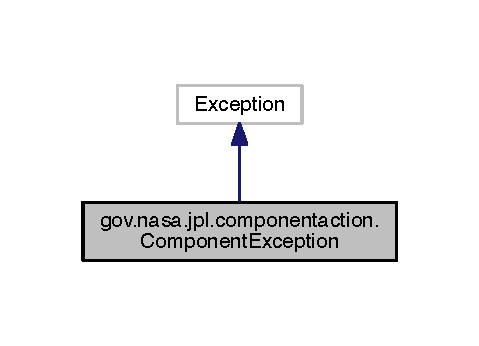
\includegraphics[width=230pt]{classgov_1_1nasa_1_1jpl_1_1componentaction_1_1_component_exception__inherit__graph}
\end{center}
\end{figure}


Collaboration diagram for gov.\+nasa.\+jpl.\+componentaction.\+Component\+Exception\+:
\nopagebreak
\begin{figure}[H]
\begin{center}
\leavevmode
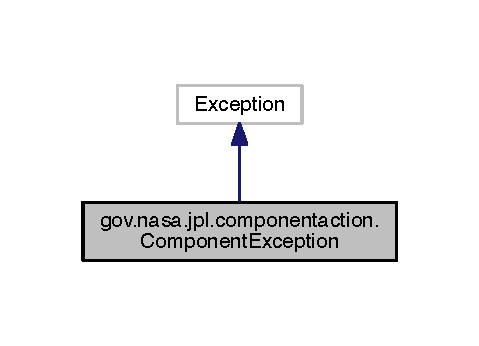
\includegraphics[width=230pt]{classgov_1_1nasa_1_1jpl_1_1componentaction_1_1_component_exception__coll__graph}
\end{center}
\end{figure}
\subsection*{Public Member Functions}
\begin{DoxyCompactItemize}
\item 
{\bf Component\+Exception} (String message)
\end{DoxyCompactItemize}
\subsection*{Static Private Attributes}
\begin{DoxyCompactItemize}
\item 
static final long {\bf serial\+Version\+U\+ID} = 1L
\end{DoxyCompactItemize}


\subsection{Detailed Description}
Component Exception shell class. This just serves as a wrapper that can be used to differentiate between where an error happens. 

\subsection{Constructor \& Destructor Documentation}
\index{gov\+::nasa\+::jpl\+::componentaction\+::\+Component\+Exception@{gov\+::nasa\+::jpl\+::componentaction\+::\+Component\+Exception}!Component\+Exception@{Component\+Exception}}
\index{Component\+Exception@{Component\+Exception}!gov\+::nasa\+::jpl\+::componentaction\+::\+Component\+Exception@{gov\+::nasa\+::jpl\+::componentaction\+::\+Component\+Exception}}
\subsubsection[{Component\+Exception(\+String message)}]{\setlength{\rightskip}{0pt plus 5cm}gov.\+nasa.\+jpl.\+componentaction.\+Component\+Exception.\+Component\+Exception (
\begin{DoxyParamCaption}
\item[{String}]{message}
\end{DoxyParamCaption}
)}\label{classgov_1_1nasa_1_1jpl_1_1componentaction_1_1_component_exception_a30a6dff2a64fde789ee24358383559de}


\subsection{Member Data Documentation}
\index{gov\+::nasa\+::jpl\+::componentaction\+::\+Component\+Exception@{gov\+::nasa\+::jpl\+::componentaction\+::\+Component\+Exception}!serial\+Version\+U\+ID@{serial\+Version\+U\+ID}}
\index{serial\+Version\+U\+ID@{serial\+Version\+U\+ID}!gov\+::nasa\+::jpl\+::componentaction\+::\+Component\+Exception@{gov\+::nasa\+::jpl\+::componentaction\+::\+Component\+Exception}}
\subsubsection[{serial\+Version\+U\+ID}]{\setlength{\rightskip}{0pt plus 5cm}final long gov.\+nasa.\+jpl.\+componentaction.\+Component\+Exception.\+serial\+Version\+U\+ID = 1L\hspace{0.3cm}{\ttfamily [static]}, {\ttfamily [private]}}\label{classgov_1_1nasa_1_1jpl_1_1componentaction_1_1_component_exception_ad5f6a95f567ac0ae10778104cf663b36}


The documentation for this class was generated from the following file\+:\begin{DoxyCompactItemize}
\item 
src/gov/nasa/jpl/componentaction/{\bf Component\+Exception.\+java}\end{DoxyCompactItemize}

\section{gov.\+nasa.\+jpl.\+componentaction.\+I\+S\+F\+Subsystem.\+component\+Type Class Reference}
\label{classgov_1_1nasa_1_1jpl_1_1componentaction_1_1_i_s_f_subsystem_1_1component_type}\index{gov.\+nasa.\+jpl.\+componentaction.\+I\+S\+F\+Subsystem.\+component\+Type@{gov.\+nasa.\+jpl.\+componentaction.\+I\+S\+F\+Subsystem.\+component\+Type}}
\subsection*{Public Member Functions}
\begin{DoxyCompactItemize}
\item 
{\bf component\+Type} ()
\item 
String {\bf get\+Name} ()
\item 
String {\bf get\+Name\+Space} ()
\item 
String {\bf get\+Type} ()
\item 
String {\bf get\+Base\+ID} ()
\item 
String {\bf get\+Instance\+Window} ()
\item 
String {\bf get\+X\+M\+L\+Location} ()
\end{DoxyCompactItemize}
\subsection*{Package Attributes}
\begin{DoxyCompactItemize}
\item 
String {\bf name}
\item 
String {\bf name\+Space}
\item 
String {\bf type}
\item 
String {\bf base\+ID}
\item 
String {\bf instance\+Window}
\item 
String {\bf X\+M\+L\+Location}
\end{DoxyCompactItemize}


\subsection{Detailed Description}
Used as a data\+Objet within the component\+Map. The objects within this object are used to describe a leaf component. The methods are pretty self-\/explanatory. 

\subsection{Constructor \& Destructor Documentation}
\index{gov\+::nasa\+::jpl\+::componentaction\+::\+I\+S\+F\+Subsystem\+::component\+Type@{gov\+::nasa\+::jpl\+::componentaction\+::\+I\+S\+F\+Subsystem\+::component\+Type}!component\+Type@{component\+Type}}
\index{component\+Type@{component\+Type}!gov\+::nasa\+::jpl\+::componentaction\+::\+I\+S\+F\+Subsystem\+::component\+Type@{gov\+::nasa\+::jpl\+::componentaction\+::\+I\+S\+F\+Subsystem\+::component\+Type}}
\subsubsection[{component\+Type()}]{\setlength{\rightskip}{0pt plus 5cm}gov.\+nasa.\+jpl.\+componentaction.\+I\+S\+F\+Subsystem.\+component\+Type.\+component\+Type (
\begin{DoxyParamCaption}
{}
\end{DoxyParamCaption}
)}\label{classgov_1_1nasa_1_1jpl_1_1componentaction_1_1_i_s_f_subsystem_1_1component_type_ad5f6aae82dc798b46b634ebf1a8458b6}


\subsection{Member Function Documentation}
\index{gov\+::nasa\+::jpl\+::componentaction\+::\+I\+S\+F\+Subsystem\+::component\+Type@{gov\+::nasa\+::jpl\+::componentaction\+::\+I\+S\+F\+Subsystem\+::component\+Type}!get\+Base\+ID@{get\+Base\+ID}}
\index{get\+Base\+ID@{get\+Base\+ID}!gov\+::nasa\+::jpl\+::componentaction\+::\+I\+S\+F\+Subsystem\+::component\+Type@{gov\+::nasa\+::jpl\+::componentaction\+::\+I\+S\+F\+Subsystem\+::component\+Type}}
\subsubsection[{get\+Base\+I\+D()}]{\setlength{\rightskip}{0pt plus 5cm}String gov.\+nasa.\+jpl.\+componentaction.\+I\+S\+F\+Subsystem.\+component\+Type.\+get\+Base\+ID (
\begin{DoxyParamCaption}
{}
\end{DoxyParamCaption}
)}\label{classgov_1_1nasa_1_1jpl_1_1componentaction_1_1_i_s_f_subsystem_1_1component_type_affcc0d742e4f0b04a554164adc550d84}
\index{gov\+::nasa\+::jpl\+::componentaction\+::\+I\+S\+F\+Subsystem\+::component\+Type@{gov\+::nasa\+::jpl\+::componentaction\+::\+I\+S\+F\+Subsystem\+::component\+Type}!get\+Instance\+Window@{get\+Instance\+Window}}
\index{get\+Instance\+Window@{get\+Instance\+Window}!gov\+::nasa\+::jpl\+::componentaction\+::\+I\+S\+F\+Subsystem\+::component\+Type@{gov\+::nasa\+::jpl\+::componentaction\+::\+I\+S\+F\+Subsystem\+::component\+Type}}
\subsubsection[{get\+Instance\+Window()}]{\setlength{\rightskip}{0pt plus 5cm}String gov.\+nasa.\+jpl.\+componentaction.\+I\+S\+F\+Subsystem.\+component\+Type.\+get\+Instance\+Window (
\begin{DoxyParamCaption}
{}
\end{DoxyParamCaption}
)}\label{classgov_1_1nasa_1_1jpl_1_1componentaction_1_1_i_s_f_subsystem_1_1component_type_ac592835b8d835a2b5319db44531e6061}
\index{gov\+::nasa\+::jpl\+::componentaction\+::\+I\+S\+F\+Subsystem\+::component\+Type@{gov\+::nasa\+::jpl\+::componentaction\+::\+I\+S\+F\+Subsystem\+::component\+Type}!get\+Name@{get\+Name}}
\index{get\+Name@{get\+Name}!gov\+::nasa\+::jpl\+::componentaction\+::\+I\+S\+F\+Subsystem\+::component\+Type@{gov\+::nasa\+::jpl\+::componentaction\+::\+I\+S\+F\+Subsystem\+::component\+Type}}
\subsubsection[{get\+Name()}]{\setlength{\rightskip}{0pt plus 5cm}String gov.\+nasa.\+jpl.\+componentaction.\+I\+S\+F\+Subsystem.\+component\+Type.\+get\+Name (
\begin{DoxyParamCaption}
{}
\end{DoxyParamCaption}
)}\label{classgov_1_1nasa_1_1jpl_1_1componentaction_1_1_i_s_f_subsystem_1_1component_type_ae6cc5ec807af965816a949163d51cc59}
\index{gov\+::nasa\+::jpl\+::componentaction\+::\+I\+S\+F\+Subsystem\+::component\+Type@{gov\+::nasa\+::jpl\+::componentaction\+::\+I\+S\+F\+Subsystem\+::component\+Type}!get\+Name\+Space@{get\+Name\+Space}}
\index{get\+Name\+Space@{get\+Name\+Space}!gov\+::nasa\+::jpl\+::componentaction\+::\+I\+S\+F\+Subsystem\+::component\+Type@{gov\+::nasa\+::jpl\+::componentaction\+::\+I\+S\+F\+Subsystem\+::component\+Type}}
\subsubsection[{get\+Name\+Space()}]{\setlength{\rightskip}{0pt plus 5cm}String gov.\+nasa.\+jpl.\+componentaction.\+I\+S\+F\+Subsystem.\+component\+Type.\+get\+Name\+Space (
\begin{DoxyParamCaption}
{}
\end{DoxyParamCaption}
)}\label{classgov_1_1nasa_1_1jpl_1_1componentaction_1_1_i_s_f_subsystem_1_1component_type_aa6685a55445c7dd66f0f0a97d33b493f}
\index{gov\+::nasa\+::jpl\+::componentaction\+::\+I\+S\+F\+Subsystem\+::component\+Type@{gov\+::nasa\+::jpl\+::componentaction\+::\+I\+S\+F\+Subsystem\+::component\+Type}!get\+Type@{get\+Type}}
\index{get\+Type@{get\+Type}!gov\+::nasa\+::jpl\+::componentaction\+::\+I\+S\+F\+Subsystem\+::component\+Type@{gov\+::nasa\+::jpl\+::componentaction\+::\+I\+S\+F\+Subsystem\+::component\+Type}}
\subsubsection[{get\+Type()}]{\setlength{\rightskip}{0pt plus 5cm}String gov.\+nasa.\+jpl.\+componentaction.\+I\+S\+F\+Subsystem.\+component\+Type.\+get\+Type (
\begin{DoxyParamCaption}
{}
\end{DoxyParamCaption}
)}\label{classgov_1_1nasa_1_1jpl_1_1componentaction_1_1_i_s_f_subsystem_1_1component_type_a56cb87c9fadaa416e52ade20993a5eca}
\index{gov\+::nasa\+::jpl\+::componentaction\+::\+I\+S\+F\+Subsystem\+::component\+Type@{gov\+::nasa\+::jpl\+::componentaction\+::\+I\+S\+F\+Subsystem\+::component\+Type}!get\+X\+M\+L\+Location@{get\+X\+M\+L\+Location}}
\index{get\+X\+M\+L\+Location@{get\+X\+M\+L\+Location}!gov\+::nasa\+::jpl\+::componentaction\+::\+I\+S\+F\+Subsystem\+::component\+Type@{gov\+::nasa\+::jpl\+::componentaction\+::\+I\+S\+F\+Subsystem\+::component\+Type}}
\subsubsection[{get\+X\+M\+L\+Location()}]{\setlength{\rightskip}{0pt plus 5cm}String gov.\+nasa.\+jpl.\+componentaction.\+I\+S\+F\+Subsystem.\+component\+Type.\+get\+X\+M\+L\+Location (
\begin{DoxyParamCaption}
{}
\end{DoxyParamCaption}
)}\label{classgov_1_1nasa_1_1jpl_1_1componentaction_1_1_i_s_f_subsystem_1_1component_type_a4406620698b686ca4b2da8d2a5a14559}


\subsection{Member Data Documentation}
\index{gov\+::nasa\+::jpl\+::componentaction\+::\+I\+S\+F\+Subsystem\+::component\+Type@{gov\+::nasa\+::jpl\+::componentaction\+::\+I\+S\+F\+Subsystem\+::component\+Type}!base\+ID@{base\+ID}}
\index{base\+ID@{base\+ID}!gov\+::nasa\+::jpl\+::componentaction\+::\+I\+S\+F\+Subsystem\+::component\+Type@{gov\+::nasa\+::jpl\+::componentaction\+::\+I\+S\+F\+Subsystem\+::component\+Type}}
\subsubsection[{base\+ID}]{\setlength{\rightskip}{0pt plus 5cm}String gov.\+nasa.\+jpl.\+componentaction.\+I\+S\+F\+Subsystem.\+component\+Type.\+base\+ID\hspace{0.3cm}{\ttfamily [package]}}\label{classgov_1_1nasa_1_1jpl_1_1componentaction_1_1_i_s_f_subsystem_1_1component_type_ad5d0f8c21b37411a06b0f3f86b3e5ab1}
\index{gov\+::nasa\+::jpl\+::componentaction\+::\+I\+S\+F\+Subsystem\+::component\+Type@{gov\+::nasa\+::jpl\+::componentaction\+::\+I\+S\+F\+Subsystem\+::component\+Type}!instance\+Window@{instance\+Window}}
\index{instance\+Window@{instance\+Window}!gov\+::nasa\+::jpl\+::componentaction\+::\+I\+S\+F\+Subsystem\+::component\+Type@{gov\+::nasa\+::jpl\+::componentaction\+::\+I\+S\+F\+Subsystem\+::component\+Type}}
\subsubsection[{instance\+Window}]{\setlength{\rightskip}{0pt plus 5cm}String gov.\+nasa.\+jpl.\+componentaction.\+I\+S\+F\+Subsystem.\+component\+Type.\+instance\+Window\hspace{0.3cm}{\ttfamily [package]}}\label{classgov_1_1nasa_1_1jpl_1_1componentaction_1_1_i_s_f_subsystem_1_1component_type_a2586b6c96e5a1167c4dc1229d9c8a13d}
\index{gov\+::nasa\+::jpl\+::componentaction\+::\+I\+S\+F\+Subsystem\+::component\+Type@{gov\+::nasa\+::jpl\+::componentaction\+::\+I\+S\+F\+Subsystem\+::component\+Type}!name@{name}}
\index{name@{name}!gov\+::nasa\+::jpl\+::componentaction\+::\+I\+S\+F\+Subsystem\+::component\+Type@{gov\+::nasa\+::jpl\+::componentaction\+::\+I\+S\+F\+Subsystem\+::component\+Type}}
\subsubsection[{name}]{\setlength{\rightskip}{0pt plus 5cm}String gov.\+nasa.\+jpl.\+componentaction.\+I\+S\+F\+Subsystem.\+component\+Type.\+name\hspace{0.3cm}{\ttfamily [package]}}\label{classgov_1_1nasa_1_1jpl_1_1componentaction_1_1_i_s_f_subsystem_1_1component_type_aebb6bf0047764ae646b84f167be9c388}
\index{gov\+::nasa\+::jpl\+::componentaction\+::\+I\+S\+F\+Subsystem\+::component\+Type@{gov\+::nasa\+::jpl\+::componentaction\+::\+I\+S\+F\+Subsystem\+::component\+Type}!name\+Space@{name\+Space}}
\index{name\+Space@{name\+Space}!gov\+::nasa\+::jpl\+::componentaction\+::\+I\+S\+F\+Subsystem\+::component\+Type@{gov\+::nasa\+::jpl\+::componentaction\+::\+I\+S\+F\+Subsystem\+::component\+Type}}
\subsubsection[{name\+Space}]{\setlength{\rightskip}{0pt plus 5cm}String gov.\+nasa.\+jpl.\+componentaction.\+I\+S\+F\+Subsystem.\+component\+Type.\+name\+Space\hspace{0.3cm}{\ttfamily [package]}}\label{classgov_1_1nasa_1_1jpl_1_1componentaction_1_1_i_s_f_subsystem_1_1component_type_af5198d50a82ad857c1143492838d456b}
\index{gov\+::nasa\+::jpl\+::componentaction\+::\+I\+S\+F\+Subsystem\+::component\+Type@{gov\+::nasa\+::jpl\+::componentaction\+::\+I\+S\+F\+Subsystem\+::component\+Type}!type@{type}}
\index{type@{type}!gov\+::nasa\+::jpl\+::componentaction\+::\+I\+S\+F\+Subsystem\+::component\+Type@{gov\+::nasa\+::jpl\+::componentaction\+::\+I\+S\+F\+Subsystem\+::component\+Type}}
\subsubsection[{type}]{\setlength{\rightskip}{0pt plus 5cm}String gov.\+nasa.\+jpl.\+componentaction.\+I\+S\+F\+Subsystem.\+component\+Type.\+type\hspace{0.3cm}{\ttfamily [package]}}\label{classgov_1_1nasa_1_1jpl_1_1componentaction_1_1_i_s_f_subsystem_1_1component_type_a2e805920fb78f5913085d9b16dfa1220}
\index{gov\+::nasa\+::jpl\+::componentaction\+::\+I\+S\+F\+Subsystem\+::component\+Type@{gov\+::nasa\+::jpl\+::componentaction\+::\+I\+S\+F\+Subsystem\+::component\+Type}!X\+M\+L\+Location@{X\+M\+L\+Location}}
\index{X\+M\+L\+Location@{X\+M\+L\+Location}!gov\+::nasa\+::jpl\+::componentaction\+::\+I\+S\+F\+Subsystem\+::component\+Type@{gov\+::nasa\+::jpl\+::componentaction\+::\+I\+S\+F\+Subsystem\+::component\+Type}}
\subsubsection[{X\+M\+L\+Location}]{\setlength{\rightskip}{0pt plus 5cm}String gov.\+nasa.\+jpl.\+componentaction.\+I\+S\+F\+Subsystem.\+component\+Type.\+X\+M\+L\+Location\hspace{0.3cm}{\ttfamily [package]}}\label{classgov_1_1nasa_1_1jpl_1_1componentaction_1_1_i_s_f_subsystem_1_1component_type_ac545f9b7365e3bb8c9d823be84395f37}


The documentation for this class was generated from the following file\+:\begin{DoxyCompactItemize}
\item 
src/gov/nasa/jpl/componentaction/{\bf I\+S\+F\+Subsystem.\+java}\end{DoxyCompactItemize}

\section{gov.\+nasa.\+jpl.\+componentaction.\+Load\+I\+D\+Config.\+config\+Item Class Reference}
\label{classgov_1_1nasa_1_1jpl_1_1componentaction_1_1_load_i_d_config_1_1config_item}\index{gov.\+nasa.\+jpl.\+componentaction.\+Load\+I\+D\+Config.\+config\+Item@{gov.\+nasa.\+jpl.\+componentaction.\+Load\+I\+D\+Config.\+config\+Item}}
\subsection*{Public Member Functions}
\begin{DoxyCompactItemize}
\item 
{\bf config\+Item} (String comp\+Type, String inst\+Name, int b\+ID, int w\+Range)
\item 
int {\bf hash\+Code} ()
\item 
boolean {\bf equals} (Object obj)
\item 
String {\bf to\+String} ()
\end{DoxyCompactItemize}
\subsection*{Package Attributes}
\begin{DoxyCompactItemize}
\item 
String {\bf component\+Type}
\item 
String {\bf instance\+Name}
\item 
int {\bf base\+ID}
\item 
int {\bf window\+Range}
\end{DoxyCompactItemize}


\subsection{Detailed Description}
Used to store information for each configuration item from the config file. 

\subsection{Constructor \& Destructor Documentation}
\index{gov\+::nasa\+::jpl\+::componentaction\+::\+Load\+I\+D\+Config\+::config\+Item@{gov\+::nasa\+::jpl\+::componentaction\+::\+Load\+I\+D\+Config\+::config\+Item}!config\+Item@{config\+Item}}
\index{config\+Item@{config\+Item}!gov\+::nasa\+::jpl\+::componentaction\+::\+Load\+I\+D\+Config\+::config\+Item@{gov\+::nasa\+::jpl\+::componentaction\+::\+Load\+I\+D\+Config\+::config\+Item}}
\subsubsection[{config\+Item(\+String comp\+Type, String inst\+Name, int b\+I\+D, int w\+Range)}]{\setlength{\rightskip}{0pt plus 5cm}gov.\+nasa.\+jpl.\+componentaction.\+Load\+I\+D\+Config.\+config\+Item.\+config\+Item (
\begin{DoxyParamCaption}
\item[{String}]{comp\+Type, }
\item[{String}]{inst\+Name, }
\item[{int}]{b\+ID, }
\item[{int}]{w\+Range}
\end{DoxyParamCaption}
)}\label{classgov_1_1nasa_1_1jpl_1_1componentaction_1_1_load_i_d_config_1_1config_item_a56b0f04d87985eadd41f0df6c49fb2cf}


Here is the caller graph for this function\+:
\nopagebreak
\begin{figure}[H]
\begin{center}
\leavevmode
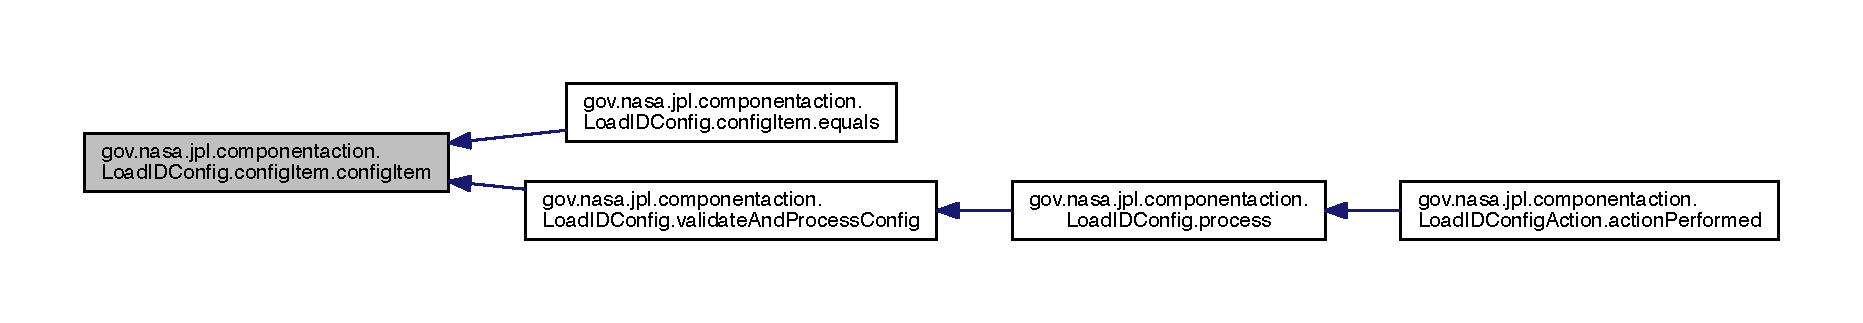
\includegraphics[width=350pt]{classgov_1_1nasa_1_1jpl_1_1componentaction_1_1_load_i_d_config_1_1config_item_a56b0f04d87985eadd41f0df6c49fb2cf_icgraph}
\end{center}
\end{figure}




\subsection{Member Function Documentation}
\index{gov\+::nasa\+::jpl\+::componentaction\+::\+Load\+I\+D\+Config\+::config\+Item@{gov\+::nasa\+::jpl\+::componentaction\+::\+Load\+I\+D\+Config\+::config\+Item}!equals@{equals}}
\index{equals@{equals}!gov\+::nasa\+::jpl\+::componentaction\+::\+Load\+I\+D\+Config\+::config\+Item@{gov\+::nasa\+::jpl\+::componentaction\+::\+Load\+I\+D\+Config\+::config\+Item}}
\subsubsection[{equals(\+Object obj)}]{\setlength{\rightskip}{0pt plus 5cm}boolean gov.\+nasa.\+jpl.\+componentaction.\+Load\+I\+D\+Config.\+config\+Item.\+equals (
\begin{DoxyParamCaption}
\item[{Object}]{obj}
\end{DoxyParamCaption}
)}\label{classgov_1_1nasa_1_1jpl_1_1componentaction_1_1_load_i_d_config_1_1config_item_a6d41eae19afb1b06c786111c4a5fad20}


Here is the call graph for this function\+:
\nopagebreak
\begin{figure}[H]
\begin{center}
\leavevmode
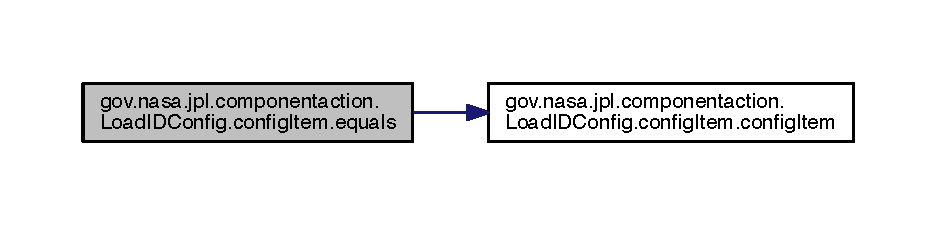
\includegraphics[width=350pt]{classgov_1_1nasa_1_1jpl_1_1componentaction_1_1_load_i_d_config_1_1config_item_a6d41eae19afb1b06c786111c4a5fad20_cgraph}
\end{center}
\end{figure}


\index{gov\+::nasa\+::jpl\+::componentaction\+::\+Load\+I\+D\+Config\+::config\+Item@{gov\+::nasa\+::jpl\+::componentaction\+::\+Load\+I\+D\+Config\+::config\+Item}!hash\+Code@{hash\+Code}}
\index{hash\+Code@{hash\+Code}!gov\+::nasa\+::jpl\+::componentaction\+::\+Load\+I\+D\+Config\+::config\+Item@{gov\+::nasa\+::jpl\+::componentaction\+::\+Load\+I\+D\+Config\+::config\+Item}}
\subsubsection[{hash\+Code()}]{\setlength{\rightskip}{0pt plus 5cm}int gov.\+nasa.\+jpl.\+componentaction.\+Load\+I\+D\+Config.\+config\+Item.\+hash\+Code (
\begin{DoxyParamCaption}
{}
\end{DoxyParamCaption}
)}\label{classgov_1_1nasa_1_1jpl_1_1componentaction_1_1_load_i_d_config_1_1config_item_a87dd7a9c670b8d325c7bd944e41c0c6c}
\index{gov\+::nasa\+::jpl\+::componentaction\+::\+Load\+I\+D\+Config\+::config\+Item@{gov\+::nasa\+::jpl\+::componentaction\+::\+Load\+I\+D\+Config\+::config\+Item}!to\+String@{to\+String}}
\index{to\+String@{to\+String}!gov\+::nasa\+::jpl\+::componentaction\+::\+Load\+I\+D\+Config\+::config\+Item@{gov\+::nasa\+::jpl\+::componentaction\+::\+Load\+I\+D\+Config\+::config\+Item}}
\subsubsection[{to\+String()}]{\setlength{\rightskip}{0pt plus 5cm}String gov.\+nasa.\+jpl.\+componentaction.\+Load\+I\+D\+Config.\+config\+Item.\+to\+String (
\begin{DoxyParamCaption}
{}
\end{DoxyParamCaption}
)}\label{classgov_1_1nasa_1_1jpl_1_1componentaction_1_1_load_i_d_config_1_1config_item_a5b143dcfac8d1bb37777d79a5be0082f}


\subsection{Member Data Documentation}
\index{gov\+::nasa\+::jpl\+::componentaction\+::\+Load\+I\+D\+Config\+::config\+Item@{gov\+::nasa\+::jpl\+::componentaction\+::\+Load\+I\+D\+Config\+::config\+Item}!base\+ID@{base\+ID}}
\index{base\+ID@{base\+ID}!gov\+::nasa\+::jpl\+::componentaction\+::\+Load\+I\+D\+Config\+::config\+Item@{gov\+::nasa\+::jpl\+::componentaction\+::\+Load\+I\+D\+Config\+::config\+Item}}
\subsubsection[{base\+ID}]{\setlength{\rightskip}{0pt plus 5cm}int gov.\+nasa.\+jpl.\+componentaction.\+Load\+I\+D\+Config.\+config\+Item.\+base\+ID\hspace{0.3cm}{\ttfamily [package]}}\label{classgov_1_1nasa_1_1jpl_1_1componentaction_1_1_load_i_d_config_1_1config_item_a31fc0d6dd8c32acbfb098b295054b4e3}
\index{gov\+::nasa\+::jpl\+::componentaction\+::\+Load\+I\+D\+Config\+::config\+Item@{gov\+::nasa\+::jpl\+::componentaction\+::\+Load\+I\+D\+Config\+::config\+Item}!component\+Type@{component\+Type}}
\index{component\+Type@{component\+Type}!gov\+::nasa\+::jpl\+::componentaction\+::\+Load\+I\+D\+Config\+::config\+Item@{gov\+::nasa\+::jpl\+::componentaction\+::\+Load\+I\+D\+Config\+::config\+Item}}
\subsubsection[{component\+Type}]{\setlength{\rightskip}{0pt plus 5cm}String gov.\+nasa.\+jpl.\+componentaction.\+Load\+I\+D\+Config.\+config\+Item.\+component\+Type\hspace{0.3cm}{\ttfamily [package]}}\label{classgov_1_1nasa_1_1jpl_1_1componentaction_1_1_load_i_d_config_1_1config_item_a5acb18e8dfde633e1a207ff47df30b78}
\index{gov\+::nasa\+::jpl\+::componentaction\+::\+Load\+I\+D\+Config\+::config\+Item@{gov\+::nasa\+::jpl\+::componentaction\+::\+Load\+I\+D\+Config\+::config\+Item}!instance\+Name@{instance\+Name}}
\index{instance\+Name@{instance\+Name}!gov\+::nasa\+::jpl\+::componentaction\+::\+Load\+I\+D\+Config\+::config\+Item@{gov\+::nasa\+::jpl\+::componentaction\+::\+Load\+I\+D\+Config\+::config\+Item}}
\subsubsection[{instance\+Name}]{\setlength{\rightskip}{0pt plus 5cm}String gov.\+nasa.\+jpl.\+componentaction.\+Load\+I\+D\+Config.\+config\+Item.\+instance\+Name\hspace{0.3cm}{\ttfamily [package]}}\label{classgov_1_1nasa_1_1jpl_1_1componentaction_1_1_load_i_d_config_1_1config_item_a60a83550bd2740ae1c6fb4e78a6503e4}
\index{gov\+::nasa\+::jpl\+::componentaction\+::\+Load\+I\+D\+Config\+::config\+Item@{gov\+::nasa\+::jpl\+::componentaction\+::\+Load\+I\+D\+Config\+::config\+Item}!window\+Range@{window\+Range}}
\index{window\+Range@{window\+Range}!gov\+::nasa\+::jpl\+::componentaction\+::\+Load\+I\+D\+Config\+::config\+Item@{gov\+::nasa\+::jpl\+::componentaction\+::\+Load\+I\+D\+Config\+::config\+Item}}
\subsubsection[{window\+Range}]{\setlength{\rightskip}{0pt plus 5cm}int gov.\+nasa.\+jpl.\+componentaction.\+Load\+I\+D\+Config.\+config\+Item.\+window\+Range\hspace{0.3cm}{\ttfamily [package]}}\label{classgov_1_1nasa_1_1jpl_1_1componentaction_1_1_load_i_d_config_1_1config_item_ae8642cf0f020519eb9357dca404e61ce}


The documentation for this class was generated from the following file\+:\begin{DoxyCompactItemize}
\item 
src/gov/nasa/jpl/componentaction/{\bf Load\+I\+D\+Config.\+java}\end{DoxyCompactItemize}

\section{gov.\+nasa.\+jpl.\+componentaction.\+Connector\+Exception Class Reference}
\label{classgov_1_1nasa_1_1jpl_1_1componentaction_1_1_connector_exception}\index{gov.\+nasa.\+jpl.\+componentaction.\+Connector\+Exception@{gov.\+nasa.\+jpl.\+componentaction.\+Connector\+Exception}}


Inheritance diagram for gov.\+nasa.\+jpl.\+componentaction.\+Connector\+Exception\+:
\nopagebreak
\begin{figure}[H]
\begin{center}
\leavevmode
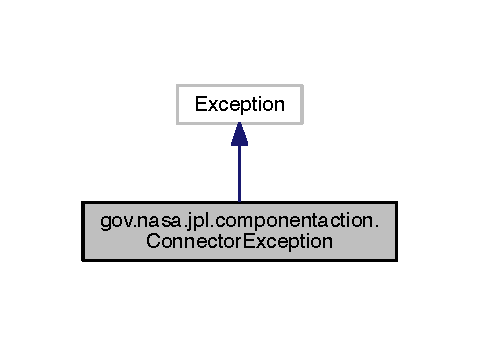
\includegraphics[width=230pt]{classgov_1_1nasa_1_1jpl_1_1componentaction_1_1_connector_exception__inherit__graph}
\end{center}
\end{figure}


Collaboration diagram for gov.\+nasa.\+jpl.\+componentaction.\+Connector\+Exception\+:
\nopagebreak
\begin{figure}[H]
\begin{center}
\leavevmode
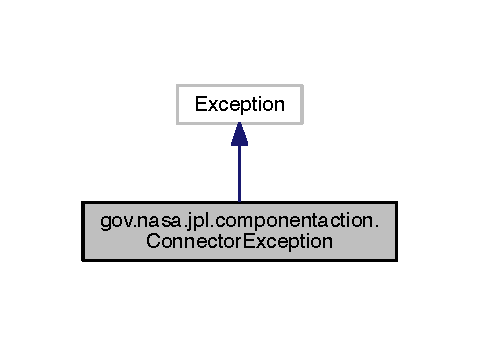
\includegraphics[width=230pt]{classgov_1_1nasa_1_1jpl_1_1componentaction_1_1_connector_exception__coll__graph}
\end{center}
\end{figure}
\subsection*{Public Member Functions}
\begin{DoxyCompactItemize}
\item 
{\bf Connector\+Exception} (String message)
\end{DoxyCompactItemize}
\subsection*{Static Private Attributes}
\begin{DoxyCompactItemize}
\item 
static final long {\bf serial\+Version\+U\+ID} = 1L
\end{DoxyCompactItemize}


\subsection{Detailed Description}
Connector Exception shell class. This just serves as a wrapper that can be used to differentiate between where an error happens. 

\subsection{Constructor \& Destructor Documentation}
\index{gov\+::nasa\+::jpl\+::componentaction\+::\+Connector\+Exception@{gov\+::nasa\+::jpl\+::componentaction\+::\+Connector\+Exception}!Connector\+Exception@{Connector\+Exception}}
\index{Connector\+Exception@{Connector\+Exception}!gov\+::nasa\+::jpl\+::componentaction\+::\+Connector\+Exception@{gov\+::nasa\+::jpl\+::componentaction\+::\+Connector\+Exception}}
\subsubsection[{Connector\+Exception(\+String message)}]{\setlength{\rightskip}{0pt plus 5cm}gov.\+nasa.\+jpl.\+componentaction.\+Connector\+Exception.\+Connector\+Exception (
\begin{DoxyParamCaption}
\item[{String}]{message}
\end{DoxyParamCaption}
)}\label{classgov_1_1nasa_1_1jpl_1_1componentaction_1_1_connector_exception_ac8b39058457b48f0729fd38d38555442}


\subsection{Member Data Documentation}
\index{gov\+::nasa\+::jpl\+::componentaction\+::\+Connector\+Exception@{gov\+::nasa\+::jpl\+::componentaction\+::\+Connector\+Exception}!serial\+Version\+U\+ID@{serial\+Version\+U\+ID}}
\index{serial\+Version\+U\+ID@{serial\+Version\+U\+ID}!gov\+::nasa\+::jpl\+::componentaction\+::\+Connector\+Exception@{gov\+::nasa\+::jpl\+::componentaction\+::\+Connector\+Exception}}
\subsubsection[{serial\+Version\+U\+ID}]{\setlength{\rightskip}{0pt plus 5cm}final long gov.\+nasa.\+jpl.\+componentaction.\+Connector\+Exception.\+serial\+Version\+U\+ID = 1L\hspace{0.3cm}{\ttfamily [static]}, {\ttfamily [private]}}\label{classgov_1_1nasa_1_1jpl_1_1componentaction_1_1_connector_exception_a95f0f185bf2d2f3806705333dc3a9787}


The documentation for this class was generated from the following file\+:\begin{DoxyCompactItemize}
\item 
src/gov/nasa/jpl/componentaction/{\bf Connector\+Exception.\+java}\end{DoxyCompactItemize}

\section{gov.\+nasa.\+jpl.\+componentaction.\+Isf\+About Class Reference}
\label{classgov_1_1nasa_1_1jpl_1_1componentaction_1_1_isf_about}\index{gov.\+nasa.\+jpl.\+componentaction.\+Isf\+About@{gov.\+nasa.\+jpl.\+componentaction.\+Isf\+About}}


Inheritance diagram for gov.\+nasa.\+jpl.\+componentaction.\+Isf\+About\+:
\nopagebreak
\begin{figure}[H]
\begin{center}
\leavevmode
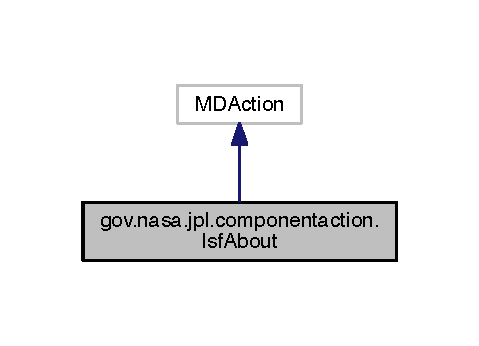
\includegraphics[width=230pt]{classgov_1_1nasa_1_1jpl_1_1componentaction_1_1_isf_about__inherit__graph}
\end{center}
\end{figure}


Collaboration diagram for gov.\+nasa.\+jpl.\+componentaction.\+Isf\+About\+:
\nopagebreak
\begin{figure}[H]
\begin{center}
\leavevmode
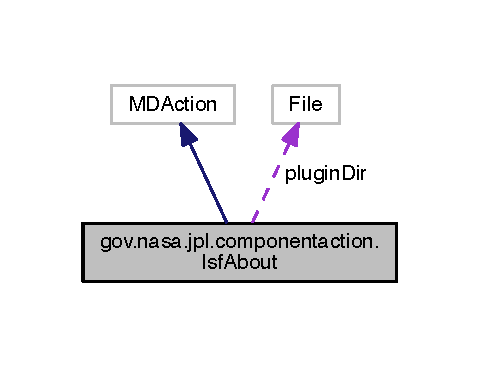
\includegraphics[width=230pt]{classgov_1_1nasa_1_1jpl_1_1componentaction_1_1_isf_about__coll__graph}
\end{center}
\end{figure}
\subsection*{Public Member Functions}
\begin{DoxyCompactItemize}
\item 
{\bf Isf\+About} (String id, String name, File {\bf plugin\+Dir})
\item 
void {\bf action\+Performed} (Action\+Event e)
\end{DoxyCompactItemize}
\subsection*{Package Attributes}
\begin{DoxyCompactItemize}
\item 
File {\bf plugin\+Dir}
\end{DoxyCompactItemize}
\subsection*{Static Private Attributes}
\begin{DoxyCompactItemize}
\item 
static final long {\bf serial\+Version\+U\+ID} = -\/6790954285526957354L
\end{DoxyCompactItemize}


\subsection{Detailed Description}
Action class for information regarding the plugin 

\subsection{Constructor \& Destructor Documentation}
\index{gov\+::nasa\+::jpl\+::componentaction\+::\+Isf\+About@{gov\+::nasa\+::jpl\+::componentaction\+::\+Isf\+About}!Isf\+About@{Isf\+About}}
\index{Isf\+About@{Isf\+About}!gov\+::nasa\+::jpl\+::componentaction\+::\+Isf\+About@{gov\+::nasa\+::jpl\+::componentaction\+::\+Isf\+About}}
\subsubsection[{Isf\+About(\+String id, String name, File plugin\+Dir)}]{\setlength{\rightskip}{0pt plus 5cm}gov.\+nasa.\+jpl.\+componentaction.\+Isf\+About.\+Isf\+About (
\begin{DoxyParamCaption}
\item[{String}]{id, }
\item[{String}]{name, }
\item[{File}]{plugin\+Dir}
\end{DoxyParamCaption}
)}\label{classgov_1_1nasa_1_1jpl_1_1componentaction_1_1_isf_about_ac57c8dda5bfd3feb1bab24f8e01fdf37}


\subsection{Member Function Documentation}
\index{gov\+::nasa\+::jpl\+::componentaction\+::\+Isf\+About@{gov\+::nasa\+::jpl\+::componentaction\+::\+Isf\+About}!action\+Performed@{action\+Performed}}
\index{action\+Performed@{action\+Performed}!gov\+::nasa\+::jpl\+::componentaction\+::\+Isf\+About@{gov\+::nasa\+::jpl\+::componentaction\+::\+Isf\+About}}
\subsubsection[{action\+Performed(\+Action\+Event e)}]{\setlength{\rightskip}{0pt plus 5cm}void gov.\+nasa.\+jpl.\+componentaction.\+Isf\+About.\+action\+Performed (
\begin{DoxyParamCaption}
\item[{Action\+Event}]{e}
\end{DoxyParamCaption}
)}\label{classgov_1_1nasa_1_1jpl_1_1componentaction_1_1_isf_about_ae970fc57832b28e4edcb23ed3387c625}
Used to display content in the \char`\"{}\+About\char`\"{} tab. Edit this for tab changes. 

Here is the caller graph for this function\+:
\nopagebreak
\begin{figure}[H]
\begin{center}
\leavevmode
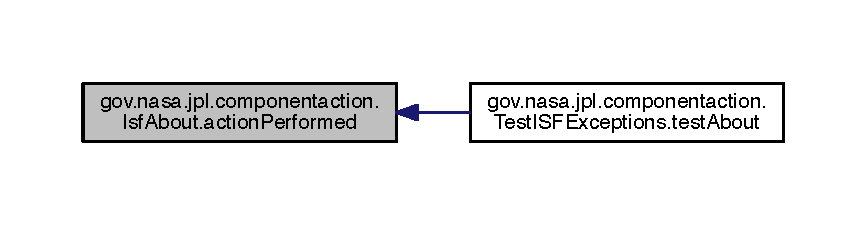
\includegraphics[width=350pt]{classgov_1_1nasa_1_1jpl_1_1componentaction_1_1_isf_about_ae970fc57832b28e4edcb23ed3387c625_icgraph}
\end{center}
\end{figure}




\subsection{Member Data Documentation}
\index{gov\+::nasa\+::jpl\+::componentaction\+::\+Isf\+About@{gov\+::nasa\+::jpl\+::componentaction\+::\+Isf\+About}!plugin\+Dir@{plugin\+Dir}}
\index{plugin\+Dir@{plugin\+Dir}!gov\+::nasa\+::jpl\+::componentaction\+::\+Isf\+About@{gov\+::nasa\+::jpl\+::componentaction\+::\+Isf\+About}}
\subsubsection[{plugin\+Dir}]{\setlength{\rightskip}{0pt plus 5cm}File gov.\+nasa.\+jpl.\+componentaction.\+Isf\+About.\+plugin\+Dir\hspace{0.3cm}{\ttfamily [package]}}\label{classgov_1_1nasa_1_1jpl_1_1componentaction_1_1_isf_about_a251811c6f1965e8906ab409fe871019a}
\index{gov\+::nasa\+::jpl\+::componentaction\+::\+Isf\+About@{gov\+::nasa\+::jpl\+::componentaction\+::\+Isf\+About}!serial\+Version\+U\+ID@{serial\+Version\+U\+ID}}
\index{serial\+Version\+U\+ID@{serial\+Version\+U\+ID}!gov\+::nasa\+::jpl\+::componentaction\+::\+Isf\+About@{gov\+::nasa\+::jpl\+::componentaction\+::\+Isf\+About}}
\subsubsection[{serial\+Version\+U\+ID}]{\setlength{\rightskip}{0pt plus 5cm}final long gov.\+nasa.\+jpl.\+componentaction.\+Isf\+About.\+serial\+Version\+U\+ID = -\/6790954285526957354L\hspace{0.3cm}{\ttfamily [static]}, {\ttfamily [private]}}\label{classgov_1_1nasa_1_1jpl_1_1componentaction_1_1_isf_about_ae12e0ab260ed45d1924c6f549e8e0d8c}


The documentation for this class was generated from the following file\+:\begin{DoxyCompactItemize}
\item 
src/gov/nasa/jpl/componentaction/{\bf Isf\+About.\+java}\end{DoxyCompactItemize}

\section{gov.\+nasa.\+jpl.\+componentaction.\+Isf\+Command\+Line Class Reference}
\label{classgov_1_1nasa_1_1jpl_1_1componentaction_1_1_isf_command_line}\index{gov.\+nasa.\+jpl.\+componentaction.\+Isf\+Command\+Line@{gov.\+nasa.\+jpl.\+componentaction.\+Isf\+Command\+Line}}


Inheritance diagram for gov.\+nasa.\+jpl.\+componentaction.\+Isf\+Command\+Line\+:
\nopagebreak
\begin{figure}[H]
\begin{center}
\leavevmode
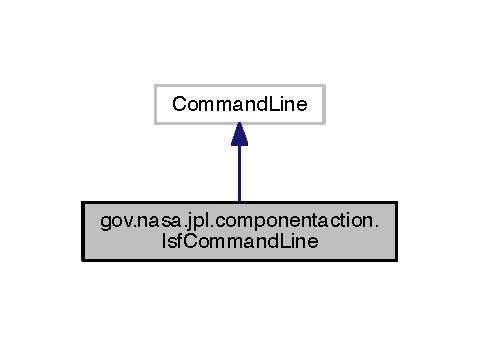
\includegraphics[width=230pt]{classgov_1_1nasa_1_1jpl_1_1componentaction_1_1_isf_command_line__inherit__graph}
\end{center}
\end{figure}


Collaboration diagram for gov.\+nasa.\+jpl.\+componentaction.\+Isf\+Command\+Line\+:
\nopagebreak
\begin{figure}[H]
\begin{center}
\leavevmode
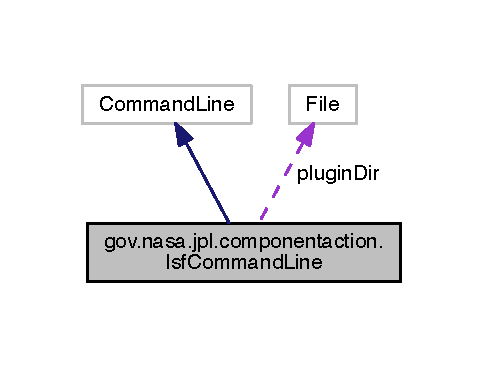
\includegraphics[width=232pt]{classgov_1_1nasa_1_1jpl_1_1componentaction_1_1_isf_command_line__coll__graph}
\end{center}
\end{figure}
\subsection*{Static Public Member Functions}
\begin{DoxyCompactItemize}
\item 
static void {\bf main} (String[$\,$] args)
\end{DoxyCompactItemize}
\subsection*{Protected Member Functions}
\begin{DoxyCompactItemize}
\item 
byte {\bf execute} ()
\end{DoxyCompactItemize}
\subsection*{Static Package Attributes}
\begin{DoxyCompactItemize}
\item 
static File {\bf plugin\+Dir}
\item 
static String {\bf project\+File}
\end{DoxyCompactItemize}
\subsection*{Static Private Attributes}
\begin{DoxyCompactItemize}
\item 
static final String {\bf P\+R\+O\+J\+E\+CT} = \char`\"{}project\+\_\+name\char`\"{}
\item 
static final String {\bf P\+A\+C\+K\+A\+GE} = \char`\"{}package\char`\"{}
\item 
static final String {\bf U\+S\+A\+GE} = \char`\"{}isfpluginexec [options]\textbackslash{}n\+Before running on headless environment, use Xvfb to set up a virtual X11 display server\textbackslash{}n/usr/bin/Xvfb \+:1 -\/screen 0 1024x768x24\textbackslash{}nexport D\+I\+S\+P\+L\+A\+Y=\+:1\char`\"{}
\item 
static final String {\bf C\+O\+P\+Y\+R\+I\+G\+HT} = \char`\"{}Copyright 2015 (California Institute of Technology)\textbackslash{}n\+A\+LL R\+I\+G\+H\+TS R\+E\+S\+E\+R\+V\+E\+D. U.\+S. Government Sponsorship acknowledged.\char`\"{}
\end{DoxyCompactItemize}


\subsection{Detailed Description}
Class to run Magic\+Draw plugin from command line

Before running on headless environment, use Xvfb to set up a virtual X11 display server {\ttfamily /usr/bin/\+Xvfb \+:1 -\/screen 0 1024x768x24 export D\+I\+S\+P\+L\+AY=\+:1 }

To run the utility, use the script isfpluginexec.\+sh in the Magic\+Draw\+Comd\+Plugin directory 

\subsection{Member Function Documentation}
\index{gov\+::nasa\+::jpl\+::componentaction\+::\+Isf\+Command\+Line@{gov\+::nasa\+::jpl\+::componentaction\+::\+Isf\+Command\+Line}!execute@{execute}}
\index{execute@{execute}!gov\+::nasa\+::jpl\+::componentaction\+::\+Isf\+Command\+Line@{gov\+::nasa\+::jpl\+::componentaction\+::\+Isf\+Command\+Line}}
\subsubsection[{execute()}]{\setlength{\rightskip}{0pt plus 5cm}byte gov.\+nasa.\+jpl.\+componentaction.\+Isf\+Command\+Line.\+execute (
\begin{DoxyParamCaption}
{}
\end{DoxyParamCaption}
)\hspace{0.3cm}{\ttfamily [protected]}}\label{classgov_1_1nasa_1_1jpl_1_1componentaction_1_1_isf_command_line_ae4b2178b8721a8ec817fc16c75613b99}
Runs autocoder on the project specified 

Here is the call graph for this function\+:
\nopagebreak
\begin{figure}[H]
\begin{center}
\leavevmode
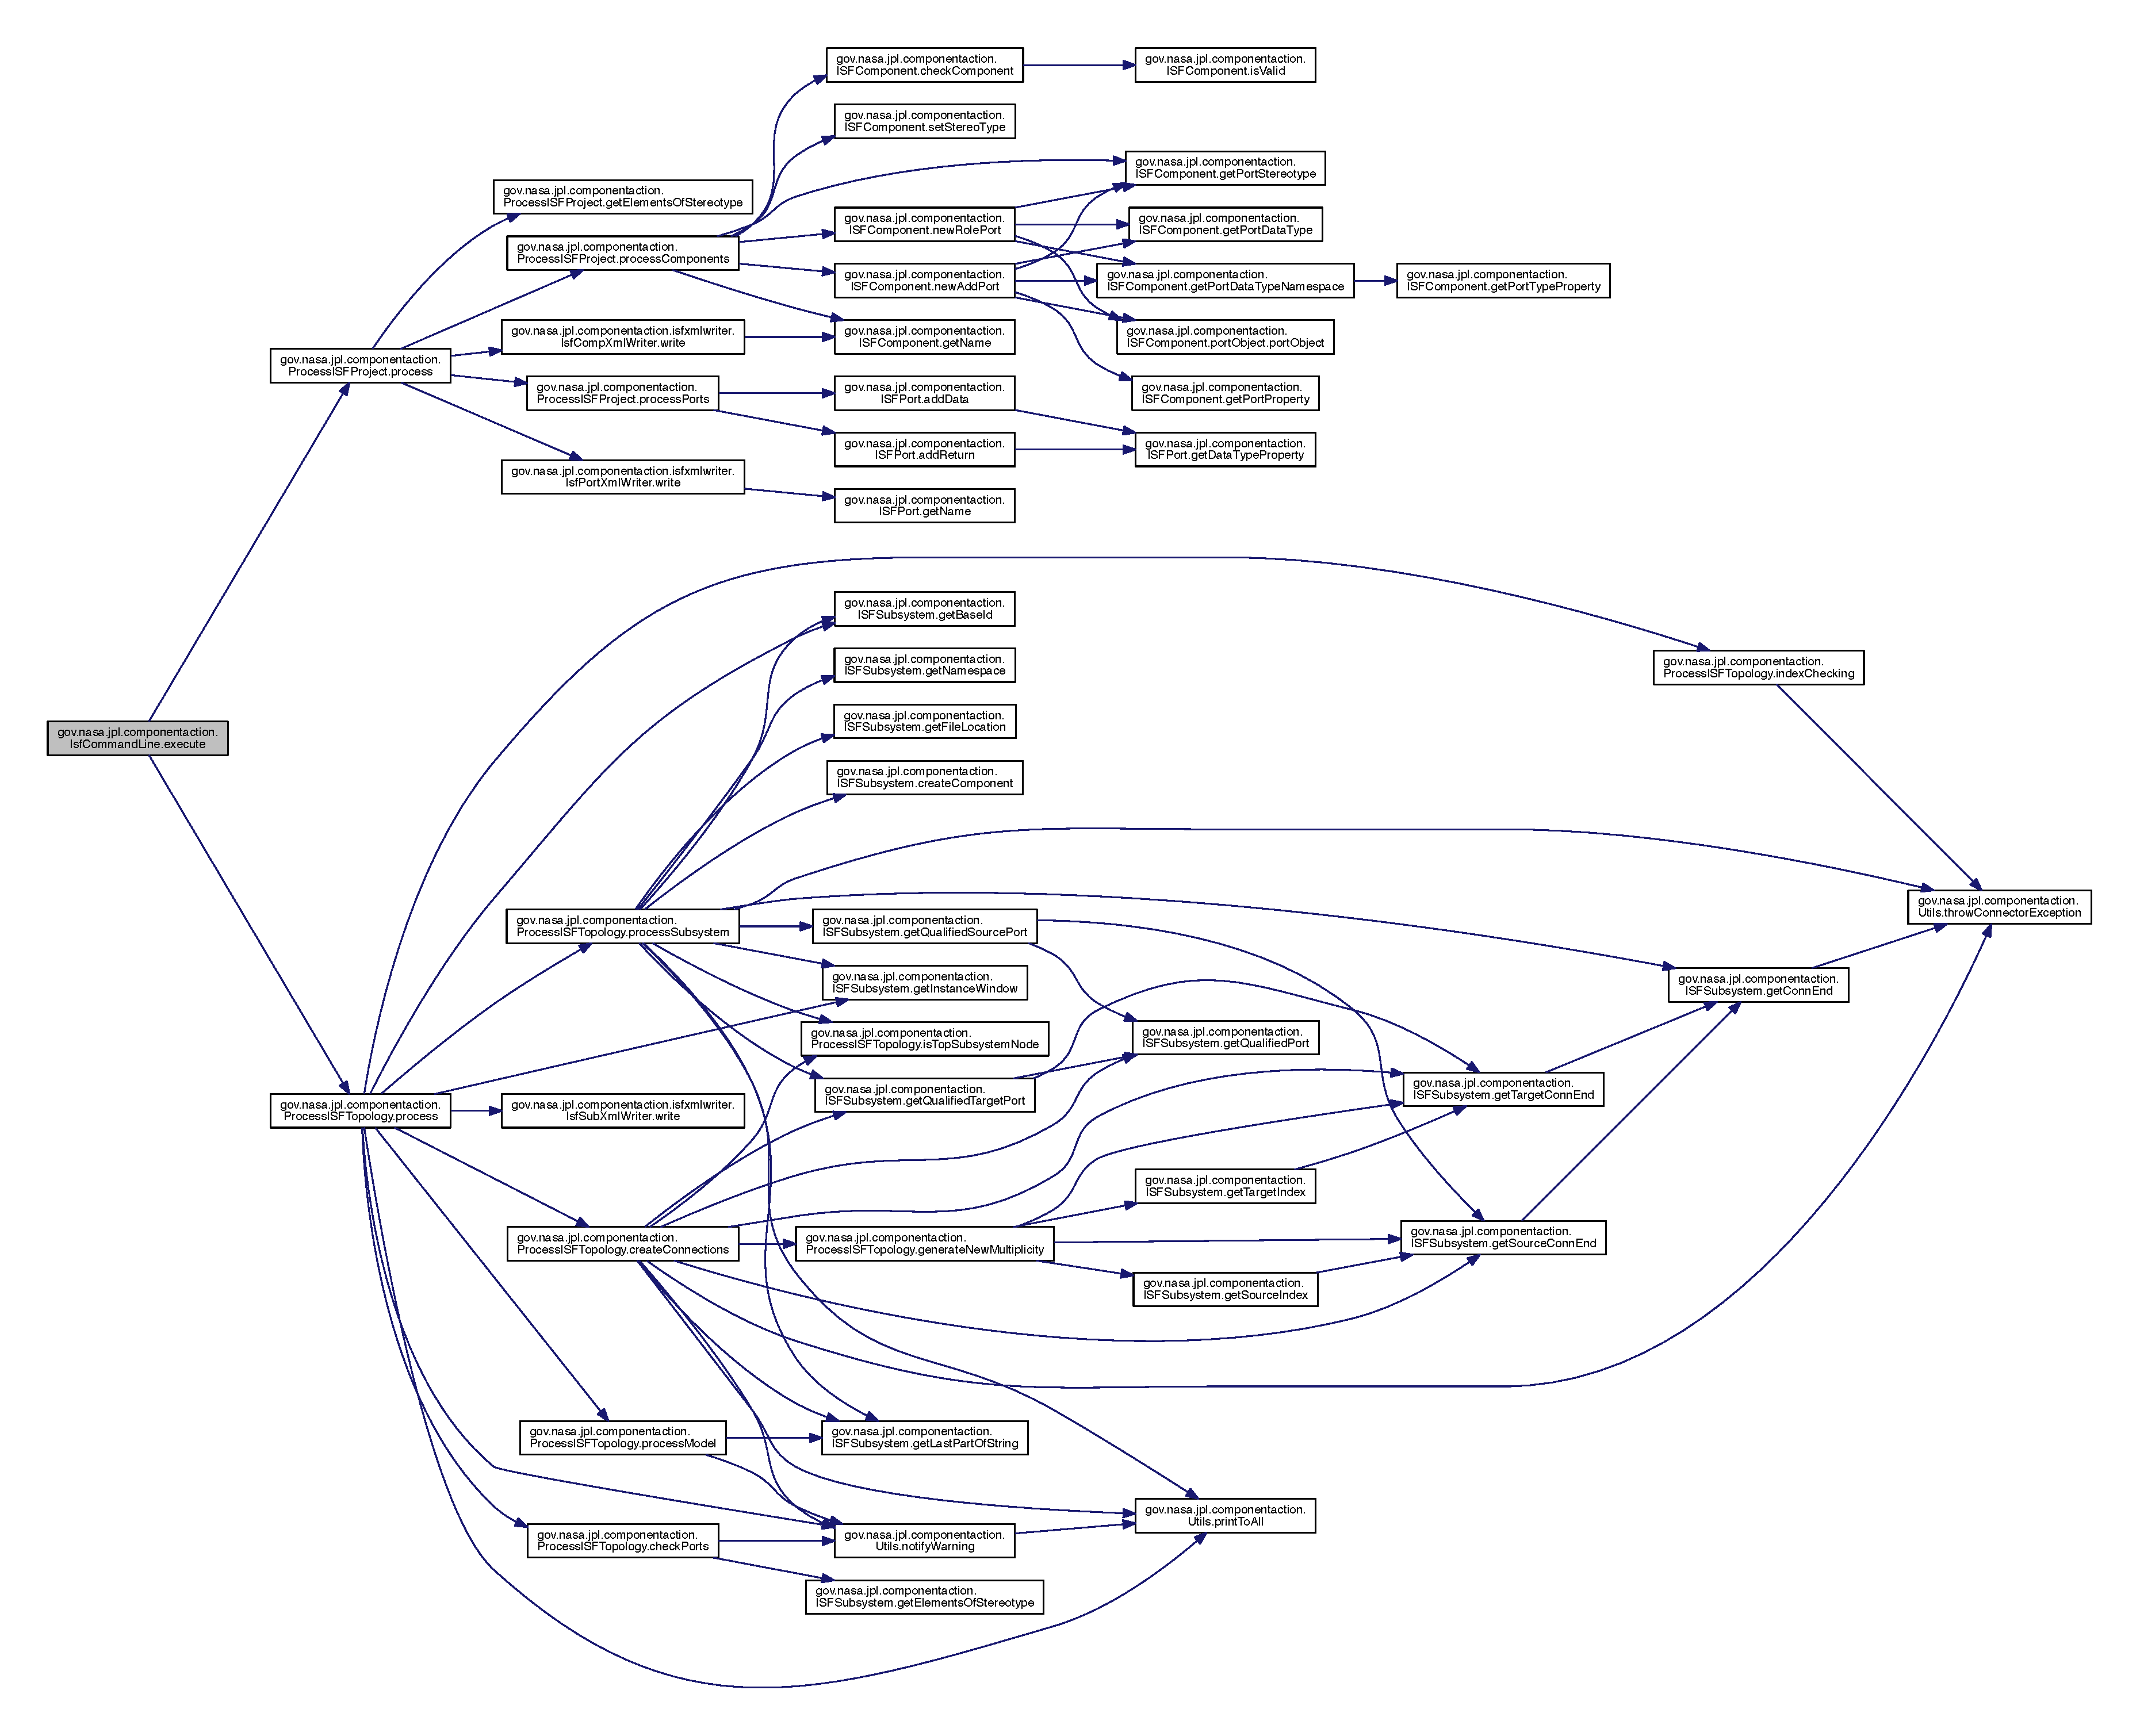
\includegraphics[width=350pt]{classgov_1_1nasa_1_1jpl_1_1componentaction_1_1_isf_command_line_ae4b2178b8721a8ec817fc16c75613b99_cgraph}
\end{center}
\end{figure}


\index{gov\+::nasa\+::jpl\+::componentaction\+::\+Isf\+Command\+Line@{gov\+::nasa\+::jpl\+::componentaction\+::\+Isf\+Command\+Line}!main@{main}}
\index{main@{main}!gov\+::nasa\+::jpl\+::componentaction\+::\+Isf\+Command\+Line@{gov\+::nasa\+::jpl\+::componentaction\+::\+Isf\+Command\+Line}}
\subsubsection[{main(\+String[] args)}]{\setlength{\rightskip}{0pt plus 5cm}static void gov.\+nasa.\+jpl.\+componentaction.\+Isf\+Command\+Line.\+main (
\begin{DoxyParamCaption}
\item[{String[$\,$]}]{args}
\end{DoxyParamCaption}
)\hspace{0.3cm}{\ttfamily [static]}}\label{classgov_1_1nasa_1_1jpl_1_1componentaction_1_1_isf_command_line_a87d3ce76d79fbf0dbd58a23ef2b8477c}
Reads the command line arguments and launches the program


\begin{DoxyParams}{Parameters}
{\em args} & application arguments. \\
\hline
\end{DoxyParams}


\subsection{Member Data Documentation}
\index{gov\+::nasa\+::jpl\+::componentaction\+::\+Isf\+Command\+Line@{gov\+::nasa\+::jpl\+::componentaction\+::\+Isf\+Command\+Line}!C\+O\+P\+Y\+R\+I\+G\+HT@{C\+O\+P\+Y\+R\+I\+G\+HT}}
\index{C\+O\+P\+Y\+R\+I\+G\+HT@{C\+O\+P\+Y\+R\+I\+G\+HT}!gov\+::nasa\+::jpl\+::componentaction\+::\+Isf\+Command\+Line@{gov\+::nasa\+::jpl\+::componentaction\+::\+Isf\+Command\+Line}}
\subsubsection[{C\+O\+P\+Y\+R\+I\+G\+HT}]{\setlength{\rightskip}{0pt plus 5cm}final String gov.\+nasa.\+jpl.\+componentaction.\+Isf\+Command\+Line.\+C\+O\+P\+Y\+R\+I\+G\+HT = \char`\"{}Copyright 2015 (California Institute of Technology)\textbackslash{}n\+A\+LL R\+I\+G\+H\+TS R\+E\+S\+E\+R\+V\+E\+D. U.\+S. Government Sponsorship acknowledged.\char`\"{}\hspace{0.3cm}{\ttfamily [static]}, {\ttfamily [private]}}\label{classgov_1_1nasa_1_1jpl_1_1componentaction_1_1_isf_command_line_a0bf1e7c43bf5d249775cf3934e1f1091}
\index{gov\+::nasa\+::jpl\+::componentaction\+::\+Isf\+Command\+Line@{gov\+::nasa\+::jpl\+::componentaction\+::\+Isf\+Command\+Line}!P\+A\+C\+K\+A\+GE@{P\+A\+C\+K\+A\+GE}}
\index{P\+A\+C\+K\+A\+GE@{P\+A\+C\+K\+A\+GE}!gov\+::nasa\+::jpl\+::componentaction\+::\+Isf\+Command\+Line@{gov\+::nasa\+::jpl\+::componentaction\+::\+Isf\+Command\+Line}}
\subsubsection[{P\+A\+C\+K\+A\+GE}]{\setlength{\rightskip}{0pt plus 5cm}final String gov.\+nasa.\+jpl.\+componentaction.\+Isf\+Command\+Line.\+P\+A\+C\+K\+A\+GE = \char`\"{}package\char`\"{}\hspace{0.3cm}{\ttfamily [static]}, {\ttfamily [private]}}\label{classgov_1_1nasa_1_1jpl_1_1componentaction_1_1_isf_command_line_a9f56a80982900571a406549313523f1b}
\index{gov\+::nasa\+::jpl\+::componentaction\+::\+Isf\+Command\+Line@{gov\+::nasa\+::jpl\+::componentaction\+::\+Isf\+Command\+Line}!plugin\+Dir@{plugin\+Dir}}
\index{plugin\+Dir@{plugin\+Dir}!gov\+::nasa\+::jpl\+::componentaction\+::\+Isf\+Command\+Line@{gov\+::nasa\+::jpl\+::componentaction\+::\+Isf\+Command\+Line}}
\subsubsection[{plugin\+Dir}]{\setlength{\rightskip}{0pt plus 5cm}File gov.\+nasa.\+jpl.\+componentaction.\+Isf\+Command\+Line.\+plugin\+Dir\hspace{0.3cm}{\ttfamily [static]}, {\ttfamily [package]}}\label{classgov_1_1nasa_1_1jpl_1_1componentaction_1_1_isf_command_line_aef1b992439a1c48f8ba4261c988fcbef}
\index{gov\+::nasa\+::jpl\+::componentaction\+::\+Isf\+Command\+Line@{gov\+::nasa\+::jpl\+::componentaction\+::\+Isf\+Command\+Line}!P\+R\+O\+J\+E\+CT@{P\+R\+O\+J\+E\+CT}}
\index{P\+R\+O\+J\+E\+CT@{P\+R\+O\+J\+E\+CT}!gov\+::nasa\+::jpl\+::componentaction\+::\+Isf\+Command\+Line@{gov\+::nasa\+::jpl\+::componentaction\+::\+Isf\+Command\+Line}}
\subsubsection[{P\+R\+O\+J\+E\+CT}]{\setlength{\rightskip}{0pt plus 5cm}final String gov.\+nasa.\+jpl.\+componentaction.\+Isf\+Command\+Line.\+P\+R\+O\+J\+E\+CT = \char`\"{}project\+\_\+name\char`\"{}\hspace{0.3cm}{\ttfamily [static]}, {\ttfamily [private]}}\label{classgov_1_1nasa_1_1jpl_1_1componentaction_1_1_isf_command_line_a0b3be7f1d37d272edb4f299059450232}
\index{gov\+::nasa\+::jpl\+::componentaction\+::\+Isf\+Command\+Line@{gov\+::nasa\+::jpl\+::componentaction\+::\+Isf\+Command\+Line}!project\+File@{project\+File}}
\index{project\+File@{project\+File}!gov\+::nasa\+::jpl\+::componentaction\+::\+Isf\+Command\+Line@{gov\+::nasa\+::jpl\+::componentaction\+::\+Isf\+Command\+Line}}
\subsubsection[{project\+File}]{\setlength{\rightskip}{0pt plus 5cm}String gov.\+nasa.\+jpl.\+componentaction.\+Isf\+Command\+Line.\+project\+File\hspace{0.3cm}{\ttfamily [static]}, {\ttfamily [package]}}\label{classgov_1_1nasa_1_1jpl_1_1componentaction_1_1_isf_command_line_a129160a912385063acbf5a084a10490a}
\index{gov\+::nasa\+::jpl\+::componentaction\+::\+Isf\+Command\+Line@{gov\+::nasa\+::jpl\+::componentaction\+::\+Isf\+Command\+Line}!U\+S\+A\+GE@{U\+S\+A\+GE}}
\index{U\+S\+A\+GE@{U\+S\+A\+GE}!gov\+::nasa\+::jpl\+::componentaction\+::\+Isf\+Command\+Line@{gov\+::nasa\+::jpl\+::componentaction\+::\+Isf\+Command\+Line}}
\subsubsection[{U\+S\+A\+GE}]{\setlength{\rightskip}{0pt plus 5cm}final String gov.\+nasa.\+jpl.\+componentaction.\+Isf\+Command\+Line.\+U\+S\+A\+GE = \char`\"{}isfpluginexec [options]\textbackslash{}n\+Before running on headless environment, use Xvfb to set up a virtual X11 display server\textbackslash{}n/usr/bin/Xvfb \+:1 -\/screen 0 1024x768x24\textbackslash{}nexport D\+I\+S\+P\+L\+A\+Y=\+:1\char`\"{}\hspace{0.3cm}{\ttfamily [static]}, {\ttfamily [private]}}\label{classgov_1_1nasa_1_1jpl_1_1componentaction_1_1_isf_command_line_a39d9a0269d69c1b26dc9878902ad698c}


The documentation for this class was generated from the following file\+:\begin{DoxyCompactItemize}
\item 
src/gov/nasa/jpl/componentaction/{\bf Isf\+Command\+Line.\+java}\end{DoxyCompactItemize}

\section{gov.\+nasa.\+jpl.\+componentaction.\+I\+S\+F\+Component Class Reference}
\label{classgov_1_1nasa_1_1jpl_1_1componentaction_1_1_i_s_f_component}\index{gov.\+nasa.\+jpl.\+componentaction.\+I\+S\+F\+Component@{gov.\+nasa.\+jpl.\+componentaction.\+I\+S\+F\+Component}}


Collaboration diagram for gov.\+nasa.\+jpl.\+componentaction.\+I\+S\+F\+Component\+:
\nopagebreak
\begin{figure}[H]
\begin{center}
\leavevmode
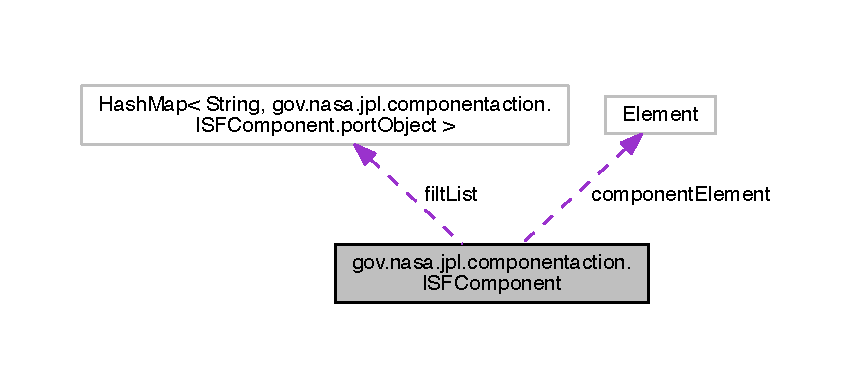
\includegraphics[width=350pt]{classgov_1_1nasa_1_1jpl_1_1componentaction_1_1_i_s_f_component__coll__graph}
\end{center}
\end{figure}
\subsection*{Classes}
\begin{DoxyCompactItemize}
\item 
class {\bf port\+Object}
\item 
class {\bf reference\+Port}
\end{DoxyCompactItemize}
\subsection*{Public Member Functions}
\begin{DoxyCompactItemize}
\item 
{\bf I\+S\+F\+Component} (Element {\bf component\+Element})
\item 
void {\bf set\+Stereo\+Type} (String {\bf comp\+Stereotype})
\item 
void {\bf new\+Add\+Port} (Element port\+Element)  throws Port\+Exception 
\item 
void {\bf new\+Role\+Port} (Element port\+Element)  throws Port\+Exception 
\item 
String {\bf get\+Port\+Name} (Element port\+Element)
\item 
String {\bf get\+Port\+Stereotype} (Element port\+Element)
\item 
String {\bf get\+Port\+Data\+Type} (Element port\+Element)  throws Port\+Exception 
\item 
String {\bf get\+Port\+Data\+Type\+Namespace} (Element port\+Element)
\item 
Hash\+Map$<$ String, {\bf port\+Object} $>$ {\bf get\+Port\+Hash\+List} ()
\item 
String {\bf get\+U\+RI} ()
\item 
String {\bf get\+Include\+Cmd\+X\+ML} ()
\item 
String {\bf get\+Include\+Evr\+X\+ML} ()
\item 
String {\bf get\+Include\+Tlm\+X\+ML} ()
\item 
String {\bf get\+Include\+Param\+X\+ML} ()
\item 
String {\bf get\+Include\+Internal\+I\+F\+X\+ML} ()
\item 
String {\bf get\+Include\+Hdr\+File} ()
\item 
String {\bf get\+Namespace} ()
\item 
String {\bf get\+Name} ()
\item 
String {\bf get\+Stereotype} ()
\item 
List$<$ String $>$ {\bf get\+Port\+Data\+List} ()
\item 
String {\bf get\+Port\+Type\+Property} (Element port\+Element, String property)
\item 
String {\bf get\+Component\+Property} (Element port\+Element, String property)
\item 
String {\bf get\+Port\+Property} (Element port\+Element, String property)
\item 
void {\bf print} ()
\item 
void {\bf check\+Component} ()  throws Component\+Exception 
\item 
void {\bf warn\+Log} (String err\+Str)
\item 
boolean {\bf is\+Valid} (String stereotype, String port\+Type, boolean at\+Least\+One)
\end{DoxyCompactItemize}
\subsection*{Package Attributes}
\begin{DoxyCompactItemize}
\item 
Hash\+Map$<$ String, {\bf port\+Object} $>$ {\bf filt\+List}
\item 
String {\bf Include\+Cmd\+X\+ML}
\item 
String {\bf Include\+Tlm\+X\+ML}
\item 
String {\bf Include\+Evr\+X\+ML}
\item 
String {\bf Include\+Param\+X\+ML}
\item 
String {\bf Include\+Internal\+I\+F\+X\+ML}
\item 
String {\bf Include\+Include\+Hdr}
\end{DoxyCompactItemize}
\subsection*{Private Member Functions}
\begin{DoxyCompactItemize}
\item 
String {\bf get\+Dictionary\+String} (String include\+String)
\end{DoxyCompactItemize}
\subsection*{Private Attributes}
\begin{DoxyCompactItemize}
\item 
Element {\bf component\+Element}
\item 
String {\bf comp\+Stereotype}
\item 
String {\bf U\+R\+I\+Name}
\end{DoxyCompactItemize}


\subsection{Detailed Description}
This class encapsulates information pertaining to the component types and their ports in the MD model -\/ ie active, passive or queued components 

\subsection{Constructor \& Destructor Documentation}
\index{gov\+::nasa\+::jpl\+::componentaction\+::\+I\+S\+F\+Component@{gov\+::nasa\+::jpl\+::componentaction\+::\+I\+S\+F\+Component}!I\+S\+F\+Component@{I\+S\+F\+Component}}
\index{I\+S\+F\+Component@{I\+S\+F\+Component}!gov\+::nasa\+::jpl\+::componentaction\+::\+I\+S\+F\+Component@{gov\+::nasa\+::jpl\+::componentaction\+::\+I\+S\+F\+Component}}
\subsubsection[{I\+S\+F\+Component(\+Element component\+Element)}]{\setlength{\rightskip}{0pt plus 5cm}gov.\+nasa.\+jpl.\+componentaction.\+I\+S\+F\+Component.\+I\+S\+F\+Component (
\begin{DoxyParamCaption}
\item[{Element}]{component\+Element}
\end{DoxyParamCaption}
)}\label{classgov_1_1nasa_1_1jpl_1_1componentaction_1_1_i_s_f_component_af898760279b1ccfb50f0edd62a3bc178}
Instantiation for the \doxyref{I\+S\+F\+Component}{p.}{classgov_1_1nasa_1_1jpl_1_1componentaction_1_1_i_s_f_component}.


\begin{DoxyParams}{Parameters}
{\em component\+Element} & The element of the component that will be processed. \\
\hline
\end{DoxyParams}


Here is the call graph for this function\+:
\nopagebreak
\begin{figure}[H]
\begin{center}
\leavevmode
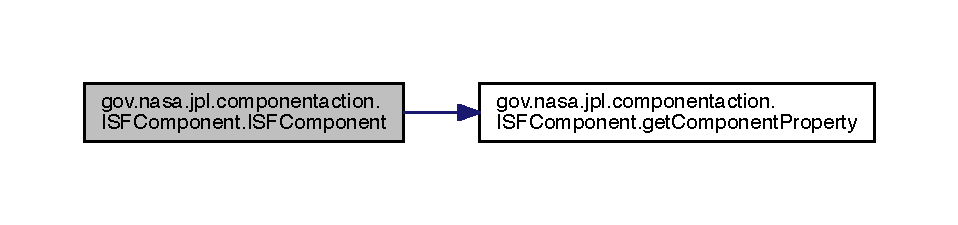
\includegraphics[width=350pt]{classgov_1_1nasa_1_1jpl_1_1componentaction_1_1_i_s_f_component_af898760279b1ccfb50f0edd62a3bc178_cgraph}
\end{center}
\end{figure}




\subsection{Member Function Documentation}
\index{gov\+::nasa\+::jpl\+::componentaction\+::\+I\+S\+F\+Component@{gov\+::nasa\+::jpl\+::componentaction\+::\+I\+S\+F\+Component}!check\+Component@{check\+Component}}
\index{check\+Component@{check\+Component}!gov\+::nasa\+::jpl\+::componentaction\+::\+I\+S\+F\+Component@{gov\+::nasa\+::jpl\+::componentaction\+::\+I\+S\+F\+Component}}
\subsubsection[{check\+Component()}]{\setlength{\rightskip}{0pt plus 5cm}void gov.\+nasa.\+jpl.\+componentaction.\+I\+S\+F\+Component.\+check\+Component (
\begin{DoxyParamCaption}
{}
\end{DoxyParamCaption}
) throws {\bf Component\+Exception}}\label{classgov_1_1nasa_1_1jpl_1_1componentaction_1_1_i_s_f_component_a871d690c6c099aff73a4f307d17ce1bd}
All passive components cannot have async\+\_\+input ports All active components should have sync\+\_\+input ports All queued components should have sync and async input ports 
\begin{DoxyExceptions}{Exceptions}
{\em \doxyref{Component\+Exception}{p.}{classgov_1_1nasa_1_1jpl_1_1componentaction_1_1_component_exception}} & \\
\hline
\end{DoxyExceptions}


Here is the call graph for this function\+:
\nopagebreak
\begin{figure}[H]
\begin{center}
\leavevmode
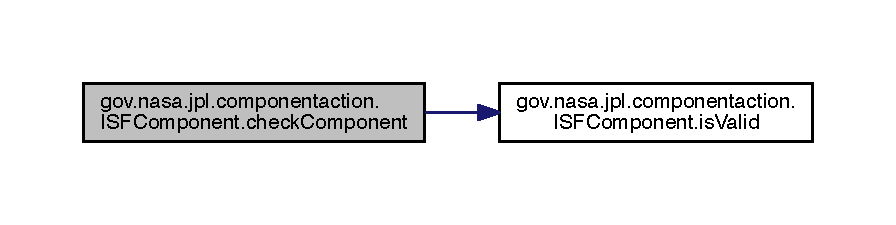
\includegraphics[width=350pt]{classgov_1_1nasa_1_1jpl_1_1componentaction_1_1_i_s_f_component_a871d690c6c099aff73a4f307d17ce1bd_cgraph}
\end{center}
\end{figure}




Here is the caller graph for this function\+:
\nopagebreak
\begin{figure}[H]
\begin{center}
\leavevmode
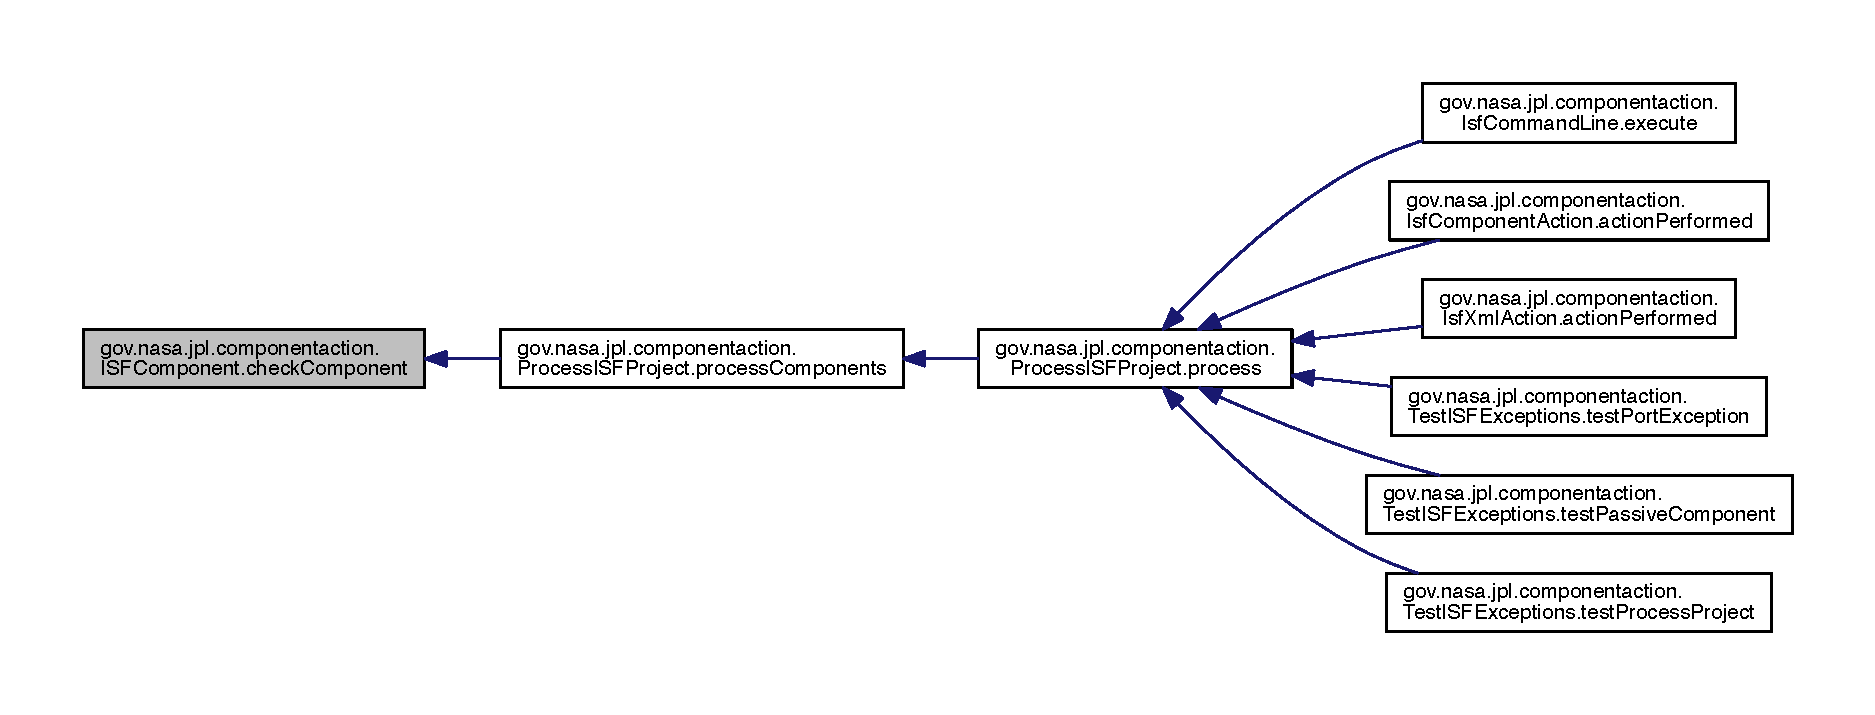
\includegraphics[width=350pt]{classgov_1_1nasa_1_1jpl_1_1componentaction_1_1_i_s_f_component_a871d690c6c099aff73a4f307d17ce1bd_icgraph}
\end{center}
\end{figure}


\index{gov\+::nasa\+::jpl\+::componentaction\+::\+I\+S\+F\+Component@{gov\+::nasa\+::jpl\+::componentaction\+::\+I\+S\+F\+Component}!get\+Component\+Property@{get\+Component\+Property}}
\index{get\+Component\+Property@{get\+Component\+Property}!gov\+::nasa\+::jpl\+::componentaction\+::\+I\+S\+F\+Component@{gov\+::nasa\+::jpl\+::componentaction\+::\+I\+S\+F\+Component}}
\subsubsection[{get\+Component\+Property(\+Element port\+Element, String property)}]{\setlength{\rightskip}{0pt plus 5cm}String gov.\+nasa.\+jpl.\+componentaction.\+I\+S\+F\+Component.\+get\+Component\+Property (
\begin{DoxyParamCaption}
\item[{Element}]{port\+Element, }
\item[{String}]{property}
\end{DoxyParamCaption}
)}\label{classgov_1_1nasa_1_1jpl_1_1componentaction_1_1_i_s_f_component_a37eb712a125aa28b10b9197e3316c6dd}
Returns the property value of Component stereotype of the input element argument. 
\begin{DoxyParams}{Parameters}
{\em port\+Element} & Element of the port type \\
\hline
{\em property} & String of value to be looked for in the stereotype Component \\
\hline
\end{DoxyParams}
\begin{DoxyReturn}{Returns}
The value of the attribute from property 
\end{DoxyReturn}


Here is the caller graph for this function\+:
\nopagebreak
\begin{figure}[H]
\begin{center}
\leavevmode
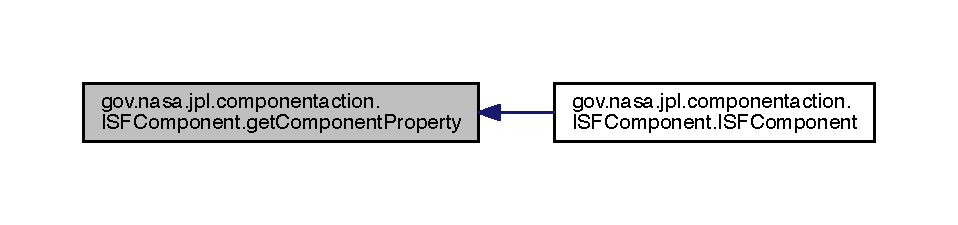
\includegraphics[width=350pt]{classgov_1_1nasa_1_1jpl_1_1componentaction_1_1_i_s_f_component_a37eb712a125aa28b10b9197e3316c6dd_icgraph}
\end{center}
\end{figure}


\index{gov\+::nasa\+::jpl\+::componentaction\+::\+I\+S\+F\+Component@{gov\+::nasa\+::jpl\+::componentaction\+::\+I\+S\+F\+Component}!get\+Dictionary\+String@{get\+Dictionary\+String}}
\index{get\+Dictionary\+String@{get\+Dictionary\+String}!gov\+::nasa\+::jpl\+::componentaction\+::\+I\+S\+F\+Component@{gov\+::nasa\+::jpl\+::componentaction\+::\+I\+S\+F\+Component}}
\subsubsection[{get\+Dictionary\+String(\+String include\+String)}]{\setlength{\rightskip}{0pt plus 5cm}String gov.\+nasa.\+jpl.\+componentaction.\+I\+S\+F\+Component.\+get\+Dictionary\+String (
\begin{DoxyParamCaption}
\item[{String}]{include\+String}
\end{DoxyParamCaption}
)\hspace{0.3cm}{\ttfamily [private]}}\label{classgov_1_1nasa_1_1jpl_1_1componentaction_1_1_i_s_f_component_a36ed8a30e3c8709b0a56743d9db5e1fa}
Return the full dictionary path which includes the U\+RI path specified in the package above the component. 
\begin{DoxyParams}{Parameters}
{\em include\+String} & \\
\hline
\end{DoxyParams}
\begin{DoxyReturn}{Returns}
input string prepended by U\+R\+I\+Name 
\end{DoxyReturn}


Here is the caller graph for this function\+:
\nopagebreak
\begin{figure}[H]
\begin{center}
\leavevmode
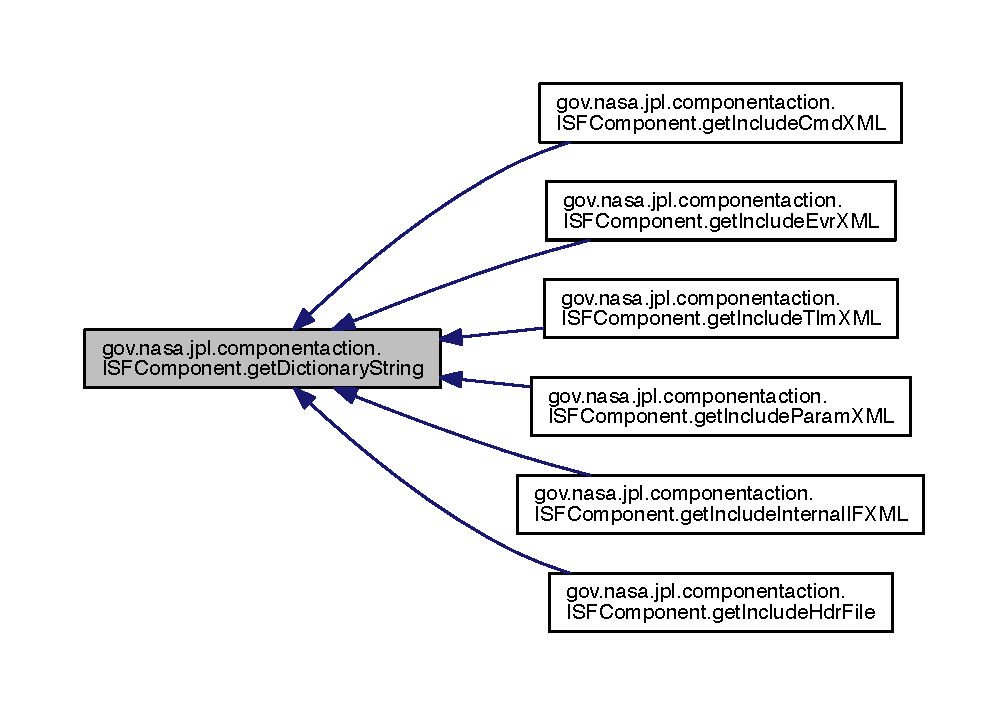
\includegraphics[width=350pt]{classgov_1_1nasa_1_1jpl_1_1componentaction_1_1_i_s_f_component_a36ed8a30e3c8709b0a56743d9db5e1fa_icgraph}
\end{center}
\end{figure}


\index{gov\+::nasa\+::jpl\+::componentaction\+::\+I\+S\+F\+Component@{gov\+::nasa\+::jpl\+::componentaction\+::\+I\+S\+F\+Component}!get\+Include\+Cmd\+X\+ML@{get\+Include\+Cmd\+X\+ML}}
\index{get\+Include\+Cmd\+X\+ML@{get\+Include\+Cmd\+X\+ML}!gov\+::nasa\+::jpl\+::componentaction\+::\+I\+S\+F\+Component@{gov\+::nasa\+::jpl\+::componentaction\+::\+I\+S\+F\+Component}}
\subsubsection[{get\+Include\+Cmd\+X\+M\+L()}]{\setlength{\rightskip}{0pt plus 5cm}String gov.\+nasa.\+jpl.\+componentaction.\+I\+S\+F\+Component.\+get\+Include\+Cmd\+X\+ML (
\begin{DoxyParamCaption}
{}
\end{DoxyParamCaption}
)}\label{classgov_1_1nasa_1_1jpl_1_1componentaction_1_1_i_s_f_component_af0727ee60b09fdf3a0716d589d918a7b}
Prepends the Include\+Cmd\+X\+ML String with the U\+RI Name \begin{DoxyReturn}{Returns}
address string 
\end{DoxyReturn}


Here is the call graph for this function\+:
\nopagebreak
\begin{figure}[H]
\begin{center}
\leavevmode
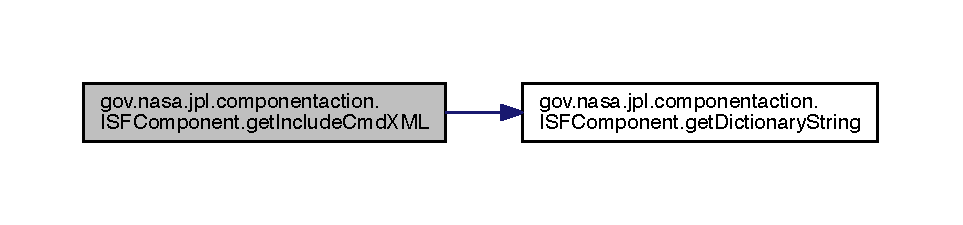
\includegraphics[width=350pt]{classgov_1_1nasa_1_1jpl_1_1componentaction_1_1_i_s_f_component_af0727ee60b09fdf3a0716d589d918a7b_cgraph}
\end{center}
\end{figure}


\index{gov\+::nasa\+::jpl\+::componentaction\+::\+I\+S\+F\+Component@{gov\+::nasa\+::jpl\+::componentaction\+::\+I\+S\+F\+Component}!get\+Include\+Evr\+X\+ML@{get\+Include\+Evr\+X\+ML}}
\index{get\+Include\+Evr\+X\+ML@{get\+Include\+Evr\+X\+ML}!gov\+::nasa\+::jpl\+::componentaction\+::\+I\+S\+F\+Component@{gov\+::nasa\+::jpl\+::componentaction\+::\+I\+S\+F\+Component}}
\subsubsection[{get\+Include\+Evr\+X\+M\+L()}]{\setlength{\rightskip}{0pt plus 5cm}String gov.\+nasa.\+jpl.\+componentaction.\+I\+S\+F\+Component.\+get\+Include\+Evr\+X\+ML (
\begin{DoxyParamCaption}
{}
\end{DoxyParamCaption}
)}\label{classgov_1_1nasa_1_1jpl_1_1componentaction_1_1_i_s_f_component_a8f55c8b2e58e0ed273a5ace89d12b667}
Prepends the Include\+Evr\+X\+ML String with the U\+RI Name \begin{DoxyReturn}{Returns}
address string 
\end{DoxyReturn}


Here is the call graph for this function\+:
\nopagebreak
\begin{figure}[H]
\begin{center}
\leavevmode
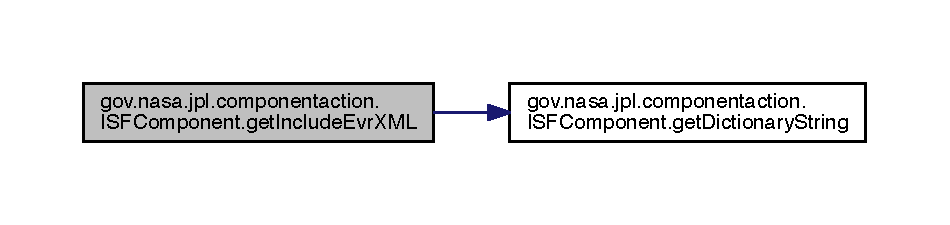
\includegraphics[width=350pt]{classgov_1_1nasa_1_1jpl_1_1componentaction_1_1_i_s_f_component_a8f55c8b2e58e0ed273a5ace89d12b667_cgraph}
\end{center}
\end{figure}


\index{gov\+::nasa\+::jpl\+::componentaction\+::\+I\+S\+F\+Component@{gov\+::nasa\+::jpl\+::componentaction\+::\+I\+S\+F\+Component}!get\+Include\+Hdr\+File@{get\+Include\+Hdr\+File}}
\index{get\+Include\+Hdr\+File@{get\+Include\+Hdr\+File}!gov\+::nasa\+::jpl\+::componentaction\+::\+I\+S\+F\+Component@{gov\+::nasa\+::jpl\+::componentaction\+::\+I\+S\+F\+Component}}
\subsubsection[{get\+Include\+Hdr\+File()}]{\setlength{\rightskip}{0pt plus 5cm}String gov.\+nasa.\+jpl.\+componentaction.\+I\+S\+F\+Component.\+get\+Include\+Hdr\+File (
\begin{DoxyParamCaption}
{}
\end{DoxyParamCaption}
)}\label{classgov_1_1nasa_1_1jpl_1_1componentaction_1_1_i_s_f_component_a641df5cf88a85773d7d852dbfe043751}
Prepends the Include\+Include\+Hdr String with the U\+RI Name \begin{DoxyReturn}{Returns}
address string 
\end{DoxyReturn}


Here is the call graph for this function\+:
\nopagebreak
\begin{figure}[H]
\begin{center}
\leavevmode
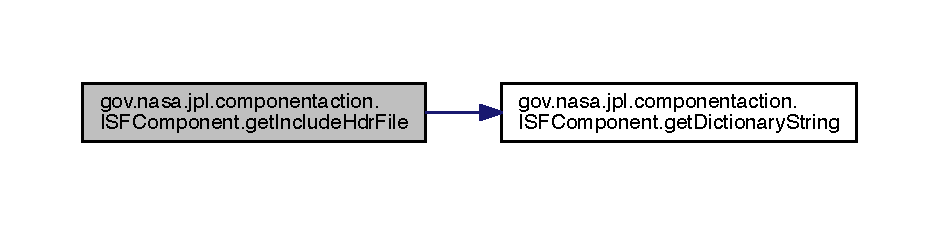
\includegraphics[width=350pt]{classgov_1_1nasa_1_1jpl_1_1componentaction_1_1_i_s_f_component_a641df5cf88a85773d7d852dbfe043751_cgraph}
\end{center}
\end{figure}


\index{gov\+::nasa\+::jpl\+::componentaction\+::\+I\+S\+F\+Component@{gov\+::nasa\+::jpl\+::componentaction\+::\+I\+S\+F\+Component}!get\+Include\+Internal\+I\+F\+X\+ML@{get\+Include\+Internal\+I\+F\+X\+ML}}
\index{get\+Include\+Internal\+I\+F\+X\+ML@{get\+Include\+Internal\+I\+F\+X\+ML}!gov\+::nasa\+::jpl\+::componentaction\+::\+I\+S\+F\+Component@{gov\+::nasa\+::jpl\+::componentaction\+::\+I\+S\+F\+Component}}
\subsubsection[{get\+Include\+Internal\+I\+F\+X\+M\+L()}]{\setlength{\rightskip}{0pt plus 5cm}String gov.\+nasa.\+jpl.\+componentaction.\+I\+S\+F\+Component.\+get\+Include\+Internal\+I\+F\+X\+ML (
\begin{DoxyParamCaption}
{}
\end{DoxyParamCaption}
)}\label{classgov_1_1nasa_1_1jpl_1_1componentaction_1_1_i_s_f_component_a752ce972eb48aac1d34c297250938e87}
Prepends the Include\+Internal\+I\+F\+X\+ML String with the U\+RI Name \begin{DoxyReturn}{Returns}
address string 
\end{DoxyReturn}


Here is the call graph for this function\+:
\nopagebreak
\begin{figure}[H]
\begin{center}
\leavevmode
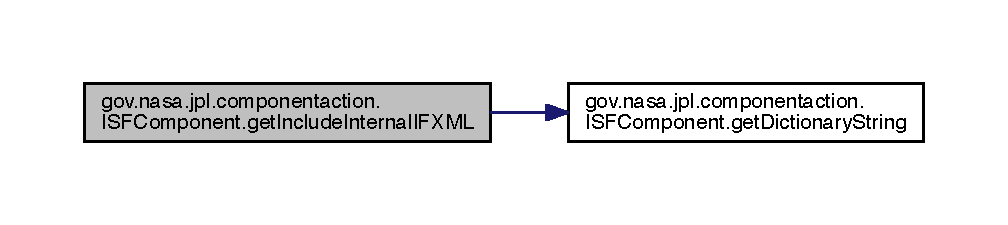
\includegraphics[width=350pt]{classgov_1_1nasa_1_1jpl_1_1componentaction_1_1_i_s_f_component_a752ce972eb48aac1d34c297250938e87_cgraph}
\end{center}
\end{figure}


\index{gov\+::nasa\+::jpl\+::componentaction\+::\+I\+S\+F\+Component@{gov\+::nasa\+::jpl\+::componentaction\+::\+I\+S\+F\+Component}!get\+Include\+Param\+X\+ML@{get\+Include\+Param\+X\+ML}}
\index{get\+Include\+Param\+X\+ML@{get\+Include\+Param\+X\+ML}!gov\+::nasa\+::jpl\+::componentaction\+::\+I\+S\+F\+Component@{gov\+::nasa\+::jpl\+::componentaction\+::\+I\+S\+F\+Component}}
\subsubsection[{get\+Include\+Param\+X\+M\+L()}]{\setlength{\rightskip}{0pt plus 5cm}String gov.\+nasa.\+jpl.\+componentaction.\+I\+S\+F\+Component.\+get\+Include\+Param\+X\+ML (
\begin{DoxyParamCaption}
{}
\end{DoxyParamCaption}
)}\label{classgov_1_1nasa_1_1jpl_1_1componentaction_1_1_i_s_f_component_a769e07641248e4fe00b5e4822d8d335a}
Prepends the Include\+Param\+X\+ML String with the U\+RI Name \begin{DoxyReturn}{Returns}
address string 
\end{DoxyReturn}


Here is the call graph for this function\+:
\nopagebreak
\begin{figure}[H]
\begin{center}
\leavevmode
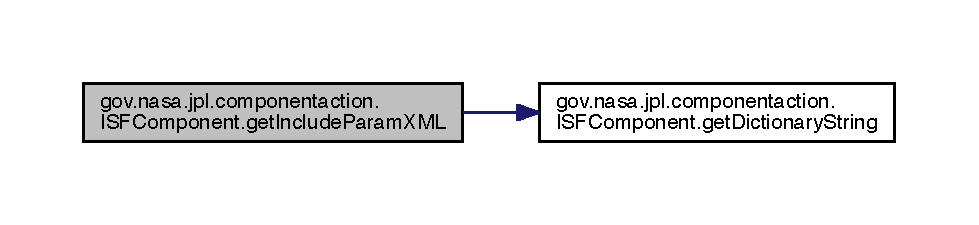
\includegraphics[width=350pt]{classgov_1_1nasa_1_1jpl_1_1componentaction_1_1_i_s_f_component_a769e07641248e4fe00b5e4822d8d335a_cgraph}
\end{center}
\end{figure}


\index{gov\+::nasa\+::jpl\+::componentaction\+::\+I\+S\+F\+Component@{gov\+::nasa\+::jpl\+::componentaction\+::\+I\+S\+F\+Component}!get\+Include\+Tlm\+X\+ML@{get\+Include\+Tlm\+X\+ML}}
\index{get\+Include\+Tlm\+X\+ML@{get\+Include\+Tlm\+X\+ML}!gov\+::nasa\+::jpl\+::componentaction\+::\+I\+S\+F\+Component@{gov\+::nasa\+::jpl\+::componentaction\+::\+I\+S\+F\+Component}}
\subsubsection[{get\+Include\+Tlm\+X\+M\+L()}]{\setlength{\rightskip}{0pt plus 5cm}String gov.\+nasa.\+jpl.\+componentaction.\+I\+S\+F\+Component.\+get\+Include\+Tlm\+X\+ML (
\begin{DoxyParamCaption}
{}
\end{DoxyParamCaption}
)}\label{classgov_1_1nasa_1_1jpl_1_1componentaction_1_1_i_s_f_component_a611e4d69970d6119504c51bb7b88006a}
Prepends the Include\+Tlm\+X\+ML String with the U\+RI Name \begin{DoxyReturn}{Returns}
address string 
\end{DoxyReturn}


Here is the call graph for this function\+:
\nopagebreak
\begin{figure}[H]
\begin{center}
\leavevmode
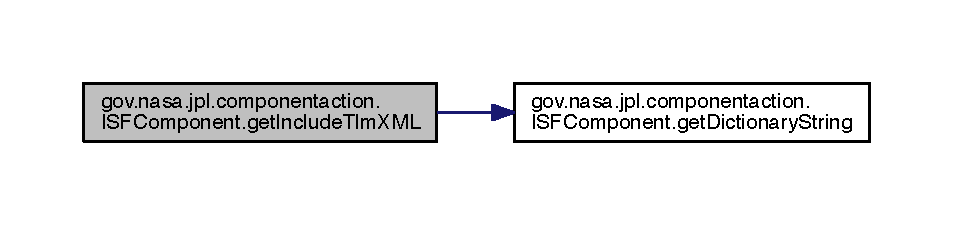
\includegraphics[width=350pt]{classgov_1_1nasa_1_1jpl_1_1componentaction_1_1_i_s_f_component_a611e4d69970d6119504c51bb7b88006a_cgraph}
\end{center}
\end{figure}


\index{gov\+::nasa\+::jpl\+::componentaction\+::\+I\+S\+F\+Component@{gov\+::nasa\+::jpl\+::componentaction\+::\+I\+S\+F\+Component}!get\+Name@{get\+Name}}
\index{get\+Name@{get\+Name}!gov\+::nasa\+::jpl\+::componentaction\+::\+I\+S\+F\+Component@{gov\+::nasa\+::jpl\+::componentaction\+::\+I\+S\+F\+Component}}
\subsubsection[{get\+Name()}]{\setlength{\rightskip}{0pt plus 5cm}String gov.\+nasa.\+jpl.\+componentaction.\+I\+S\+F\+Component.\+get\+Name (
\begin{DoxyParamCaption}
{}
\end{DoxyParamCaption}
)}\label{classgov_1_1nasa_1_1jpl_1_1componentaction_1_1_i_s_f_component_a3b3015b3b1a38b5950d80586332dc9bf}
Returns last part of the componenet\+Element name \begin{DoxyReturn}{Returns}
name 
\end{DoxyReturn}


Here is the caller graph for this function\+:
\nopagebreak
\begin{figure}[H]
\begin{center}
\leavevmode
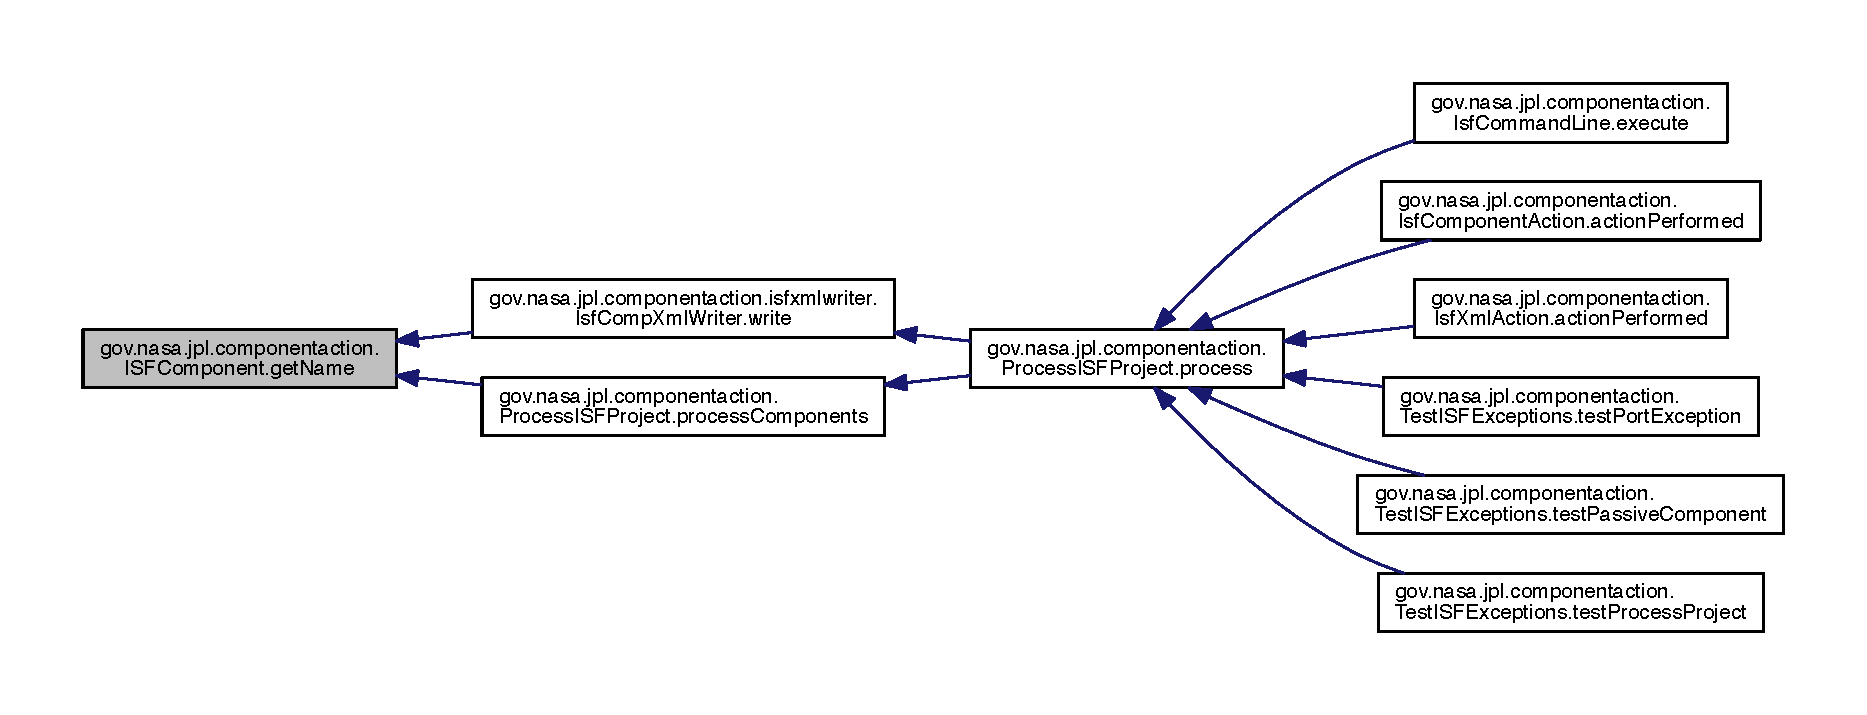
\includegraphics[width=350pt]{classgov_1_1nasa_1_1jpl_1_1componentaction_1_1_i_s_f_component_a3b3015b3b1a38b5950d80586332dc9bf_icgraph}
\end{center}
\end{figure}


\index{gov\+::nasa\+::jpl\+::componentaction\+::\+I\+S\+F\+Component@{gov\+::nasa\+::jpl\+::componentaction\+::\+I\+S\+F\+Component}!get\+Namespace@{get\+Namespace}}
\index{get\+Namespace@{get\+Namespace}!gov\+::nasa\+::jpl\+::componentaction\+::\+I\+S\+F\+Component@{gov\+::nasa\+::jpl\+::componentaction\+::\+I\+S\+F\+Component}}
\subsubsection[{get\+Namespace()}]{\setlength{\rightskip}{0pt plus 5cm}String gov.\+nasa.\+jpl.\+componentaction.\+I\+S\+F\+Component.\+get\+Namespace (
\begin{DoxyParamCaption}
{}
\end{DoxyParamCaption}
)}\label{classgov_1_1nasa_1_1jpl_1_1componentaction_1_1_i_s_f_component_a7bbbc1c208a739839c35d36557d40876}
Get the component stereotype attribute called \char`\"{}\+Namespace\char`\"{} \begin{DoxyReturn}{Returns}
Namespace string of the component\+Element 
\end{DoxyReturn}


Here is the call graph for this function\+:
\nopagebreak
\begin{figure}[H]
\begin{center}
\leavevmode
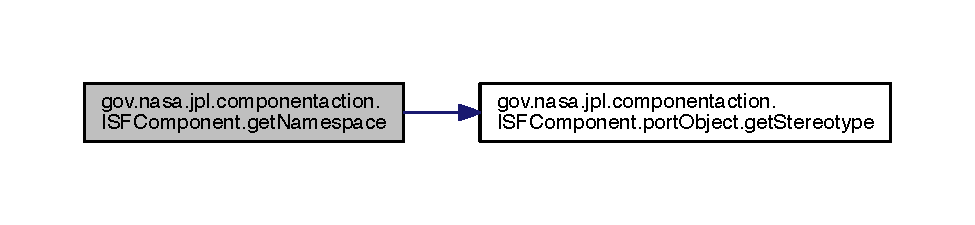
\includegraphics[width=350pt]{classgov_1_1nasa_1_1jpl_1_1componentaction_1_1_i_s_f_component_a7bbbc1c208a739839c35d36557d40876_cgraph}
\end{center}
\end{figure}


\index{gov\+::nasa\+::jpl\+::componentaction\+::\+I\+S\+F\+Component@{gov\+::nasa\+::jpl\+::componentaction\+::\+I\+S\+F\+Component}!get\+Port\+Data\+List@{get\+Port\+Data\+List}}
\index{get\+Port\+Data\+List@{get\+Port\+Data\+List}!gov\+::nasa\+::jpl\+::componentaction\+::\+I\+S\+F\+Component@{gov\+::nasa\+::jpl\+::componentaction\+::\+I\+S\+F\+Component}}
\subsubsection[{get\+Port\+Data\+List()}]{\setlength{\rightskip}{0pt plus 5cm}List$<$String$>$ gov.\+nasa.\+jpl.\+componentaction.\+I\+S\+F\+Component.\+get\+Port\+Data\+List (
\begin{DoxyParamCaption}
{}
\end{DoxyParamCaption}
)}\label{classgov_1_1nasa_1_1jpl_1_1componentaction_1_1_i_s_f_component_a72aa505f8c795f269160209c9f9b1ea6}
Creates a list of strings based off the data type from filit\+List values \begin{DoxyReturn}{Returns}
A list of data type strings 
\end{DoxyReturn}
\index{gov\+::nasa\+::jpl\+::componentaction\+::\+I\+S\+F\+Component@{gov\+::nasa\+::jpl\+::componentaction\+::\+I\+S\+F\+Component}!get\+Port\+Data\+Type@{get\+Port\+Data\+Type}}
\index{get\+Port\+Data\+Type@{get\+Port\+Data\+Type}!gov\+::nasa\+::jpl\+::componentaction\+::\+I\+S\+F\+Component@{gov\+::nasa\+::jpl\+::componentaction\+::\+I\+S\+F\+Component}}
\subsubsection[{get\+Port\+Data\+Type(\+Element port\+Element)}]{\setlength{\rightskip}{0pt plus 5cm}String gov.\+nasa.\+jpl.\+componentaction.\+I\+S\+F\+Component.\+get\+Port\+Data\+Type (
\begin{DoxyParamCaption}
\item[{Element}]{port\+Element}
\end{DoxyParamCaption}
) throws {\bf Port\+Exception}}\label{classgov_1_1nasa_1_1jpl_1_1componentaction_1_1_i_s_f_component_a18d1885312f59b16ed2a43ca059d050c}
This returns the full path of the data type which includes the directory tree.


\begin{DoxyParams}{Parameters}
{\em port\+Element} & \\
\hline
\end{DoxyParams}
\begin{DoxyReturn}{Returns}
port data type string 
\end{DoxyReturn}

\begin{DoxyExceptions}{Exceptions}
{\em \doxyref{Port\+Exception}{p.}{classgov_1_1nasa_1_1jpl_1_1componentaction_1_1_port_exception}} & \\
\hline
\end{DoxyExceptions}


Here is the caller graph for this function\+:
\nopagebreak
\begin{figure}[H]
\begin{center}
\leavevmode
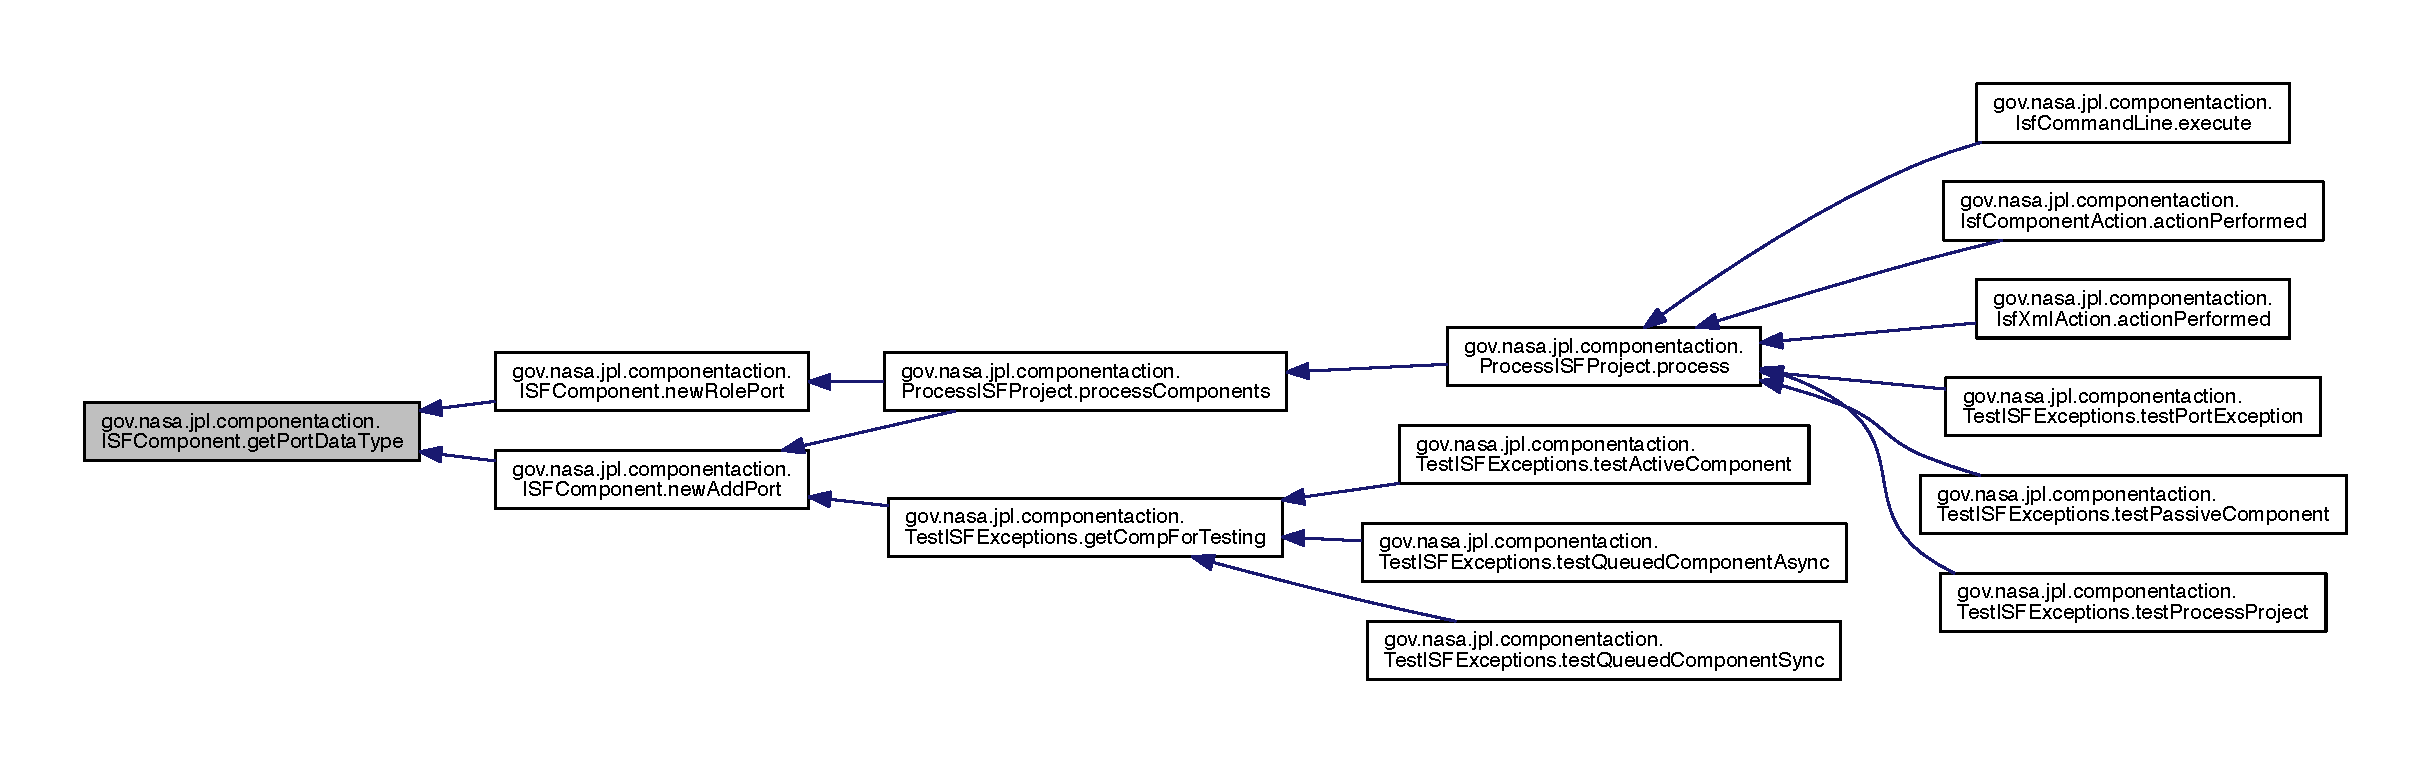
\includegraphics[width=350pt]{classgov_1_1nasa_1_1jpl_1_1componentaction_1_1_i_s_f_component_a18d1885312f59b16ed2a43ca059d050c_icgraph}
\end{center}
\end{figure}


\index{gov\+::nasa\+::jpl\+::componentaction\+::\+I\+S\+F\+Component@{gov\+::nasa\+::jpl\+::componentaction\+::\+I\+S\+F\+Component}!get\+Port\+Data\+Type\+Namespace@{get\+Port\+Data\+Type\+Namespace}}
\index{get\+Port\+Data\+Type\+Namespace@{get\+Port\+Data\+Type\+Namespace}!gov\+::nasa\+::jpl\+::componentaction\+::\+I\+S\+F\+Component@{gov\+::nasa\+::jpl\+::componentaction\+::\+I\+S\+F\+Component}}
\subsubsection[{get\+Port\+Data\+Type\+Namespace(\+Element port\+Element)}]{\setlength{\rightskip}{0pt plus 5cm}String gov.\+nasa.\+jpl.\+componentaction.\+I\+S\+F\+Component.\+get\+Port\+Data\+Type\+Namespace (
\begin{DoxyParamCaption}
\item[{Element}]{port\+Element}
\end{DoxyParamCaption}
)}\label{classgov_1_1nasa_1_1jpl_1_1componentaction_1_1_i_s_f_component_ab070273e1864833d0b55062dc224ae33}
This returns the port data type without the full path. It also tags on the Namespace.


\begin{DoxyParams}{Parameters}
{\em port\+Element} & \\
\hline
\end{DoxyParams}
\begin{DoxyReturn}{Returns}
data type + \textquotesingle{}\+:\+:\textquotesingle{} + name space 
\end{DoxyReturn}


Here is the call graph for this function\+:
\nopagebreak
\begin{figure}[H]
\begin{center}
\leavevmode
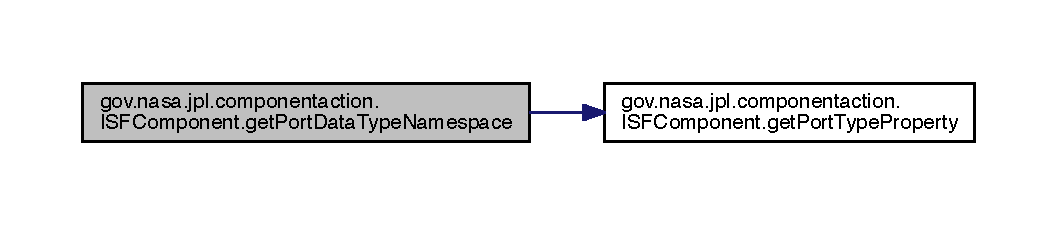
\includegraphics[width=350pt]{classgov_1_1nasa_1_1jpl_1_1componentaction_1_1_i_s_f_component_ab070273e1864833d0b55062dc224ae33_cgraph}
\end{center}
\end{figure}




Here is the caller graph for this function\+:
\nopagebreak
\begin{figure}[H]
\begin{center}
\leavevmode
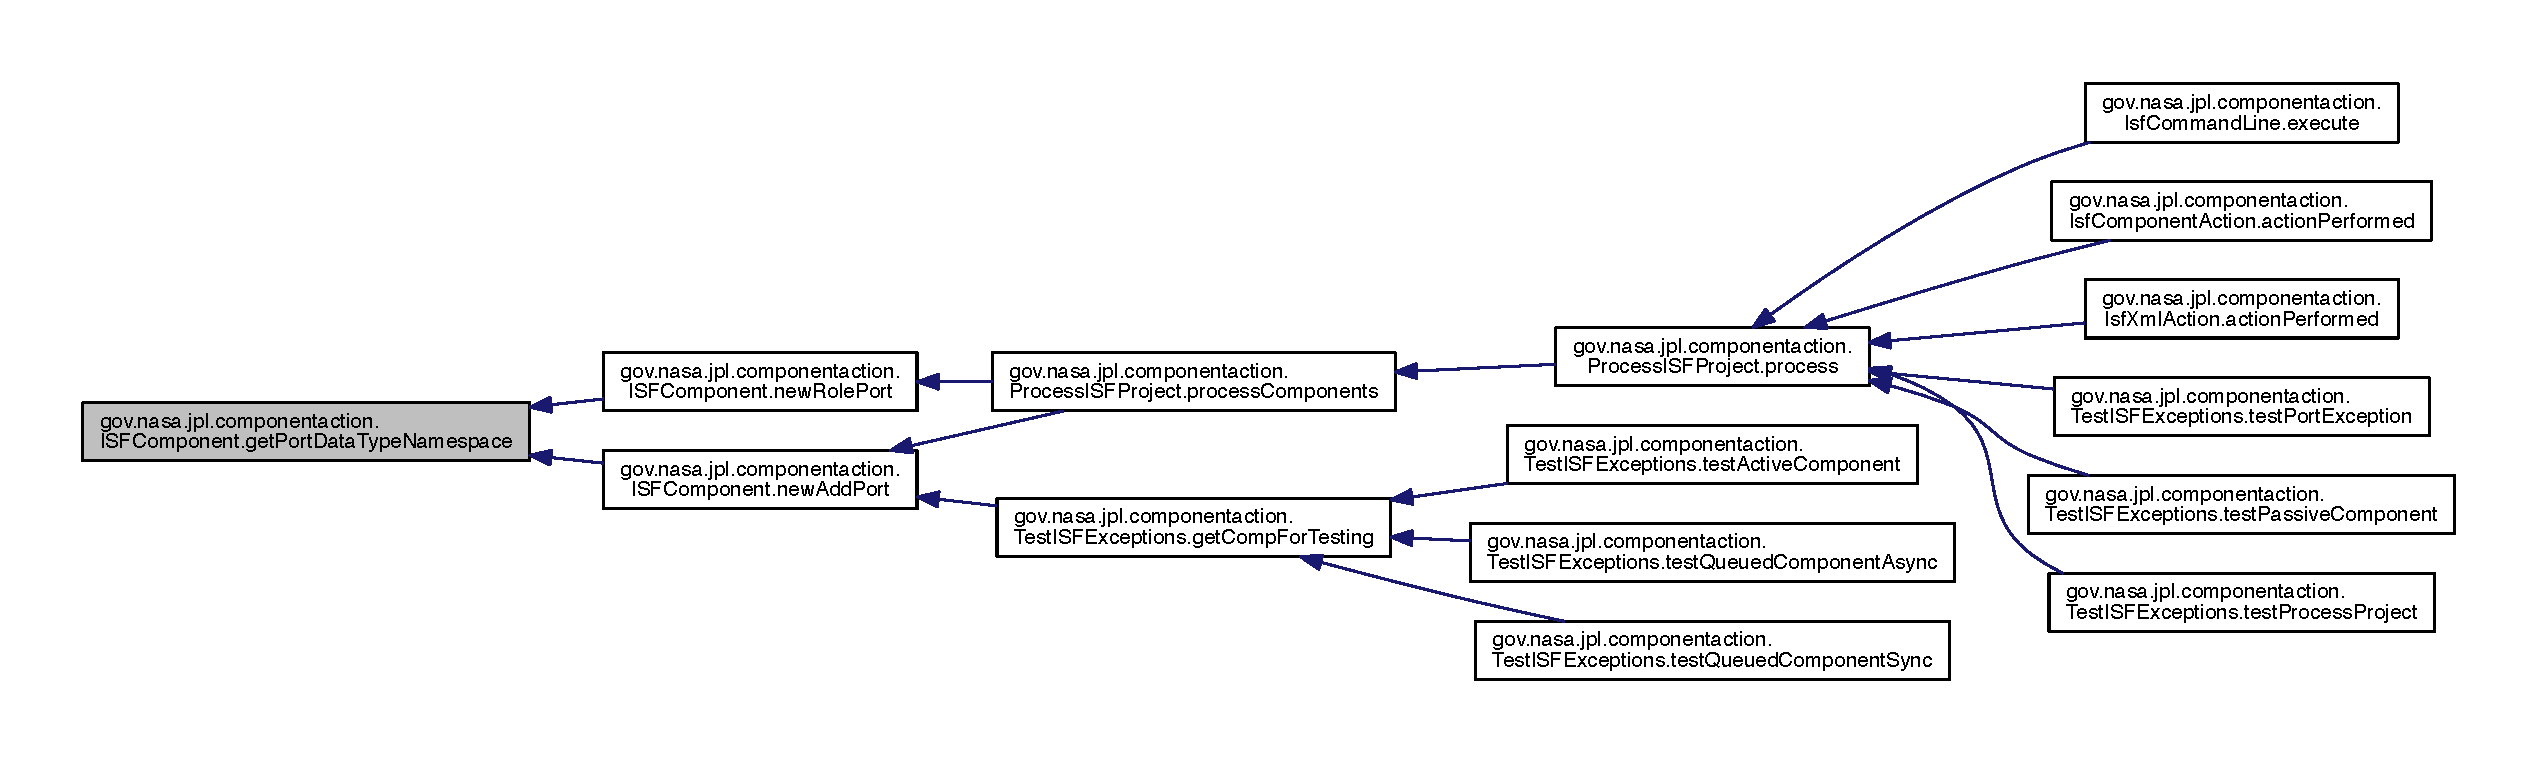
\includegraphics[width=350pt]{classgov_1_1nasa_1_1jpl_1_1componentaction_1_1_i_s_f_component_ab070273e1864833d0b55062dc224ae33_icgraph}
\end{center}
\end{figure}


\index{gov\+::nasa\+::jpl\+::componentaction\+::\+I\+S\+F\+Component@{gov\+::nasa\+::jpl\+::componentaction\+::\+I\+S\+F\+Component}!get\+Port\+Hash\+List@{get\+Port\+Hash\+List}}
\index{get\+Port\+Hash\+List@{get\+Port\+Hash\+List}!gov\+::nasa\+::jpl\+::componentaction\+::\+I\+S\+F\+Component@{gov\+::nasa\+::jpl\+::componentaction\+::\+I\+S\+F\+Component}}
\subsubsection[{get\+Port\+Hash\+List()}]{\setlength{\rightskip}{0pt plus 5cm}Hash\+Map$<$String, {\bf port\+Object}$>$ gov.\+nasa.\+jpl.\+componentaction.\+I\+S\+F\+Component.\+get\+Port\+Hash\+List (
\begin{DoxyParamCaption}
{}
\end{DoxyParamCaption}
)}\label{classgov_1_1nasa_1_1jpl_1_1componentaction_1_1_i_s_f_component_ac676b50d41701ce8bbccb7687181c679}
Returns the filt\+List Hash\+Map, a map with a string associated with a port object. \begin{DoxyReturn}{Returns}
Hash\+Map 
\end{DoxyReturn}
\index{gov\+::nasa\+::jpl\+::componentaction\+::\+I\+S\+F\+Component@{gov\+::nasa\+::jpl\+::componentaction\+::\+I\+S\+F\+Component}!get\+Port\+Name@{get\+Port\+Name}}
\index{get\+Port\+Name@{get\+Port\+Name}!gov\+::nasa\+::jpl\+::componentaction\+::\+I\+S\+F\+Component@{gov\+::nasa\+::jpl\+::componentaction\+::\+I\+S\+F\+Component}}
\subsubsection[{get\+Port\+Name(\+Element port\+Element)}]{\setlength{\rightskip}{0pt plus 5cm}String gov.\+nasa.\+jpl.\+componentaction.\+I\+S\+F\+Component.\+get\+Port\+Name (
\begin{DoxyParamCaption}
\item[{Element}]{port\+Element}
\end{DoxyParamCaption}
)}\label{classgov_1_1nasa_1_1jpl_1_1componentaction_1_1_i_s_f_component_a38a82f9a572463e0740ddbf3a1bfddf5}
Returns the port name.


\begin{DoxyParams}{Parameters}
{\em port\+Element} & port which the name will be extracted from \\
\hline
\end{DoxyParams}
\begin{DoxyReturn}{Returns}
The name of the port 
\end{DoxyReturn}
\index{gov\+::nasa\+::jpl\+::componentaction\+::\+I\+S\+F\+Component@{gov\+::nasa\+::jpl\+::componentaction\+::\+I\+S\+F\+Component}!get\+Port\+Property@{get\+Port\+Property}}
\index{get\+Port\+Property@{get\+Port\+Property}!gov\+::nasa\+::jpl\+::componentaction\+::\+I\+S\+F\+Component@{gov\+::nasa\+::jpl\+::componentaction\+::\+I\+S\+F\+Component}}
\subsubsection[{get\+Port\+Property(\+Element port\+Element, String property)}]{\setlength{\rightskip}{0pt plus 5cm}String gov.\+nasa.\+jpl.\+componentaction.\+I\+S\+F\+Component.\+get\+Port\+Property (
\begin{DoxyParamCaption}
\item[{Element}]{port\+Element, }
\item[{String}]{property}
\end{DoxyParamCaption}
)}\label{classgov_1_1nasa_1_1jpl_1_1componentaction_1_1_i_s_f_component_a9f264ef3ba76a1ecc5aa42e13cd93221}
Returns the property value of async\+\_\+input stereotype of the input element argument. 
\begin{DoxyParams}{Parameters}
{\em port\+Element} & Element of the port type \\
\hline
{\em property} & String of value to be looked for in the stereotype async\+\_\+input \\
\hline
\end{DoxyParams}
\begin{DoxyReturn}{Returns}
The value of the attribute from property 
\end{DoxyReturn}


Here is the caller graph for this function\+:
\nopagebreak
\begin{figure}[H]
\begin{center}
\leavevmode
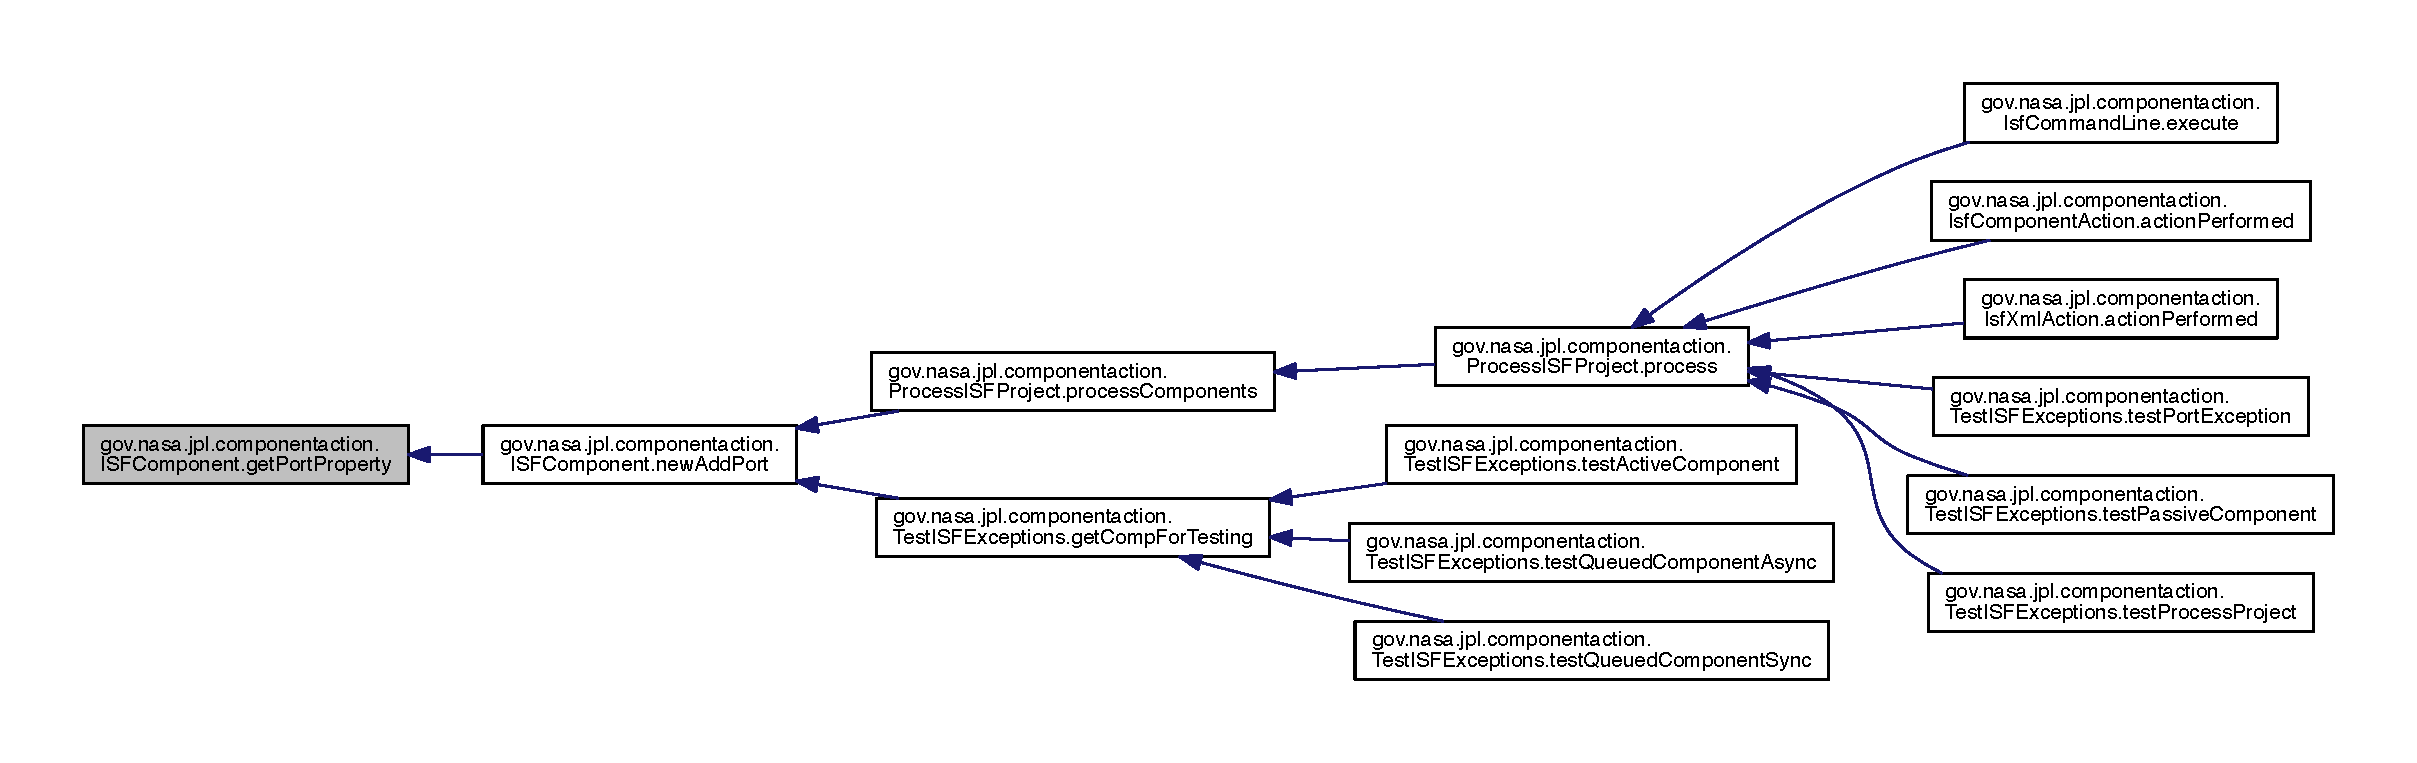
\includegraphics[width=350pt]{classgov_1_1nasa_1_1jpl_1_1componentaction_1_1_i_s_f_component_a9f264ef3ba76a1ecc5aa42e13cd93221_icgraph}
\end{center}
\end{figure}


\index{gov\+::nasa\+::jpl\+::componentaction\+::\+I\+S\+F\+Component@{gov\+::nasa\+::jpl\+::componentaction\+::\+I\+S\+F\+Component}!get\+Port\+Stereotype@{get\+Port\+Stereotype}}
\index{get\+Port\+Stereotype@{get\+Port\+Stereotype}!gov\+::nasa\+::jpl\+::componentaction\+::\+I\+S\+F\+Component@{gov\+::nasa\+::jpl\+::componentaction\+::\+I\+S\+F\+Component}}
\subsubsection[{get\+Port\+Stereotype(\+Element port\+Element)}]{\setlength{\rightskip}{0pt plus 5cm}String gov.\+nasa.\+jpl.\+componentaction.\+I\+S\+F\+Component.\+get\+Port\+Stereotype (
\begin{DoxyParamCaption}
\item[{Element}]{port\+Element}
\end{DoxyParamCaption}
)}\label{classgov_1_1nasa_1_1jpl_1_1componentaction_1_1_i_s_f_component_a27979d4dedfc260f3e44655824cf3d3e}
Returns the port stereotype.


\begin{DoxyParams}{Parameters}
{\em port\+Element} & port which the stereotype will be extracted from \\
\hline
\end{DoxyParams}
\begin{DoxyReturn}{Returns}
The stereotype of the port 
\end{DoxyReturn}


Here is the caller graph for this function\+:
\nopagebreak
\begin{figure}[H]
\begin{center}
\leavevmode
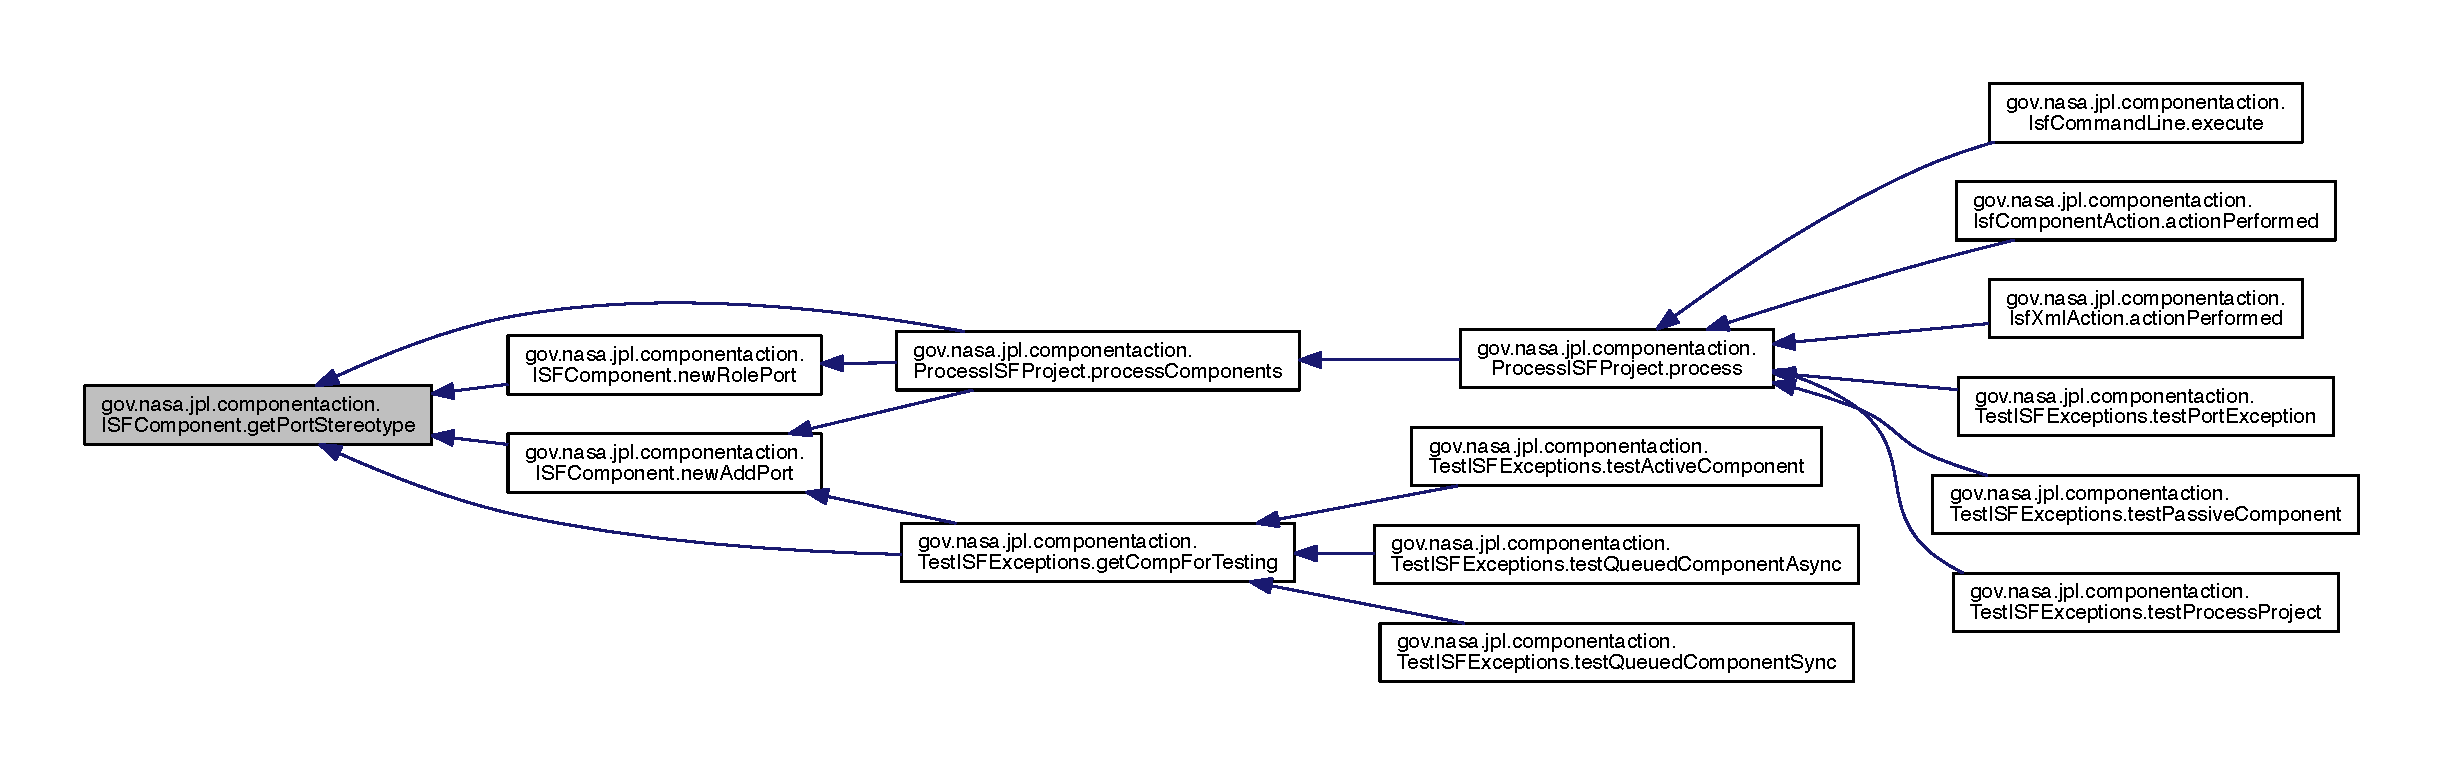
\includegraphics[width=350pt]{classgov_1_1nasa_1_1jpl_1_1componentaction_1_1_i_s_f_component_a27979d4dedfc260f3e44655824cf3d3e_icgraph}
\end{center}
\end{figure}


\index{gov\+::nasa\+::jpl\+::componentaction\+::\+I\+S\+F\+Component@{gov\+::nasa\+::jpl\+::componentaction\+::\+I\+S\+F\+Component}!get\+Port\+Type\+Property@{get\+Port\+Type\+Property}}
\index{get\+Port\+Type\+Property@{get\+Port\+Type\+Property}!gov\+::nasa\+::jpl\+::componentaction\+::\+I\+S\+F\+Component@{gov\+::nasa\+::jpl\+::componentaction\+::\+I\+S\+F\+Component}}
\subsubsection[{get\+Port\+Type\+Property(\+Element port\+Element, String property)}]{\setlength{\rightskip}{0pt plus 5cm}String gov.\+nasa.\+jpl.\+componentaction.\+I\+S\+F\+Component.\+get\+Port\+Type\+Property (
\begin{DoxyParamCaption}
\item[{Element}]{port\+Element, }
\item[{String}]{property}
\end{DoxyParamCaption}
)}\label{classgov_1_1nasa_1_1jpl_1_1componentaction_1_1_i_s_f_component_a92968a00a3cfed968283fddf0fd46204}
Returns the property value of Port\+Type stereotype of the input element argument. 
\begin{DoxyParams}{Parameters}
{\em port\+Element} & Element of the port type \\
\hline
{\em property} & String of value to be looked for in the stereotype Port\+Type \\
\hline
\end{DoxyParams}
\begin{DoxyReturn}{Returns}
The value of the attribute from property 
\end{DoxyReturn}


Here is the caller graph for this function\+:
\nopagebreak
\begin{figure}[H]
\begin{center}
\leavevmode
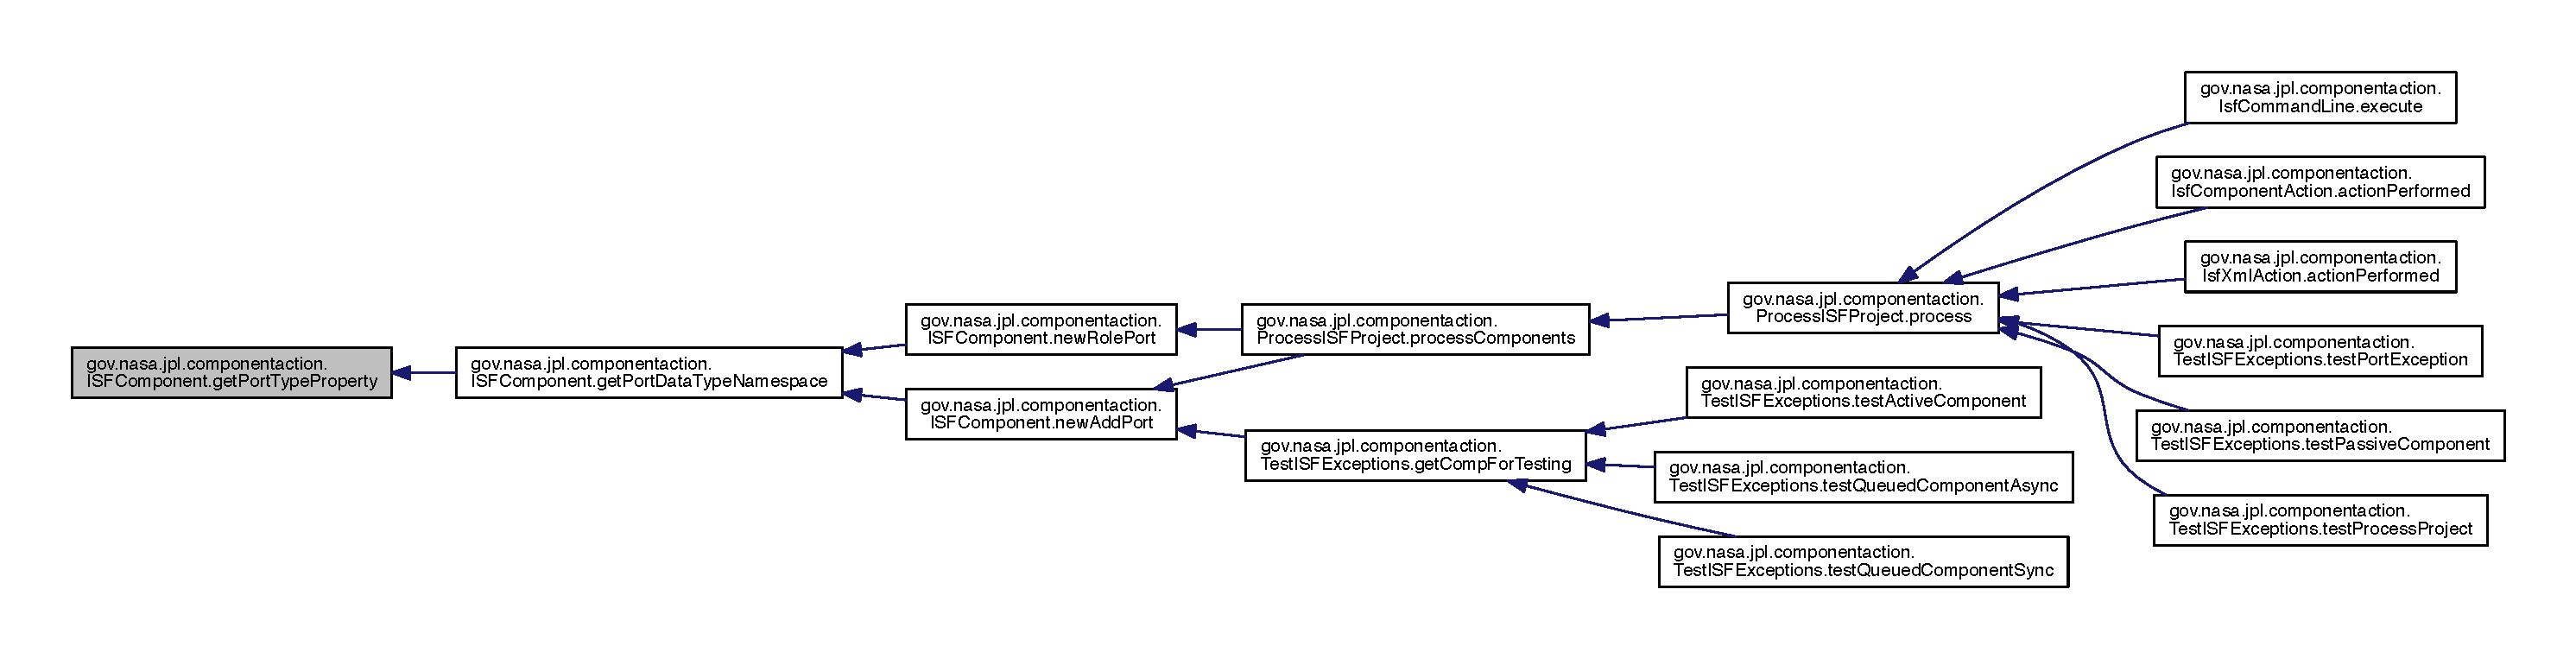
\includegraphics[width=350pt]{classgov_1_1nasa_1_1jpl_1_1componentaction_1_1_i_s_f_component_a92968a00a3cfed968283fddf0fd46204_icgraph}
\end{center}
\end{figure}


\index{gov\+::nasa\+::jpl\+::componentaction\+::\+I\+S\+F\+Component@{gov\+::nasa\+::jpl\+::componentaction\+::\+I\+S\+F\+Component}!get\+Stereotype@{get\+Stereotype}}
\index{get\+Stereotype@{get\+Stereotype}!gov\+::nasa\+::jpl\+::componentaction\+::\+I\+S\+F\+Component@{gov\+::nasa\+::jpl\+::componentaction\+::\+I\+S\+F\+Component}}
\subsubsection[{get\+Stereotype()}]{\setlength{\rightskip}{0pt plus 5cm}String gov.\+nasa.\+jpl.\+componentaction.\+I\+S\+F\+Component.\+get\+Stereotype (
\begin{DoxyParamCaption}
{}
\end{DoxyParamCaption}
)}\label{classgov_1_1nasa_1_1jpl_1_1componentaction_1_1_i_s_f_component_a555d144d31719e3845cba79b9cab02c1}
Returns comp\+Stereotype \begin{DoxyReturn}{Returns}
the stereotype of the object 
\end{DoxyReturn}
\index{gov\+::nasa\+::jpl\+::componentaction\+::\+I\+S\+F\+Component@{gov\+::nasa\+::jpl\+::componentaction\+::\+I\+S\+F\+Component}!get\+U\+RI@{get\+U\+RI}}
\index{get\+U\+RI@{get\+U\+RI}!gov\+::nasa\+::jpl\+::componentaction\+::\+I\+S\+F\+Component@{gov\+::nasa\+::jpl\+::componentaction\+::\+I\+S\+F\+Component}}
\subsubsection[{get\+U\+R\+I()}]{\setlength{\rightskip}{0pt plus 5cm}String gov.\+nasa.\+jpl.\+componentaction.\+I\+S\+F\+Component.\+get\+U\+RI (
\begin{DoxyParamCaption}
{}
\end{DoxyParamCaption}
)}\label{classgov_1_1nasa_1_1jpl_1_1componentaction_1_1_i_s_f_component_aa584ab5490b187caa1681a8f2f64de3f}
Returns the component\textquotesingle{}s U\+RI, which is the location in the tree hierarchy. \begin{DoxyReturn}{Returns}
string of position in hierarchy 
\end{DoxyReturn}
\index{gov\+::nasa\+::jpl\+::componentaction\+::\+I\+S\+F\+Component@{gov\+::nasa\+::jpl\+::componentaction\+::\+I\+S\+F\+Component}!is\+Valid@{is\+Valid}}
\index{is\+Valid@{is\+Valid}!gov\+::nasa\+::jpl\+::componentaction\+::\+I\+S\+F\+Component@{gov\+::nasa\+::jpl\+::componentaction\+::\+I\+S\+F\+Component}}
\subsubsection[{is\+Valid(\+String stereotype, String port\+Type, boolean at\+Least\+One)}]{\setlength{\rightskip}{0pt plus 5cm}boolean gov.\+nasa.\+jpl.\+componentaction.\+I\+S\+F\+Component.\+is\+Valid (
\begin{DoxyParamCaption}
\item[{String}]{stereotype, }
\item[{String}]{port\+Type, }
\item[{boolean}]{at\+Least\+One}
\end{DoxyParamCaption}
)}\label{classgov_1_1nasa_1_1jpl_1_1componentaction_1_1_i_s_f_component_a73ef1f98a84fdbb1e835fcdecbccb18c}
Checks if a component is of a specific stereotype If so, checks if the component satisfies the requirement for a specific port type 
\begin{DoxyParams}{Parameters}
{\em stereotype} & the stereotype the component should have \\
\hline
{\em port\+Type} & the port type to check for \\
\hline
{\em at\+Least\+One} & if the component should have the port type \\
\hline
\end{DoxyParams}


Here is the caller graph for this function\+:
\nopagebreak
\begin{figure}[H]
\begin{center}
\leavevmode
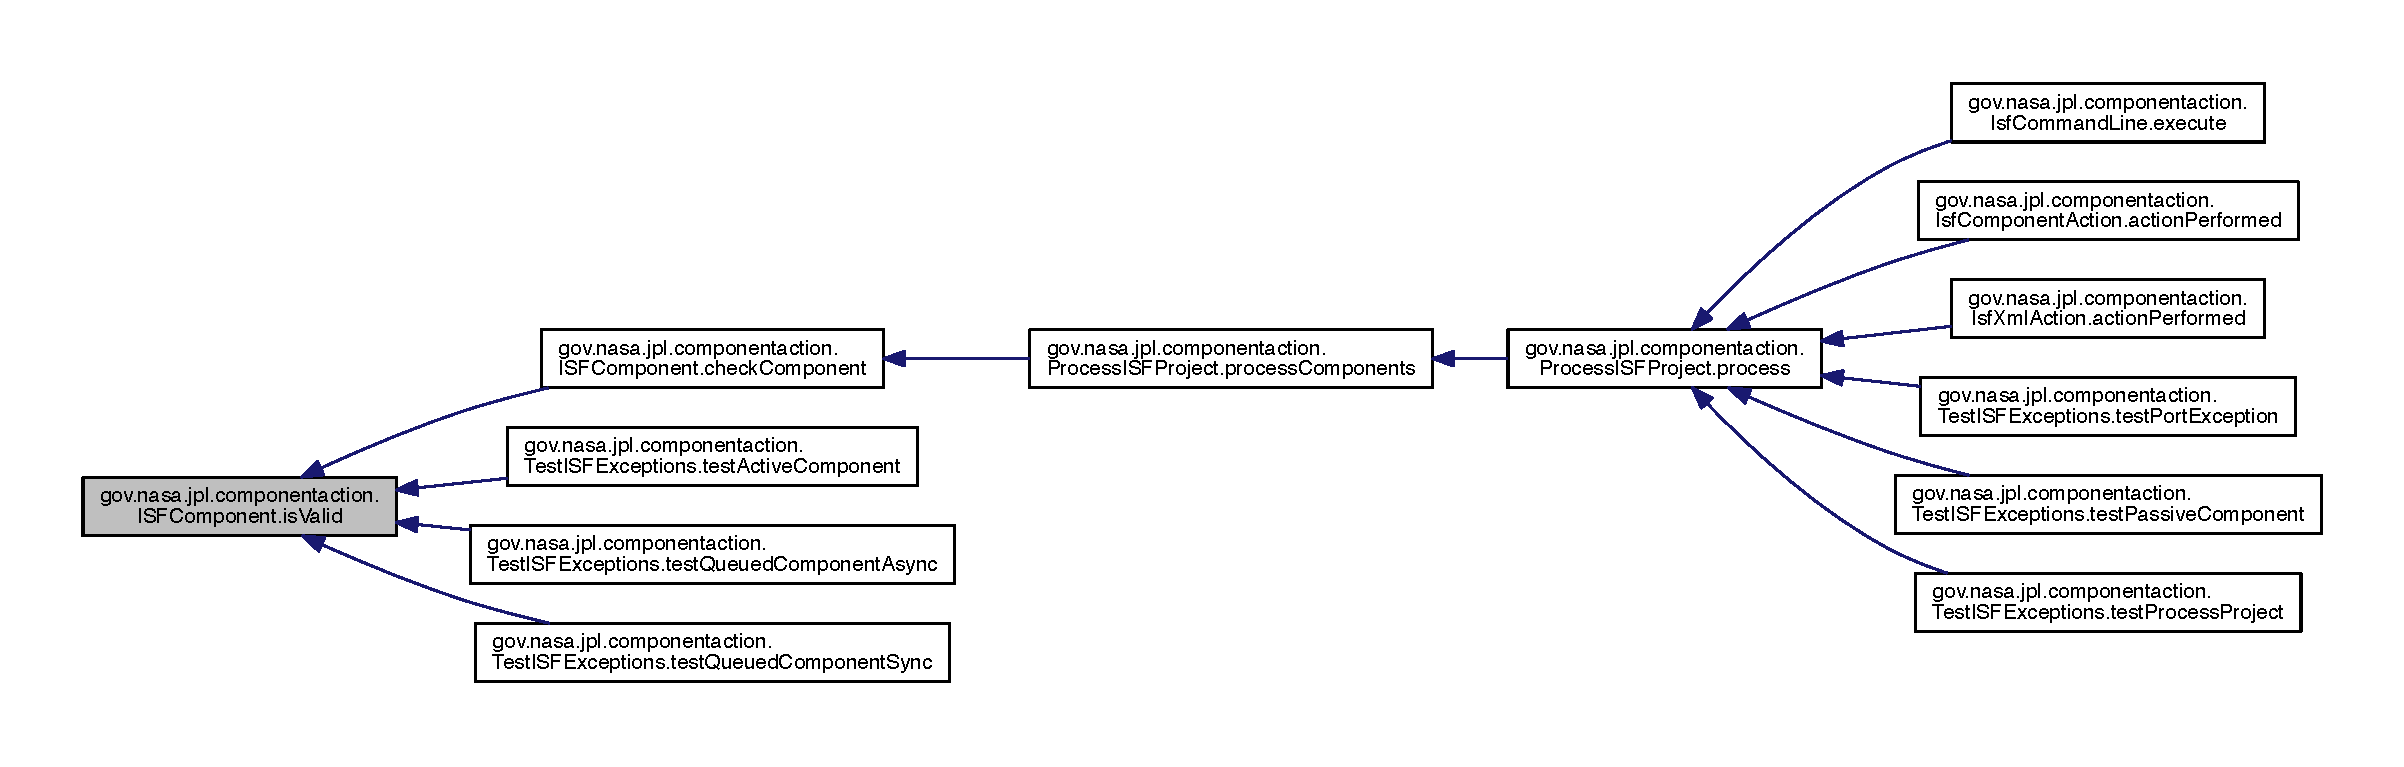
\includegraphics[width=350pt]{classgov_1_1nasa_1_1jpl_1_1componentaction_1_1_i_s_f_component_a73ef1f98a84fdbb1e835fcdecbccb18c_icgraph}
\end{center}
\end{figure}


\index{gov\+::nasa\+::jpl\+::componentaction\+::\+I\+S\+F\+Component@{gov\+::nasa\+::jpl\+::componentaction\+::\+I\+S\+F\+Component}!new\+Add\+Port@{new\+Add\+Port}}
\index{new\+Add\+Port@{new\+Add\+Port}!gov\+::nasa\+::jpl\+::componentaction\+::\+I\+S\+F\+Component@{gov\+::nasa\+::jpl\+::componentaction\+::\+I\+S\+F\+Component}}
\subsubsection[{new\+Add\+Port(\+Element port\+Element)}]{\setlength{\rightskip}{0pt plus 5cm}void gov.\+nasa.\+jpl.\+componentaction.\+I\+S\+F\+Component.\+new\+Add\+Port (
\begin{DoxyParamCaption}
\item[{Element}]{port\+Element}
\end{DoxyParamCaption}
) throws {\bf Port\+Exception}}\label{classgov_1_1nasa_1_1jpl_1_1componentaction_1_1_i_s_f_component_a092093642fbaab5c3cf710bef9af6e62}
Creates a new port object using the port Element inputed. This processes the port and can throw an exception if something in the port is illegal. It also adds the port into fill\+List.


\begin{DoxyParams}{Parameters}
{\em port\+Element} & \\
\hline
\end{DoxyParams}

\begin{DoxyExceptions}{Exceptions}
{\em \doxyref{Port\+Exception}{p.}{classgov_1_1nasa_1_1jpl_1_1componentaction_1_1_port_exception}} & \\
\hline
\end{DoxyExceptions}


Here is the call graph for this function\+:
\nopagebreak
\begin{figure}[H]
\begin{center}
\leavevmode
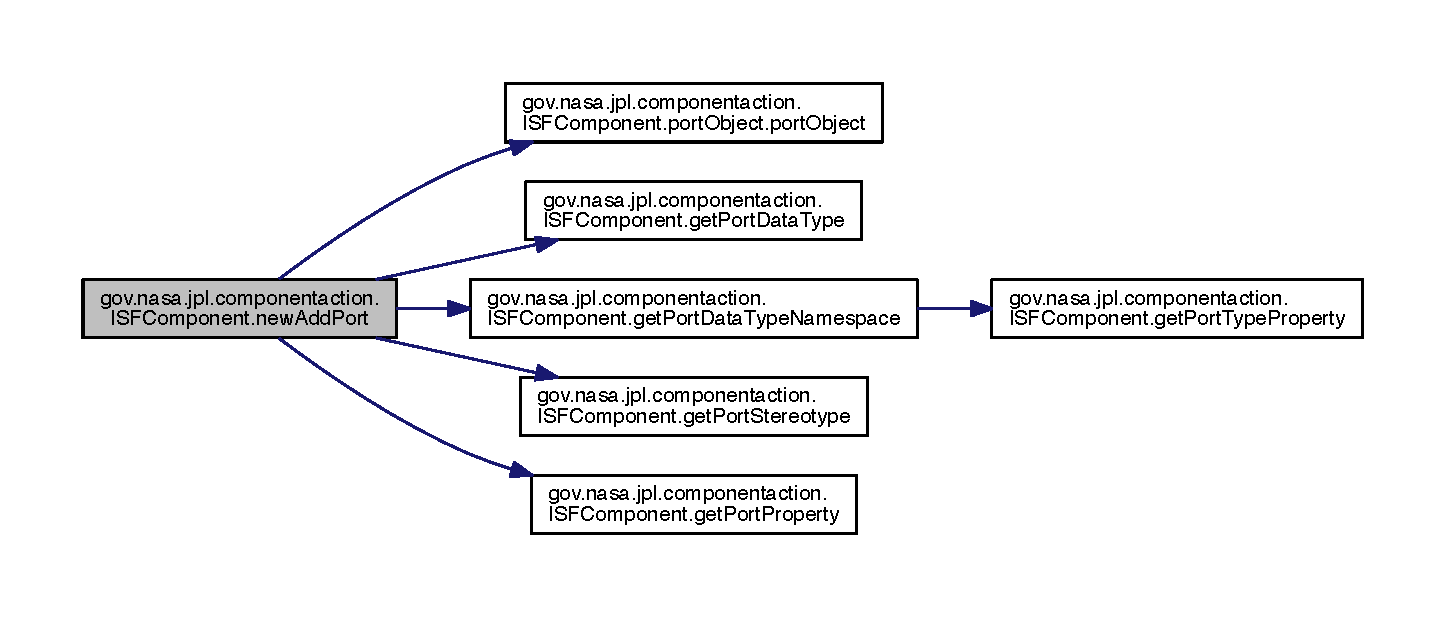
\includegraphics[width=350pt]{classgov_1_1nasa_1_1jpl_1_1componentaction_1_1_i_s_f_component_a092093642fbaab5c3cf710bef9af6e62_cgraph}
\end{center}
\end{figure}




Here is the caller graph for this function\+:
\nopagebreak
\begin{figure}[H]
\begin{center}
\leavevmode
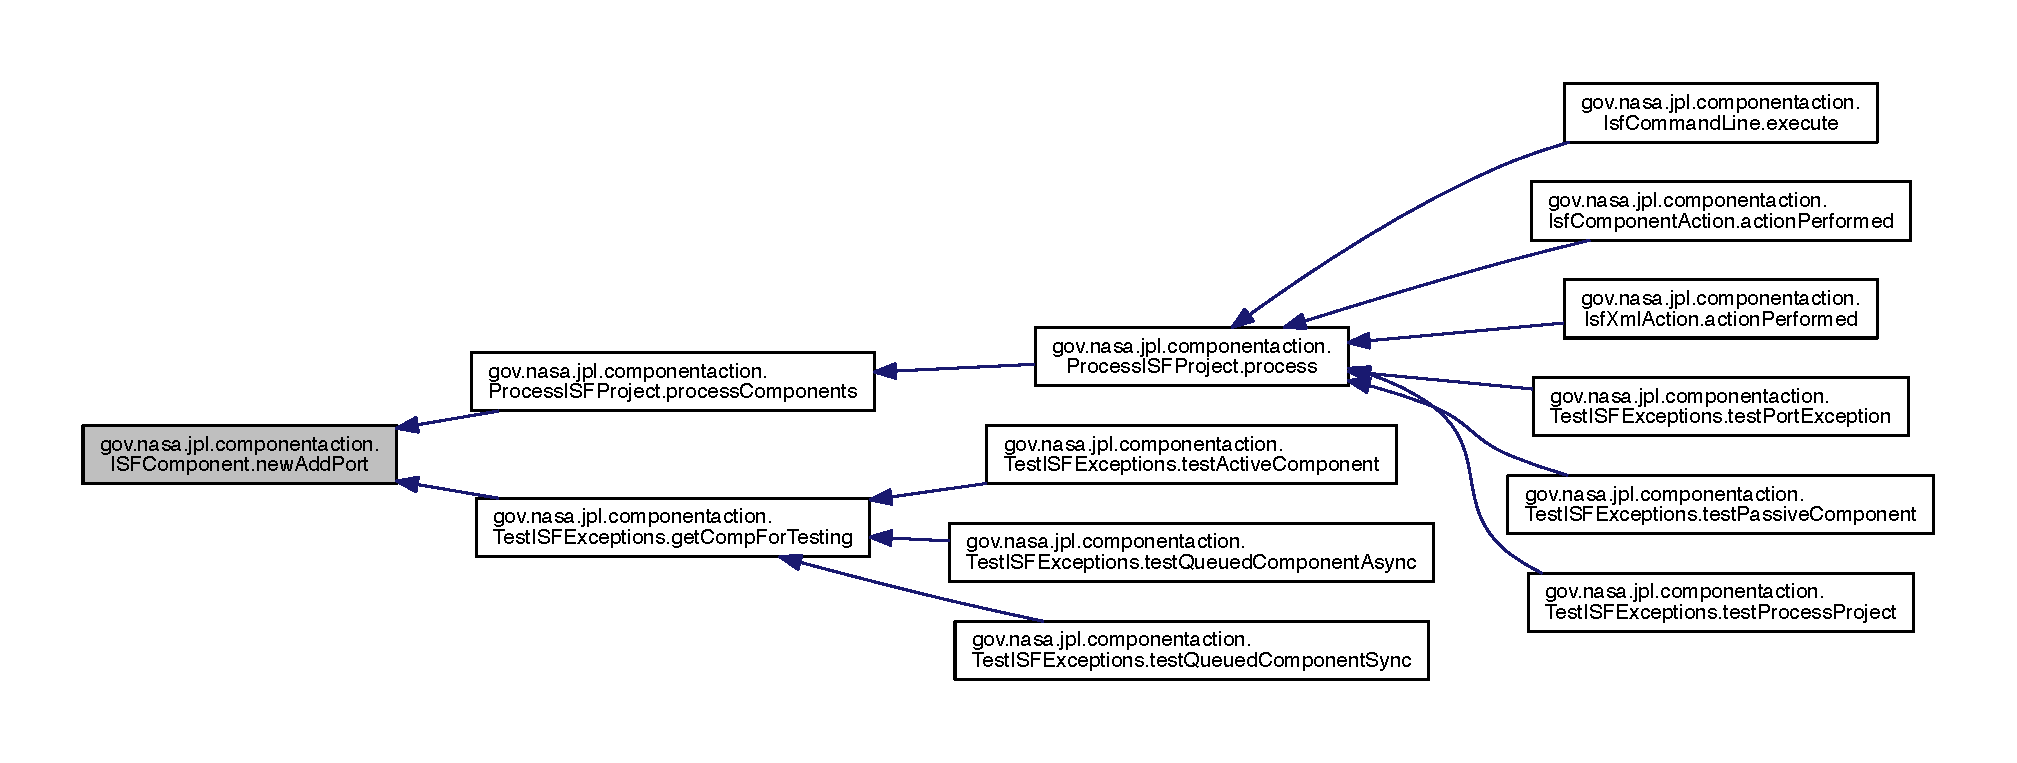
\includegraphics[width=350pt]{classgov_1_1nasa_1_1jpl_1_1componentaction_1_1_i_s_f_component_a092093642fbaab5c3cf710bef9af6e62_icgraph}
\end{center}
\end{figure}


\index{gov\+::nasa\+::jpl\+::componentaction\+::\+I\+S\+F\+Component@{gov\+::nasa\+::jpl\+::componentaction\+::\+I\+S\+F\+Component}!new\+Role\+Port@{new\+Role\+Port}}
\index{new\+Role\+Port@{new\+Role\+Port}!gov\+::nasa\+::jpl\+::componentaction\+::\+I\+S\+F\+Component@{gov\+::nasa\+::jpl\+::componentaction\+::\+I\+S\+F\+Component}}
\subsubsection[{new\+Role\+Port(\+Element port\+Element)}]{\setlength{\rightskip}{0pt plus 5cm}void gov.\+nasa.\+jpl.\+componentaction.\+I\+S\+F\+Component.\+new\+Role\+Port (
\begin{DoxyParamCaption}
\item[{Element}]{port\+Element}
\end{DoxyParamCaption}
) throws {\bf Port\+Exception}}\label{classgov_1_1nasa_1_1jpl_1_1componentaction_1_1_i_s_f_component_a9c0cb98c724eb5022707663242c3460b}
Creates a new port object using the port Element inputed. This processes the port and can throw an exception if something in the port is illegal. It also adds the port into fill\+List.


\begin{DoxyParams}{Parameters}
{\em port\+Element} & \\
\hline
\end{DoxyParams}

\begin{DoxyExceptions}{Exceptions}
{\em \doxyref{Port\+Exception}{p.}{classgov_1_1nasa_1_1jpl_1_1componentaction_1_1_port_exception}} & \\
\hline
\end{DoxyExceptions}


Here is the call graph for this function\+:
\nopagebreak
\begin{figure}[H]
\begin{center}
\leavevmode
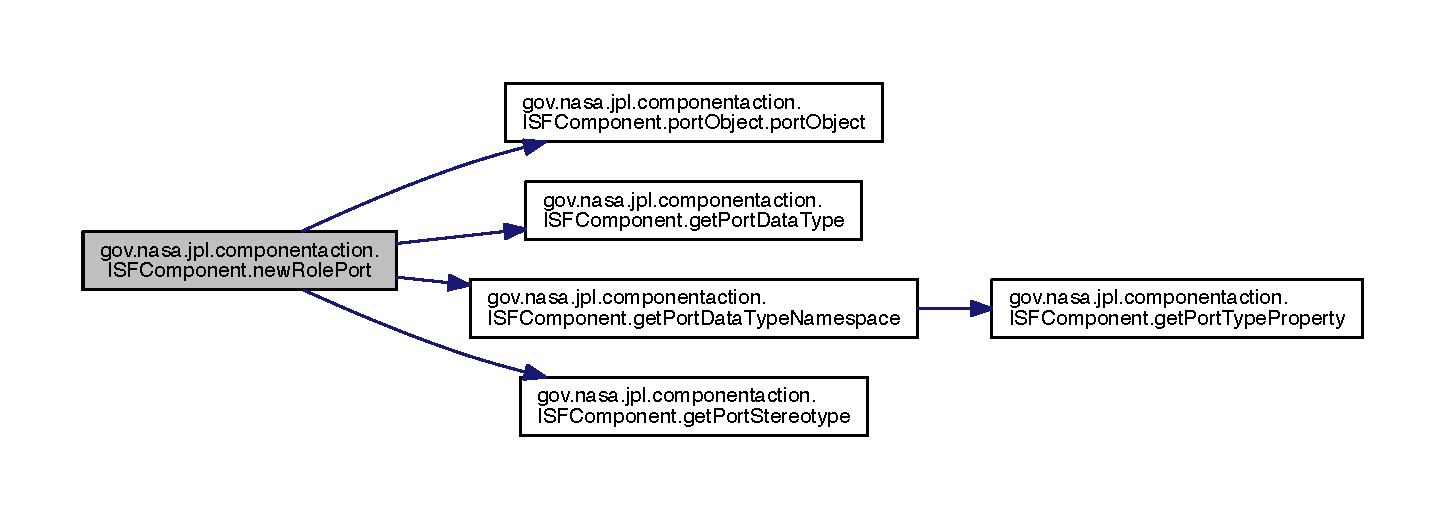
\includegraphics[width=350pt]{classgov_1_1nasa_1_1jpl_1_1componentaction_1_1_i_s_f_component_a9c0cb98c724eb5022707663242c3460b_cgraph}
\end{center}
\end{figure}




Here is the caller graph for this function\+:
\nopagebreak
\begin{figure}[H]
\begin{center}
\leavevmode
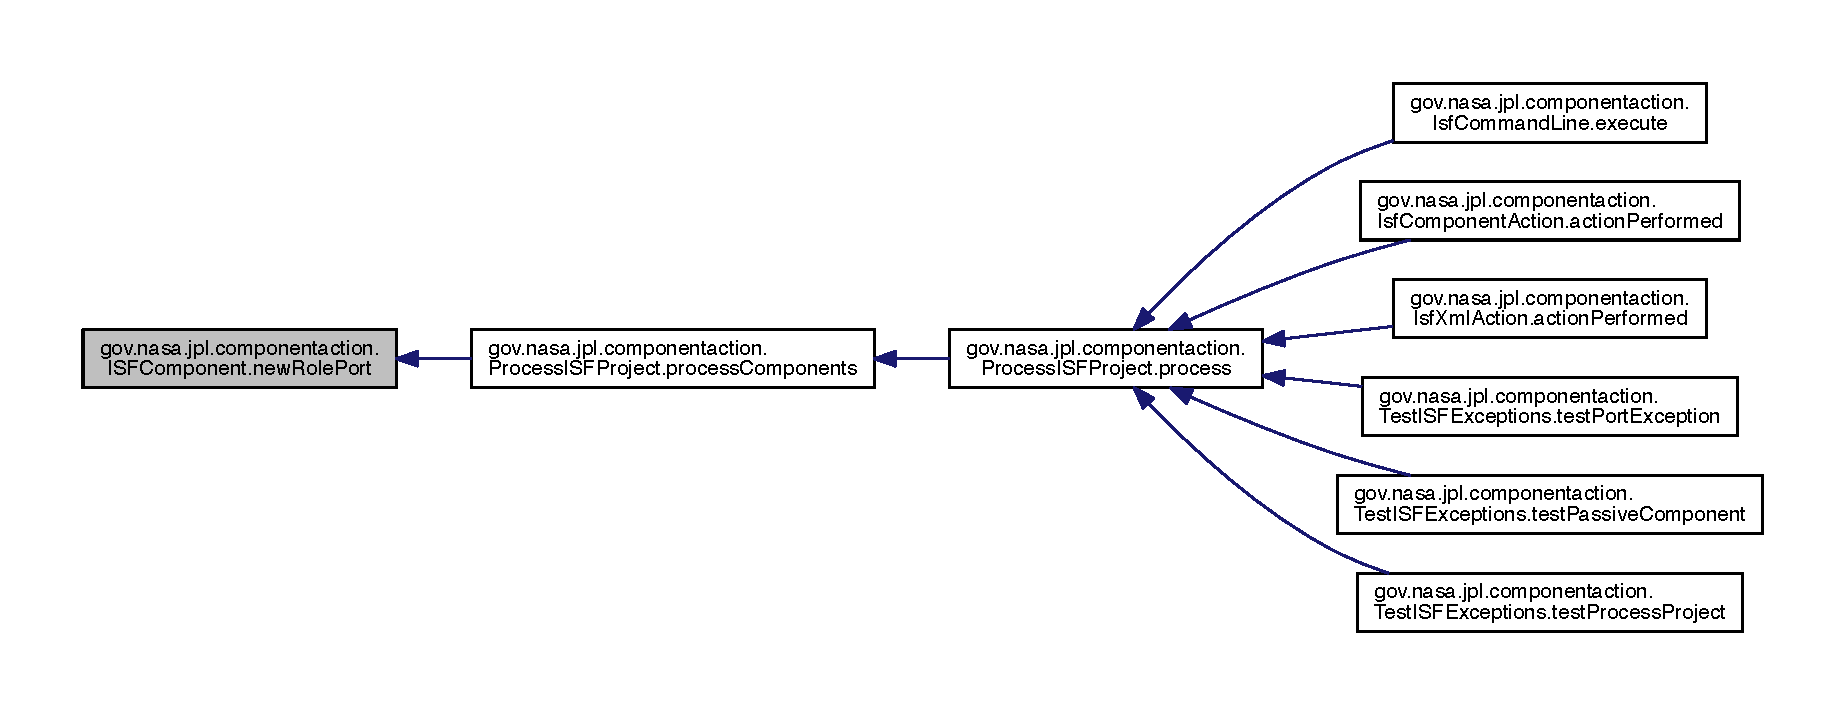
\includegraphics[width=350pt]{classgov_1_1nasa_1_1jpl_1_1componentaction_1_1_i_s_f_component_a9c0cb98c724eb5022707663242c3460b_icgraph}
\end{center}
\end{figure}


\index{gov\+::nasa\+::jpl\+::componentaction\+::\+I\+S\+F\+Component@{gov\+::nasa\+::jpl\+::componentaction\+::\+I\+S\+F\+Component}!print@{print}}
\index{print@{print}!gov\+::nasa\+::jpl\+::componentaction\+::\+I\+S\+F\+Component@{gov\+::nasa\+::jpl\+::componentaction\+::\+I\+S\+F\+Component}}
\subsubsection[{print()}]{\setlength{\rightskip}{0pt plus 5cm}void gov.\+nasa.\+jpl.\+componentaction.\+I\+S\+F\+Component.\+print (
\begin{DoxyParamCaption}
{}
\end{DoxyParamCaption}
)}\label{classgov_1_1nasa_1_1jpl_1_1componentaction_1_1_i_s_f_component_a4c883e8f6a61392e5ef253c38689ba73}
\index{gov\+::nasa\+::jpl\+::componentaction\+::\+I\+S\+F\+Component@{gov\+::nasa\+::jpl\+::componentaction\+::\+I\+S\+F\+Component}!set\+Stereo\+Type@{set\+Stereo\+Type}}
\index{set\+Stereo\+Type@{set\+Stereo\+Type}!gov\+::nasa\+::jpl\+::componentaction\+::\+I\+S\+F\+Component@{gov\+::nasa\+::jpl\+::componentaction\+::\+I\+S\+F\+Component}}
\subsubsection[{set\+Stereo\+Type(\+String comp\+Stereotype)}]{\setlength{\rightskip}{0pt plus 5cm}void gov.\+nasa.\+jpl.\+componentaction.\+I\+S\+F\+Component.\+set\+Stereo\+Type (
\begin{DoxyParamCaption}
\item[{String}]{comp\+Stereotype}
\end{DoxyParamCaption}
)}\label{classgov_1_1nasa_1_1jpl_1_1componentaction_1_1_i_s_f_component_ac9317d03a2dcd968d3fa39f5a92bd350}
Sets the component stereotype string value 
\begin{DoxyParams}{Parameters}
{\em comp\+Stereotype} & Stereotype string \\
\hline
\end{DoxyParams}


Here is the caller graph for this function\+:
\nopagebreak
\begin{figure}[H]
\begin{center}
\leavevmode
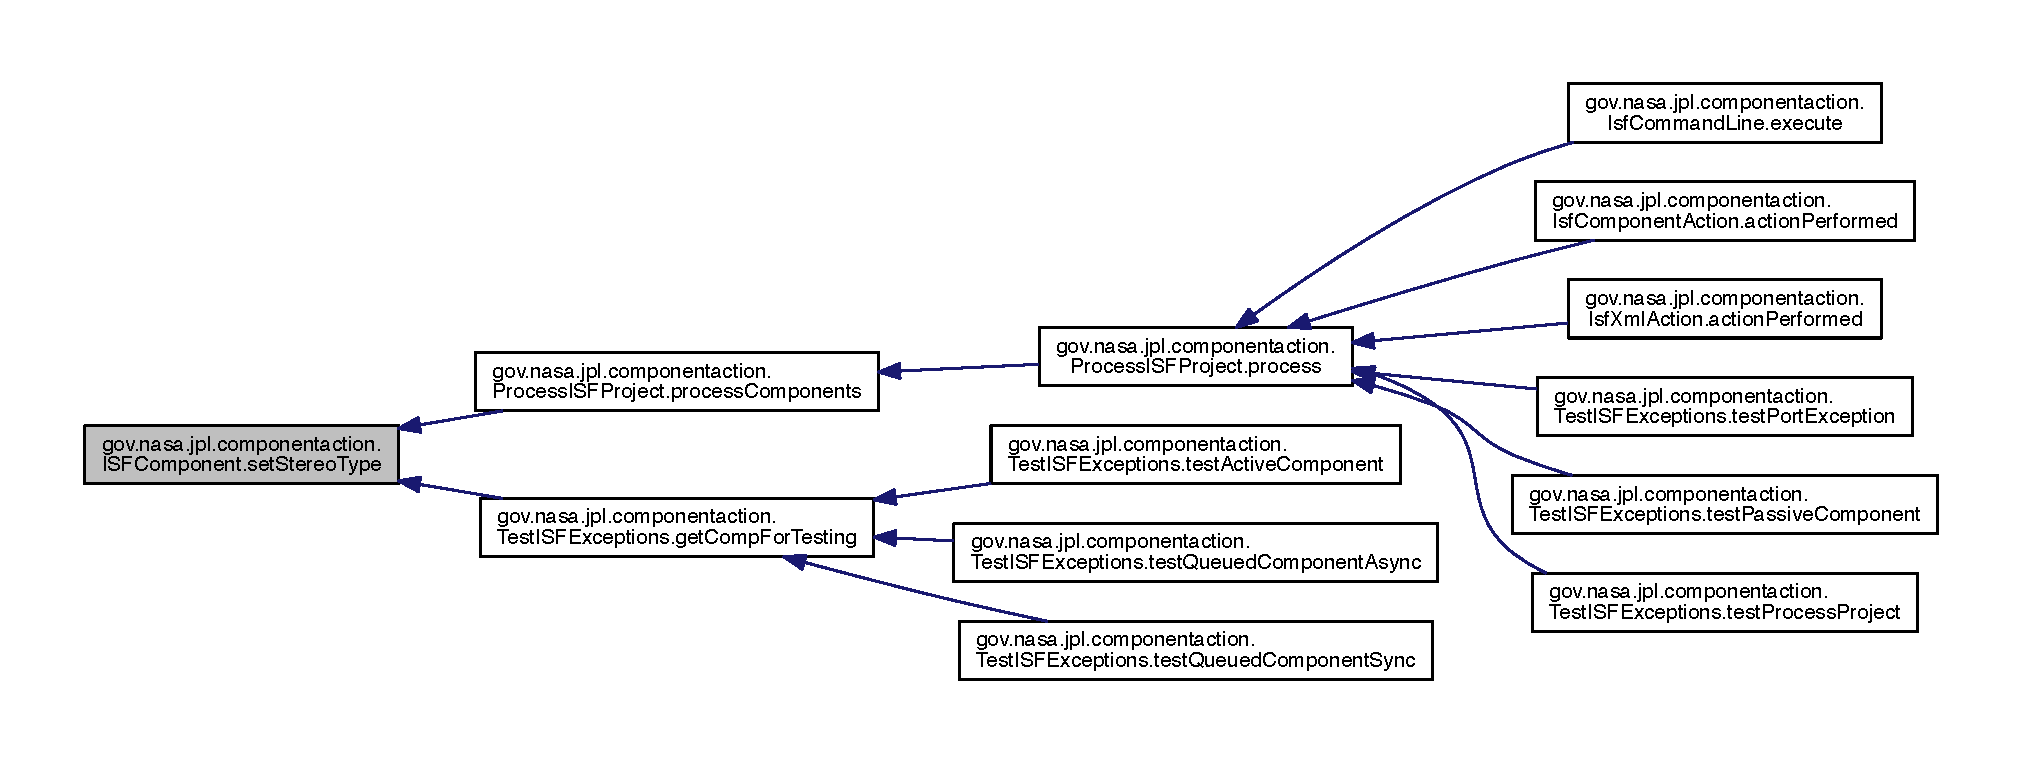
\includegraphics[width=350pt]{classgov_1_1nasa_1_1jpl_1_1componentaction_1_1_i_s_f_component_ac9317d03a2dcd968d3fa39f5a92bd350_icgraph}
\end{center}
\end{figure}


\index{gov\+::nasa\+::jpl\+::componentaction\+::\+I\+S\+F\+Component@{gov\+::nasa\+::jpl\+::componentaction\+::\+I\+S\+F\+Component}!warn\+Log@{warn\+Log}}
\index{warn\+Log@{warn\+Log}!gov\+::nasa\+::jpl\+::componentaction\+::\+I\+S\+F\+Component@{gov\+::nasa\+::jpl\+::componentaction\+::\+I\+S\+F\+Component}}
\subsubsection[{warn\+Log(\+String err\+Str)}]{\setlength{\rightskip}{0pt plus 5cm}void gov.\+nasa.\+jpl.\+componentaction.\+I\+S\+F\+Component.\+warn\+Log (
\begin{DoxyParamCaption}
\item[{String}]{err\+Str}
\end{DoxyParamCaption}
)}\label{classgov_1_1nasa_1_1jpl_1_1componentaction_1_1_i_s_f_component_a5a3939dfac9e1dbd1cd698091c00ebe2}
Prints a warning to the Java standard out as well as the Magic\+Draw console. 
\begin{DoxyParams}{Parameters}
{\em err\+Str} & Message to be printed \\
\hline
\end{DoxyParams}


\subsection{Member Data Documentation}
\index{gov\+::nasa\+::jpl\+::componentaction\+::\+I\+S\+F\+Component@{gov\+::nasa\+::jpl\+::componentaction\+::\+I\+S\+F\+Component}!component\+Element@{component\+Element}}
\index{component\+Element@{component\+Element}!gov\+::nasa\+::jpl\+::componentaction\+::\+I\+S\+F\+Component@{gov\+::nasa\+::jpl\+::componentaction\+::\+I\+S\+F\+Component}}
\subsubsection[{component\+Element}]{\setlength{\rightskip}{0pt plus 5cm}Element gov.\+nasa.\+jpl.\+componentaction.\+I\+S\+F\+Component.\+component\+Element\hspace{0.3cm}{\ttfamily [private]}}\label{classgov_1_1nasa_1_1jpl_1_1componentaction_1_1_i_s_f_component_af393209e66e60485577c2dc05fd8d67b}
\index{gov\+::nasa\+::jpl\+::componentaction\+::\+I\+S\+F\+Component@{gov\+::nasa\+::jpl\+::componentaction\+::\+I\+S\+F\+Component}!comp\+Stereotype@{comp\+Stereotype}}
\index{comp\+Stereotype@{comp\+Stereotype}!gov\+::nasa\+::jpl\+::componentaction\+::\+I\+S\+F\+Component@{gov\+::nasa\+::jpl\+::componentaction\+::\+I\+S\+F\+Component}}
\subsubsection[{comp\+Stereotype}]{\setlength{\rightskip}{0pt plus 5cm}String gov.\+nasa.\+jpl.\+componentaction.\+I\+S\+F\+Component.\+comp\+Stereotype\hspace{0.3cm}{\ttfamily [private]}}\label{classgov_1_1nasa_1_1jpl_1_1componentaction_1_1_i_s_f_component_aa4bb97ec50d1e4e186010917a5b011fc}
\index{gov\+::nasa\+::jpl\+::componentaction\+::\+I\+S\+F\+Component@{gov\+::nasa\+::jpl\+::componentaction\+::\+I\+S\+F\+Component}!filt\+List@{filt\+List}}
\index{filt\+List@{filt\+List}!gov\+::nasa\+::jpl\+::componentaction\+::\+I\+S\+F\+Component@{gov\+::nasa\+::jpl\+::componentaction\+::\+I\+S\+F\+Component}}
\subsubsection[{filt\+List}]{\setlength{\rightskip}{0pt plus 5cm}Hash\+Map$<$String, {\bf port\+Object}$>$ gov.\+nasa.\+jpl.\+componentaction.\+I\+S\+F\+Component.\+filt\+List\hspace{0.3cm}{\ttfamily [package]}}\label{classgov_1_1nasa_1_1jpl_1_1componentaction_1_1_i_s_f_component_ae5b8ab004d60ef84d3df3099b6641e61}
\index{gov\+::nasa\+::jpl\+::componentaction\+::\+I\+S\+F\+Component@{gov\+::nasa\+::jpl\+::componentaction\+::\+I\+S\+F\+Component}!Include\+Cmd\+X\+ML@{Include\+Cmd\+X\+ML}}
\index{Include\+Cmd\+X\+ML@{Include\+Cmd\+X\+ML}!gov\+::nasa\+::jpl\+::componentaction\+::\+I\+S\+F\+Component@{gov\+::nasa\+::jpl\+::componentaction\+::\+I\+S\+F\+Component}}
\subsubsection[{Include\+Cmd\+X\+ML}]{\setlength{\rightskip}{0pt plus 5cm}String gov.\+nasa.\+jpl.\+componentaction.\+I\+S\+F\+Component.\+Include\+Cmd\+X\+ML\hspace{0.3cm}{\ttfamily [package]}}\label{classgov_1_1nasa_1_1jpl_1_1componentaction_1_1_i_s_f_component_a203d1ed8b72e4c3b43aa2cd8217d1a47}
\index{gov\+::nasa\+::jpl\+::componentaction\+::\+I\+S\+F\+Component@{gov\+::nasa\+::jpl\+::componentaction\+::\+I\+S\+F\+Component}!Include\+Evr\+X\+ML@{Include\+Evr\+X\+ML}}
\index{Include\+Evr\+X\+ML@{Include\+Evr\+X\+ML}!gov\+::nasa\+::jpl\+::componentaction\+::\+I\+S\+F\+Component@{gov\+::nasa\+::jpl\+::componentaction\+::\+I\+S\+F\+Component}}
\subsubsection[{Include\+Evr\+X\+ML}]{\setlength{\rightskip}{0pt plus 5cm}String gov.\+nasa.\+jpl.\+componentaction.\+I\+S\+F\+Component.\+Include\+Evr\+X\+ML\hspace{0.3cm}{\ttfamily [package]}}\label{classgov_1_1nasa_1_1jpl_1_1componentaction_1_1_i_s_f_component_a3c28897130c05c3277fe2e6800796704}
\index{gov\+::nasa\+::jpl\+::componentaction\+::\+I\+S\+F\+Component@{gov\+::nasa\+::jpl\+::componentaction\+::\+I\+S\+F\+Component}!Include\+Include\+Hdr@{Include\+Include\+Hdr}}
\index{Include\+Include\+Hdr@{Include\+Include\+Hdr}!gov\+::nasa\+::jpl\+::componentaction\+::\+I\+S\+F\+Component@{gov\+::nasa\+::jpl\+::componentaction\+::\+I\+S\+F\+Component}}
\subsubsection[{Include\+Include\+Hdr}]{\setlength{\rightskip}{0pt plus 5cm}String gov.\+nasa.\+jpl.\+componentaction.\+I\+S\+F\+Component.\+Include\+Include\+Hdr\hspace{0.3cm}{\ttfamily [package]}}\label{classgov_1_1nasa_1_1jpl_1_1componentaction_1_1_i_s_f_component_acc7fdc4a70c54f4dcddbdd3257c5699a}
\index{gov\+::nasa\+::jpl\+::componentaction\+::\+I\+S\+F\+Component@{gov\+::nasa\+::jpl\+::componentaction\+::\+I\+S\+F\+Component}!Include\+Internal\+I\+F\+X\+ML@{Include\+Internal\+I\+F\+X\+ML}}
\index{Include\+Internal\+I\+F\+X\+ML@{Include\+Internal\+I\+F\+X\+ML}!gov\+::nasa\+::jpl\+::componentaction\+::\+I\+S\+F\+Component@{gov\+::nasa\+::jpl\+::componentaction\+::\+I\+S\+F\+Component}}
\subsubsection[{Include\+Internal\+I\+F\+X\+ML}]{\setlength{\rightskip}{0pt plus 5cm}String gov.\+nasa.\+jpl.\+componentaction.\+I\+S\+F\+Component.\+Include\+Internal\+I\+F\+X\+ML\hspace{0.3cm}{\ttfamily [package]}}\label{classgov_1_1nasa_1_1jpl_1_1componentaction_1_1_i_s_f_component_ab83589e575c656785a1d7f2b7ab890a1}
\index{gov\+::nasa\+::jpl\+::componentaction\+::\+I\+S\+F\+Component@{gov\+::nasa\+::jpl\+::componentaction\+::\+I\+S\+F\+Component}!Include\+Param\+X\+ML@{Include\+Param\+X\+ML}}
\index{Include\+Param\+X\+ML@{Include\+Param\+X\+ML}!gov\+::nasa\+::jpl\+::componentaction\+::\+I\+S\+F\+Component@{gov\+::nasa\+::jpl\+::componentaction\+::\+I\+S\+F\+Component}}
\subsubsection[{Include\+Param\+X\+ML}]{\setlength{\rightskip}{0pt plus 5cm}String gov.\+nasa.\+jpl.\+componentaction.\+I\+S\+F\+Component.\+Include\+Param\+X\+ML\hspace{0.3cm}{\ttfamily [package]}}\label{classgov_1_1nasa_1_1jpl_1_1componentaction_1_1_i_s_f_component_a0a12f3e43e863af1203b542396c60c54}
\index{gov\+::nasa\+::jpl\+::componentaction\+::\+I\+S\+F\+Component@{gov\+::nasa\+::jpl\+::componentaction\+::\+I\+S\+F\+Component}!Include\+Tlm\+X\+ML@{Include\+Tlm\+X\+ML}}
\index{Include\+Tlm\+X\+ML@{Include\+Tlm\+X\+ML}!gov\+::nasa\+::jpl\+::componentaction\+::\+I\+S\+F\+Component@{gov\+::nasa\+::jpl\+::componentaction\+::\+I\+S\+F\+Component}}
\subsubsection[{Include\+Tlm\+X\+ML}]{\setlength{\rightskip}{0pt plus 5cm}String gov.\+nasa.\+jpl.\+componentaction.\+I\+S\+F\+Component.\+Include\+Tlm\+X\+ML\hspace{0.3cm}{\ttfamily [package]}}\label{classgov_1_1nasa_1_1jpl_1_1componentaction_1_1_i_s_f_component_a799eea634f57c0fba9119cc50f7c8845}
\index{gov\+::nasa\+::jpl\+::componentaction\+::\+I\+S\+F\+Component@{gov\+::nasa\+::jpl\+::componentaction\+::\+I\+S\+F\+Component}!U\+R\+I\+Name@{U\+R\+I\+Name}}
\index{U\+R\+I\+Name@{U\+R\+I\+Name}!gov\+::nasa\+::jpl\+::componentaction\+::\+I\+S\+F\+Component@{gov\+::nasa\+::jpl\+::componentaction\+::\+I\+S\+F\+Component}}
\subsubsection[{U\+R\+I\+Name}]{\setlength{\rightskip}{0pt plus 5cm}String gov.\+nasa.\+jpl.\+componentaction.\+I\+S\+F\+Component.\+U\+R\+I\+Name\hspace{0.3cm}{\ttfamily [private]}}\label{classgov_1_1nasa_1_1jpl_1_1componentaction_1_1_i_s_f_component_ace343a71f7c24f1c08c9c11c861f9e2e}


The documentation for this class was generated from the following file\+:\begin{DoxyCompactItemize}
\item 
src/gov/nasa/jpl/componentaction/{\bf I\+S\+F\+Component.\+java}\end{DoxyCompactItemize}

\section{gov.\+nasa.\+jpl.\+componentaction.\+Isf\+Component\+Action Class Reference}
\label{classgov_1_1nasa_1_1jpl_1_1componentaction_1_1_isf_component_action}\index{gov.\+nasa.\+jpl.\+componentaction.\+Isf\+Component\+Action@{gov.\+nasa.\+jpl.\+componentaction.\+Isf\+Component\+Action}}


Inheritance diagram for gov.\+nasa.\+jpl.\+componentaction.\+Isf\+Component\+Action\+:
\nopagebreak
\begin{figure}[H]
\begin{center}
\leavevmode
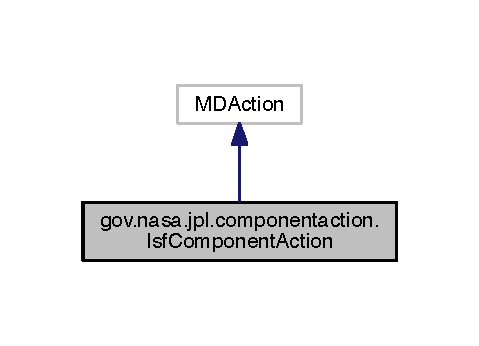
\includegraphics[width=230pt]{classgov_1_1nasa_1_1jpl_1_1componentaction_1_1_isf_component_action__inherit__graph}
\end{center}
\end{figure}


Collaboration diagram for gov.\+nasa.\+jpl.\+componentaction.\+Isf\+Component\+Action\+:
\nopagebreak
\begin{figure}[H]
\begin{center}
\leavevmode
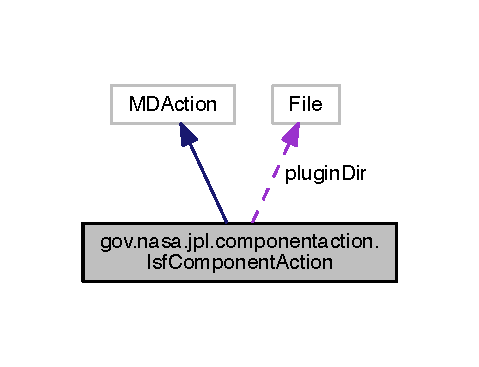
\includegraphics[width=230pt]{classgov_1_1nasa_1_1jpl_1_1componentaction_1_1_isf_component_action__coll__graph}
\end{center}
\end{figure}
\subsection*{Public Member Functions}
\begin{DoxyCompactItemize}
\item 
{\bf Isf\+Component\+Action} (String id, String name, File {\bf plugin\+Dir})
\item 
void {\bf action\+Performed} (Action\+Event e)
\end{DoxyCompactItemize}
\subsection*{Package Attributes}
\begin{DoxyCompactItemize}
\item 
File {\bf plugin\+Dir}
\end{DoxyCompactItemize}
\subsection*{Static Private Attributes}
\begin{DoxyCompactItemize}
\item 
static final long {\bf serial\+Version\+U\+ID} = -\/6790954285526957354L
\end{DoxyCompactItemize}


\subsection{Detailed Description}
Used to only generate Component and Port X\+ML diagrams. 

\subsection{Constructor \& Destructor Documentation}
\index{gov\+::nasa\+::jpl\+::componentaction\+::\+Isf\+Component\+Action@{gov\+::nasa\+::jpl\+::componentaction\+::\+Isf\+Component\+Action}!Isf\+Component\+Action@{Isf\+Component\+Action}}
\index{Isf\+Component\+Action@{Isf\+Component\+Action}!gov\+::nasa\+::jpl\+::componentaction\+::\+Isf\+Component\+Action@{gov\+::nasa\+::jpl\+::componentaction\+::\+Isf\+Component\+Action}}
\subsubsection[{Isf\+Component\+Action(\+String id, String name, File plugin\+Dir)}]{\setlength{\rightskip}{0pt plus 5cm}gov.\+nasa.\+jpl.\+componentaction.\+Isf\+Component\+Action.\+Isf\+Component\+Action (
\begin{DoxyParamCaption}
\item[{String}]{id, }
\item[{String}]{name, }
\item[{File}]{plugin\+Dir}
\end{DoxyParamCaption}
)}\label{classgov_1_1nasa_1_1jpl_1_1componentaction_1_1_isf_component_action_a6c3ddcc6f602920aa889e36e18769955}


\subsection{Member Function Documentation}
\index{gov\+::nasa\+::jpl\+::componentaction\+::\+Isf\+Component\+Action@{gov\+::nasa\+::jpl\+::componentaction\+::\+Isf\+Component\+Action}!action\+Performed@{action\+Performed}}
\index{action\+Performed@{action\+Performed}!gov\+::nasa\+::jpl\+::componentaction\+::\+Isf\+Component\+Action@{gov\+::nasa\+::jpl\+::componentaction\+::\+Isf\+Component\+Action}}
\subsubsection[{action\+Performed(\+Action\+Event e)}]{\setlength{\rightskip}{0pt plus 5cm}void gov.\+nasa.\+jpl.\+componentaction.\+Isf\+Component\+Action.\+action\+Performed (
\begin{DoxyParamCaption}
\item[{Action\+Event}]{e}
\end{DoxyParamCaption}
)}\label{classgov_1_1nasa_1_1jpl_1_1componentaction_1_1_isf_component_action_ab151441ea3f5c2c69ec198e7fdcd8159}
\begin{DoxySeeAlso}{See also}
java.\+awt.\+event.\+Action\+Listener\+::action\+Performed(java.\+awt.\+event.\+Action\+Event) 
\end{DoxySeeAlso}


Here is the call graph for this function\+:
\nopagebreak
\begin{figure}[H]
\begin{center}
\leavevmode
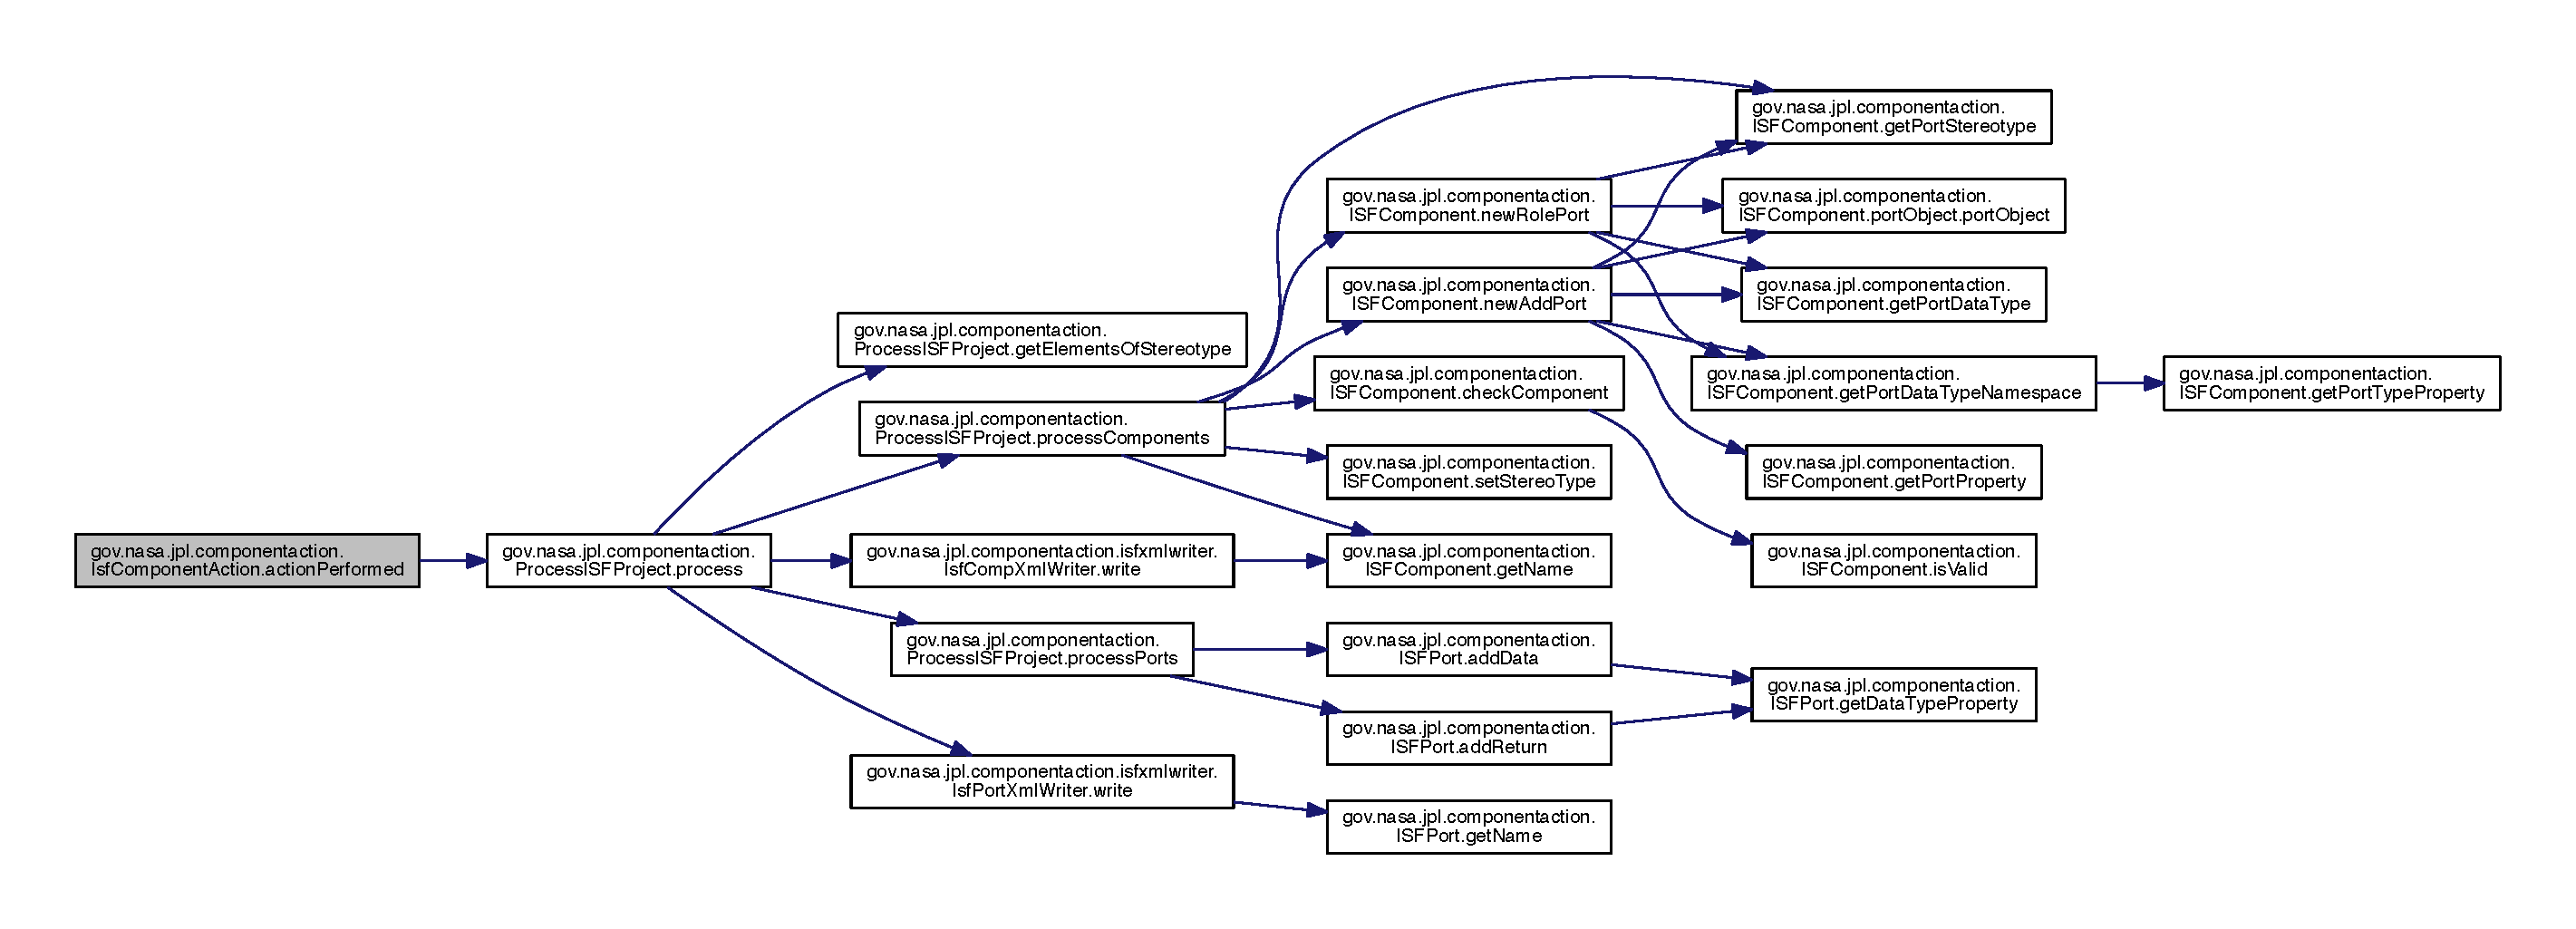
\includegraphics[width=350pt]{classgov_1_1nasa_1_1jpl_1_1componentaction_1_1_isf_component_action_ab151441ea3f5c2c69ec198e7fdcd8159_cgraph}
\end{center}
\end{figure}




\subsection{Member Data Documentation}
\index{gov\+::nasa\+::jpl\+::componentaction\+::\+Isf\+Component\+Action@{gov\+::nasa\+::jpl\+::componentaction\+::\+Isf\+Component\+Action}!plugin\+Dir@{plugin\+Dir}}
\index{plugin\+Dir@{plugin\+Dir}!gov\+::nasa\+::jpl\+::componentaction\+::\+Isf\+Component\+Action@{gov\+::nasa\+::jpl\+::componentaction\+::\+Isf\+Component\+Action}}
\subsubsection[{plugin\+Dir}]{\setlength{\rightskip}{0pt plus 5cm}File gov.\+nasa.\+jpl.\+componentaction.\+Isf\+Component\+Action.\+plugin\+Dir\hspace{0.3cm}{\ttfamily [package]}}\label{classgov_1_1nasa_1_1jpl_1_1componentaction_1_1_isf_component_action_a22369b6ea935d0afbdd583a66859fb4f}
\index{gov\+::nasa\+::jpl\+::componentaction\+::\+Isf\+Component\+Action@{gov\+::nasa\+::jpl\+::componentaction\+::\+Isf\+Component\+Action}!serial\+Version\+U\+ID@{serial\+Version\+U\+ID}}
\index{serial\+Version\+U\+ID@{serial\+Version\+U\+ID}!gov\+::nasa\+::jpl\+::componentaction\+::\+Isf\+Component\+Action@{gov\+::nasa\+::jpl\+::componentaction\+::\+Isf\+Component\+Action}}
\subsubsection[{serial\+Version\+U\+ID}]{\setlength{\rightskip}{0pt plus 5cm}final long gov.\+nasa.\+jpl.\+componentaction.\+Isf\+Component\+Action.\+serial\+Version\+U\+ID = -\/6790954285526957354L\hspace{0.3cm}{\ttfamily [static]}, {\ttfamily [private]}}\label{classgov_1_1nasa_1_1jpl_1_1componentaction_1_1_isf_component_action_a8632e4733aecfc2d4c17b5f2fff2e078}


The documentation for this class was generated from the following file\+:\begin{DoxyCompactItemize}
\item 
src/gov/nasa/jpl/componentaction/{\bf Isf\+Component\+Action.\+java}\end{DoxyCompactItemize}

\section{gov.\+nasa.\+jpl.\+componentaction.\+isfxmlwriter.\+Isf\+Comp\+Xml\+Writer Class Reference}
\label{classgov_1_1nasa_1_1jpl_1_1componentaction_1_1isfxmlwriter_1_1_isf_comp_xml_writer}\index{gov.\+nasa.\+jpl.\+componentaction.\+isfxmlwriter.\+Isf\+Comp\+Xml\+Writer@{gov.\+nasa.\+jpl.\+componentaction.\+isfxmlwriter.\+Isf\+Comp\+Xml\+Writer}}
\subsection*{Static Public Member Functions}
\begin{DoxyCompactItemize}
\item 
static void {\bf write} ({\bf I\+S\+F\+Component} comp, String file\+Name, String out\+Dir, File plugin\+Dir)
\end{DoxyCompactItemize}


\subsection{Member Function Documentation}
\index{gov\+::nasa\+::jpl\+::componentaction\+::isfxmlwriter\+::\+Isf\+Comp\+Xml\+Writer@{gov\+::nasa\+::jpl\+::componentaction\+::isfxmlwriter\+::\+Isf\+Comp\+Xml\+Writer}!write@{write}}
\index{write@{write}!gov\+::nasa\+::jpl\+::componentaction\+::isfxmlwriter\+::\+Isf\+Comp\+Xml\+Writer@{gov\+::nasa\+::jpl\+::componentaction\+::isfxmlwriter\+::\+Isf\+Comp\+Xml\+Writer}}
\subsubsection[{write(\+I\+S\+F\+Component comp, String file\+Name, String out\+Dir, File plugin\+Dir)}]{\setlength{\rightskip}{0pt plus 5cm}static void gov.\+nasa.\+jpl.\+componentaction.\+isfxmlwriter.\+Isf\+Comp\+Xml\+Writer.\+write (
\begin{DoxyParamCaption}
\item[{{\bf I\+S\+F\+Component}}]{comp, }
\item[{String}]{file\+Name, }
\item[{String}]{out\+Dir, }
\item[{File}]{plugin\+Dir}
\end{DoxyParamCaption}
)\hspace{0.3cm}{\ttfamily [static]}}\label{classgov_1_1nasa_1_1jpl_1_1componentaction_1_1isfxmlwriter_1_1_isf_comp_xml_writer_ac7914cd4b99539834e2f6e209612d5ec}
Writes the component X\+ML file. 

Here is the call graph for this function\+:
\nopagebreak
\begin{figure}[H]
\begin{center}
\leavevmode
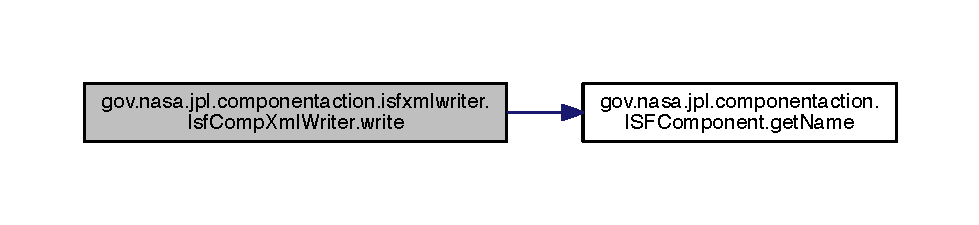
\includegraphics[width=350pt]{classgov_1_1nasa_1_1jpl_1_1componentaction_1_1isfxmlwriter_1_1_isf_comp_xml_writer_ac7914cd4b99539834e2f6e209612d5ec_cgraph}
\end{center}
\end{figure}




Here is the caller graph for this function\+:
\nopagebreak
\begin{figure}[H]
\begin{center}
\leavevmode
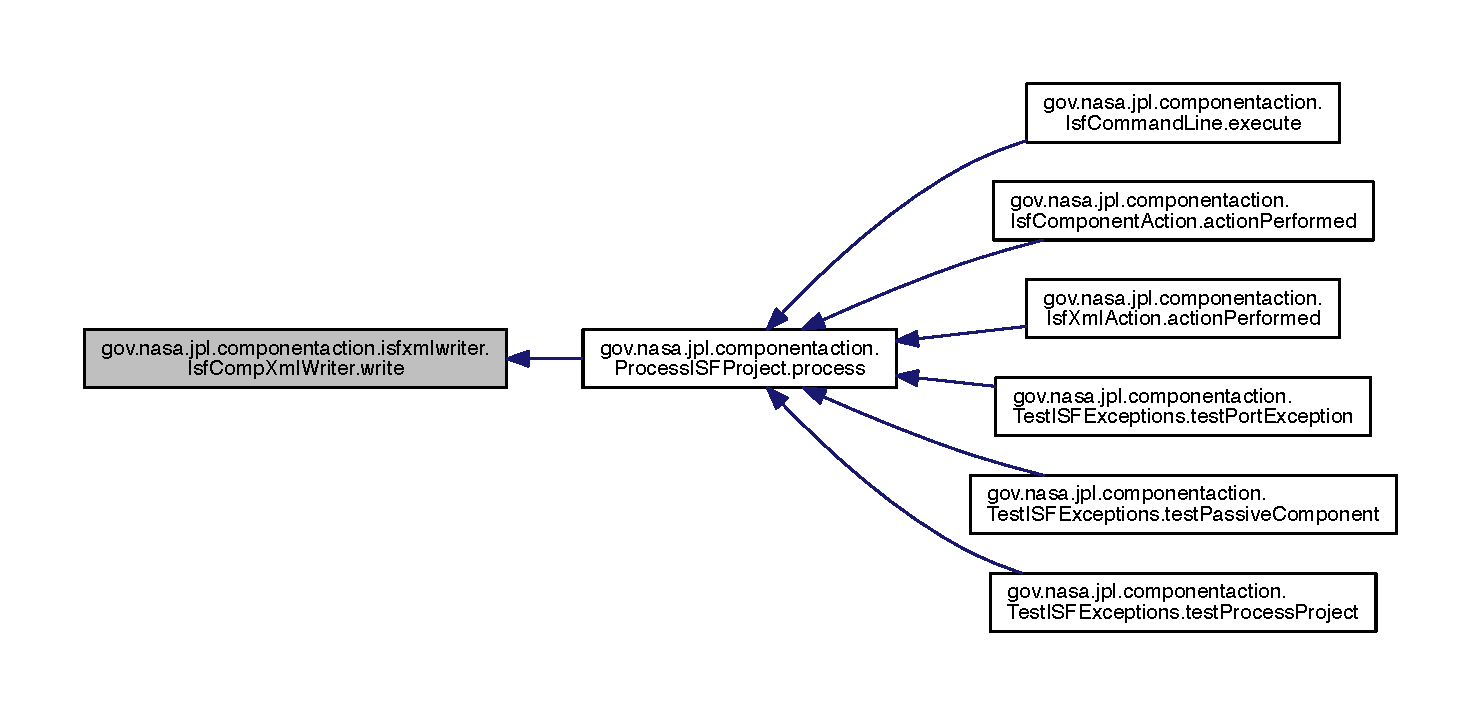
\includegraphics[width=350pt]{classgov_1_1nasa_1_1jpl_1_1componentaction_1_1isfxmlwriter_1_1_isf_comp_xml_writer_ac7914cd4b99539834e2f6e209612d5ec_icgraph}
\end{center}
\end{figure}




The documentation for this class was generated from the following file\+:\begin{DoxyCompactItemize}
\item 
src/gov/nasa/jpl/componentaction/isfxmlwriter/{\bf Isf\+Comp\+Xml\+Writer.\+java}\end{DoxyCompactItemize}

\section{gov.\+nasa.\+jpl.\+componentaction.\+I\+S\+F\+Port Class Reference}
\label{classgov_1_1nasa_1_1jpl_1_1componentaction_1_1_i_s_f_port}\index{gov.\+nasa.\+jpl.\+componentaction.\+I\+S\+F\+Port@{gov.\+nasa.\+jpl.\+componentaction.\+I\+S\+F\+Port}}


Collaboration diagram for gov.\+nasa.\+jpl.\+componentaction.\+I\+S\+F\+Port\+:
\nopagebreak
\begin{figure}[H]
\begin{center}
\leavevmode
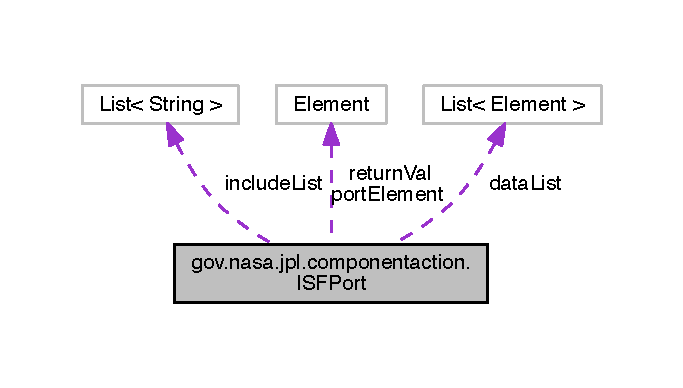
\includegraphics[width=328pt]{classgov_1_1nasa_1_1jpl_1_1componentaction_1_1_i_s_f_port__coll__graph}
\end{center}
\end{figure}
\subsection*{Public Member Functions}
\begin{DoxyCompactItemize}
\item 
{\bf I\+S\+F\+Port} (Element {\bf port\+Element})
\item 
String {\bf get\+Namespace} ()
\item 
void {\bf add\+Data} (Element data\+Element)
\item 
void {\bf add\+Return} (Element data\+Element)
\item 
boolean {\bf is\+Return\+Enumeration} (Element data\+Element)
\item 
boolean {\bf has\+Return} ()
\item 
Element {\bf get\+Return} ()
\item 
String {\bf get\+Return\+Type} (Element data\+Element)
\item 
String {\bf get\+Name} ()
\item 
String[$\,$] {\bf get\+Data\+Name} (Element data\+Element)
\item 
String {\bf get\+Data\+Type} (Element data\+Element)
\item 
List$<$ Element $>$ {\bf get\+Data\+List} ()
\item 
List$<$ String $>$ {\bf get\+Include\+List} ()
\item 
List$<$ Enumeration\+Literal $>$ {\bf get\+Enum\+Items} (Element data\+Element)
\item 
List$<$ Enumeration\+Literal $>$ {\bf get\+Return\+Enum\+Items} (Element data\+Element)
\item 
boolean {\bf is\+Enumeration} (Element data\+Element)
\item 
String {\bf get\+Port\+Type\+Property} (Element data\+Element, String property)
\item 
String {\bf get\+Data\+Type\+Property} (Element {\bf port\+Element}, String property)
\item 
void {\bf print} ()
\end{DoxyCompactItemize}
\subsection*{Private Attributes}
\begin{DoxyCompactItemize}
\item 
Element {\bf port\+Element}
\item 
List$<$ Element $>$ {\bf data\+List}
\item 
Element {\bf return\+Val}
\item 
List$<$ String $>$ {\bf include\+List}
\end{DoxyCompactItemize}


\subsection{Constructor \& Destructor Documentation}
\index{gov\+::nasa\+::jpl\+::componentaction\+::\+I\+S\+F\+Port@{gov\+::nasa\+::jpl\+::componentaction\+::\+I\+S\+F\+Port}!I\+S\+F\+Port@{I\+S\+F\+Port}}
\index{I\+S\+F\+Port@{I\+S\+F\+Port}!gov\+::nasa\+::jpl\+::componentaction\+::\+I\+S\+F\+Port@{gov\+::nasa\+::jpl\+::componentaction\+::\+I\+S\+F\+Port}}
\subsubsection[{I\+S\+F\+Port(\+Element port\+Element)}]{\setlength{\rightskip}{0pt plus 5cm}gov.\+nasa.\+jpl.\+componentaction.\+I\+S\+F\+Port.\+I\+S\+F\+Port (
\begin{DoxyParamCaption}
\item[{Element}]{port\+Element}
\end{DoxyParamCaption}
)}\label{classgov_1_1nasa_1_1jpl_1_1componentaction_1_1_i_s_f_port_aa1d42bf72de90d2f42d50bdd47cd299a}
Creates an \doxyref{I\+S\+F\+Port}{p.}{classgov_1_1nasa_1_1jpl_1_1componentaction_1_1_i_s_f_port} object 
\begin{DoxyParams}{Parameters}
{\em port\+Element} & Element of port type to be used in the creation of the object \\
\hline
\end{DoxyParams}


\subsection{Member Function Documentation}
\index{gov\+::nasa\+::jpl\+::componentaction\+::\+I\+S\+F\+Port@{gov\+::nasa\+::jpl\+::componentaction\+::\+I\+S\+F\+Port}!add\+Data@{add\+Data}}
\index{add\+Data@{add\+Data}!gov\+::nasa\+::jpl\+::componentaction\+::\+I\+S\+F\+Port@{gov\+::nasa\+::jpl\+::componentaction\+::\+I\+S\+F\+Port}}
\subsubsection[{add\+Data(\+Element data\+Element)}]{\setlength{\rightskip}{0pt plus 5cm}void gov.\+nasa.\+jpl.\+componentaction.\+I\+S\+F\+Port.\+add\+Data (
\begin{DoxyParamCaption}
\item[{Element}]{data\+Element}
\end{DoxyParamCaption}
)}\label{classgov_1_1nasa_1_1jpl_1_1componentaction_1_1_i_s_f_port_af5941e29cc1aa98d287f8679d31f9cbf}
Adds Element to the data\+List and checks to make sure the datatype is not empty before adding it to the include\+List. 
\begin{DoxyParams}{Parameters}
{\em data\+Element} & Element to be added \\
\hline
\end{DoxyParams}


Here is the call graph for this function\+:
\nopagebreak
\begin{figure}[H]
\begin{center}
\leavevmode
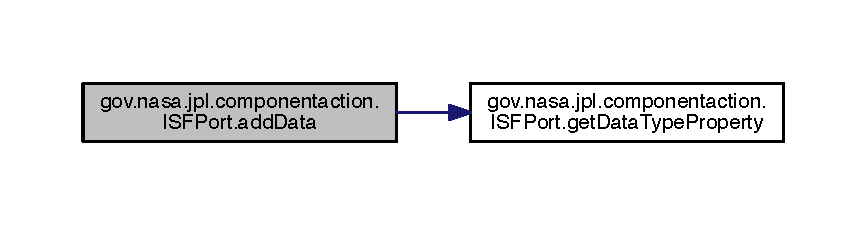
\includegraphics[width=350pt]{classgov_1_1nasa_1_1jpl_1_1componentaction_1_1_i_s_f_port_af5941e29cc1aa98d287f8679d31f9cbf_cgraph}
\end{center}
\end{figure}




Here is the caller graph for this function\+:
\nopagebreak
\begin{figure}[H]
\begin{center}
\leavevmode
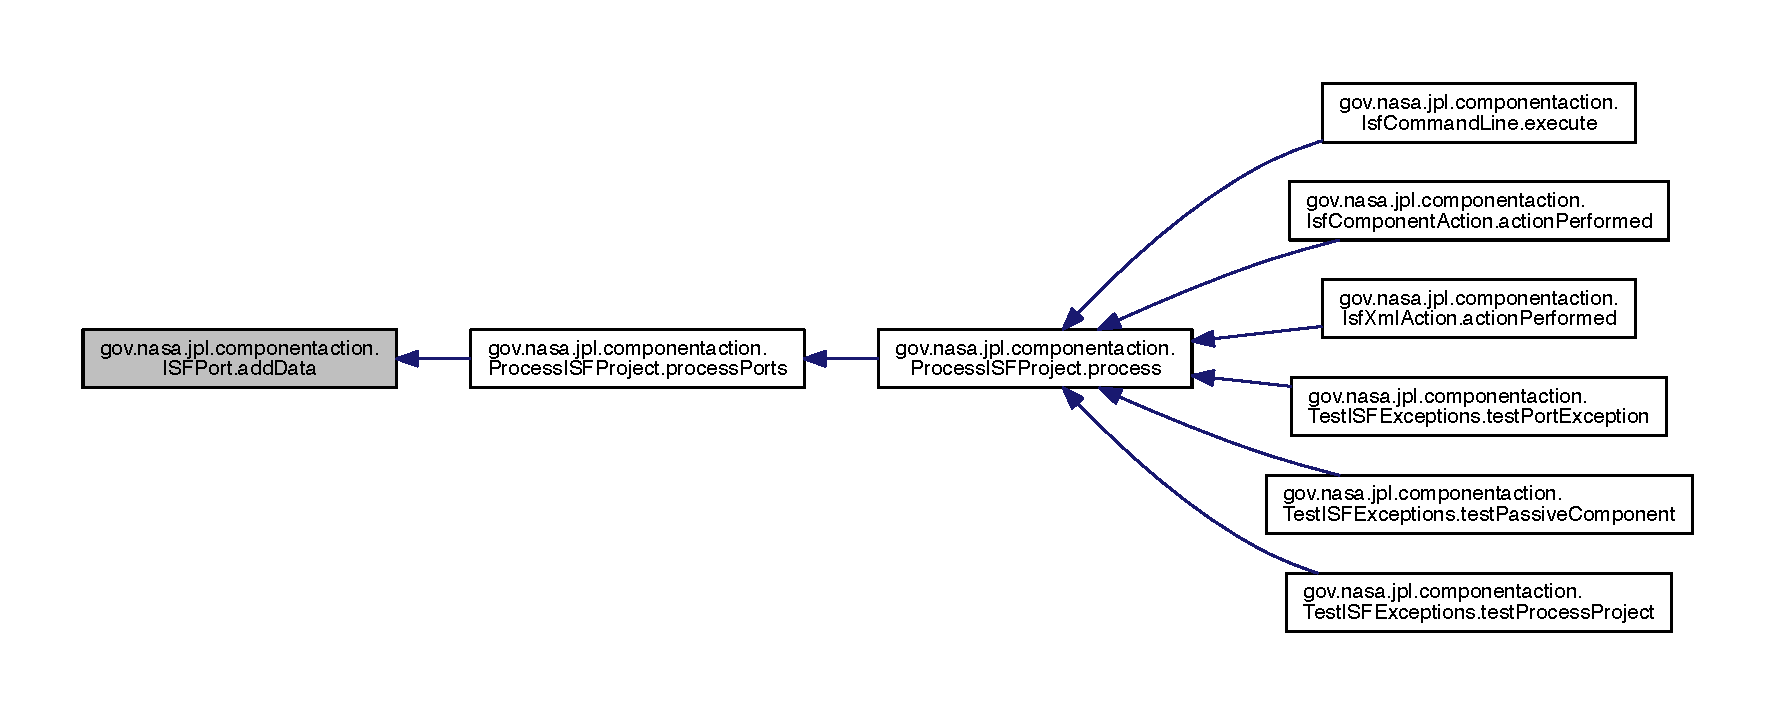
\includegraphics[width=350pt]{classgov_1_1nasa_1_1jpl_1_1componentaction_1_1_i_s_f_port_af5941e29cc1aa98d287f8679d31f9cbf_icgraph}
\end{center}
\end{figure}


\index{gov\+::nasa\+::jpl\+::componentaction\+::\+I\+S\+F\+Port@{gov\+::nasa\+::jpl\+::componentaction\+::\+I\+S\+F\+Port}!add\+Return@{add\+Return}}
\index{add\+Return@{add\+Return}!gov\+::nasa\+::jpl\+::componentaction\+::\+I\+S\+F\+Port@{gov\+::nasa\+::jpl\+::componentaction\+::\+I\+S\+F\+Port}}
\subsubsection[{add\+Return(\+Element data\+Element)}]{\setlength{\rightskip}{0pt plus 5cm}void gov.\+nasa.\+jpl.\+componentaction.\+I\+S\+F\+Port.\+add\+Return (
\begin{DoxyParamCaption}
\item[{Element}]{data\+Element}
\end{DoxyParamCaption}
)}\label{classgov_1_1nasa_1_1jpl_1_1componentaction_1_1_i_s_f_port_ab6952696e36b63b35e07c0b6d45c153d}
Adds Element to the include\+List if the datatype is not empty. 
\begin{DoxyParams}{Parameters}
{\em data\+Element} & \\
\hline
\end{DoxyParams}


Here is the call graph for this function\+:
\nopagebreak
\begin{figure}[H]
\begin{center}
\leavevmode
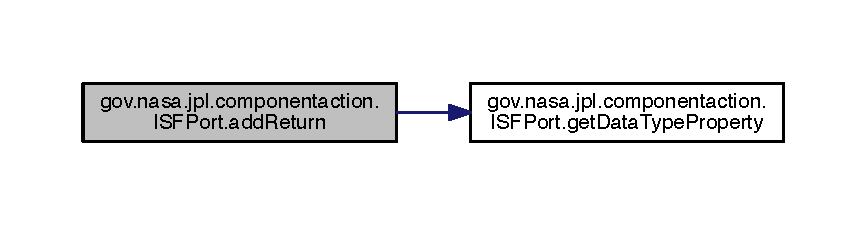
\includegraphics[width=350pt]{classgov_1_1nasa_1_1jpl_1_1componentaction_1_1_i_s_f_port_ab6952696e36b63b35e07c0b6d45c153d_cgraph}
\end{center}
\end{figure}




Here is the caller graph for this function\+:
\nopagebreak
\begin{figure}[H]
\begin{center}
\leavevmode
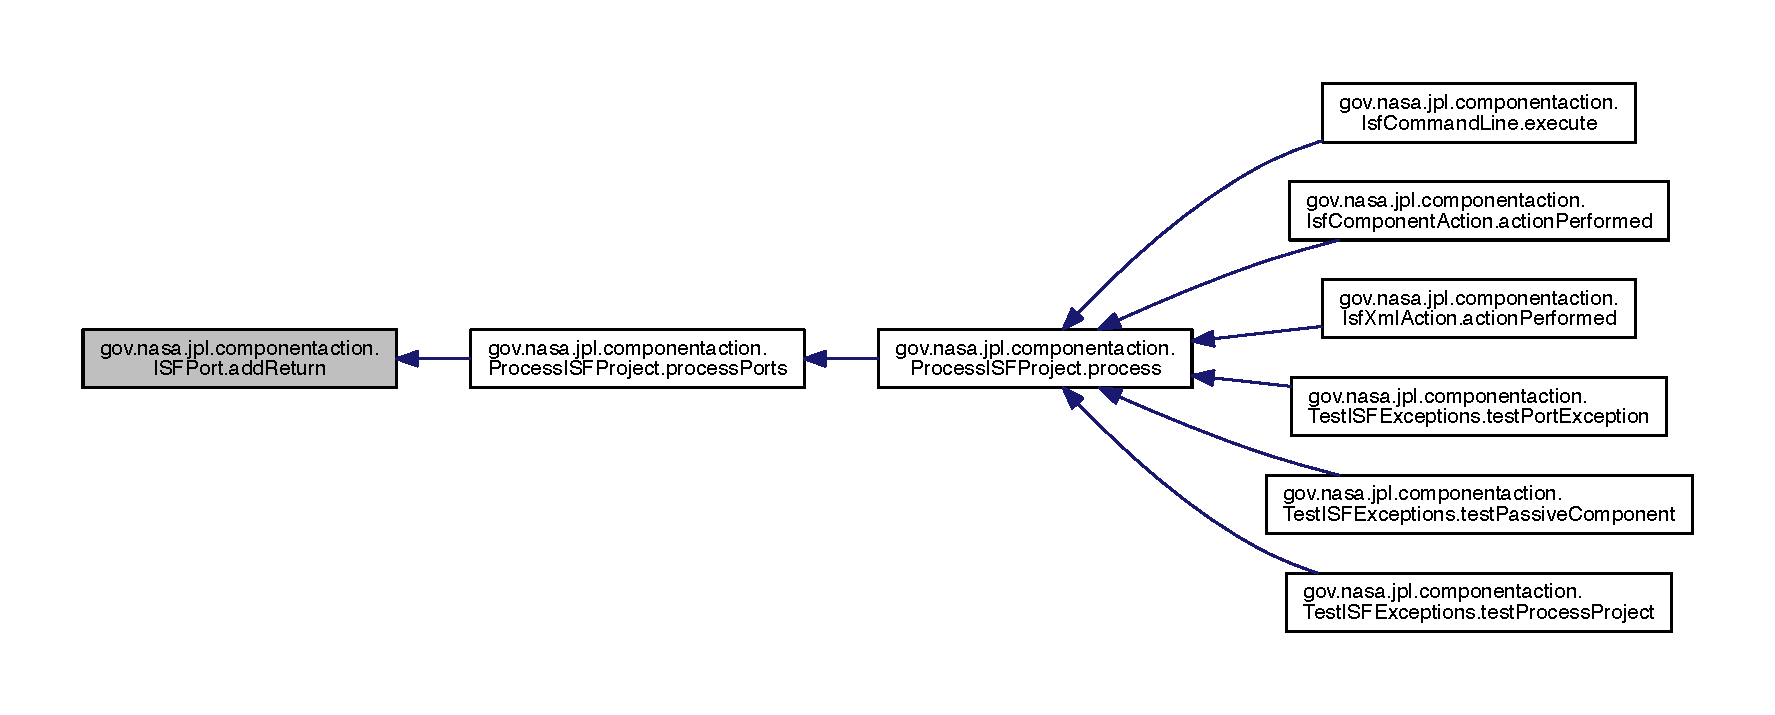
\includegraphics[width=350pt]{classgov_1_1nasa_1_1jpl_1_1componentaction_1_1_i_s_f_port_ab6952696e36b63b35e07c0b6d45c153d_icgraph}
\end{center}
\end{figure}


\index{gov\+::nasa\+::jpl\+::componentaction\+::\+I\+S\+F\+Port@{gov\+::nasa\+::jpl\+::componentaction\+::\+I\+S\+F\+Port}!get\+Data\+List@{get\+Data\+List}}
\index{get\+Data\+List@{get\+Data\+List}!gov\+::nasa\+::jpl\+::componentaction\+::\+I\+S\+F\+Port@{gov\+::nasa\+::jpl\+::componentaction\+::\+I\+S\+F\+Port}}
\subsubsection[{get\+Data\+List()}]{\setlength{\rightskip}{0pt plus 5cm}List$<$Element$>$ gov.\+nasa.\+jpl.\+componentaction.\+I\+S\+F\+Port.\+get\+Data\+List (
\begin{DoxyParamCaption}
{}
\end{DoxyParamCaption}
)}\label{classgov_1_1nasa_1_1jpl_1_1componentaction_1_1_i_s_f_port_ac5989d551d27c84011e9a0824ca535ef}
Returns the data\+L\+Ist \begin{DoxyReturn}{Returns}
List of Elements 
\end{DoxyReturn}
\index{gov\+::nasa\+::jpl\+::componentaction\+::\+I\+S\+F\+Port@{gov\+::nasa\+::jpl\+::componentaction\+::\+I\+S\+F\+Port}!get\+Data\+Name@{get\+Data\+Name}}
\index{get\+Data\+Name@{get\+Data\+Name}!gov\+::nasa\+::jpl\+::componentaction\+::\+I\+S\+F\+Port@{gov\+::nasa\+::jpl\+::componentaction\+::\+I\+S\+F\+Port}}
\subsubsection[{get\+Data\+Name(\+Element data\+Element)}]{\setlength{\rightskip}{0pt plus 5cm}String [$\,$] gov.\+nasa.\+jpl.\+componentaction.\+I\+S\+F\+Port.\+get\+Data\+Name (
\begin{DoxyParamCaption}
\item[{Element}]{data\+Element}
\end{DoxyParamCaption}
)}\label{classgov_1_1nasa_1_1jpl_1_1componentaction_1_1_i_s_f_port_a321f37c2d055d6c69aa4a70b0be18450}
Checks if the data\+Element is a reference or pointer and returns a list of Strings where the first value is the pass type and the second value is the name of the data\+Element. 
\begin{DoxyParams}{Parameters}
{\em data\+Element} & \\
\hline
\end{DoxyParams}
\begin{DoxyReturn}{Returns}
List of Strings 
\end{DoxyReturn}
\index{gov\+::nasa\+::jpl\+::componentaction\+::\+I\+S\+F\+Port@{gov\+::nasa\+::jpl\+::componentaction\+::\+I\+S\+F\+Port}!get\+Data\+Type@{get\+Data\+Type}}
\index{get\+Data\+Type@{get\+Data\+Type}!gov\+::nasa\+::jpl\+::componentaction\+::\+I\+S\+F\+Port@{gov\+::nasa\+::jpl\+::componentaction\+::\+I\+S\+F\+Port}}
\subsubsection[{get\+Data\+Type(\+Element data\+Element)}]{\setlength{\rightskip}{0pt plus 5cm}String gov.\+nasa.\+jpl.\+componentaction.\+I\+S\+F\+Port.\+get\+Data\+Type (
\begin{DoxyParamCaption}
\item[{Element}]{data\+Element}
\end{DoxyParamCaption}
)}\label{classgov_1_1nasa_1_1jpl_1_1componentaction_1_1_i_s_f_port_a774a8532b492e4ec5043d75af7169602}
Returns the data type with the namespace property prepended to it. 
\begin{DoxyParams}{Parameters}
{\em data\+Element} & \\
\hline
\end{DoxyParams}
\begin{DoxyReturn}{Returns}
namespace String 
\end{DoxyReturn}


Here is the call graph for this function\+:
\nopagebreak
\begin{figure}[H]
\begin{center}
\leavevmode
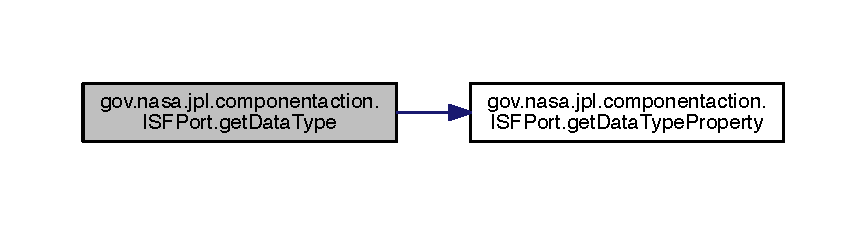
\includegraphics[width=350pt]{classgov_1_1nasa_1_1jpl_1_1componentaction_1_1_i_s_f_port_a774a8532b492e4ec5043d75af7169602_cgraph}
\end{center}
\end{figure}


\index{gov\+::nasa\+::jpl\+::componentaction\+::\+I\+S\+F\+Port@{gov\+::nasa\+::jpl\+::componentaction\+::\+I\+S\+F\+Port}!get\+Data\+Type\+Property@{get\+Data\+Type\+Property}}
\index{get\+Data\+Type\+Property@{get\+Data\+Type\+Property}!gov\+::nasa\+::jpl\+::componentaction\+::\+I\+S\+F\+Port@{gov\+::nasa\+::jpl\+::componentaction\+::\+I\+S\+F\+Port}}
\subsubsection[{get\+Data\+Type\+Property(\+Element port\+Element, String property)}]{\setlength{\rightskip}{0pt plus 5cm}String gov.\+nasa.\+jpl.\+componentaction.\+I\+S\+F\+Port.\+get\+Data\+Type\+Property (
\begin{DoxyParamCaption}
\item[{Element}]{port\+Element, }
\item[{String}]{property}
\end{DoxyParamCaption}
)}\label{classgov_1_1nasa_1_1jpl_1_1componentaction_1_1_i_s_f_port_a0043fd2665326ddb5fd6faf8a5f12608}
Returns the property value of Data\+Type stereotype of the input element argument.


\begin{DoxyParams}{Parameters}
{\em data\+Element} & The Element in question. \\
\hline
{\em property} & The parameter that is being accessed within the Data\+Type stereotype \\
\hline
\end{DoxyParams}
\begin{DoxyReturn}{Returns}
the associated value of the property in the Data\+Type stereotype 
\end{DoxyReturn}


Here is the caller graph for this function\+:
\nopagebreak
\begin{figure}[H]
\begin{center}
\leavevmode
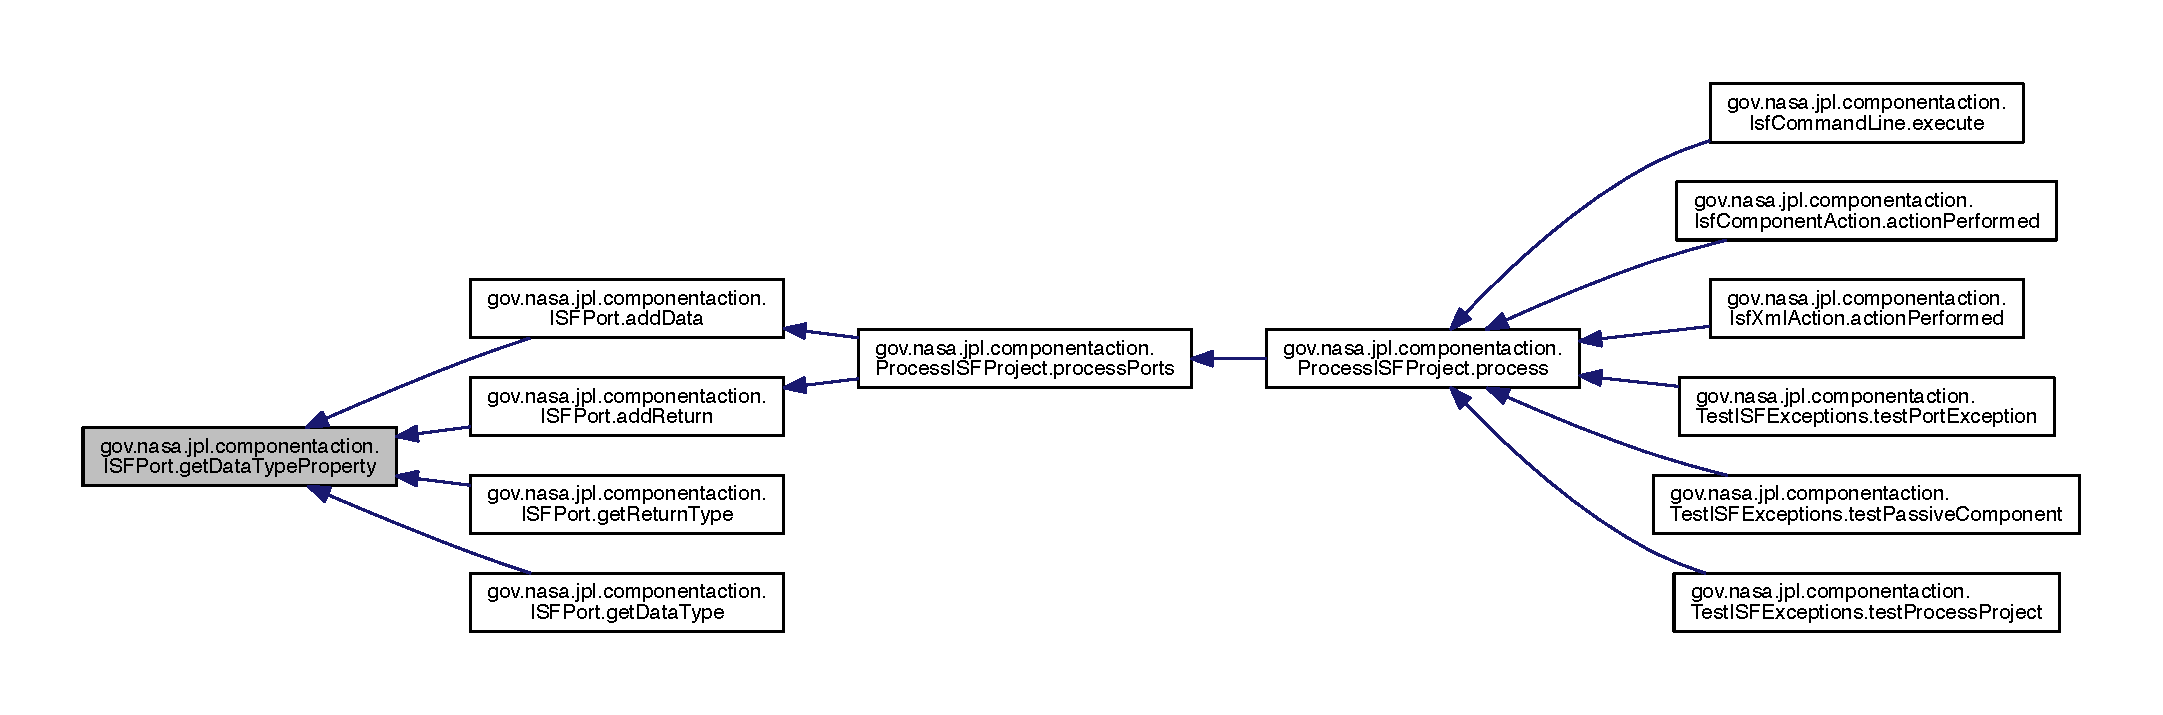
\includegraphics[width=350pt]{classgov_1_1nasa_1_1jpl_1_1componentaction_1_1_i_s_f_port_a0043fd2665326ddb5fd6faf8a5f12608_icgraph}
\end{center}
\end{figure}


\index{gov\+::nasa\+::jpl\+::componentaction\+::\+I\+S\+F\+Port@{gov\+::nasa\+::jpl\+::componentaction\+::\+I\+S\+F\+Port}!get\+Enum\+Items@{get\+Enum\+Items}}
\index{get\+Enum\+Items@{get\+Enum\+Items}!gov\+::nasa\+::jpl\+::componentaction\+::\+I\+S\+F\+Port@{gov\+::nasa\+::jpl\+::componentaction\+::\+I\+S\+F\+Port}}
\subsubsection[{get\+Enum\+Items(\+Element data\+Element)}]{\setlength{\rightskip}{0pt plus 5cm}List$<$Enumeration\+Literal$>$ gov.\+nasa.\+jpl.\+componentaction.\+I\+S\+F\+Port.\+get\+Enum\+Items (
\begin{DoxyParamCaption}
\item[{Element}]{data\+Element}
\end{DoxyParamCaption}
)}\label{classgov_1_1nasa_1_1jpl_1_1componentaction_1_1_i_s_f_port_a5f36ca8d2723e430936e05b3d8d46970}
Returns the enumerated items of the datatype. 
\begin{DoxyParams}{Parameters}
{\em data\+Element} & \\
\hline
\end{DoxyParams}
\begin{DoxyReturn}{Returns}
List of Enumeration Literal objects 
\end{DoxyReturn}
\index{gov\+::nasa\+::jpl\+::componentaction\+::\+I\+S\+F\+Port@{gov\+::nasa\+::jpl\+::componentaction\+::\+I\+S\+F\+Port}!get\+Include\+List@{get\+Include\+List}}
\index{get\+Include\+List@{get\+Include\+List}!gov\+::nasa\+::jpl\+::componentaction\+::\+I\+S\+F\+Port@{gov\+::nasa\+::jpl\+::componentaction\+::\+I\+S\+F\+Port}}
\subsubsection[{get\+Include\+List()}]{\setlength{\rightskip}{0pt plus 5cm}List$<$String$>$ gov.\+nasa.\+jpl.\+componentaction.\+I\+S\+F\+Port.\+get\+Include\+List (
\begin{DoxyParamCaption}
{}
\end{DoxyParamCaption}
)}\label{classgov_1_1nasa_1_1jpl_1_1componentaction_1_1_i_s_f_port_ae32a3fc2551597c3c651dca7d82bfc04}
Returns the include\+List \begin{DoxyReturn}{Returns}
List of Strings 
\end{DoxyReturn}
\index{gov\+::nasa\+::jpl\+::componentaction\+::\+I\+S\+F\+Port@{gov\+::nasa\+::jpl\+::componentaction\+::\+I\+S\+F\+Port}!get\+Name@{get\+Name}}
\index{get\+Name@{get\+Name}!gov\+::nasa\+::jpl\+::componentaction\+::\+I\+S\+F\+Port@{gov\+::nasa\+::jpl\+::componentaction\+::\+I\+S\+F\+Port}}
\subsubsection[{get\+Name()}]{\setlength{\rightskip}{0pt plus 5cm}String gov.\+nasa.\+jpl.\+componentaction.\+I\+S\+F\+Port.\+get\+Name (
\begin{DoxyParamCaption}
{}
\end{DoxyParamCaption}
)}\label{classgov_1_1nasa_1_1jpl_1_1componentaction_1_1_i_s_f_port_a58ab456c6f23017ab6d6b4d7b13a4a3c}
Returns the last part of the object name. \begin{DoxyReturn}{Returns}
String name 
\end{DoxyReturn}


Here is the caller graph for this function\+:
\nopagebreak
\begin{figure}[H]
\begin{center}
\leavevmode
\includegraphics[width=350pt]{classgov_1_1nasa_1_1jpl_1_1componentaction_1_1_i_s_f_port_a58ab456c6f23017ab6d6b4d7b13a4a3c_icgraph}
\end{center}
\end{figure}


\index{gov\+::nasa\+::jpl\+::componentaction\+::\+I\+S\+F\+Port@{gov\+::nasa\+::jpl\+::componentaction\+::\+I\+S\+F\+Port}!get\+Namespace@{get\+Namespace}}
\index{get\+Namespace@{get\+Namespace}!gov\+::nasa\+::jpl\+::componentaction\+::\+I\+S\+F\+Port@{gov\+::nasa\+::jpl\+::componentaction\+::\+I\+S\+F\+Port}}
\subsubsection[{get\+Namespace()}]{\setlength{\rightskip}{0pt plus 5cm}String gov.\+nasa.\+jpl.\+componentaction.\+I\+S\+F\+Port.\+get\+Namespace (
\begin{DoxyParamCaption}
{}
\end{DoxyParamCaption}
)}\label{classgov_1_1nasa_1_1jpl_1_1componentaction_1_1_i_s_f_port_af82251485fc2faa1ee991bfa84a5b8e3}
Return the port element\textquotesingle{}s namespace \begin{DoxyReturn}{Returns}
namespace string 
\end{DoxyReturn}


Here is the call graph for this function\+:
\nopagebreak
\begin{figure}[H]
\begin{center}
\leavevmode
\includegraphics[width=350pt]{classgov_1_1nasa_1_1jpl_1_1componentaction_1_1_i_s_f_port_af82251485fc2faa1ee991bfa84a5b8e3_cgraph}
\end{center}
\end{figure}


\index{gov\+::nasa\+::jpl\+::componentaction\+::\+I\+S\+F\+Port@{gov\+::nasa\+::jpl\+::componentaction\+::\+I\+S\+F\+Port}!get\+Port\+Type\+Property@{get\+Port\+Type\+Property}}
\index{get\+Port\+Type\+Property@{get\+Port\+Type\+Property}!gov\+::nasa\+::jpl\+::componentaction\+::\+I\+S\+F\+Port@{gov\+::nasa\+::jpl\+::componentaction\+::\+I\+S\+F\+Port}}
\subsubsection[{get\+Port\+Type\+Property(\+Element data\+Element, String property)}]{\setlength{\rightskip}{0pt plus 5cm}String gov.\+nasa.\+jpl.\+componentaction.\+I\+S\+F\+Port.\+get\+Port\+Type\+Property (
\begin{DoxyParamCaption}
\item[{Element}]{data\+Element, }
\item[{String}]{property}
\end{DoxyParamCaption}
)}\label{classgov_1_1nasa_1_1jpl_1_1componentaction_1_1_i_s_f_port_a1f65f30670687b662fecad76a3b3b1f5}
Returns the property value of the Port\+Type\textquotesingle{}s stereotype of the input element argument.


\begin{DoxyParams}{Parameters}
{\em data\+Element} & The Element in question. \\
\hline
{\em property} & The parameter that is being accessed within the Port\+Type stereotype \\
\hline
\end{DoxyParams}
\begin{DoxyReturn}{Returns}
the associated value of the property in the Port\+Type stereotype 
\end{DoxyReturn}


Here is the caller graph for this function\+:
\nopagebreak
\begin{figure}[H]
\begin{center}
\leavevmode
\includegraphics[width=350pt]{classgov_1_1nasa_1_1jpl_1_1componentaction_1_1_i_s_f_port_a1f65f30670687b662fecad76a3b3b1f5_icgraph}
\end{center}
\end{figure}


\index{gov\+::nasa\+::jpl\+::componentaction\+::\+I\+S\+F\+Port@{gov\+::nasa\+::jpl\+::componentaction\+::\+I\+S\+F\+Port}!get\+Return@{get\+Return}}
\index{get\+Return@{get\+Return}!gov\+::nasa\+::jpl\+::componentaction\+::\+I\+S\+F\+Port@{gov\+::nasa\+::jpl\+::componentaction\+::\+I\+S\+F\+Port}}
\subsubsection[{get\+Return()}]{\setlength{\rightskip}{0pt plus 5cm}Element gov.\+nasa.\+jpl.\+componentaction.\+I\+S\+F\+Port.\+get\+Return (
\begin{DoxyParamCaption}
{}
\end{DoxyParamCaption}
)}\label{classgov_1_1nasa_1_1jpl_1_1componentaction_1_1_i_s_f_port_a42de374af0eeec9562f8b0a3f8078c02}
Returns the return\+Val. \begin{DoxyReturn}{Returns}
return\+Val 
\end{DoxyReturn}
\index{gov\+::nasa\+::jpl\+::componentaction\+::\+I\+S\+F\+Port@{gov\+::nasa\+::jpl\+::componentaction\+::\+I\+S\+F\+Port}!get\+Return\+Enum\+Items@{get\+Return\+Enum\+Items}}
\index{get\+Return\+Enum\+Items@{get\+Return\+Enum\+Items}!gov\+::nasa\+::jpl\+::componentaction\+::\+I\+S\+F\+Port@{gov\+::nasa\+::jpl\+::componentaction\+::\+I\+S\+F\+Port}}
\subsubsection[{get\+Return\+Enum\+Items(\+Element data\+Element)}]{\setlength{\rightskip}{0pt plus 5cm}List$<$Enumeration\+Literal$>$ gov.\+nasa.\+jpl.\+componentaction.\+I\+S\+F\+Port.\+get\+Return\+Enum\+Items (
\begin{DoxyParamCaption}
\item[{Element}]{data\+Element}
\end{DoxyParamCaption}
)}\label{classgov_1_1nasa_1_1jpl_1_1componentaction_1_1_i_s_f_port_ae5dbe2a736bec807466d972760025448}
Get enumeration items from a Port\textquotesingle{}s Enumeration return type 
\begin{DoxyParams}{Parameters}
{\em data\+Element} & \\
\hline
\end{DoxyParams}
\begin{DoxyReturn}{Returns}

\end{DoxyReturn}
\index{gov\+::nasa\+::jpl\+::componentaction\+::\+I\+S\+F\+Port@{gov\+::nasa\+::jpl\+::componentaction\+::\+I\+S\+F\+Port}!get\+Return\+Type@{get\+Return\+Type}}
\index{get\+Return\+Type@{get\+Return\+Type}!gov\+::nasa\+::jpl\+::componentaction\+::\+I\+S\+F\+Port@{gov\+::nasa\+::jpl\+::componentaction\+::\+I\+S\+F\+Port}}
\subsubsection[{get\+Return\+Type(\+Element data\+Element)}]{\setlength{\rightskip}{0pt plus 5cm}String gov.\+nasa.\+jpl.\+componentaction.\+I\+S\+F\+Port.\+get\+Return\+Type (
\begin{DoxyParamCaption}
\item[{Element}]{data\+Element}
\end{DoxyParamCaption}
)}\label{classgov_1_1nasa_1_1jpl_1_1componentaction_1_1_i_s_f_port_af89c3bf4d933d4aedff46e58cb22b9b7}
Returns String based off the data\+Element. 
\begin{DoxyParams}{Parameters}
{\em data\+Element} & Input Element \\
\hline
\end{DoxyParams}
\begin{DoxyReturn}{Returns}
Return\+Type 
\end{DoxyReturn}


Here is the call graph for this function\+:
\nopagebreak
\begin{figure}[H]
\begin{center}
\leavevmode
\includegraphics[width=350pt]{classgov_1_1nasa_1_1jpl_1_1componentaction_1_1_i_s_f_port_af89c3bf4d933d4aedff46e58cb22b9b7_cgraph}
\end{center}
\end{figure}


\index{gov\+::nasa\+::jpl\+::componentaction\+::\+I\+S\+F\+Port@{gov\+::nasa\+::jpl\+::componentaction\+::\+I\+S\+F\+Port}!has\+Return@{has\+Return}}
\index{has\+Return@{has\+Return}!gov\+::nasa\+::jpl\+::componentaction\+::\+I\+S\+F\+Port@{gov\+::nasa\+::jpl\+::componentaction\+::\+I\+S\+F\+Port}}
\subsubsection[{has\+Return()}]{\setlength{\rightskip}{0pt plus 5cm}boolean gov.\+nasa.\+jpl.\+componentaction.\+I\+S\+F\+Port.\+has\+Return (
\begin{DoxyParamCaption}
{}
\end{DoxyParamCaption}
)}\label{classgov_1_1nasa_1_1jpl_1_1componentaction_1_1_i_s_f_port_a432cb07a3e3c12d7e290f94c85ff0fbf}
Checks if the return\+Val is null. \begin{DoxyReturn}{Returns}
True if the \doxyref{I\+S\+F\+Port}{p.}{classgov_1_1nasa_1_1jpl_1_1componentaction_1_1_i_s_f_port} has a return\+Value 
\end{DoxyReturn}
\index{gov\+::nasa\+::jpl\+::componentaction\+::\+I\+S\+F\+Port@{gov\+::nasa\+::jpl\+::componentaction\+::\+I\+S\+F\+Port}!is\+Enumeration@{is\+Enumeration}}
\index{is\+Enumeration@{is\+Enumeration}!gov\+::nasa\+::jpl\+::componentaction\+::\+I\+S\+F\+Port@{gov\+::nasa\+::jpl\+::componentaction\+::\+I\+S\+F\+Port}}
\subsubsection[{is\+Enumeration(\+Element data\+Element)}]{\setlength{\rightskip}{0pt plus 5cm}boolean gov.\+nasa.\+jpl.\+componentaction.\+I\+S\+F\+Port.\+is\+Enumeration (
\begin{DoxyParamCaption}
\item[{Element}]{data\+Element}
\end{DoxyParamCaption}
)}\label{classgov_1_1nasa_1_1jpl_1_1componentaction_1_1_i_s_f_port_a468c22dabd9405dbf4b4d3e6d9820cb6}
Checks if the Type of the data\+Element is an instance of Enumeration. 
\begin{DoxyParams}{Parameters}
{\em data\+Element} & \\
\hline
\end{DoxyParams}
\begin{DoxyReturn}{Returns}
boolean 
\end{DoxyReturn}
\index{gov\+::nasa\+::jpl\+::componentaction\+::\+I\+S\+F\+Port@{gov\+::nasa\+::jpl\+::componentaction\+::\+I\+S\+F\+Port}!is\+Return\+Enumeration@{is\+Return\+Enumeration}}
\index{is\+Return\+Enumeration@{is\+Return\+Enumeration}!gov\+::nasa\+::jpl\+::componentaction\+::\+I\+S\+F\+Port@{gov\+::nasa\+::jpl\+::componentaction\+::\+I\+S\+F\+Port}}
\subsubsection[{is\+Return\+Enumeration(\+Element data\+Element)}]{\setlength{\rightskip}{0pt plus 5cm}boolean gov.\+nasa.\+jpl.\+componentaction.\+I\+S\+F\+Port.\+is\+Return\+Enumeration (
\begin{DoxyParamCaption}
\item[{Element}]{data\+Element}
\end{DoxyParamCaption}
)}\label{classgov_1_1nasa_1_1jpl_1_1componentaction_1_1_i_s_f_port_a4631b0acd668f12386dcfa162e22f46b}
Checks if the Element object is an instance of Enumeration. 
\begin{DoxyParams}{Parameters}
{\em data\+Element} & Object to be checked \\
\hline
\end{DoxyParams}
\begin{DoxyReturn}{Returns}
True if the Element is an instance of Enumeration 
\end{DoxyReturn}
\index{gov\+::nasa\+::jpl\+::componentaction\+::\+I\+S\+F\+Port@{gov\+::nasa\+::jpl\+::componentaction\+::\+I\+S\+F\+Port}!print@{print}}
\index{print@{print}!gov\+::nasa\+::jpl\+::componentaction\+::\+I\+S\+F\+Port@{gov\+::nasa\+::jpl\+::componentaction\+::\+I\+S\+F\+Port}}
\subsubsection[{print()}]{\setlength{\rightskip}{0pt plus 5cm}void gov.\+nasa.\+jpl.\+componentaction.\+I\+S\+F\+Port.\+print (
\begin{DoxyParamCaption}
{}
\end{DoxyParamCaption}
)}\label{classgov_1_1nasa_1_1jpl_1_1componentaction_1_1_i_s_f_port_ac604b46eeb3997d52e0ba44514769820}
Prints the name of the I\+S\+Port object. 

Here is the call graph for this function\+:
\nopagebreak
\begin{figure}[H]
\begin{center}
\leavevmode
\includegraphics[width=350pt]{classgov_1_1nasa_1_1jpl_1_1componentaction_1_1_i_s_f_port_ac604b46eeb3997d52e0ba44514769820_cgraph}
\end{center}
\end{figure}




\subsection{Member Data Documentation}
\index{gov\+::nasa\+::jpl\+::componentaction\+::\+I\+S\+F\+Port@{gov\+::nasa\+::jpl\+::componentaction\+::\+I\+S\+F\+Port}!data\+List@{data\+List}}
\index{data\+List@{data\+List}!gov\+::nasa\+::jpl\+::componentaction\+::\+I\+S\+F\+Port@{gov\+::nasa\+::jpl\+::componentaction\+::\+I\+S\+F\+Port}}
\subsubsection[{data\+List}]{\setlength{\rightskip}{0pt plus 5cm}List$<$Element$>$ gov.\+nasa.\+jpl.\+componentaction.\+I\+S\+F\+Port.\+data\+List\hspace{0.3cm}{\ttfamily [private]}}\label{classgov_1_1nasa_1_1jpl_1_1componentaction_1_1_i_s_f_port_a823d8418ca16b03ccfee386e8a458b60}
\index{gov\+::nasa\+::jpl\+::componentaction\+::\+I\+S\+F\+Port@{gov\+::nasa\+::jpl\+::componentaction\+::\+I\+S\+F\+Port}!include\+List@{include\+List}}
\index{include\+List@{include\+List}!gov\+::nasa\+::jpl\+::componentaction\+::\+I\+S\+F\+Port@{gov\+::nasa\+::jpl\+::componentaction\+::\+I\+S\+F\+Port}}
\subsubsection[{include\+List}]{\setlength{\rightskip}{0pt plus 5cm}List$<$String$>$ gov.\+nasa.\+jpl.\+componentaction.\+I\+S\+F\+Port.\+include\+List\hspace{0.3cm}{\ttfamily [private]}}\label{classgov_1_1nasa_1_1jpl_1_1componentaction_1_1_i_s_f_port_ab1f5f73429cccf71feaba11ea137959a}
\index{gov\+::nasa\+::jpl\+::componentaction\+::\+I\+S\+F\+Port@{gov\+::nasa\+::jpl\+::componentaction\+::\+I\+S\+F\+Port}!port\+Element@{port\+Element}}
\index{port\+Element@{port\+Element}!gov\+::nasa\+::jpl\+::componentaction\+::\+I\+S\+F\+Port@{gov\+::nasa\+::jpl\+::componentaction\+::\+I\+S\+F\+Port}}
\subsubsection[{port\+Element}]{\setlength{\rightskip}{0pt plus 5cm}Element gov.\+nasa.\+jpl.\+componentaction.\+I\+S\+F\+Port.\+port\+Element\hspace{0.3cm}{\ttfamily [private]}}\label{classgov_1_1nasa_1_1jpl_1_1componentaction_1_1_i_s_f_port_a5653138b96da8f81a41f27e6e6f37b02}
\index{gov\+::nasa\+::jpl\+::componentaction\+::\+I\+S\+F\+Port@{gov\+::nasa\+::jpl\+::componentaction\+::\+I\+S\+F\+Port}!return\+Val@{return\+Val}}
\index{return\+Val@{return\+Val}!gov\+::nasa\+::jpl\+::componentaction\+::\+I\+S\+F\+Port@{gov\+::nasa\+::jpl\+::componentaction\+::\+I\+S\+F\+Port}}
\subsubsection[{return\+Val}]{\setlength{\rightskip}{0pt plus 5cm}Element gov.\+nasa.\+jpl.\+componentaction.\+I\+S\+F\+Port.\+return\+Val\hspace{0.3cm}{\ttfamily [private]}}\label{classgov_1_1nasa_1_1jpl_1_1componentaction_1_1_i_s_f_port_abdb898e35756b6055d59b58df01c0378}


The documentation for this class was generated from the following file\+:\begin{DoxyCompactItemize}
\item 
src/gov/nasa/jpl/componentaction/{\bf I\+S\+F\+Port.\+java}\end{DoxyCompactItemize}

\section{gov.\+nasa.\+jpl.\+componentaction.\+isfxmlwriter.\+Isf\+Port\+Xml\+Writer Class Reference}
\label{classgov_1_1nasa_1_1jpl_1_1componentaction_1_1isfxmlwriter_1_1_isf_port_xml_writer}\index{gov.\+nasa.\+jpl.\+componentaction.\+isfxmlwriter.\+Isf\+Port\+Xml\+Writer@{gov.\+nasa.\+jpl.\+componentaction.\+isfxmlwriter.\+Isf\+Port\+Xml\+Writer}}
\subsection*{Static Public Member Functions}
\begin{DoxyCompactItemize}
\item 
static void {\bf write} ({\bf I\+S\+F\+Port} port, String file\+Name, String out\+Dir, File plugin\+Dir)
\end{DoxyCompactItemize}


\subsection{Member Function Documentation}
\index{gov\+::nasa\+::jpl\+::componentaction\+::isfxmlwriter\+::\+Isf\+Port\+Xml\+Writer@{gov\+::nasa\+::jpl\+::componentaction\+::isfxmlwriter\+::\+Isf\+Port\+Xml\+Writer}!write@{write}}
\index{write@{write}!gov\+::nasa\+::jpl\+::componentaction\+::isfxmlwriter\+::\+Isf\+Port\+Xml\+Writer@{gov\+::nasa\+::jpl\+::componentaction\+::isfxmlwriter\+::\+Isf\+Port\+Xml\+Writer}}
\subsubsection[{write(\+I\+S\+F\+Port port, String file\+Name, String out\+Dir, File plugin\+Dir)}]{\setlength{\rightskip}{0pt plus 5cm}static void gov.\+nasa.\+jpl.\+componentaction.\+isfxmlwriter.\+Isf\+Port\+Xml\+Writer.\+write (
\begin{DoxyParamCaption}
\item[{{\bf I\+S\+F\+Port}}]{port, }
\item[{String}]{file\+Name, }
\item[{String}]{out\+Dir, }
\item[{File}]{plugin\+Dir}
\end{DoxyParamCaption}
)\hspace{0.3cm}{\ttfamily [static]}}\label{classgov_1_1nasa_1_1jpl_1_1componentaction_1_1isfxmlwriter_1_1_isf_port_xml_writer_a6f5cbcab76d8872a8be33d4f9eb764c5}
Writes the Port X\+ML files. 
\begin{DoxyParams}{Parameters}
{\em port} & \\
\hline
{\em file\+Name} & \\
\hline
{\em out\+Dir} & \\
\hline
{\em plugin\+Dir} & \\
\hline
\end{DoxyParams}


Here is the call graph for this function\+:
\nopagebreak
\begin{figure}[H]
\begin{center}
\leavevmode
\includegraphics[width=350pt]{classgov_1_1nasa_1_1jpl_1_1componentaction_1_1isfxmlwriter_1_1_isf_port_xml_writer_a6f5cbcab76d8872a8be33d4f9eb764c5_cgraph}
\end{center}
\end{figure}




Here is the caller graph for this function\+:
\nopagebreak
\begin{figure}[H]
\begin{center}
\leavevmode
\includegraphics[width=350pt]{classgov_1_1nasa_1_1jpl_1_1componentaction_1_1isfxmlwriter_1_1_isf_port_xml_writer_a6f5cbcab76d8872a8be33d4f9eb764c5_icgraph}
\end{center}
\end{figure}




The documentation for this class was generated from the following file\+:\begin{DoxyCompactItemize}
\item 
src/gov/nasa/jpl/componentaction/isfxmlwriter/{\bf Isf\+Port\+Xml\+Writer.\+java}\end{DoxyCompactItemize}

\section{gov.\+nasa.\+jpl.\+componentaction.\+I\+S\+F\+Subsystem Class Reference}
\label{classgov_1_1nasa_1_1jpl_1_1componentaction_1_1_i_s_f_subsystem}\index{gov.\+nasa.\+jpl.\+componentaction.\+I\+S\+F\+Subsystem@{gov.\+nasa.\+jpl.\+componentaction.\+I\+S\+F\+Subsystem}}
\subsection*{Classes}
\begin{DoxyCompactItemize}
\item 
class {\bf component\+Type}
\item 
class {\bf physical\+Connection\+Type}
\item 
class {\bf topology\+Model}
\end{DoxyCompactItemize}
\subsection*{Static Public Member Functions}
\begin{DoxyCompactItemize}
\item 
static {\bf component\+Type} {\bf create\+Component} (String name, String name\+Space, String type, String base\+ID, String instance\+Window, String xml\+Path)
\item 
static int {\bf get\+Source\+Index} (Connector conn)  throws Connector\+Exception 
\item 
static int {\bf get\+Target\+Index} (Connector conn)  throws Connector\+Exception 
\item 
static void {\bf print} ()
\item 
static String {\bf get\+File\+Location} (Element instance\+Element)
\item 
static String {\bf get\+Base\+Id} (Element instance\+Element)
\item 
static String {\bf get\+Instance\+Window} (Element instance\+Element)
\item 
static String {\bf get\+Source\+Comp} (Connector c)  throws Connector\+Exception 
\item 
static String {\bf get\+Target\+Comp} (Connector c)  throws Connector\+Exception 
\item 
static String {\bf get\+Comp\+Name} (Connector\+End conn)  throws Connector\+Exception 
\item 
static String {\bf get\+I\+D\+Source\+Port} (Connector c)  throws Connector\+Exception 
\item 
static String {\bf get\+I\+D\+Target\+Port} (Connector c)  throws Connector\+Exception 
\item 
static String {\bf get\+Source\+Port} (Connector c)  throws Connector\+Exception 
\item 
static String {\bf get\+Target\+Port} (Connector c)  throws Connector\+Exception 
\item 
static String {\bf get\+Port\+Name} (Connector\+End conn)  throws Connector\+Exception 
\item 
static String {\bf get\+Last\+Part\+Of\+String} (String in)
\item 
static String {\bf get\+Qualified\+Port} (Connector\+End conn\+End)
\item 
static String {\bf get\+Qualified\+Source\+Port} (Connector c)  throws Connector\+Exception 
\item 
static String {\bf get\+Qualified\+Target\+Port} (Connector c)  throws Connector\+Exception 
\item 
static String {\bf get\+Source\+Port\+Type} (Connector c)  throws Connector\+Exception 
\item 
static String {\bf get\+Target\+Port\+Type} (Connector c)  throws Connector\+Exception 
\item 
static Connector\+End {\bf get\+Source\+Conn\+End} (Connector c)  throws Connector\+Exception 
\item 
static Connector\+End {\bf get\+Target\+Conn\+End} (Connector c)  throws Connector\+Exception
\item 
static Connector\+End {\bf get\+Conn\+End} (Connector c, boolean is\+Source)  throws Connector\+Exception 
\item 
static List$<$ Element $>$ {\bf get\+Elements\+Of\+Stereotype} (String stereotype)
\item 
static String {\bf get\+Namespace} (Element component\+Element)
\end{DoxyCompactItemize}


\subsection{Detailed Description}
Helper class for \doxyref{Process\+I\+S\+F\+Topology}{p.}{classgov_1_1nasa_1_1jpl_1_1componentaction_1_1_process_i_s_f_topology} 

\subsection{Member Function Documentation}
\index{gov\+::nasa\+::jpl\+::componentaction\+::\+I\+S\+F\+Subsystem@{gov\+::nasa\+::jpl\+::componentaction\+::\+I\+S\+F\+Subsystem}!create\+Component@{create\+Component}}
\index{create\+Component@{create\+Component}!gov\+::nasa\+::jpl\+::componentaction\+::\+I\+S\+F\+Subsystem@{gov\+::nasa\+::jpl\+::componentaction\+::\+I\+S\+F\+Subsystem}}
\subsubsection[{create\+Component(\+String name, String name\+Space, String type, String base\+I\+D, String instance\+Window, String xml\+Path)}]{\setlength{\rightskip}{0pt plus 5cm}static {\bf component\+Type} gov.\+nasa.\+jpl.\+componentaction.\+I\+S\+F\+Subsystem.\+create\+Component (
\begin{DoxyParamCaption}
\item[{String}]{name, }
\item[{String}]{name\+Space, }
\item[{String}]{type, }
\item[{String}]{base\+ID, }
\item[{String}]{instance\+Window, }
\item[{String}]{xml\+Path}
\end{DoxyParamCaption}
)\hspace{0.3cm}{\ttfamily [static]}}\label{classgov_1_1nasa_1_1jpl_1_1componentaction_1_1_i_s_f_subsystem_a342939c55e428cdeb91d2a5d96040185}
Creates and returns new \doxyref{component\+Type}{p.}{classgov_1_1nasa_1_1jpl_1_1componentaction_1_1_i_s_f_subsystem_1_1component_type}


\begin{DoxyParams}{Parameters}
{\em name} & Component name \\
\hline
{\em name\+Space} & Component name space \\
\hline
{\em type} & Component Type \\
\hline
{\em base\+ID} & Base ID \\
\hline
{\em instance\+Window} & Instance Window ID \\
\hline
\end{DoxyParams}
\begin{DoxyReturn}{Returns}
\doxyref{component\+Type}{p.}{classgov_1_1nasa_1_1jpl_1_1componentaction_1_1_i_s_f_subsystem_1_1component_type} 
\end{DoxyReturn}


Here is the caller graph for this function\+:
\nopagebreak
\begin{figure}[H]
\begin{center}
\leavevmode
\includegraphics[width=350pt]{classgov_1_1nasa_1_1jpl_1_1componentaction_1_1_i_s_f_subsystem_a342939c55e428cdeb91d2a5d96040185_icgraph}
\end{center}
\end{figure}


\index{gov\+::nasa\+::jpl\+::componentaction\+::\+I\+S\+F\+Subsystem@{gov\+::nasa\+::jpl\+::componentaction\+::\+I\+S\+F\+Subsystem}!get\+Base\+Id@{get\+Base\+Id}}
\index{get\+Base\+Id@{get\+Base\+Id}!gov\+::nasa\+::jpl\+::componentaction\+::\+I\+S\+F\+Subsystem@{gov\+::nasa\+::jpl\+::componentaction\+::\+I\+S\+F\+Subsystem}}
\subsubsection[{get\+Base\+Id(\+Element instance\+Element)}]{\setlength{\rightskip}{0pt plus 5cm}static String gov.\+nasa.\+jpl.\+componentaction.\+I\+S\+F\+Subsystem.\+get\+Base\+Id (
\begin{DoxyParamCaption}
\item[{Element}]{instance\+Element}
\end{DoxyParamCaption}
)\hspace{0.3cm}{\ttfamily [static]}}\label{classgov_1_1nasa_1_1jpl_1_1componentaction_1_1_i_s_f_subsystem_a5c6980c26fbda08a7e930a1672daa4d2}
Returns the base ID of the element.


\begin{DoxyParams}{Parameters}
{\em instance\+Element} & \\
\hline
\end{DoxyParams}
\begin{DoxyReturn}{Returns}

\end{DoxyReturn}


Here is the caller graph for this function\+:
\nopagebreak
\begin{figure}[H]
\begin{center}
\leavevmode
\includegraphics[width=350pt]{classgov_1_1nasa_1_1jpl_1_1componentaction_1_1_i_s_f_subsystem_a5c6980c26fbda08a7e930a1672daa4d2_icgraph}
\end{center}
\end{figure}


\index{gov\+::nasa\+::jpl\+::componentaction\+::\+I\+S\+F\+Subsystem@{gov\+::nasa\+::jpl\+::componentaction\+::\+I\+S\+F\+Subsystem}!get\+Comp\+Name@{get\+Comp\+Name}}
\index{get\+Comp\+Name@{get\+Comp\+Name}!gov\+::nasa\+::jpl\+::componentaction\+::\+I\+S\+F\+Subsystem@{gov\+::nasa\+::jpl\+::componentaction\+::\+I\+S\+F\+Subsystem}}
\subsubsection[{get\+Comp\+Name(\+Connector\+End conn)}]{\setlength{\rightskip}{0pt plus 5cm}static String gov.\+nasa.\+jpl.\+componentaction.\+I\+S\+F\+Subsystem.\+get\+Comp\+Name (
\begin{DoxyParamCaption}
\item[{Connector\+End}]{conn}
\end{DoxyParamCaption}
) throws {\bf Connector\+Exception}\hspace{0.3cm}{\ttfamily [static]}}\label{classgov_1_1nasa_1_1jpl_1_1componentaction_1_1_i_s_f_subsystem_a4044ed4b73d4df7aa66400ac4057ce3c}
Returns the component name of the connector\+End. 
\begin{DoxyParams}{Parameters}
{\em conn} & \\
\hline
\end{DoxyParams}
\begin{DoxyReturn}{Returns}

\end{DoxyReturn}

\begin{DoxyExceptions}{Exceptions}
{\em \doxyref{Connector\+Exception}{p.}{classgov_1_1nasa_1_1jpl_1_1componentaction_1_1_connector_exception}} & \\
\hline
\end{DoxyExceptions}


Here is the caller graph for this function\+:
\nopagebreak
\begin{figure}[H]
\begin{center}
\leavevmode
\includegraphics[width=350pt]{classgov_1_1nasa_1_1jpl_1_1componentaction_1_1_i_s_f_subsystem_a4044ed4b73d4df7aa66400ac4057ce3c_icgraph}
\end{center}
\end{figure}


\index{gov\+::nasa\+::jpl\+::componentaction\+::\+I\+S\+F\+Subsystem@{gov\+::nasa\+::jpl\+::componentaction\+::\+I\+S\+F\+Subsystem}!get\+Conn\+End@{get\+Conn\+End}}
\index{get\+Conn\+End@{get\+Conn\+End}!gov\+::nasa\+::jpl\+::componentaction\+::\+I\+S\+F\+Subsystem@{gov\+::nasa\+::jpl\+::componentaction\+::\+I\+S\+F\+Subsystem}}
\subsubsection[{get\+Conn\+End(\+Connector c, boolean is\+Source)}]{\setlength{\rightskip}{0pt plus 5cm}static Connector\+End gov.\+nasa.\+jpl.\+componentaction.\+I\+S\+F\+Subsystem.\+get\+Conn\+End (
\begin{DoxyParamCaption}
\item[{Connector}]{c, }
\item[{boolean}]{is\+Source}
\end{DoxyParamCaption}
) throws {\bf Connector\+Exception}\hspace{0.3cm}{\ttfamily [static]}}\label{classgov_1_1nasa_1_1jpl_1_1componentaction_1_1_i_s_f_subsystem_a8d892025f44c008c6afd8c263ce6f458}
Both get\+Source\+Conn\+End and get\+Target\+Conn\+End use this function. Incorporates error handling/checking. 

The function checks the direction property of the first stereotype found in each port of the connector. Depending on what the connector can see within and around the system, the funcion will return what it sees as the source and what is sees as the target.


\begin{DoxyParams}{Parameters}
{\em c} & Connector \\
\hline
{\em is\+Source} & true if looking for source end, false if looking for target end \\
\hline
\end{DoxyParams}
\begin{DoxyReturn}{Returns}
Connector End 
\end{DoxyReturn}

\begin{DoxyExceptions}{Exceptions}
{\em \doxyref{Connector\+Exception}{p.}{classgov_1_1nasa_1_1jpl_1_1componentaction_1_1_connector_exception}} & \\
\hline
\end{DoxyExceptions}


Here is the call graph for this function\+:
\nopagebreak
\begin{figure}[H]
\begin{center}
\leavevmode
\includegraphics[width=350pt]{classgov_1_1nasa_1_1jpl_1_1componentaction_1_1_i_s_f_subsystem_a8d892025f44c008c6afd8c263ce6f458_cgraph}
\end{center}
\end{figure}




Here is the caller graph for this function\+:
\nopagebreak
\begin{figure}[H]
\begin{center}
\leavevmode
\includegraphics[width=350pt]{classgov_1_1nasa_1_1jpl_1_1componentaction_1_1_i_s_f_subsystem_a8d892025f44c008c6afd8c263ce6f458_icgraph}
\end{center}
\end{figure}


\index{gov\+::nasa\+::jpl\+::componentaction\+::\+I\+S\+F\+Subsystem@{gov\+::nasa\+::jpl\+::componentaction\+::\+I\+S\+F\+Subsystem}!get\+Elements\+Of\+Stereotype@{get\+Elements\+Of\+Stereotype}}
\index{get\+Elements\+Of\+Stereotype@{get\+Elements\+Of\+Stereotype}!gov\+::nasa\+::jpl\+::componentaction\+::\+I\+S\+F\+Subsystem@{gov\+::nasa\+::jpl\+::componentaction\+::\+I\+S\+F\+Subsystem}}
\subsubsection[{get\+Elements\+Of\+Stereotype(\+String stereotype)}]{\setlength{\rightskip}{0pt plus 5cm}static List$<$Element$>$ gov.\+nasa.\+jpl.\+componentaction.\+I\+S\+F\+Subsystem.\+get\+Elements\+Of\+Stereotype (
\begin{DoxyParamCaption}
\item[{String}]{stereotype}
\end{DoxyParamCaption}
)\hspace{0.3cm}{\ttfamily [static]}}\label{classgov_1_1nasa_1_1jpl_1_1componentaction_1_1_i_s_f_subsystem_aed6bbf8c9a1a92f40f3bdcef9e1cd8f5}
Returns a list of elements with the given stereotype String.


\begin{DoxyParams}{Parameters}
{\em stereotype} & String \\
\hline
\end{DoxyParams}
\begin{DoxyReturn}{Returns}
List of Objects 
\end{DoxyReturn}


Here is the caller graph for this function\+:
\nopagebreak
\begin{figure}[H]
\begin{center}
\leavevmode
\includegraphics[width=350pt]{classgov_1_1nasa_1_1jpl_1_1componentaction_1_1_i_s_f_subsystem_aed6bbf8c9a1a92f40f3bdcef9e1cd8f5_icgraph}
\end{center}
\end{figure}


\index{gov\+::nasa\+::jpl\+::componentaction\+::\+I\+S\+F\+Subsystem@{gov\+::nasa\+::jpl\+::componentaction\+::\+I\+S\+F\+Subsystem}!get\+File\+Location@{get\+File\+Location}}
\index{get\+File\+Location@{get\+File\+Location}!gov\+::nasa\+::jpl\+::componentaction\+::\+I\+S\+F\+Subsystem@{gov\+::nasa\+::jpl\+::componentaction\+::\+I\+S\+F\+Subsystem}}
\subsubsection[{get\+File\+Location(\+Element instance\+Element)}]{\setlength{\rightskip}{0pt plus 5cm}static String gov.\+nasa.\+jpl.\+componentaction.\+I\+S\+F\+Subsystem.\+get\+File\+Location (
\begin{DoxyParamCaption}
\item[{Element}]{instance\+Element}
\end{DoxyParamCaption}
)\hspace{0.3cm}{\ttfamily [static]}}\label{classgov_1_1nasa_1_1jpl_1_1componentaction_1_1_i_s_f_subsystem_ade10ca5d500a51c3f9f0c9835072b7e9}


Here is the caller graph for this function\+:
\nopagebreak
\begin{figure}[H]
\begin{center}
\leavevmode
\includegraphics[width=350pt]{classgov_1_1nasa_1_1jpl_1_1componentaction_1_1_i_s_f_subsystem_ade10ca5d500a51c3f9f0c9835072b7e9_icgraph}
\end{center}
\end{figure}


\index{gov\+::nasa\+::jpl\+::componentaction\+::\+I\+S\+F\+Subsystem@{gov\+::nasa\+::jpl\+::componentaction\+::\+I\+S\+F\+Subsystem}!get\+I\+D\+Source\+Port@{get\+I\+D\+Source\+Port}}
\index{get\+I\+D\+Source\+Port@{get\+I\+D\+Source\+Port}!gov\+::nasa\+::jpl\+::componentaction\+::\+I\+S\+F\+Subsystem@{gov\+::nasa\+::jpl\+::componentaction\+::\+I\+S\+F\+Subsystem}}
\subsubsection[{get\+I\+D\+Source\+Port(\+Connector c)}]{\setlength{\rightskip}{0pt plus 5cm}static String gov.\+nasa.\+jpl.\+componentaction.\+I\+S\+F\+Subsystem.\+get\+I\+D\+Source\+Port (
\begin{DoxyParamCaption}
\item[{Connector}]{c}
\end{DoxyParamCaption}
) throws {\bf Connector\+Exception}\hspace{0.3cm}{\ttfamily [static]}}\label{classgov_1_1nasa_1_1jpl_1_1componentaction_1_1_i_s_f_subsystem_a91d790a27f3dd4edc9eef38386ca6ac6}
Returns the generic ID of the source port on this Connector. 

This ID is not unique among different instances of the same module. 
\begin{DoxyParams}{Parameters}
{\em c} & Connector \\
\hline
\end{DoxyParams}
\begin{DoxyReturn}{Returns}
ID String 
\end{DoxyReturn}

\begin{DoxyExceptions}{Exceptions}
{\em \doxyref{Connector\+Exception}{p.}{classgov_1_1nasa_1_1jpl_1_1componentaction_1_1_connector_exception}} & \\
\hline
\end{DoxyExceptions}


Here is the call graph for this function\+:
\nopagebreak
\begin{figure}[H]
\begin{center}
\leavevmode
\includegraphics[width=350pt]{classgov_1_1nasa_1_1jpl_1_1componentaction_1_1_i_s_f_subsystem_a91d790a27f3dd4edc9eef38386ca6ac6_cgraph}
\end{center}
\end{figure}


\index{gov\+::nasa\+::jpl\+::componentaction\+::\+I\+S\+F\+Subsystem@{gov\+::nasa\+::jpl\+::componentaction\+::\+I\+S\+F\+Subsystem}!get\+I\+D\+Target\+Port@{get\+I\+D\+Target\+Port}}
\index{get\+I\+D\+Target\+Port@{get\+I\+D\+Target\+Port}!gov\+::nasa\+::jpl\+::componentaction\+::\+I\+S\+F\+Subsystem@{gov\+::nasa\+::jpl\+::componentaction\+::\+I\+S\+F\+Subsystem}}
\subsubsection[{get\+I\+D\+Target\+Port(\+Connector c)}]{\setlength{\rightskip}{0pt plus 5cm}static String gov.\+nasa.\+jpl.\+componentaction.\+I\+S\+F\+Subsystem.\+get\+I\+D\+Target\+Port (
\begin{DoxyParamCaption}
\item[{Connector}]{c}
\end{DoxyParamCaption}
) throws {\bf Connector\+Exception}\hspace{0.3cm}{\ttfamily [static]}}\label{classgov_1_1nasa_1_1jpl_1_1componentaction_1_1_i_s_f_subsystem_aa0748cdbb80cf1e282ce5678e35989ca}
Returns the generic ID of the target port on this Connector. 

This ID is not unique among different instances of the same module. 
\begin{DoxyParams}{Parameters}
{\em c} & Connector \\
\hline
\end{DoxyParams}
\begin{DoxyReturn}{Returns}
ID String 
\end{DoxyReturn}

\begin{DoxyExceptions}{Exceptions}
{\em \doxyref{Connector\+Exception}{p.}{classgov_1_1nasa_1_1jpl_1_1componentaction_1_1_connector_exception}} & \\
\hline
\end{DoxyExceptions}


Here is the call graph for this function\+:
\nopagebreak
\begin{figure}[H]
\begin{center}
\leavevmode
\includegraphics[width=350pt]{classgov_1_1nasa_1_1jpl_1_1componentaction_1_1_i_s_f_subsystem_aa0748cdbb80cf1e282ce5678e35989ca_cgraph}
\end{center}
\end{figure}


\index{gov\+::nasa\+::jpl\+::componentaction\+::\+I\+S\+F\+Subsystem@{gov\+::nasa\+::jpl\+::componentaction\+::\+I\+S\+F\+Subsystem}!get\+Instance\+Window@{get\+Instance\+Window}}
\index{get\+Instance\+Window@{get\+Instance\+Window}!gov\+::nasa\+::jpl\+::componentaction\+::\+I\+S\+F\+Subsystem@{gov\+::nasa\+::jpl\+::componentaction\+::\+I\+S\+F\+Subsystem}}
\subsubsection[{get\+Instance\+Window(\+Element instance\+Element)}]{\setlength{\rightskip}{0pt plus 5cm}static String gov.\+nasa.\+jpl.\+componentaction.\+I\+S\+F\+Subsystem.\+get\+Instance\+Window (
\begin{DoxyParamCaption}
\item[{Element}]{instance\+Element}
\end{DoxyParamCaption}
)\hspace{0.3cm}{\ttfamily [static]}}\label{classgov_1_1nasa_1_1jpl_1_1componentaction_1_1_i_s_f_subsystem_a8e068b5155383d19ba64a2187ea37e69}
Returns the instance window of the element.


\begin{DoxyParams}{Parameters}
{\em instance\+Element} & \\
\hline
\end{DoxyParams}
\begin{DoxyReturn}{Returns}

\end{DoxyReturn}


Here is the caller graph for this function\+:
\nopagebreak
\begin{figure}[H]
\begin{center}
\leavevmode
\includegraphics[width=350pt]{classgov_1_1nasa_1_1jpl_1_1componentaction_1_1_i_s_f_subsystem_a8e068b5155383d19ba64a2187ea37e69_icgraph}
\end{center}
\end{figure}


\index{gov\+::nasa\+::jpl\+::componentaction\+::\+I\+S\+F\+Subsystem@{gov\+::nasa\+::jpl\+::componentaction\+::\+I\+S\+F\+Subsystem}!get\+Last\+Part\+Of\+String@{get\+Last\+Part\+Of\+String}}
\index{get\+Last\+Part\+Of\+String@{get\+Last\+Part\+Of\+String}!gov\+::nasa\+::jpl\+::componentaction\+::\+I\+S\+F\+Subsystem@{gov\+::nasa\+::jpl\+::componentaction\+::\+I\+S\+F\+Subsystem}}
\subsubsection[{get\+Last\+Part\+Of\+String(\+String in)}]{\setlength{\rightskip}{0pt plus 5cm}static String gov.\+nasa.\+jpl.\+componentaction.\+I\+S\+F\+Subsystem.\+get\+Last\+Part\+Of\+String (
\begin{DoxyParamCaption}
\item[{String}]{in}
\end{DoxyParamCaption}
)\hspace{0.3cm}{\ttfamily [static]}}\label{classgov_1_1nasa_1_1jpl_1_1componentaction_1_1_i_s_f_subsystem_a027305f5b70593f6ec93da604231849d}
Splits the in string with \textquotesingle{} \textquotesingle{} and returns the last values in the array.


\begin{DoxyParams}{Parameters}
{\em in} & \\
\hline
\end{DoxyParams}
\begin{DoxyReturn}{Returns}

\end{DoxyReturn}


Here is the caller graph for this function\+:
\nopagebreak
\begin{figure}[H]
\begin{center}
\leavevmode
\includegraphics[width=350pt]{classgov_1_1nasa_1_1jpl_1_1componentaction_1_1_i_s_f_subsystem_a027305f5b70593f6ec93da604231849d_icgraph}
\end{center}
\end{figure}


\index{gov\+::nasa\+::jpl\+::componentaction\+::\+I\+S\+F\+Subsystem@{gov\+::nasa\+::jpl\+::componentaction\+::\+I\+S\+F\+Subsystem}!get\+Namespace@{get\+Namespace}}
\index{get\+Namespace@{get\+Namespace}!gov\+::nasa\+::jpl\+::componentaction\+::\+I\+S\+F\+Subsystem@{gov\+::nasa\+::jpl\+::componentaction\+::\+I\+S\+F\+Subsystem}}
\subsubsection[{get\+Namespace(\+Element component\+Element)}]{\setlength{\rightskip}{0pt plus 5cm}static String gov.\+nasa.\+jpl.\+componentaction.\+I\+S\+F\+Subsystem.\+get\+Namespace (
\begin{DoxyParamCaption}
\item[{Element}]{component\+Element}
\end{DoxyParamCaption}
)\hspace{0.3cm}{\ttfamily [static]}}\label{classgov_1_1nasa_1_1jpl_1_1componentaction_1_1_i_s_f_subsystem_a77dd26f36661141e743cc0a6c38bf460}
Returns the name space of the element.


\begin{DoxyParams}{Parameters}
{\em component\+Element} & \\
\hline
\end{DoxyParams}
\begin{DoxyReturn}{Returns}

\end{DoxyReturn}


Here is the caller graph for this function\+:
\nopagebreak
\begin{figure}[H]
\begin{center}
\leavevmode
\includegraphics[width=350pt]{classgov_1_1nasa_1_1jpl_1_1componentaction_1_1_i_s_f_subsystem_a77dd26f36661141e743cc0a6c38bf460_icgraph}
\end{center}
\end{figure}


\index{gov\+::nasa\+::jpl\+::componentaction\+::\+I\+S\+F\+Subsystem@{gov\+::nasa\+::jpl\+::componentaction\+::\+I\+S\+F\+Subsystem}!get\+Port\+Name@{get\+Port\+Name}}
\index{get\+Port\+Name@{get\+Port\+Name}!gov\+::nasa\+::jpl\+::componentaction\+::\+I\+S\+F\+Subsystem@{gov\+::nasa\+::jpl\+::componentaction\+::\+I\+S\+F\+Subsystem}}
\subsubsection[{get\+Port\+Name(\+Connector\+End conn)}]{\setlength{\rightskip}{0pt plus 5cm}static String gov.\+nasa.\+jpl.\+componentaction.\+I\+S\+F\+Subsystem.\+get\+Port\+Name (
\begin{DoxyParamCaption}
\item[{Connector\+End}]{conn}
\end{DoxyParamCaption}
) throws {\bf Connector\+Exception}\hspace{0.3cm}{\ttfamily [static]}}\label{classgov_1_1nasa_1_1jpl_1_1componentaction_1_1_i_s_f_subsystem_ae7333bcfb66bbe6f3b6e421e55922366}
Returns the generic name of the role of the Connector\+End.


\begin{DoxyParams}{Parameters}
{\em conn} & Connector\+End \\
\hline
\end{DoxyParams}
\begin{DoxyReturn}{Returns}
Name 
\end{DoxyReturn}

\begin{DoxyExceptions}{Exceptions}
{\em \doxyref{Connector\+Exception}{p.}{classgov_1_1nasa_1_1jpl_1_1componentaction_1_1_connector_exception}} & \\
\hline
\end{DoxyExceptions}


Here is the caller graph for this function\+:
\nopagebreak
\begin{figure}[H]
\begin{center}
\leavevmode
\includegraphics[width=350pt]{classgov_1_1nasa_1_1jpl_1_1componentaction_1_1_i_s_f_subsystem_ae7333bcfb66bbe6f3b6e421e55922366_icgraph}
\end{center}
\end{figure}


\index{gov\+::nasa\+::jpl\+::componentaction\+::\+I\+S\+F\+Subsystem@{gov\+::nasa\+::jpl\+::componentaction\+::\+I\+S\+F\+Subsystem}!get\+Qualified\+Port@{get\+Qualified\+Port}}
\index{get\+Qualified\+Port@{get\+Qualified\+Port}!gov\+::nasa\+::jpl\+::componentaction\+::\+I\+S\+F\+Subsystem@{gov\+::nasa\+::jpl\+::componentaction\+::\+I\+S\+F\+Subsystem}}
\subsubsection[{get\+Qualified\+Port(\+Connector\+End conn\+End)}]{\setlength{\rightskip}{0pt plus 5cm}static String gov.\+nasa.\+jpl.\+componentaction.\+I\+S\+F\+Subsystem.\+get\+Qualified\+Port (
\begin{DoxyParamCaption}
\item[{Connector\+End}]{conn\+End}
\end{DoxyParamCaption}
)\hspace{0.3cm}{\ttfamily [static]}}\label{classgov_1_1nasa_1_1jpl_1_1componentaction_1_1_i_s_f_subsystem_aa2c10fd6156be20bda818d1890c7a941}
Returns a string with the qualified name of the base port it is attached to, along with the qualified name of the instance of the port (if it exists). 

This can be used to uniquely identify a port against other ports in a subsystem.


\begin{DoxyParams}{Parameters}
{\em conn\+End} & Connector\+End \\
\hline
\end{DoxyParams}
\begin{DoxyReturn}{Returns}
String of the combined qualified name. 
\end{DoxyReturn}


Here is the caller graph for this function\+:
\nopagebreak
\begin{figure}[H]
\begin{center}
\leavevmode
\includegraphics[width=350pt]{classgov_1_1nasa_1_1jpl_1_1componentaction_1_1_i_s_f_subsystem_aa2c10fd6156be20bda818d1890c7a941_icgraph}
\end{center}
\end{figure}


\index{gov\+::nasa\+::jpl\+::componentaction\+::\+I\+S\+F\+Subsystem@{gov\+::nasa\+::jpl\+::componentaction\+::\+I\+S\+F\+Subsystem}!get\+Qualified\+Source\+Port@{get\+Qualified\+Source\+Port}}
\index{get\+Qualified\+Source\+Port@{get\+Qualified\+Source\+Port}!gov\+::nasa\+::jpl\+::componentaction\+::\+I\+S\+F\+Subsystem@{gov\+::nasa\+::jpl\+::componentaction\+::\+I\+S\+F\+Subsystem}}
\subsubsection[{get\+Qualified\+Source\+Port(\+Connector c)}]{\setlength{\rightskip}{0pt plus 5cm}static String gov.\+nasa.\+jpl.\+componentaction.\+I\+S\+F\+Subsystem.\+get\+Qualified\+Source\+Port (
\begin{DoxyParamCaption}
\item[{Connector}]{c}
\end{DoxyParamCaption}
) throws {\bf Connector\+Exception}\hspace{0.3cm}{\ttfamily [static]}}\label{classgov_1_1nasa_1_1jpl_1_1componentaction_1_1_i_s_f_subsystem_a8ec7707b7861c94be097a5939d31e0af}
Returns the qualified name of the source port from the connector. 

The qualified name describes the port by providing the port\textquotesingle{}s name, the module it is attached to, and the location of the module.


\begin{DoxyParams}{Parameters}
{\em c} & Connector \\
\hline
\end{DoxyParams}
\begin{DoxyReturn}{Returns}
String qualified name 
\end{DoxyReturn}

\begin{DoxyExceptions}{Exceptions}
{\em \doxyref{Connector\+Exception}{p.}{classgov_1_1nasa_1_1jpl_1_1componentaction_1_1_connector_exception}} & \\
\hline
\end{DoxyExceptions}


Here is the call graph for this function\+:
\nopagebreak
\begin{figure}[H]
\begin{center}
\leavevmode
\includegraphics[width=350pt]{classgov_1_1nasa_1_1jpl_1_1componentaction_1_1_i_s_f_subsystem_a8ec7707b7861c94be097a5939d31e0af_cgraph}
\end{center}
\end{figure}




Here is the caller graph for this function\+:
\nopagebreak
\begin{figure}[H]
\begin{center}
\leavevmode
\includegraphics[width=350pt]{classgov_1_1nasa_1_1jpl_1_1componentaction_1_1_i_s_f_subsystem_a8ec7707b7861c94be097a5939d31e0af_icgraph}
\end{center}
\end{figure}


\index{gov\+::nasa\+::jpl\+::componentaction\+::\+I\+S\+F\+Subsystem@{gov\+::nasa\+::jpl\+::componentaction\+::\+I\+S\+F\+Subsystem}!get\+Qualified\+Target\+Port@{get\+Qualified\+Target\+Port}}
\index{get\+Qualified\+Target\+Port@{get\+Qualified\+Target\+Port}!gov\+::nasa\+::jpl\+::componentaction\+::\+I\+S\+F\+Subsystem@{gov\+::nasa\+::jpl\+::componentaction\+::\+I\+S\+F\+Subsystem}}
\subsubsection[{get\+Qualified\+Target\+Port(\+Connector c)}]{\setlength{\rightskip}{0pt plus 5cm}static String gov.\+nasa.\+jpl.\+componentaction.\+I\+S\+F\+Subsystem.\+get\+Qualified\+Target\+Port (
\begin{DoxyParamCaption}
\item[{Connector}]{c}
\end{DoxyParamCaption}
) throws {\bf Connector\+Exception}\hspace{0.3cm}{\ttfamily [static]}}\label{classgov_1_1nasa_1_1jpl_1_1componentaction_1_1_i_s_f_subsystem_a125889beb50d50f870a2eb1d64b0ccc3}
Returns the qualified name of the target port from the connector. 

The qualified name describes the port by providing the port\textquotesingle{}s name, the module it is attached to, and the location of the module.


\begin{DoxyParams}{Parameters}
{\em c} & Connector \\
\hline
\end{DoxyParams}
\begin{DoxyReturn}{Returns}
String qualified name 
\end{DoxyReturn}

\begin{DoxyExceptions}{Exceptions}
{\em \doxyref{Connector\+Exception}{p.}{classgov_1_1nasa_1_1jpl_1_1componentaction_1_1_connector_exception}} & \\
\hline
\end{DoxyExceptions}


Here is the call graph for this function\+:
\nopagebreak
\begin{figure}[H]
\begin{center}
\leavevmode
\includegraphics[width=350pt]{classgov_1_1nasa_1_1jpl_1_1componentaction_1_1_i_s_f_subsystem_a125889beb50d50f870a2eb1d64b0ccc3_cgraph}
\end{center}
\end{figure}




Here is the caller graph for this function\+:
\nopagebreak
\begin{figure}[H]
\begin{center}
\leavevmode
\includegraphics[width=350pt]{classgov_1_1nasa_1_1jpl_1_1componentaction_1_1_i_s_f_subsystem_a125889beb50d50f870a2eb1d64b0ccc3_icgraph}
\end{center}
\end{figure}


\index{gov\+::nasa\+::jpl\+::componentaction\+::\+I\+S\+F\+Subsystem@{gov\+::nasa\+::jpl\+::componentaction\+::\+I\+S\+F\+Subsystem}!get\+Source\+Comp@{get\+Source\+Comp}}
\index{get\+Source\+Comp@{get\+Source\+Comp}!gov\+::nasa\+::jpl\+::componentaction\+::\+I\+S\+F\+Subsystem@{gov\+::nasa\+::jpl\+::componentaction\+::\+I\+S\+F\+Subsystem}}
\subsubsection[{get\+Source\+Comp(\+Connector c)}]{\setlength{\rightskip}{0pt plus 5cm}static String gov.\+nasa.\+jpl.\+componentaction.\+I\+S\+F\+Subsystem.\+get\+Source\+Comp (
\begin{DoxyParamCaption}
\item[{Connector}]{c}
\end{DoxyParamCaption}
) throws {\bf Connector\+Exception}\hspace{0.3cm}{\ttfamily [static]}}\label{classgov_1_1nasa_1_1jpl_1_1componentaction_1_1_i_s_f_subsystem_a72e48bf38d91b8912c4126256dae3a96}
Returns the source name off the attached component.


\begin{DoxyParams}{Parameters}
{\em c} & Connector \\
\hline
\end{DoxyParams}
\begin{DoxyReturn}{Returns}
Component Name 
\end{DoxyReturn}

\begin{DoxyExceptions}{Exceptions}
{\em \doxyref{Connector\+Exception}{p.}{classgov_1_1nasa_1_1jpl_1_1componentaction_1_1_connector_exception}} & Will raise an exception if the target component does not exist (IE the source is connected to the outside of the subsystem) \\
\hline
\end{DoxyExceptions}


Here is the call graph for this function\+:
\nopagebreak
\begin{figure}[H]
\begin{center}
\leavevmode
\includegraphics[width=350pt]{classgov_1_1nasa_1_1jpl_1_1componentaction_1_1_i_s_f_subsystem_a72e48bf38d91b8912c4126256dae3a96_cgraph}
\end{center}
\end{figure}


\index{gov\+::nasa\+::jpl\+::componentaction\+::\+I\+S\+F\+Subsystem@{gov\+::nasa\+::jpl\+::componentaction\+::\+I\+S\+F\+Subsystem}!get\+Source\+Conn\+End@{get\+Source\+Conn\+End}}
\index{get\+Source\+Conn\+End@{get\+Source\+Conn\+End}!gov\+::nasa\+::jpl\+::componentaction\+::\+I\+S\+F\+Subsystem@{gov\+::nasa\+::jpl\+::componentaction\+::\+I\+S\+F\+Subsystem}}
\subsubsection[{get\+Source\+Conn\+End(\+Connector c)}]{\setlength{\rightskip}{0pt plus 5cm}static Connector\+End gov.\+nasa.\+jpl.\+componentaction.\+I\+S\+F\+Subsystem.\+get\+Source\+Conn\+End (
\begin{DoxyParamCaption}
\item[{Connector}]{c}
\end{DoxyParamCaption}
) throws {\bf Connector\+Exception}\hspace{0.3cm}{\ttfamily [static]}}\label{classgov_1_1nasa_1_1jpl_1_1componentaction_1_1_i_s_f_subsystem_a2860b5135b693b6e31e1115281ca8b24}
Checks the connector\+End roles to match the returned value with the input (source) connector end.

This function does not check to see if both Connector\+Ends are different or have the same input/output types.


\begin{DoxyParams}{Parameters}
{\em c} & Connector \\
\hline
\end{DoxyParams}
\begin{DoxyReturn}{Returns}
Source Connector\+End 
\end{DoxyReturn}


Here is the call graph for this function\+:
\nopagebreak
\begin{figure}[H]
\begin{center}
\leavevmode
\includegraphics[width=350pt]{classgov_1_1nasa_1_1jpl_1_1componentaction_1_1_i_s_f_subsystem_a2860b5135b693b6e31e1115281ca8b24_cgraph}
\end{center}
\end{figure}




Here is the caller graph for this function\+:
\nopagebreak
\begin{figure}[H]
\begin{center}
\leavevmode
\includegraphics[width=350pt]{classgov_1_1nasa_1_1jpl_1_1componentaction_1_1_i_s_f_subsystem_a2860b5135b693b6e31e1115281ca8b24_icgraph}
\end{center}
\end{figure}


\index{gov\+::nasa\+::jpl\+::componentaction\+::\+I\+S\+F\+Subsystem@{gov\+::nasa\+::jpl\+::componentaction\+::\+I\+S\+F\+Subsystem}!get\+Source\+Index@{get\+Source\+Index}}
\index{get\+Source\+Index@{get\+Source\+Index}!gov\+::nasa\+::jpl\+::componentaction\+::\+I\+S\+F\+Subsystem@{gov\+::nasa\+::jpl\+::componentaction\+::\+I\+S\+F\+Subsystem}}
\subsubsection[{get\+Source\+Index(\+Connector conn)}]{\setlength{\rightskip}{0pt plus 5cm}static int gov.\+nasa.\+jpl.\+componentaction.\+I\+S\+F\+Subsystem.\+get\+Source\+Index (
\begin{DoxyParamCaption}
\item[{Connector}]{conn}
\end{DoxyParamCaption}
) throws {\bf Connector\+Exception}\hspace{0.3cm}{\ttfamily [static]}}\label{classgov_1_1nasa_1_1jpl_1_1componentaction_1_1_i_s_f_subsystem_ae6e0d04b296ffa0aeafd569f547f7715}
Returns the multiplicity of the source end of the connector.


\begin{DoxyParams}{Parameters}
{\em conn} & Connector \\
\hline
\end{DoxyParams}
\begin{DoxyReturn}{Returns}
multiplicity 
\end{DoxyReturn}

\begin{DoxyExceptions}{Exceptions}
{\em \doxyref{Connector\+Exception}{p.}{classgov_1_1nasa_1_1jpl_1_1componentaction_1_1_connector_exception}} & \\
\hline
\end{DoxyExceptions}


Here is the call graph for this function\+:
\nopagebreak
\begin{figure}[H]
\begin{center}
\leavevmode
\includegraphics[width=350pt]{classgov_1_1nasa_1_1jpl_1_1componentaction_1_1_i_s_f_subsystem_ae6e0d04b296ffa0aeafd569f547f7715_cgraph}
\end{center}
\end{figure}




Here is the caller graph for this function\+:
\nopagebreak
\begin{figure}[H]
\begin{center}
\leavevmode
\includegraphics[width=350pt]{classgov_1_1nasa_1_1jpl_1_1componentaction_1_1_i_s_f_subsystem_ae6e0d04b296ffa0aeafd569f547f7715_icgraph}
\end{center}
\end{figure}


\index{gov\+::nasa\+::jpl\+::componentaction\+::\+I\+S\+F\+Subsystem@{gov\+::nasa\+::jpl\+::componentaction\+::\+I\+S\+F\+Subsystem}!get\+Source\+Port@{get\+Source\+Port}}
\index{get\+Source\+Port@{get\+Source\+Port}!gov\+::nasa\+::jpl\+::componentaction\+::\+I\+S\+F\+Subsystem@{gov\+::nasa\+::jpl\+::componentaction\+::\+I\+S\+F\+Subsystem}}
\subsubsection[{get\+Source\+Port(\+Connector c)}]{\setlength{\rightskip}{0pt plus 5cm}static String gov.\+nasa.\+jpl.\+componentaction.\+I\+S\+F\+Subsystem.\+get\+Source\+Port (
\begin{DoxyParamCaption}
\item[{Connector}]{c}
\end{DoxyParamCaption}
) throws {\bf Connector\+Exception}\hspace{0.3cm}{\ttfamily [static]}}\label{classgov_1_1nasa_1_1jpl_1_1componentaction_1_1_i_s_f_subsystem_a8aaaa65f10edcc8a9addc6e25fbb86cf}
Returns the generic name of source port on this Connector.


\begin{DoxyParams}{Parameters}
{\em c} & Connector \\
\hline
\end{DoxyParams}
\begin{DoxyReturn}{Returns}
Name 
\end{DoxyReturn}

\begin{DoxyExceptions}{Exceptions}
{\em \doxyref{Connector\+Exception}{p.}{classgov_1_1nasa_1_1jpl_1_1componentaction_1_1_connector_exception}} & \\
\hline
\end{DoxyExceptions}


Here is the call graph for this function\+:
\nopagebreak
\begin{figure}[H]
\begin{center}
\leavevmode
\includegraphics[width=350pt]{classgov_1_1nasa_1_1jpl_1_1componentaction_1_1_i_s_f_subsystem_a8aaaa65f10edcc8a9addc6e25fbb86cf_cgraph}
\end{center}
\end{figure}


\index{gov\+::nasa\+::jpl\+::componentaction\+::\+I\+S\+F\+Subsystem@{gov\+::nasa\+::jpl\+::componentaction\+::\+I\+S\+F\+Subsystem}!get\+Source\+Port\+Type@{get\+Source\+Port\+Type}}
\index{get\+Source\+Port\+Type@{get\+Source\+Port\+Type}!gov\+::nasa\+::jpl\+::componentaction\+::\+I\+S\+F\+Subsystem@{gov\+::nasa\+::jpl\+::componentaction\+::\+I\+S\+F\+Subsystem}}
\subsubsection[{get\+Source\+Port\+Type(\+Connector c)}]{\setlength{\rightskip}{0pt plus 5cm}static String gov.\+nasa.\+jpl.\+componentaction.\+I\+S\+F\+Subsystem.\+get\+Source\+Port\+Type (
\begin{DoxyParamCaption}
\item[{Connector}]{c}
\end{DoxyParamCaption}
) throws {\bf Connector\+Exception}\hspace{0.3cm}{\ttfamily [static]}}\label{classgov_1_1nasa_1_1jpl_1_1componentaction_1_1_i_s_f_subsystem_afe6af837cc9ab4a2eea50675bd99ad9a}
Returns the source port type from the Connector.


\begin{DoxyParams}{Parameters}
{\em c} & Connector \\
\hline
\end{DoxyParams}
\begin{DoxyReturn}{Returns}
Port Type 
\end{DoxyReturn}

\begin{DoxyExceptions}{Exceptions}
{\em \doxyref{Connector\+Exception}{p.}{classgov_1_1nasa_1_1jpl_1_1componentaction_1_1_connector_exception}} & \\
\hline
\end{DoxyExceptions}


Here is the call graph for this function\+:
\nopagebreak
\begin{figure}[H]
\begin{center}
\leavevmode
\includegraphics[width=350pt]{classgov_1_1nasa_1_1jpl_1_1componentaction_1_1_i_s_f_subsystem_afe6af837cc9ab4a2eea50675bd99ad9a_cgraph}
\end{center}
\end{figure}


\index{gov\+::nasa\+::jpl\+::componentaction\+::\+I\+S\+F\+Subsystem@{gov\+::nasa\+::jpl\+::componentaction\+::\+I\+S\+F\+Subsystem}!get\+Target\+Comp@{get\+Target\+Comp}}
\index{get\+Target\+Comp@{get\+Target\+Comp}!gov\+::nasa\+::jpl\+::componentaction\+::\+I\+S\+F\+Subsystem@{gov\+::nasa\+::jpl\+::componentaction\+::\+I\+S\+F\+Subsystem}}
\subsubsection[{get\+Target\+Comp(\+Connector c)}]{\setlength{\rightskip}{0pt plus 5cm}static String gov.\+nasa.\+jpl.\+componentaction.\+I\+S\+F\+Subsystem.\+get\+Target\+Comp (
\begin{DoxyParamCaption}
\item[{Connector}]{c}
\end{DoxyParamCaption}
) throws {\bf Connector\+Exception}\hspace{0.3cm}{\ttfamily [static]}}\label{classgov_1_1nasa_1_1jpl_1_1componentaction_1_1_i_s_f_subsystem_a0aeeb48db8cfce27b96e25e92bb6ccd9}
Returns the target name off the attached component.


\begin{DoxyParams}{Parameters}
{\em c} & Connector \\
\hline
\end{DoxyParams}
\begin{DoxyReturn}{Returns}
Component Name 
\end{DoxyReturn}

\begin{DoxyExceptions}{Exceptions}
{\em \doxyref{Connector\+Exception}{p.}{classgov_1_1nasa_1_1jpl_1_1componentaction_1_1_connector_exception}} & Will raise an exception if the target component does not exist (IE the target is connected to the outside of the subsystem) \\
\hline
\end{DoxyExceptions}


Here is the call graph for this function\+:
\nopagebreak
\begin{figure}[H]
\begin{center}
\leavevmode
\includegraphics[width=350pt]{classgov_1_1nasa_1_1jpl_1_1componentaction_1_1_i_s_f_subsystem_a0aeeb48db8cfce27b96e25e92bb6ccd9_cgraph}
\end{center}
\end{figure}


\index{gov\+::nasa\+::jpl\+::componentaction\+::\+I\+S\+F\+Subsystem@{gov\+::nasa\+::jpl\+::componentaction\+::\+I\+S\+F\+Subsystem}!get\+Target\+Conn\+End@{get\+Target\+Conn\+End}}
\index{get\+Target\+Conn\+End@{get\+Target\+Conn\+End}!gov\+::nasa\+::jpl\+::componentaction\+::\+I\+S\+F\+Subsystem@{gov\+::nasa\+::jpl\+::componentaction\+::\+I\+S\+F\+Subsystem}}
\subsubsection[{get\+Target\+Conn\+End(\+Connector c)}]{\setlength{\rightskip}{0pt plus 5cm}static Connector\+End gov.\+nasa.\+jpl.\+componentaction.\+I\+S\+F\+Subsystem.\+get\+Target\+Conn\+End (
\begin{DoxyParamCaption}
\item[{Connector}]{c}
\end{DoxyParamCaption}
) throws {\bf Connector\+Exception}\hspace{0.3cm}{\ttfamily [static]}}\label{classgov_1_1nasa_1_1jpl_1_1componentaction_1_1_i_s_f_subsystem_a811f2f4fdb8447c79541ba9a7eba8f4b}
Checks the connector\+End roles to match the returned value with the output (target) connector end.

This function does not check to see if both Connector\+Ends are different or have the same input/output types.


\begin{DoxyParams}{Parameters}
{\em c} & Connector \\
\hline
\end{DoxyParams}
\begin{DoxyReturn}{Returns}
Target Connector\+End 
\end{DoxyReturn}


Here is the call graph for this function\+:
\nopagebreak
\begin{figure}[H]
\begin{center}
\leavevmode
\includegraphics[width=350pt]{classgov_1_1nasa_1_1jpl_1_1componentaction_1_1_i_s_f_subsystem_a811f2f4fdb8447c79541ba9a7eba8f4b_cgraph}
\end{center}
\end{figure}




Here is the caller graph for this function\+:
\nopagebreak
\begin{figure}[H]
\begin{center}
\leavevmode
\includegraphics[width=350pt]{classgov_1_1nasa_1_1jpl_1_1componentaction_1_1_i_s_f_subsystem_a811f2f4fdb8447c79541ba9a7eba8f4b_icgraph}
\end{center}
\end{figure}


\index{gov\+::nasa\+::jpl\+::componentaction\+::\+I\+S\+F\+Subsystem@{gov\+::nasa\+::jpl\+::componentaction\+::\+I\+S\+F\+Subsystem}!get\+Target\+Index@{get\+Target\+Index}}
\index{get\+Target\+Index@{get\+Target\+Index}!gov\+::nasa\+::jpl\+::componentaction\+::\+I\+S\+F\+Subsystem@{gov\+::nasa\+::jpl\+::componentaction\+::\+I\+S\+F\+Subsystem}}
\subsubsection[{get\+Target\+Index(\+Connector conn)}]{\setlength{\rightskip}{0pt plus 5cm}static int gov.\+nasa.\+jpl.\+componentaction.\+I\+S\+F\+Subsystem.\+get\+Target\+Index (
\begin{DoxyParamCaption}
\item[{Connector}]{conn}
\end{DoxyParamCaption}
) throws {\bf Connector\+Exception}\hspace{0.3cm}{\ttfamily [static]}}\label{classgov_1_1nasa_1_1jpl_1_1componentaction_1_1_i_s_f_subsystem_a38faedca443623f5ee99a69c673f6a24}
Returns the multiplicity of the target end of the connector.


\begin{DoxyParams}{Parameters}
{\em conn} & Connector \\
\hline
\end{DoxyParams}
\begin{DoxyReturn}{Returns}
multiplicity 
\end{DoxyReturn}

\begin{DoxyExceptions}{Exceptions}
{\em \doxyref{Connector\+Exception}{p.}{classgov_1_1nasa_1_1jpl_1_1componentaction_1_1_connector_exception}} & \\
\hline
\end{DoxyExceptions}


Here is the call graph for this function\+:
\nopagebreak
\begin{figure}[H]
\begin{center}
\leavevmode
\includegraphics[width=350pt]{classgov_1_1nasa_1_1jpl_1_1componentaction_1_1_i_s_f_subsystem_a38faedca443623f5ee99a69c673f6a24_cgraph}
\end{center}
\end{figure}




Here is the caller graph for this function\+:
\nopagebreak
\begin{figure}[H]
\begin{center}
\leavevmode
\includegraphics[width=350pt]{classgov_1_1nasa_1_1jpl_1_1componentaction_1_1_i_s_f_subsystem_a38faedca443623f5ee99a69c673f6a24_icgraph}
\end{center}
\end{figure}


\index{gov\+::nasa\+::jpl\+::componentaction\+::\+I\+S\+F\+Subsystem@{gov\+::nasa\+::jpl\+::componentaction\+::\+I\+S\+F\+Subsystem}!get\+Target\+Port@{get\+Target\+Port}}
\index{get\+Target\+Port@{get\+Target\+Port}!gov\+::nasa\+::jpl\+::componentaction\+::\+I\+S\+F\+Subsystem@{gov\+::nasa\+::jpl\+::componentaction\+::\+I\+S\+F\+Subsystem}}
\subsubsection[{get\+Target\+Port(\+Connector c)}]{\setlength{\rightskip}{0pt plus 5cm}static String gov.\+nasa.\+jpl.\+componentaction.\+I\+S\+F\+Subsystem.\+get\+Target\+Port (
\begin{DoxyParamCaption}
\item[{Connector}]{c}
\end{DoxyParamCaption}
) throws {\bf Connector\+Exception}\hspace{0.3cm}{\ttfamily [static]}}\label{classgov_1_1nasa_1_1jpl_1_1componentaction_1_1_i_s_f_subsystem_a8a3289652aab24e0fcf1fa228b132317}
Returns the generic name of target port on this Connector.


\begin{DoxyParams}{Parameters}
{\em c} & Connector \\
\hline
\end{DoxyParams}
\begin{DoxyReturn}{Returns}
Name 
\end{DoxyReturn}

\begin{DoxyExceptions}{Exceptions}
{\em \doxyref{Connector\+Exception}{p.}{classgov_1_1nasa_1_1jpl_1_1componentaction_1_1_connector_exception}} & \\
\hline
\end{DoxyExceptions}


Here is the call graph for this function\+:
\nopagebreak
\begin{figure}[H]
\begin{center}
\leavevmode
\includegraphics[width=350pt]{classgov_1_1nasa_1_1jpl_1_1componentaction_1_1_i_s_f_subsystem_a8a3289652aab24e0fcf1fa228b132317_cgraph}
\end{center}
\end{figure}


\index{gov\+::nasa\+::jpl\+::componentaction\+::\+I\+S\+F\+Subsystem@{gov\+::nasa\+::jpl\+::componentaction\+::\+I\+S\+F\+Subsystem}!get\+Target\+Port\+Type@{get\+Target\+Port\+Type}}
\index{get\+Target\+Port\+Type@{get\+Target\+Port\+Type}!gov\+::nasa\+::jpl\+::componentaction\+::\+I\+S\+F\+Subsystem@{gov\+::nasa\+::jpl\+::componentaction\+::\+I\+S\+F\+Subsystem}}
\subsubsection[{get\+Target\+Port\+Type(\+Connector c)}]{\setlength{\rightskip}{0pt plus 5cm}static String gov.\+nasa.\+jpl.\+componentaction.\+I\+S\+F\+Subsystem.\+get\+Target\+Port\+Type (
\begin{DoxyParamCaption}
\item[{Connector}]{c}
\end{DoxyParamCaption}
) throws {\bf Connector\+Exception}\hspace{0.3cm}{\ttfamily [static]}}\label{classgov_1_1nasa_1_1jpl_1_1componentaction_1_1_i_s_f_subsystem_a8d9e8e21199c7b62ab1f09fdf12d87d8}
Returns the target port type from the Connector.


\begin{DoxyParams}{Parameters}
{\em c} & Connector \\
\hline
\end{DoxyParams}
\begin{DoxyReturn}{Returns}
Port Type 
\end{DoxyReturn}

\begin{DoxyExceptions}{Exceptions}
{\em \doxyref{Connector\+Exception}{p.}{classgov_1_1nasa_1_1jpl_1_1componentaction_1_1_connector_exception}} & \\
\hline
\end{DoxyExceptions}


Here is the call graph for this function\+:
\nopagebreak
\begin{figure}[H]
\begin{center}
\leavevmode
\includegraphics[width=350pt]{classgov_1_1nasa_1_1jpl_1_1componentaction_1_1_i_s_f_subsystem_a8d9e8e21199c7b62ab1f09fdf12d87d8_cgraph}
\end{center}
\end{figure}


\index{gov\+::nasa\+::jpl\+::componentaction\+::\+I\+S\+F\+Subsystem@{gov\+::nasa\+::jpl\+::componentaction\+::\+I\+S\+F\+Subsystem}!print@{print}}
\index{print@{print}!gov\+::nasa\+::jpl\+::componentaction\+::\+I\+S\+F\+Subsystem@{gov\+::nasa\+::jpl\+::componentaction\+::\+I\+S\+F\+Subsystem}}
\subsubsection[{print()}]{\setlength{\rightskip}{0pt plus 5cm}static void gov.\+nasa.\+jpl.\+componentaction.\+I\+S\+F\+Subsystem.\+print (
\begin{DoxyParamCaption}
{}
\end{DoxyParamCaption}
)\hspace{0.3cm}{\ttfamily [static]}}\label{classgov_1_1nasa_1_1jpl_1_1componentaction_1_1_i_s_f_subsystem_afc9b0cc70d4f1e2332400fcbf7eab533}


The documentation for this class was generated from the following file\+:\begin{DoxyCompactItemize}
\item 
src/gov/nasa/jpl/componentaction/{\bf I\+S\+F\+Subsystem.\+java}\end{DoxyCompactItemize}

\section{gov.\+nasa.\+jpl.\+componentaction.\+isfxmlwriter.\+Isf\+Sub\+Xml\+Writer Class Reference}
\label{classgov_1_1nasa_1_1jpl_1_1componentaction_1_1isfxmlwriter_1_1_isf_sub_xml_writer}\index{gov.\+nasa.\+jpl.\+componentaction.\+isfxmlwriter.\+Isf\+Sub\+Xml\+Writer@{gov.\+nasa.\+jpl.\+componentaction.\+isfxmlwriter.\+Isf\+Sub\+Xml\+Writer}}
\subsection*{Static Public Member Functions}
\begin{DoxyCompactItemize}
\item 
static void {\bf write} (I\+S\+F\+Subsystem.\+topology\+Model top, String deployment, String file\+Name, String out\+Dir, File plugin\+Dir)
\end{DoxyCompactItemize}


\subsection{Member Function Documentation}
\index{gov\+::nasa\+::jpl\+::componentaction\+::isfxmlwriter\+::\+Isf\+Sub\+Xml\+Writer@{gov\+::nasa\+::jpl\+::componentaction\+::isfxmlwriter\+::\+Isf\+Sub\+Xml\+Writer}!write@{write}}
\index{write@{write}!gov\+::nasa\+::jpl\+::componentaction\+::isfxmlwriter\+::\+Isf\+Sub\+Xml\+Writer@{gov\+::nasa\+::jpl\+::componentaction\+::isfxmlwriter\+::\+Isf\+Sub\+Xml\+Writer}}
\subsubsection[{write(\+I\+S\+F\+Subsystem.\+topology\+Model top, String deployment, String file\+Name, String out\+Dir, File plugin\+Dir)}]{\setlength{\rightskip}{0pt plus 5cm}static void gov.\+nasa.\+jpl.\+componentaction.\+isfxmlwriter.\+Isf\+Sub\+Xml\+Writer.\+write (
\begin{DoxyParamCaption}
\item[{I\+S\+F\+Subsystem.\+topology\+Model}]{top, }
\item[{String}]{deployment, }
\item[{String}]{file\+Name, }
\item[{String}]{out\+Dir, }
\item[{File}]{plugin\+Dir}
\end{DoxyParamCaption}
)\hspace{0.3cm}{\ttfamily [static]}}\label{classgov_1_1nasa_1_1jpl_1_1componentaction_1_1isfxmlwriter_1_1_isf_sub_xml_writer_aac9a5a46864be525908f45400e336f01}
Writes the subsystem topology X\+ML file. 
\begin{DoxyParams}{Parameters}
{\em top} & \\
\hline
{\em deployment} & \\
\hline
{\em file\+Name} & \\
\hline
{\em out\+Dir} & \\
\hline
{\em plugin\+Dir} & \\
\hline
\end{DoxyParams}


Here is the caller graph for this function\+:
\nopagebreak
\begin{figure}[H]
\begin{center}
\leavevmode
\includegraphics[width=350pt]{classgov_1_1nasa_1_1jpl_1_1componentaction_1_1isfxmlwriter_1_1_isf_sub_xml_writer_aac9a5a46864be525908f45400e336f01_icgraph}
\end{center}
\end{figure}




The documentation for this class was generated from the following file\+:\begin{DoxyCompactItemize}
\item 
src/gov/nasa/jpl/componentaction/isfxmlwriter/{\bf Isf\+Sub\+Xml\+Writer.\+java}\end{DoxyCompactItemize}

\section{gov.\+nasa.\+jpl.\+componentaction.\+Isf\+Top\+Action Class Reference}
\label{classgov_1_1nasa_1_1jpl_1_1componentaction_1_1_isf_top_action}\index{gov.\+nasa.\+jpl.\+componentaction.\+Isf\+Top\+Action@{gov.\+nasa.\+jpl.\+componentaction.\+Isf\+Top\+Action}}


Inheritance diagram for gov.\+nasa.\+jpl.\+componentaction.\+Isf\+Top\+Action\+:
\nopagebreak
\begin{figure}[H]
\begin{center}
\leavevmode
\includegraphics[width=230pt]{classgov_1_1nasa_1_1jpl_1_1componentaction_1_1_isf_top_action__inherit__graph}
\end{center}
\end{figure}


Collaboration diagram for gov.\+nasa.\+jpl.\+componentaction.\+Isf\+Top\+Action\+:
\nopagebreak
\begin{figure}[H]
\begin{center}
\leavevmode
\includegraphics[width=230pt]{classgov_1_1nasa_1_1jpl_1_1componentaction_1_1_isf_top_action__coll__graph}
\end{center}
\end{figure}
\subsection*{Public Member Functions}
\begin{DoxyCompactItemize}
\item 
{\bf Isf\+Top\+Action} (String id, String name, File {\bf plugin\+Dir})
\item 
void {\bf action\+Performed} (Action\+Event e)
\end{DoxyCompactItemize}
\subsection*{Package Attributes}
\begin{DoxyCompactItemize}
\item 
File {\bf plugin\+Dir}
\end{DoxyCompactItemize}
\subsection*{Static Private Attributes}
\begin{DoxyCompactItemize}
\item 
static final long {\bf serial\+Version\+U\+ID} = -\/6790954285526957354L
\end{DoxyCompactItemize}


\subsection{Detailed Description}
Used to generate only the topology X\+ML diagrams. 

\subsection{Constructor \& Destructor Documentation}
\index{gov\+::nasa\+::jpl\+::componentaction\+::\+Isf\+Top\+Action@{gov\+::nasa\+::jpl\+::componentaction\+::\+Isf\+Top\+Action}!Isf\+Top\+Action@{Isf\+Top\+Action}}
\index{Isf\+Top\+Action@{Isf\+Top\+Action}!gov\+::nasa\+::jpl\+::componentaction\+::\+Isf\+Top\+Action@{gov\+::nasa\+::jpl\+::componentaction\+::\+Isf\+Top\+Action}}
\subsubsection[{Isf\+Top\+Action(\+String id, String name, File plugin\+Dir)}]{\setlength{\rightskip}{0pt plus 5cm}gov.\+nasa.\+jpl.\+componentaction.\+Isf\+Top\+Action.\+Isf\+Top\+Action (
\begin{DoxyParamCaption}
\item[{String}]{id, }
\item[{String}]{name, }
\item[{File}]{plugin\+Dir}
\end{DoxyParamCaption}
)}\label{classgov_1_1nasa_1_1jpl_1_1componentaction_1_1_isf_top_action_a0369f21e639bf5b692f3c7d5813e9fec}


\subsection{Member Function Documentation}
\index{gov\+::nasa\+::jpl\+::componentaction\+::\+Isf\+Top\+Action@{gov\+::nasa\+::jpl\+::componentaction\+::\+Isf\+Top\+Action}!action\+Performed@{action\+Performed}}
\index{action\+Performed@{action\+Performed}!gov\+::nasa\+::jpl\+::componentaction\+::\+Isf\+Top\+Action@{gov\+::nasa\+::jpl\+::componentaction\+::\+Isf\+Top\+Action}}
\subsubsection[{action\+Performed(\+Action\+Event e)}]{\setlength{\rightskip}{0pt plus 5cm}void gov.\+nasa.\+jpl.\+componentaction.\+Isf\+Top\+Action.\+action\+Performed (
\begin{DoxyParamCaption}
\item[{Action\+Event}]{e}
\end{DoxyParamCaption}
)}\label{classgov_1_1nasa_1_1jpl_1_1componentaction_1_1_isf_top_action_adbce015c42212ba603bbaebd9c9702ac}
Runs the \doxyref{Process\+I\+S\+F\+Project.\+process}{p.}{classgov_1_1nasa_1_1jpl_1_1componentaction_1_1_process_i_s_f_project_a9d6c05277ad0eb25afc137a26f0d54af} function.

\begin{DoxySeeAlso}{See also}
java.\+awt.\+event.\+Action\+Listener\+::action\+Performed(java.\+awt.\+event.\+Action\+Event) 
\end{DoxySeeAlso}


Here is the call graph for this function\+:
\nopagebreak
\begin{figure}[H]
\begin{center}
\leavevmode
\includegraphics[width=350pt]{classgov_1_1nasa_1_1jpl_1_1componentaction_1_1_isf_top_action_adbce015c42212ba603bbaebd9c9702ac_cgraph}
\end{center}
\end{figure}




\subsection{Member Data Documentation}
\index{gov\+::nasa\+::jpl\+::componentaction\+::\+Isf\+Top\+Action@{gov\+::nasa\+::jpl\+::componentaction\+::\+Isf\+Top\+Action}!plugin\+Dir@{plugin\+Dir}}
\index{plugin\+Dir@{plugin\+Dir}!gov\+::nasa\+::jpl\+::componentaction\+::\+Isf\+Top\+Action@{gov\+::nasa\+::jpl\+::componentaction\+::\+Isf\+Top\+Action}}
\subsubsection[{plugin\+Dir}]{\setlength{\rightskip}{0pt plus 5cm}File gov.\+nasa.\+jpl.\+componentaction.\+Isf\+Top\+Action.\+plugin\+Dir\hspace{0.3cm}{\ttfamily [package]}}\label{classgov_1_1nasa_1_1jpl_1_1componentaction_1_1_isf_top_action_aa16ff7854107680df9105775c130ae69}
\index{gov\+::nasa\+::jpl\+::componentaction\+::\+Isf\+Top\+Action@{gov\+::nasa\+::jpl\+::componentaction\+::\+Isf\+Top\+Action}!serial\+Version\+U\+ID@{serial\+Version\+U\+ID}}
\index{serial\+Version\+U\+ID@{serial\+Version\+U\+ID}!gov\+::nasa\+::jpl\+::componentaction\+::\+Isf\+Top\+Action@{gov\+::nasa\+::jpl\+::componentaction\+::\+Isf\+Top\+Action}}
\subsubsection[{serial\+Version\+U\+ID}]{\setlength{\rightskip}{0pt plus 5cm}final long gov.\+nasa.\+jpl.\+componentaction.\+Isf\+Top\+Action.\+serial\+Version\+U\+ID = -\/6790954285526957354L\hspace{0.3cm}{\ttfamily [static]}, {\ttfamily [private]}}\label{classgov_1_1nasa_1_1jpl_1_1componentaction_1_1_isf_top_action_aabb5308a3e5147f73a92ff69e4480ff4}


The documentation for this class was generated from the following file\+:\begin{DoxyCompactItemize}
\item 
src/gov/nasa/jpl/componentaction/{\bf Isf\+Top\+Action.\+java}\end{DoxyCompactItemize}

\section{gov.\+nasa.\+jpl.\+componentaction.\+Isf\+Xml\+Action Class Reference}
\label{classgov_1_1nasa_1_1jpl_1_1componentaction_1_1_isf_xml_action}\index{gov.\+nasa.\+jpl.\+componentaction.\+Isf\+Xml\+Action@{gov.\+nasa.\+jpl.\+componentaction.\+Isf\+Xml\+Action}}


Inheritance diagram for gov.\+nasa.\+jpl.\+componentaction.\+Isf\+Xml\+Action\+:
\nopagebreak
\begin{figure}[H]
\begin{center}
\leavevmode
\includegraphics[width=230pt]{classgov_1_1nasa_1_1jpl_1_1componentaction_1_1_isf_xml_action__inherit__graph}
\end{center}
\end{figure}


Collaboration diagram for gov.\+nasa.\+jpl.\+componentaction.\+Isf\+Xml\+Action\+:
\nopagebreak
\begin{figure}[H]
\begin{center}
\leavevmode
\includegraphics[width=230pt]{classgov_1_1nasa_1_1jpl_1_1componentaction_1_1_isf_xml_action__coll__graph}
\end{center}
\end{figure}
\subsection*{Public Member Functions}
\begin{DoxyCompactItemize}
\item 
{\bf Isf\+Xml\+Action} (String id, String name, File {\bf plugin\+Dir})
\item 
void {\bf action\+Performed} (Action\+Event e)
\end{DoxyCompactItemize}
\subsection*{Package Attributes}
\begin{DoxyCompactItemize}
\item 
File {\bf plugin\+Dir}
\end{DoxyCompactItemize}
\subsection*{Static Private Attributes}
\begin{DoxyCompactItemize}
\item 
static final long {\bf serial\+Version\+U\+ID} = -\/6790954285526957354L
\end{DoxyCompactItemize}


\subsection{Detailed Description}
Used to generate component, port, and topology X\+ML files. 

\subsection{Constructor \& Destructor Documentation}
\index{gov\+::nasa\+::jpl\+::componentaction\+::\+Isf\+Xml\+Action@{gov\+::nasa\+::jpl\+::componentaction\+::\+Isf\+Xml\+Action}!Isf\+Xml\+Action@{Isf\+Xml\+Action}}
\index{Isf\+Xml\+Action@{Isf\+Xml\+Action}!gov\+::nasa\+::jpl\+::componentaction\+::\+Isf\+Xml\+Action@{gov\+::nasa\+::jpl\+::componentaction\+::\+Isf\+Xml\+Action}}
\subsubsection[{Isf\+Xml\+Action(\+String id, String name, File plugin\+Dir)}]{\setlength{\rightskip}{0pt plus 5cm}gov.\+nasa.\+jpl.\+componentaction.\+Isf\+Xml\+Action.\+Isf\+Xml\+Action (
\begin{DoxyParamCaption}
\item[{String}]{id, }
\item[{String}]{name, }
\item[{File}]{plugin\+Dir}
\end{DoxyParamCaption}
)}\label{classgov_1_1nasa_1_1jpl_1_1componentaction_1_1_isf_xml_action_a93fed78749abbbba19f90834a0995984}


\subsection{Member Function Documentation}
\index{gov\+::nasa\+::jpl\+::componentaction\+::\+Isf\+Xml\+Action@{gov\+::nasa\+::jpl\+::componentaction\+::\+Isf\+Xml\+Action}!action\+Performed@{action\+Performed}}
\index{action\+Performed@{action\+Performed}!gov\+::nasa\+::jpl\+::componentaction\+::\+Isf\+Xml\+Action@{gov\+::nasa\+::jpl\+::componentaction\+::\+Isf\+Xml\+Action}}
\subsubsection[{action\+Performed(\+Action\+Event e)}]{\setlength{\rightskip}{0pt plus 5cm}void gov.\+nasa.\+jpl.\+componentaction.\+Isf\+Xml\+Action.\+action\+Performed (
\begin{DoxyParamCaption}
\item[{Action\+Event}]{e}
\end{DoxyParamCaption}
)}\label{classgov_1_1nasa_1_1jpl_1_1componentaction_1_1_isf_xml_action_abafc7184add1bbe5daf2e4d39d2eb591}
Runs the \doxyref{Process\+I\+S\+F\+Project.\+process}{p.}{classgov_1_1nasa_1_1jpl_1_1componentaction_1_1_process_i_s_f_project_a9d6c05277ad0eb25afc137a26f0d54af} and the \doxyref{Process\+I\+S\+F\+Topology.\+process}{p.}{classgov_1_1nasa_1_1jpl_1_1componentaction_1_1_process_i_s_f_topology_abb9202de6de6fa7eeb30b24b9a2aba3c} functions.

\begin{DoxySeeAlso}{See also}
java.\+awt.\+event.\+Action\+Listener\+::action\+Performed(java.\+awt.\+event.\+Action\+Event) 
\end{DoxySeeAlso}


Here is the call graph for this function\+:
\nopagebreak
\begin{figure}[H]
\begin{center}
\leavevmode
\includegraphics[width=350pt]{classgov_1_1nasa_1_1jpl_1_1componentaction_1_1_isf_xml_action_abafc7184add1bbe5daf2e4d39d2eb591_cgraph}
\end{center}
\end{figure}




\subsection{Member Data Documentation}
\index{gov\+::nasa\+::jpl\+::componentaction\+::\+Isf\+Xml\+Action@{gov\+::nasa\+::jpl\+::componentaction\+::\+Isf\+Xml\+Action}!plugin\+Dir@{plugin\+Dir}}
\index{plugin\+Dir@{plugin\+Dir}!gov\+::nasa\+::jpl\+::componentaction\+::\+Isf\+Xml\+Action@{gov\+::nasa\+::jpl\+::componentaction\+::\+Isf\+Xml\+Action}}
\subsubsection[{plugin\+Dir}]{\setlength{\rightskip}{0pt plus 5cm}File gov.\+nasa.\+jpl.\+componentaction.\+Isf\+Xml\+Action.\+plugin\+Dir\hspace{0.3cm}{\ttfamily [package]}}\label{classgov_1_1nasa_1_1jpl_1_1componentaction_1_1_isf_xml_action_a59df1e9f6d05e7cb156847ca8f9f2a8a}
\index{gov\+::nasa\+::jpl\+::componentaction\+::\+Isf\+Xml\+Action@{gov\+::nasa\+::jpl\+::componentaction\+::\+Isf\+Xml\+Action}!serial\+Version\+U\+ID@{serial\+Version\+U\+ID}}
\index{serial\+Version\+U\+ID@{serial\+Version\+U\+ID}!gov\+::nasa\+::jpl\+::componentaction\+::\+Isf\+Xml\+Action@{gov\+::nasa\+::jpl\+::componentaction\+::\+Isf\+Xml\+Action}}
\subsubsection[{serial\+Version\+U\+ID}]{\setlength{\rightskip}{0pt plus 5cm}final long gov.\+nasa.\+jpl.\+componentaction.\+Isf\+Xml\+Action.\+serial\+Version\+U\+ID = -\/6790954285526957354L\hspace{0.3cm}{\ttfamily [static]}, {\ttfamily [private]}}\label{classgov_1_1nasa_1_1jpl_1_1componentaction_1_1_isf_xml_action_a5d82c30ce99af0aed7d4be11913ff791}


The documentation for this class was generated from the following file\+:\begin{DoxyCompactItemize}
\item 
src/gov/nasa/jpl/componentaction/{\bf Isf\+Xml\+Action.\+java}\end{DoxyCompactItemize}

\section{gov.\+nasa.\+jpl.\+componentaction.\+Isf\+Xml\+Autocoder\+Action Class Reference}
\label{classgov_1_1nasa_1_1jpl_1_1componentaction_1_1_isf_xml_autocoder_action}\index{gov.\+nasa.\+jpl.\+componentaction.\+Isf\+Xml\+Autocoder\+Action@{gov.\+nasa.\+jpl.\+componentaction.\+Isf\+Xml\+Autocoder\+Action}}


Inheritance diagram for gov.\+nasa.\+jpl.\+componentaction.\+Isf\+Xml\+Autocoder\+Action\+:
\nopagebreak
\begin{figure}[H]
\begin{center}
\leavevmode
\includegraphics[width=230pt]{classgov_1_1nasa_1_1jpl_1_1componentaction_1_1_isf_xml_autocoder_action__inherit__graph}
\end{center}
\end{figure}


Collaboration diagram for gov.\+nasa.\+jpl.\+componentaction.\+Isf\+Xml\+Autocoder\+Action\+:
\nopagebreak
\begin{figure}[H]
\begin{center}
\leavevmode
\includegraphics[width=230pt]{classgov_1_1nasa_1_1jpl_1_1componentaction_1_1_isf_xml_autocoder_action__coll__graph}
\end{center}
\end{figure}
\subsection*{Public Member Functions}
\begin{DoxyCompactItemize}
\item 
void {\bf init} ()
\item 
boolean {\bf close} ()
\item 
boolean {\bf is\+Supported} ()
\end{DoxyCompactItemize}
\subsection*{Private Member Functions}
\begin{DoxyCompactItemize}
\item 
N\+M\+Action {\bf get\+Separated\+Actions} ()
\end{DoxyCompactItemize}


\subsection{Detailed Description}
Used to create generation/about tabs within Magic\+Draw. Buttons are attached to different action object. 

\subsection{Member Function Documentation}
\index{gov\+::nasa\+::jpl\+::componentaction\+::\+Isf\+Xml\+Autocoder\+Action@{gov\+::nasa\+::jpl\+::componentaction\+::\+Isf\+Xml\+Autocoder\+Action}!close@{close}}
\index{close@{close}!gov\+::nasa\+::jpl\+::componentaction\+::\+Isf\+Xml\+Autocoder\+Action@{gov\+::nasa\+::jpl\+::componentaction\+::\+Isf\+Xml\+Autocoder\+Action}}
\subsubsection[{close()}]{\setlength{\rightskip}{0pt plus 5cm}boolean gov.\+nasa.\+jpl.\+componentaction.\+Isf\+Xml\+Autocoder\+Action.\+close (
\begin{DoxyParamCaption}
{}
\end{DoxyParamCaption}
)}\label{classgov_1_1nasa_1_1jpl_1_1componentaction_1_1_isf_xml_autocoder_action_a036e1b5cf23f08e169bda32b42452c13}
\begin{DoxySeeAlso}{See also}
com.\+nomagic.\+magicdraw.\+plugins.\+Plugin\+::close() 
\end{DoxySeeAlso}
\index{gov\+::nasa\+::jpl\+::componentaction\+::\+Isf\+Xml\+Autocoder\+Action@{gov\+::nasa\+::jpl\+::componentaction\+::\+Isf\+Xml\+Autocoder\+Action}!get\+Separated\+Actions@{get\+Separated\+Actions}}
\index{get\+Separated\+Actions@{get\+Separated\+Actions}!gov\+::nasa\+::jpl\+::componentaction\+::\+Isf\+Xml\+Autocoder\+Action@{gov\+::nasa\+::jpl\+::componentaction\+::\+Isf\+Xml\+Autocoder\+Action}}
\subsubsection[{get\+Separated\+Actions()}]{\setlength{\rightskip}{0pt plus 5cm}N\+M\+Action gov.\+nasa.\+jpl.\+componentaction.\+Isf\+Xml\+Autocoder\+Action.\+get\+Separated\+Actions (
\begin{DoxyParamCaption}
{}
\end{DoxyParamCaption}
)\hspace{0.3cm}{\ttfamily [private]}}\label{classgov_1_1nasa_1_1jpl_1_1componentaction_1_1_isf_xml_autocoder_action_aa37373414c940565793bcb18e7d64441}
Creates group of actions. This group is separated from others using menu separator (when it represented in menu). Separator is added for group of actions in one actions category. 

Here is the caller graph for this function\+:
\nopagebreak
\begin{figure}[H]
\begin{center}
\leavevmode
\includegraphics[width=350pt]{classgov_1_1nasa_1_1jpl_1_1componentaction_1_1_isf_xml_autocoder_action_aa37373414c940565793bcb18e7d64441_icgraph}
\end{center}
\end{figure}


\index{gov\+::nasa\+::jpl\+::componentaction\+::\+Isf\+Xml\+Autocoder\+Action@{gov\+::nasa\+::jpl\+::componentaction\+::\+Isf\+Xml\+Autocoder\+Action}!init@{init}}
\index{init@{init}!gov\+::nasa\+::jpl\+::componentaction\+::\+Isf\+Xml\+Autocoder\+Action@{gov\+::nasa\+::jpl\+::componentaction\+::\+Isf\+Xml\+Autocoder\+Action}}
\subsubsection[{init()}]{\setlength{\rightskip}{0pt plus 5cm}void gov.\+nasa.\+jpl.\+componentaction.\+Isf\+Xml\+Autocoder\+Action.\+init (
\begin{DoxyParamCaption}
{}
\end{DoxyParamCaption}
)}\label{classgov_1_1nasa_1_1jpl_1_1componentaction_1_1_isf_xml_autocoder_action_a3230363bf510e247d156c668610ee53b}
\begin{DoxySeeAlso}{See also}
com.\+nomagic.\+magicdraw.\+plugins.\+Plugin\+::init() 
\end{DoxySeeAlso}


Here is the call graph for this function\+:
\nopagebreak
\begin{figure}[H]
\begin{center}
\leavevmode
\includegraphics[width=350pt]{classgov_1_1nasa_1_1jpl_1_1componentaction_1_1_isf_xml_autocoder_action_a3230363bf510e247d156c668610ee53b_cgraph}
\end{center}
\end{figure}


\index{gov\+::nasa\+::jpl\+::componentaction\+::\+Isf\+Xml\+Autocoder\+Action@{gov\+::nasa\+::jpl\+::componentaction\+::\+Isf\+Xml\+Autocoder\+Action}!is\+Supported@{is\+Supported}}
\index{is\+Supported@{is\+Supported}!gov\+::nasa\+::jpl\+::componentaction\+::\+Isf\+Xml\+Autocoder\+Action@{gov\+::nasa\+::jpl\+::componentaction\+::\+Isf\+Xml\+Autocoder\+Action}}
\subsubsection[{is\+Supported()}]{\setlength{\rightskip}{0pt plus 5cm}boolean gov.\+nasa.\+jpl.\+componentaction.\+Isf\+Xml\+Autocoder\+Action.\+is\+Supported (
\begin{DoxyParamCaption}
{}
\end{DoxyParamCaption}
)}\label{classgov_1_1nasa_1_1jpl_1_1componentaction_1_1_isf_xml_autocoder_action_a1199bbb921c3830d058e919ef486d5f0}
\begin{DoxySeeAlso}{See also}
com.\+nomagic.\+magicdraw.\+plugins.\+Plugin\+::is\+Supported() 
\end{DoxySeeAlso}


The documentation for this class was generated from the following file\+:\begin{DoxyCompactItemize}
\item 
src/gov/nasa/jpl/componentaction/{\bf Isf\+Xml\+Autocoder\+Action.\+java}\end{DoxyCompactItemize}

\section{gov.\+nasa.\+jpl.\+componentaction.\+Load\+I\+D\+Config Class Reference}
\label{classgov_1_1nasa_1_1jpl_1_1componentaction_1_1_load_i_d_config}\index{gov.\+nasa.\+jpl.\+componentaction.\+Load\+I\+D\+Config@{gov.\+nasa.\+jpl.\+componentaction.\+Load\+I\+D\+Config}}


Collaboration diagram for gov.\+nasa.\+jpl.\+componentaction.\+Load\+I\+D\+Config\+:
\nopagebreak
\begin{figure}[H]
\begin{center}
\leavevmode
\includegraphics[width=230pt]{classgov_1_1nasa_1_1jpl_1_1componentaction_1_1_load_i_d_config__coll__graph}
\end{center}
\end{figure}
\subsection*{Classes}
\begin{DoxyCompactItemize}
\item 
class {\bf config\+Item}
\end{DoxyCompactItemize}
\subsection*{Static Public Member Functions}
\begin{DoxyCompactItemize}
\item 
static void {\bf process} (Project proj, File plugin\+Dir)  throws I\+O\+Exception 
\item 
static void {\bf change\+Model} (Element root, Project proj, Map$<$ String, {\bf config\+Item} $>$ config\+Map)  throws Load\+I\+D\+Exception
\item 
static Map$<$ String, {\bf config\+Item} $>$ {\bf validate\+And\+Process\+Config} (File config)  throws Load\+I\+D\+Exception
\item 
static File {\bf get\+Config\+File} (File project\+File)  throws Load\+I\+D\+Exception
\end{DoxyCompactItemize}
\subsection*{Private Member Functions}
\begin{DoxyCompactItemize}
\item 
{\bf Load\+I\+D\+Config} ()
\end{DoxyCompactItemize}
\subsection*{Static Private Attributes}
\begin{DoxyCompactItemize}
\item 
static Project {\bf project}
\end{DoxyCompactItemize}


\subsection{Detailed Description}
\doxyref{Load\+I\+D\+Config}{p.}{classgov_1_1nasa_1_1jpl_1_1componentaction_1_1_load_i_d_config} allows the user to specify a config C\+SV that will modify all the base\+I\+Ds and window ranges within the model. This allows users to have isfgen generate I\+Ds and use them in the future by adding them into the models.

Exceptions are generated when anything does not conform to what is expected, including file types, file column amounts, and mismatches between the config file and the model.

The format of the config file is so\+: 

component,instance,base\+\_\+id,base\+\_\+window\+\_\+range 

Signal\+Gen,S\+G1,10,15 

... 

\subsection{Constructor \& Destructor Documentation}
\index{gov\+::nasa\+::jpl\+::componentaction\+::\+Load\+I\+D\+Config@{gov\+::nasa\+::jpl\+::componentaction\+::\+Load\+I\+D\+Config}!Load\+I\+D\+Config@{Load\+I\+D\+Config}}
\index{Load\+I\+D\+Config@{Load\+I\+D\+Config}!gov\+::nasa\+::jpl\+::componentaction\+::\+Load\+I\+D\+Config@{gov\+::nasa\+::jpl\+::componentaction\+::\+Load\+I\+D\+Config}}
\subsubsection[{Load\+I\+D\+Config()}]{\setlength{\rightskip}{0pt plus 5cm}gov.\+nasa.\+jpl.\+componentaction.\+Load\+I\+D\+Config.\+Load\+I\+D\+Config (
\begin{DoxyParamCaption}
{}
\end{DoxyParamCaption}
)\hspace{0.3cm}{\ttfamily [private]}}\label{classgov_1_1nasa_1_1jpl_1_1componentaction_1_1_load_i_d_config_ac2de432829314d04aa250ddafb170d69}


\subsection{Member Function Documentation}
\index{gov\+::nasa\+::jpl\+::componentaction\+::\+Load\+I\+D\+Config@{gov\+::nasa\+::jpl\+::componentaction\+::\+Load\+I\+D\+Config}!change\+Model@{change\+Model}}
\index{change\+Model@{change\+Model}!gov\+::nasa\+::jpl\+::componentaction\+::\+Load\+I\+D\+Config@{gov\+::nasa\+::jpl\+::componentaction\+::\+Load\+I\+D\+Config}}
\subsubsection[{change\+Model(\+Element root, Project proj, Map$<$ String, config\+Item $>$ config\+Map)}]{\setlength{\rightskip}{0pt plus 5cm}static void gov.\+nasa.\+jpl.\+componentaction.\+Load\+I\+D\+Config.\+change\+Model (
\begin{DoxyParamCaption}
\item[{Element}]{root, }
\item[{Project}]{proj, }
\item[{Map$<$ String, {\bf config\+Item} $>$}]{config\+Map}
\end{DoxyParamCaption}
) throws {\bf Load\+I\+D\+Exception}\hspace{0.3cm}{\ttfamily [static]}}\label{classgov_1_1nasa_1_1jpl_1_1componentaction_1_1_load_i_d_config_a7639388187b13af2a7c939fbcdf0feb2}
This function goes through the model and matches each component with its respective instance within the config\+Map.

If there isn\textquotesingle{}t any discrepancies between the model and the config files, base\+I\+Ds and window ranges are set to the values from the config file.

All subsystems have their base I\+Ds set to zero.


\begin{DoxyParams}{Parameters}
{\em root} & \\
\hline
{\em proj} & \\
\hline
{\em config\+Map} & \\
\hline
\end{DoxyParams}

\begin{DoxyExceptions}{Exceptions}
{\em \doxyref{Load\+I\+D\+Exception}{p.}{classgov_1_1nasa_1_1jpl_1_1componentaction_1_1_load_i_d_exception}} & \\
\hline
\end{DoxyExceptions}


Here is the caller graph for this function\+:
\nopagebreak
\begin{figure}[H]
\begin{center}
\leavevmode
\includegraphics[width=350pt]{classgov_1_1nasa_1_1jpl_1_1componentaction_1_1_load_i_d_config_a7639388187b13af2a7c939fbcdf0feb2_icgraph}
\end{center}
\end{figure}


\index{gov\+::nasa\+::jpl\+::componentaction\+::\+Load\+I\+D\+Config@{gov\+::nasa\+::jpl\+::componentaction\+::\+Load\+I\+D\+Config}!get\+Config\+File@{get\+Config\+File}}
\index{get\+Config\+File@{get\+Config\+File}!gov\+::nasa\+::jpl\+::componentaction\+::\+Load\+I\+D\+Config@{gov\+::nasa\+::jpl\+::componentaction\+::\+Load\+I\+D\+Config}}
\subsubsection[{get\+Config\+File(\+File project\+File)}]{\setlength{\rightskip}{0pt plus 5cm}static File gov.\+nasa.\+jpl.\+componentaction.\+Load\+I\+D\+Config.\+get\+Config\+File (
\begin{DoxyParamCaption}
\item[{File}]{project\+File}
\end{DoxyParamCaption}
) throws {\bf Load\+I\+D\+Exception}\hspace{0.3cm}{\ttfamily [static]}}\label{classgov_1_1nasa_1_1jpl_1_1componentaction_1_1_load_i_d_config_a22a60a275465e80493429b12e7c1e60c}
Opens up a file chooser box for the user to select what config C\+SV file to choose.

The input argument project\+File is used to specify a starting path.


\begin{DoxyParams}{Parameters}
{\em project\+File} & \\
\hline
\end{DoxyParams}
\begin{DoxyReturn}{Returns}
A config file object 
\end{DoxyReturn}

\begin{DoxyExceptions}{Exceptions}
{\em \doxyref{Load\+I\+D\+Exception}{p.}{classgov_1_1nasa_1_1jpl_1_1componentaction_1_1_load_i_d_exception}} & \\
\hline
\end{DoxyExceptions}


Here is the caller graph for this function\+:
\nopagebreak
\begin{figure}[H]
\begin{center}
\leavevmode
\includegraphics[width=350pt]{classgov_1_1nasa_1_1jpl_1_1componentaction_1_1_load_i_d_config_a22a60a275465e80493429b12e7c1e60c_icgraph}
\end{center}
\end{figure}


\index{gov\+::nasa\+::jpl\+::componentaction\+::\+Load\+I\+D\+Config@{gov\+::nasa\+::jpl\+::componentaction\+::\+Load\+I\+D\+Config}!process@{process}}
\index{process@{process}!gov\+::nasa\+::jpl\+::componentaction\+::\+Load\+I\+D\+Config@{gov\+::nasa\+::jpl\+::componentaction\+::\+Load\+I\+D\+Config}}
\subsubsection[{process(\+Project proj, File plugin\+Dir)}]{\setlength{\rightskip}{0pt plus 5cm}static void gov.\+nasa.\+jpl.\+componentaction.\+Load\+I\+D\+Config.\+process (
\begin{DoxyParamCaption}
\item[{Project}]{proj, }
\item[{File}]{plugin\+Dir}
\end{DoxyParamCaption}
) throws I\+O\+Exception\hspace{0.3cm}{\ttfamily [static]}}\label{classgov_1_1nasa_1_1jpl_1_1componentaction_1_1_load_i_d_config_a0f7bacd9bad01ea3d107eaa740efc10b}
process handles all the phases of this methodology.


\begin{DoxyParams}{Parameters}
{\em proj} & Project object \\
\hline
{\em plugin\+Dir} & Directory to generate documents into \\
\hline
\end{DoxyParams}

\begin{DoxyExceptions}{Exceptions}
{\em I\+O\+Exception} & \\
\hline
\end{DoxyExceptions}


Here is the call graph for this function\+:
\nopagebreak
\begin{figure}[H]
\begin{center}
\leavevmode
\includegraphics[width=350pt]{classgov_1_1nasa_1_1jpl_1_1componentaction_1_1_load_i_d_config_a0f7bacd9bad01ea3d107eaa740efc10b_cgraph}
\end{center}
\end{figure}




Here is the caller graph for this function\+:
\nopagebreak
\begin{figure}[H]
\begin{center}
\leavevmode
\includegraphics[width=350pt]{classgov_1_1nasa_1_1jpl_1_1componentaction_1_1_load_i_d_config_a0f7bacd9bad01ea3d107eaa740efc10b_icgraph}
\end{center}
\end{figure}


\index{gov\+::nasa\+::jpl\+::componentaction\+::\+Load\+I\+D\+Config@{gov\+::nasa\+::jpl\+::componentaction\+::\+Load\+I\+D\+Config}!validate\+And\+Process\+Config@{validate\+And\+Process\+Config}}
\index{validate\+And\+Process\+Config@{validate\+And\+Process\+Config}!gov\+::nasa\+::jpl\+::componentaction\+::\+Load\+I\+D\+Config@{gov\+::nasa\+::jpl\+::componentaction\+::\+Load\+I\+D\+Config}}
\subsubsection[{validate\+And\+Process\+Config(\+File config)}]{\setlength{\rightskip}{0pt plus 5cm}static Map$<$String , {\bf config\+Item}$>$ gov.\+nasa.\+jpl.\+componentaction.\+Load\+I\+D\+Config.\+validate\+And\+Process\+Config (
\begin{DoxyParamCaption}
\item[{File}]{config}
\end{DoxyParamCaption}
) throws {\bf Load\+I\+D\+Exception}\hspace{0.3cm}{\ttfamily [static]}}\label{classgov_1_1nasa_1_1jpl_1_1componentaction_1_1_load_i_d_config_a66833a5ed66996a3d4c7157c951bc398}
Validates and processes the input config file.

Checks if the file is valid, is a .C\+SV, and has four items per row.

This also constructs a map where the key is an instance name and the value is a \doxyref{config\+Item}{p.}{classgov_1_1nasa_1_1jpl_1_1componentaction_1_1_load_i_d_config_1_1config_item} that holds the associated names and I\+Ds.


\begin{DoxyParams}{Parameters}
{\em config} & \\
\hline
\end{DoxyParams}
\begin{DoxyReturn}{Returns}

\end{DoxyReturn}

\begin{DoxyExceptions}{Exceptions}
{\em \doxyref{Load\+I\+D\+Exception}{p.}{classgov_1_1nasa_1_1jpl_1_1componentaction_1_1_load_i_d_exception}} & \\
\hline
\end{DoxyExceptions}


Here is the call graph for this function\+:
\nopagebreak
\begin{figure}[H]
\begin{center}
\leavevmode
\includegraphics[width=350pt]{classgov_1_1nasa_1_1jpl_1_1componentaction_1_1_load_i_d_config_a66833a5ed66996a3d4c7157c951bc398_cgraph}
\end{center}
\end{figure}




Here is the caller graph for this function\+:
\nopagebreak
\begin{figure}[H]
\begin{center}
\leavevmode
\includegraphics[width=350pt]{classgov_1_1nasa_1_1jpl_1_1componentaction_1_1_load_i_d_config_a66833a5ed66996a3d4c7157c951bc398_icgraph}
\end{center}
\end{figure}




\subsection{Member Data Documentation}
\index{gov\+::nasa\+::jpl\+::componentaction\+::\+Load\+I\+D\+Config@{gov\+::nasa\+::jpl\+::componentaction\+::\+Load\+I\+D\+Config}!project@{project}}
\index{project@{project}!gov\+::nasa\+::jpl\+::componentaction\+::\+Load\+I\+D\+Config@{gov\+::nasa\+::jpl\+::componentaction\+::\+Load\+I\+D\+Config}}
\subsubsection[{project}]{\setlength{\rightskip}{0pt plus 5cm}Project gov.\+nasa.\+jpl.\+componentaction.\+Load\+I\+D\+Config.\+project\hspace{0.3cm}{\ttfamily [static]}, {\ttfamily [private]}}\label{classgov_1_1nasa_1_1jpl_1_1componentaction_1_1_load_i_d_config_a8621a6dd2d68d6d80bc9738021a3e99d}


The documentation for this class was generated from the following file\+:\begin{DoxyCompactItemize}
\item 
src/gov/nasa/jpl/componentaction/{\bf Load\+I\+D\+Config.\+java}\end{DoxyCompactItemize}

\section{gov.\+nasa.\+jpl.\+componentaction.\+Load\+I\+D\+Config\+Action Class Reference}
\label{classgov_1_1nasa_1_1jpl_1_1componentaction_1_1_load_i_d_config_action}\index{gov.\+nasa.\+jpl.\+componentaction.\+Load\+I\+D\+Config\+Action@{gov.\+nasa.\+jpl.\+componentaction.\+Load\+I\+D\+Config\+Action}}


Inheritance diagram for gov.\+nasa.\+jpl.\+componentaction.\+Load\+I\+D\+Config\+Action\+:
\nopagebreak
\begin{figure}[H]
\begin{center}
\leavevmode
\includegraphics[width=230pt]{classgov_1_1nasa_1_1jpl_1_1componentaction_1_1_load_i_d_config_action__inherit__graph}
\end{center}
\end{figure}


Collaboration diagram for gov.\+nasa.\+jpl.\+componentaction.\+Load\+I\+D\+Config\+Action\+:
\nopagebreak
\begin{figure}[H]
\begin{center}
\leavevmode
\includegraphics[width=230pt]{classgov_1_1nasa_1_1jpl_1_1componentaction_1_1_load_i_d_config_action__coll__graph}
\end{center}
\end{figure}
\subsection*{Public Member Functions}
\begin{DoxyCompactItemize}
\item 
{\bf Load\+I\+D\+Config\+Action} (String id, String name, File {\bf plugin\+Dir})
\item 
void {\bf action\+Performed} (Action\+Event e)
\end{DoxyCompactItemize}
\subsection*{Package Attributes}
\begin{DoxyCompactItemize}
\item 
File {\bf plugin\+Dir}
\end{DoxyCompactItemize}
\subsection*{Static Private Attributes}
\begin{DoxyCompactItemize}
\item 
static final long {\bf serial\+Version\+U\+ID} = -\/6790954285526957354L
\end{DoxyCompactItemize}


\subsection{Detailed Description}
Used to generate component, port, and topology X\+ML files. 

\subsection{Constructor \& Destructor Documentation}
\index{gov\+::nasa\+::jpl\+::componentaction\+::\+Load\+I\+D\+Config\+Action@{gov\+::nasa\+::jpl\+::componentaction\+::\+Load\+I\+D\+Config\+Action}!Load\+I\+D\+Config\+Action@{Load\+I\+D\+Config\+Action}}
\index{Load\+I\+D\+Config\+Action@{Load\+I\+D\+Config\+Action}!gov\+::nasa\+::jpl\+::componentaction\+::\+Load\+I\+D\+Config\+Action@{gov\+::nasa\+::jpl\+::componentaction\+::\+Load\+I\+D\+Config\+Action}}
\subsubsection[{Load\+I\+D\+Config\+Action(\+String id, String name, File plugin\+Dir)}]{\setlength{\rightskip}{0pt plus 5cm}gov.\+nasa.\+jpl.\+componentaction.\+Load\+I\+D\+Config\+Action.\+Load\+I\+D\+Config\+Action (
\begin{DoxyParamCaption}
\item[{String}]{id, }
\item[{String}]{name, }
\item[{File}]{plugin\+Dir}
\end{DoxyParamCaption}
)}\label{classgov_1_1nasa_1_1jpl_1_1componentaction_1_1_load_i_d_config_action_a4f60568aea7b73d946c7c67464195d77}


\subsection{Member Function Documentation}
\index{gov\+::nasa\+::jpl\+::componentaction\+::\+Load\+I\+D\+Config\+Action@{gov\+::nasa\+::jpl\+::componentaction\+::\+Load\+I\+D\+Config\+Action}!action\+Performed@{action\+Performed}}
\index{action\+Performed@{action\+Performed}!gov\+::nasa\+::jpl\+::componentaction\+::\+Load\+I\+D\+Config\+Action@{gov\+::nasa\+::jpl\+::componentaction\+::\+Load\+I\+D\+Config\+Action}}
\subsubsection[{action\+Performed(\+Action\+Event e)}]{\setlength{\rightskip}{0pt plus 5cm}void gov.\+nasa.\+jpl.\+componentaction.\+Load\+I\+D\+Config\+Action.\+action\+Performed (
\begin{DoxyParamCaption}
\item[{Action\+Event}]{e}
\end{DoxyParamCaption}
)}\label{classgov_1_1nasa_1_1jpl_1_1componentaction_1_1_load_i_d_config_action_af5b596c444349e427124ce3b29d5a366}
Runs the \doxyref{Load\+I\+D\+Config}{p.}{classgov_1_1nasa_1_1jpl_1_1componentaction_1_1_load_i_d_config}

\begin{DoxySeeAlso}{See also}
java.\+awt.\+event.\+Action\+Listener\+::action\+Performed(java.\+awt.\+event.\+Action\+Event) 
\end{DoxySeeAlso}


Here is the call graph for this function\+:
\nopagebreak
\begin{figure}[H]
\begin{center}
\leavevmode
\includegraphics[width=350pt]{classgov_1_1nasa_1_1jpl_1_1componentaction_1_1_load_i_d_config_action_af5b596c444349e427124ce3b29d5a366_cgraph}
\end{center}
\end{figure}




\subsection{Member Data Documentation}
\index{gov\+::nasa\+::jpl\+::componentaction\+::\+Load\+I\+D\+Config\+Action@{gov\+::nasa\+::jpl\+::componentaction\+::\+Load\+I\+D\+Config\+Action}!plugin\+Dir@{plugin\+Dir}}
\index{plugin\+Dir@{plugin\+Dir}!gov\+::nasa\+::jpl\+::componentaction\+::\+Load\+I\+D\+Config\+Action@{gov\+::nasa\+::jpl\+::componentaction\+::\+Load\+I\+D\+Config\+Action}}
\subsubsection[{plugin\+Dir}]{\setlength{\rightskip}{0pt plus 5cm}File gov.\+nasa.\+jpl.\+componentaction.\+Load\+I\+D\+Config\+Action.\+plugin\+Dir\hspace{0.3cm}{\ttfamily [package]}}\label{classgov_1_1nasa_1_1jpl_1_1componentaction_1_1_load_i_d_config_action_a3b1eff3d1b852bbf6cb6c36353d20e6c}
\index{gov\+::nasa\+::jpl\+::componentaction\+::\+Load\+I\+D\+Config\+Action@{gov\+::nasa\+::jpl\+::componentaction\+::\+Load\+I\+D\+Config\+Action}!serial\+Version\+U\+ID@{serial\+Version\+U\+ID}}
\index{serial\+Version\+U\+ID@{serial\+Version\+U\+ID}!gov\+::nasa\+::jpl\+::componentaction\+::\+Load\+I\+D\+Config\+Action@{gov\+::nasa\+::jpl\+::componentaction\+::\+Load\+I\+D\+Config\+Action}}
\subsubsection[{serial\+Version\+U\+ID}]{\setlength{\rightskip}{0pt plus 5cm}final long gov.\+nasa.\+jpl.\+componentaction.\+Load\+I\+D\+Config\+Action.\+serial\+Version\+U\+ID = -\/6790954285526957354L\hspace{0.3cm}{\ttfamily [static]}, {\ttfamily [private]}}\label{classgov_1_1nasa_1_1jpl_1_1componentaction_1_1_load_i_d_config_action_a3323eb1f5a63af54d6318e47e11f4312}


The documentation for this class was generated from the following file\+:\begin{DoxyCompactItemize}
\item 
src/gov/nasa/jpl/componentaction/{\bf Load\+I\+D\+Config\+Action.\+java}\end{DoxyCompactItemize}

\section{gov.\+nasa.\+jpl.\+componentaction.\+Load\+I\+D\+Exception Class Reference}
\label{classgov_1_1nasa_1_1jpl_1_1componentaction_1_1_load_i_d_exception}\index{gov.\+nasa.\+jpl.\+componentaction.\+Load\+I\+D\+Exception@{gov.\+nasa.\+jpl.\+componentaction.\+Load\+I\+D\+Exception}}


Inheritance diagram for gov.\+nasa.\+jpl.\+componentaction.\+Load\+I\+D\+Exception\+:
\nopagebreak
\begin{figure}[H]
\begin{center}
\leavevmode
\includegraphics[width=230pt]{classgov_1_1nasa_1_1jpl_1_1componentaction_1_1_load_i_d_exception__inherit__graph}
\end{center}
\end{figure}


Collaboration diagram for gov.\+nasa.\+jpl.\+componentaction.\+Load\+I\+D\+Exception\+:
\nopagebreak
\begin{figure}[H]
\begin{center}
\leavevmode
\includegraphics[width=230pt]{classgov_1_1nasa_1_1jpl_1_1componentaction_1_1_load_i_d_exception__coll__graph}
\end{center}
\end{figure}
\subsection*{Public Member Functions}
\begin{DoxyCompactItemize}
\item 
{\bf Load\+I\+D\+Exception} (String message)
\end{DoxyCompactItemize}
\subsection*{Static Private Attributes}
\begin{DoxyCompactItemize}
\item 
static final long {\bf serial\+Version\+U\+ID} = 1L
\end{DoxyCompactItemize}


\subsection{Detailed Description}
Shell exception fot the \doxyref{Load\+I\+D\+Config}{p.}{classgov_1_1nasa_1_1jpl_1_1componentaction_1_1_load_i_d_config} class. This just serves as a wrapper that can be used to differentiate between where an error happens. 

\subsection{Constructor \& Destructor Documentation}
\index{gov\+::nasa\+::jpl\+::componentaction\+::\+Load\+I\+D\+Exception@{gov\+::nasa\+::jpl\+::componentaction\+::\+Load\+I\+D\+Exception}!Load\+I\+D\+Exception@{Load\+I\+D\+Exception}}
\index{Load\+I\+D\+Exception@{Load\+I\+D\+Exception}!gov\+::nasa\+::jpl\+::componentaction\+::\+Load\+I\+D\+Exception@{gov\+::nasa\+::jpl\+::componentaction\+::\+Load\+I\+D\+Exception}}
\subsubsection[{Load\+I\+D\+Exception(\+String message)}]{\setlength{\rightskip}{0pt plus 5cm}gov.\+nasa.\+jpl.\+componentaction.\+Load\+I\+D\+Exception.\+Load\+I\+D\+Exception (
\begin{DoxyParamCaption}
\item[{String}]{message}
\end{DoxyParamCaption}
)}\label{classgov_1_1nasa_1_1jpl_1_1componentaction_1_1_load_i_d_exception_a9272f9d0595d723b9da47be785a2239f}


\subsection{Member Data Documentation}
\index{gov\+::nasa\+::jpl\+::componentaction\+::\+Load\+I\+D\+Exception@{gov\+::nasa\+::jpl\+::componentaction\+::\+Load\+I\+D\+Exception}!serial\+Version\+U\+ID@{serial\+Version\+U\+ID}}
\index{serial\+Version\+U\+ID@{serial\+Version\+U\+ID}!gov\+::nasa\+::jpl\+::componentaction\+::\+Load\+I\+D\+Exception@{gov\+::nasa\+::jpl\+::componentaction\+::\+Load\+I\+D\+Exception}}
\subsubsection[{serial\+Version\+U\+ID}]{\setlength{\rightskip}{0pt plus 5cm}final long gov.\+nasa.\+jpl.\+componentaction.\+Load\+I\+D\+Exception.\+serial\+Version\+U\+ID = 1L\hspace{0.3cm}{\ttfamily [static]}, {\ttfamily [private]}}\label{classgov_1_1nasa_1_1jpl_1_1componentaction_1_1_load_i_d_exception_a7c190d03b370d58f4d948095f9512f50}


The documentation for this class was generated from the following file\+:\begin{DoxyCompactItemize}
\item 
src/gov/nasa/jpl/componentaction/{\bf Load\+I\+D\+Exception.\+java}\end{DoxyCompactItemize}

\section{gov.\+nasa.\+jpl.\+componentaction.\+Main\+Menu\+Configurator Class Reference}
\label{classgov_1_1nasa_1_1jpl_1_1componentaction_1_1_main_menu_configurator}\index{gov.\+nasa.\+jpl.\+componentaction.\+Main\+Menu\+Configurator@{gov.\+nasa.\+jpl.\+componentaction.\+Main\+Menu\+Configurator}}


Inheritance diagram for gov.\+nasa.\+jpl.\+componentaction.\+Main\+Menu\+Configurator\+:
\nopagebreak
\begin{figure}[H]
\begin{center}
\leavevmode
\includegraphics[width=230pt]{classgov_1_1nasa_1_1jpl_1_1componentaction_1_1_main_menu_configurator__inherit__graph}
\end{center}
\end{figure}


Collaboration diagram for gov.\+nasa.\+jpl.\+componentaction.\+Main\+Menu\+Configurator\+:
\nopagebreak
\begin{figure}[H]
\begin{center}
\leavevmode
\includegraphics[width=243pt]{classgov_1_1nasa_1_1jpl_1_1componentaction_1_1_main_menu_configurator__coll__graph}
\end{center}
\end{figure}
\subsection*{Public Member Functions}
\begin{DoxyCompactItemize}
\item 
{\bf Main\+Menu\+Configurator} (N\+M\+Action {\bf action})
\item 
void {\bf configure} (Actions\+Manager mngr)
\item 
int {\bf get\+Priority} ()
\end{DoxyCompactItemize}
\subsection*{Package Attributes}
\begin{DoxyCompactItemize}
\item 
String {\bf M\+P\+M\+CS} =\char`\"{}Component Autocoder\char`\"{}
\end{DoxyCompactItemize}
\subsection*{Private Attributes}
\begin{DoxyCompactItemize}
\item 
N\+M\+Action {\bf action}
\end{DoxyCompactItemize}


\subsection{Detailed Description}
Class for configuring main menu and adding new submenu. \begin{DoxyVersion}{Version}

\end{DoxyVersion}
\begin{DoxyParagraph}{Date}
2007-\/10-\/05 09\+:51\+:43 +0300 (Fri, 05 Oct 2007) 
\end{DoxyParagraph}
\begin{DoxyParagraph}{Revision}
52410 
\end{DoxyParagraph}
\begin{DoxyAuthor}{Author}
Donatas Simkunas 
\end{DoxyAuthor}


\subsection{Constructor \& Destructor Documentation}
\index{gov\+::nasa\+::jpl\+::componentaction\+::\+Main\+Menu\+Configurator@{gov\+::nasa\+::jpl\+::componentaction\+::\+Main\+Menu\+Configurator}!Main\+Menu\+Configurator@{Main\+Menu\+Configurator}}
\index{Main\+Menu\+Configurator@{Main\+Menu\+Configurator}!gov\+::nasa\+::jpl\+::componentaction\+::\+Main\+Menu\+Configurator@{gov\+::nasa\+::jpl\+::componentaction\+::\+Main\+Menu\+Configurator}}
\subsubsection[{Main\+Menu\+Configurator(\+N\+M\+Action action)}]{\setlength{\rightskip}{0pt plus 5cm}gov.\+nasa.\+jpl.\+componentaction.\+Main\+Menu\+Configurator.\+Main\+Menu\+Configurator (
\begin{DoxyParamCaption}
\item[{N\+M\+Action}]{action}
\end{DoxyParamCaption}
)}\label{classgov_1_1nasa_1_1jpl_1_1componentaction_1_1_main_menu_configurator_a73ce3cc6ee927b13e43b64b21ab6935b}
Creates configurator. 
\begin{DoxyParams}{Parameters}
{\em action} & action to be added to main menu. \\
\hline
\end{DoxyParams}


\subsection{Member Function Documentation}
\index{gov\+::nasa\+::jpl\+::componentaction\+::\+Main\+Menu\+Configurator@{gov\+::nasa\+::jpl\+::componentaction\+::\+Main\+Menu\+Configurator}!configure@{configure}}
\index{configure@{configure}!gov\+::nasa\+::jpl\+::componentaction\+::\+Main\+Menu\+Configurator@{gov\+::nasa\+::jpl\+::componentaction\+::\+Main\+Menu\+Configurator}}
\subsubsection[{configure(\+Actions\+Manager mngr)}]{\setlength{\rightskip}{0pt plus 5cm}void gov.\+nasa.\+jpl.\+componentaction.\+Main\+Menu\+Configurator.\+configure (
\begin{DoxyParamCaption}
\item[{Actions\+Manager}]{mngr}
\end{DoxyParamCaption}
)}\label{classgov_1_1nasa_1_1jpl_1_1componentaction_1_1_main_menu_configurator_a8c86e1e99e95b477135267acf6e2ef17}
\begin{DoxySeeAlso}{See also}
com.\+nomagic.\+actions.\+A\+M\+Configurator\+::configure(\+Actions\+Manager) Methods adds \doxyref{action}{p.}{classgov_1_1nasa_1_1jpl_1_1componentaction_1_1_main_menu_configurator_a27ff2e1bca73e8eb773c6a913c5ea87b} to given manager Examples category. 
\end{DoxySeeAlso}
\index{gov\+::nasa\+::jpl\+::componentaction\+::\+Main\+Menu\+Configurator@{gov\+::nasa\+::jpl\+::componentaction\+::\+Main\+Menu\+Configurator}!get\+Priority@{get\+Priority}}
\index{get\+Priority@{get\+Priority}!gov\+::nasa\+::jpl\+::componentaction\+::\+Main\+Menu\+Configurator@{gov\+::nasa\+::jpl\+::componentaction\+::\+Main\+Menu\+Configurator}}
\subsubsection[{get\+Priority()}]{\setlength{\rightskip}{0pt plus 5cm}int gov.\+nasa.\+jpl.\+componentaction.\+Main\+Menu\+Configurator.\+get\+Priority (
\begin{DoxyParamCaption}
{}
\end{DoxyParamCaption}
)}\label{classgov_1_1nasa_1_1jpl_1_1componentaction_1_1_main_menu_configurator_a37c6000a9d164f9e735d2f1dd00cafd9}


\subsection{Member Data Documentation}
\index{gov\+::nasa\+::jpl\+::componentaction\+::\+Main\+Menu\+Configurator@{gov\+::nasa\+::jpl\+::componentaction\+::\+Main\+Menu\+Configurator}!action@{action}}
\index{action@{action}!gov\+::nasa\+::jpl\+::componentaction\+::\+Main\+Menu\+Configurator@{gov\+::nasa\+::jpl\+::componentaction\+::\+Main\+Menu\+Configurator}}
\subsubsection[{action}]{\setlength{\rightskip}{0pt plus 5cm}N\+M\+Action gov.\+nasa.\+jpl.\+componentaction.\+Main\+Menu\+Configurator.\+action\hspace{0.3cm}{\ttfamily [private]}}\label{classgov_1_1nasa_1_1jpl_1_1componentaction_1_1_main_menu_configurator_a27ff2e1bca73e8eb773c6a913c5ea87b}
Action will be added to manager. \index{gov\+::nasa\+::jpl\+::componentaction\+::\+Main\+Menu\+Configurator@{gov\+::nasa\+::jpl\+::componentaction\+::\+Main\+Menu\+Configurator}!M\+P\+M\+CS@{M\+P\+M\+CS}}
\index{M\+P\+M\+CS@{M\+P\+M\+CS}!gov\+::nasa\+::jpl\+::componentaction\+::\+Main\+Menu\+Configurator@{gov\+::nasa\+::jpl\+::componentaction\+::\+Main\+Menu\+Configurator}}
\subsubsection[{M\+P\+M\+CS}]{\setlength{\rightskip}{0pt plus 5cm}String gov.\+nasa.\+jpl.\+componentaction.\+Main\+Menu\+Configurator.\+M\+P\+M\+CS =\char`\"{}Component Autocoder\char`\"{}\hspace{0.3cm}{\ttfamily [package]}}\label{classgov_1_1nasa_1_1jpl_1_1componentaction_1_1_main_menu_configurator_a04ef5dc2852425e97cf70d7fee54cfba}


The documentation for this class was generated from the following file\+:\begin{DoxyCompactItemize}
\item 
src/gov/nasa/jpl/componentaction/{\bf Main\+Menu\+Configurator.\+java}\end{DoxyCompactItemize}

\section{gov.\+nasa.\+jpl.\+componentaction.\+Mpmcs\+Error\+Stream Class Reference}
\label{classgov_1_1nasa_1_1jpl_1_1componentaction_1_1_mpmcs_error_stream}\index{gov.\+nasa.\+jpl.\+componentaction.\+Mpmcs\+Error\+Stream@{gov.\+nasa.\+jpl.\+componentaction.\+Mpmcs\+Error\+Stream}}


Inheritance diagram for gov.\+nasa.\+jpl.\+componentaction.\+Mpmcs\+Error\+Stream\+:
\nopagebreak
\begin{figure}[H]
\begin{center}
\leavevmode
\includegraphics[width=230pt]{classgov_1_1nasa_1_1jpl_1_1componentaction_1_1_mpmcs_error_stream__inherit__graph}
\end{center}
\end{figure}


Collaboration diagram for gov.\+nasa.\+jpl.\+componentaction.\+Mpmcs\+Error\+Stream\+:
\nopagebreak
\begin{figure}[H]
\begin{center}
\leavevmode
\includegraphics[width=230pt]{classgov_1_1nasa_1_1jpl_1_1componentaction_1_1_mpmcs_error_stream__coll__graph}
\end{center}
\end{figure}
\subsection*{Public Member Functions}
\begin{DoxyCompactItemize}
\item 
{\bf Mpmcs\+Error\+Stream} (Print\+Stream out1, Print\+Stream out2)
\item 
{\bf Mpmcs\+Error\+Stream} (Output\+Stream arg0)
\item 
{\bf Mpmcs\+Error\+Stream} (String arg0)  throws File\+Not\+Found\+Exception 
\item 
{\bf Mpmcs\+Error\+Stream} (File arg0)  throws File\+Not\+Found\+Exception 
\item 
{\bf Mpmcs\+Error\+Stream} (Output\+Stream arg0, boolean arg1)
\item 
{\bf Mpmcs\+Error\+Stream} (String arg0, String arg1)  throws File\+Not\+Found\+Exception, Unsupported\+Encoding\+Exception 
\item 
{\bf Mpmcs\+Error\+Stream} (File arg0, String arg1)  throws File\+Not\+Found\+Exception, Unsupported\+Encoding\+Exception 
\item 
{\bf Mpmcs\+Error\+Stream} (Output\+Stream arg0, boolean arg1, String arg2)  throws Unsupported\+Encoding\+Exception 
\item 
void {\bf write} (byte buf[$\,$], int off, int len)
\item 
void {\bf flush} ()
\end{DoxyCompactItemize}
\subsection*{Private Attributes}
\begin{DoxyCompactItemize}
\item 
Print\+Stream {\bf out}
\end{DoxyCompactItemize}


\subsection{Constructor \& Destructor Documentation}
\index{gov\+::nasa\+::jpl\+::componentaction\+::\+Mpmcs\+Error\+Stream@{gov\+::nasa\+::jpl\+::componentaction\+::\+Mpmcs\+Error\+Stream}!Mpmcs\+Error\+Stream@{Mpmcs\+Error\+Stream}}
\index{Mpmcs\+Error\+Stream@{Mpmcs\+Error\+Stream}!gov\+::nasa\+::jpl\+::componentaction\+::\+Mpmcs\+Error\+Stream@{gov\+::nasa\+::jpl\+::componentaction\+::\+Mpmcs\+Error\+Stream}}
\subsubsection[{Mpmcs\+Error\+Stream(\+Print\+Stream out1, Print\+Stream out2)}]{\setlength{\rightskip}{0pt plus 5cm}gov.\+nasa.\+jpl.\+componentaction.\+Mpmcs\+Error\+Stream.\+Mpmcs\+Error\+Stream (
\begin{DoxyParamCaption}
\item[{Print\+Stream}]{out1, }
\item[{Print\+Stream}]{out2}
\end{DoxyParamCaption}
)}\label{classgov_1_1nasa_1_1jpl_1_1componentaction_1_1_mpmcs_error_stream_ae81e3d8e04aee82f06f9bb40551a5561}
\index{gov\+::nasa\+::jpl\+::componentaction\+::\+Mpmcs\+Error\+Stream@{gov\+::nasa\+::jpl\+::componentaction\+::\+Mpmcs\+Error\+Stream}!Mpmcs\+Error\+Stream@{Mpmcs\+Error\+Stream}}
\index{Mpmcs\+Error\+Stream@{Mpmcs\+Error\+Stream}!gov\+::nasa\+::jpl\+::componentaction\+::\+Mpmcs\+Error\+Stream@{gov\+::nasa\+::jpl\+::componentaction\+::\+Mpmcs\+Error\+Stream}}
\subsubsection[{Mpmcs\+Error\+Stream(\+Output\+Stream arg0)}]{\setlength{\rightskip}{0pt plus 5cm}gov.\+nasa.\+jpl.\+componentaction.\+Mpmcs\+Error\+Stream.\+Mpmcs\+Error\+Stream (
\begin{DoxyParamCaption}
\item[{Output\+Stream}]{arg0}
\end{DoxyParamCaption}
)}\label{classgov_1_1nasa_1_1jpl_1_1componentaction_1_1_mpmcs_error_stream_adcf726cae66ebe1e24b59d4a424eb169}
\index{gov\+::nasa\+::jpl\+::componentaction\+::\+Mpmcs\+Error\+Stream@{gov\+::nasa\+::jpl\+::componentaction\+::\+Mpmcs\+Error\+Stream}!Mpmcs\+Error\+Stream@{Mpmcs\+Error\+Stream}}
\index{Mpmcs\+Error\+Stream@{Mpmcs\+Error\+Stream}!gov\+::nasa\+::jpl\+::componentaction\+::\+Mpmcs\+Error\+Stream@{gov\+::nasa\+::jpl\+::componentaction\+::\+Mpmcs\+Error\+Stream}}
\subsubsection[{Mpmcs\+Error\+Stream(\+String arg0)}]{\setlength{\rightskip}{0pt plus 5cm}gov.\+nasa.\+jpl.\+componentaction.\+Mpmcs\+Error\+Stream.\+Mpmcs\+Error\+Stream (
\begin{DoxyParamCaption}
\item[{String}]{arg0}
\end{DoxyParamCaption}
) throws File\+Not\+Found\+Exception}\label{classgov_1_1nasa_1_1jpl_1_1componentaction_1_1_mpmcs_error_stream_a3d6059d8154854105a0e37e6a336898d}
\index{gov\+::nasa\+::jpl\+::componentaction\+::\+Mpmcs\+Error\+Stream@{gov\+::nasa\+::jpl\+::componentaction\+::\+Mpmcs\+Error\+Stream}!Mpmcs\+Error\+Stream@{Mpmcs\+Error\+Stream}}
\index{Mpmcs\+Error\+Stream@{Mpmcs\+Error\+Stream}!gov\+::nasa\+::jpl\+::componentaction\+::\+Mpmcs\+Error\+Stream@{gov\+::nasa\+::jpl\+::componentaction\+::\+Mpmcs\+Error\+Stream}}
\subsubsection[{Mpmcs\+Error\+Stream(\+File arg0)}]{\setlength{\rightskip}{0pt plus 5cm}gov.\+nasa.\+jpl.\+componentaction.\+Mpmcs\+Error\+Stream.\+Mpmcs\+Error\+Stream (
\begin{DoxyParamCaption}
\item[{File}]{arg0}
\end{DoxyParamCaption}
) throws File\+Not\+Found\+Exception}\label{classgov_1_1nasa_1_1jpl_1_1componentaction_1_1_mpmcs_error_stream_af15aa8b89ebfbc906547c17969655678}
\index{gov\+::nasa\+::jpl\+::componentaction\+::\+Mpmcs\+Error\+Stream@{gov\+::nasa\+::jpl\+::componentaction\+::\+Mpmcs\+Error\+Stream}!Mpmcs\+Error\+Stream@{Mpmcs\+Error\+Stream}}
\index{Mpmcs\+Error\+Stream@{Mpmcs\+Error\+Stream}!gov\+::nasa\+::jpl\+::componentaction\+::\+Mpmcs\+Error\+Stream@{gov\+::nasa\+::jpl\+::componentaction\+::\+Mpmcs\+Error\+Stream}}
\subsubsection[{Mpmcs\+Error\+Stream(\+Output\+Stream arg0, boolean arg1)}]{\setlength{\rightskip}{0pt plus 5cm}gov.\+nasa.\+jpl.\+componentaction.\+Mpmcs\+Error\+Stream.\+Mpmcs\+Error\+Stream (
\begin{DoxyParamCaption}
\item[{Output\+Stream}]{arg0, }
\item[{boolean}]{arg1}
\end{DoxyParamCaption}
)}\label{classgov_1_1nasa_1_1jpl_1_1componentaction_1_1_mpmcs_error_stream_a438c586b89f391b333f7b6e50f79ae49}
\index{gov\+::nasa\+::jpl\+::componentaction\+::\+Mpmcs\+Error\+Stream@{gov\+::nasa\+::jpl\+::componentaction\+::\+Mpmcs\+Error\+Stream}!Mpmcs\+Error\+Stream@{Mpmcs\+Error\+Stream}}
\index{Mpmcs\+Error\+Stream@{Mpmcs\+Error\+Stream}!gov\+::nasa\+::jpl\+::componentaction\+::\+Mpmcs\+Error\+Stream@{gov\+::nasa\+::jpl\+::componentaction\+::\+Mpmcs\+Error\+Stream}}
\subsubsection[{Mpmcs\+Error\+Stream(\+String arg0, String arg1)}]{\setlength{\rightskip}{0pt plus 5cm}gov.\+nasa.\+jpl.\+componentaction.\+Mpmcs\+Error\+Stream.\+Mpmcs\+Error\+Stream (
\begin{DoxyParamCaption}
\item[{String}]{arg0, }
\item[{String}]{arg1}
\end{DoxyParamCaption}
) throws File\+Not\+Found\+Exception, Unsupported\+Encoding\+Exception}\label{classgov_1_1nasa_1_1jpl_1_1componentaction_1_1_mpmcs_error_stream_aa19a27f8a9f1c97844366a7c6b388c5e}
\index{gov\+::nasa\+::jpl\+::componentaction\+::\+Mpmcs\+Error\+Stream@{gov\+::nasa\+::jpl\+::componentaction\+::\+Mpmcs\+Error\+Stream}!Mpmcs\+Error\+Stream@{Mpmcs\+Error\+Stream}}
\index{Mpmcs\+Error\+Stream@{Mpmcs\+Error\+Stream}!gov\+::nasa\+::jpl\+::componentaction\+::\+Mpmcs\+Error\+Stream@{gov\+::nasa\+::jpl\+::componentaction\+::\+Mpmcs\+Error\+Stream}}
\subsubsection[{Mpmcs\+Error\+Stream(\+File arg0, String arg1)}]{\setlength{\rightskip}{0pt plus 5cm}gov.\+nasa.\+jpl.\+componentaction.\+Mpmcs\+Error\+Stream.\+Mpmcs\+Error\+Stream (
\begin{DoxyParamCaption}
\item[{File}]{arg0, }
\item[{String}]{arg1}
\end{DoxyParamCaption}
) throws File\+Not\+Found\+Exception, Unsupported\+Encoding\+Exception}\label{classgov_1_1nasa_1_1jpl_1_1componentaction_1_1_mpmcs_error_stream_ad0f6604a273f2f87a27d0531c911d2cb}
\index{gov\+::nasa\+::jpl\+::componentaction\+::\+Mpmcs\+Error\+Stream@{gov\+::nasa\+::jpl\+::componentaction\+::\+Mpmcs\+Error\+Stream}!Mpmcs\+Error\+Stream@{Mpmcs\+Error\+Stream}}
\index{Mpmcs\+Error\+Stream@{Mpmcs\+Error\+Stream}!gov\+::nasa\+::jpl\+::componentaction\+::\+Mpmcs\+Error\+Stream@{gov\+::nasa\+::jpl\+::componentaction\+::\+Mpmcs\+Error\+Stream}}
\subsubsection[{Mpmcs\+Error\+Stream(\+Output\+Stream arg0, boolean arg1, String arg2)}]{\setlength{\rightskip}{0pt plus 5cm}gov.\+nasa.\+jpl.\+componentaction.\+Mpmcs\+Error\+Stream.\+Mpmcs\+Error\+Stream (
\begin{DoxyParamCaption}
\item[{Output\+Stream}]{arg0, }
\item[{boolean}]{arg1, }
\item[{String}]{arg2}
\end{DoxyParamCaption}
) throws Unsupported\+Encoding\+Exception}\label{classgov_1_1nasa_1_1jpl_1_1componentaction_1_1_mpmcs_error_stream_aa2f3f59178e68b47458afee096fa7c6c}


\subsection{Member Function Documentation}
\index{gov\+::nasa\+::jpl\+::componentaction\+::\+Mpmcs\+Error\+Stream@{gov\+::nasa\+::jpl\+::componentaction\+::\+Mpmcs\+Error\+Stream}!flush@{flush}}
\index{flush@{flush}!gov\+::nasa\+::jpl\+::componentaction\+::\+Mpmcs\+Error\+Stream@{gov\+::nasa\+::jpl\+::componentaction\+::\+Mpmcs\+Error\+Stream}}
\subsubsection[{flush()}]{\setlength{\rightskip}{0pt plus 5cm}void gov.\+nasa.\+jpl.\+componentaction.\+Mpmcs\+Error\+Stream.\+flush (
\begin{DoxyParamCaption}
{}
\end{DoxyParamCaption}
)}\label{classgov_1_1nasa_1_1jpl_1_1componentaction_1_1_mpmcs_error_stream_afaed23c5a9719ed0f6dd248f44706788}
\index{gov\+::nasa\+::jpl\+::componentaction\+::\+Mpmcs\+Error\+Stream@{gov\+::nasa\+::jpl\+::componentaction\+::\+Mpmcs\+Error\+Stream}!write@{write}}
\index{write@{write}!gov\+::nasa\+::jpl\+::componentaction\+::\+Mpmcs\+Error\+Stream@{gov\+::nasa\+::jpl\+::componentaction\+::\+Mpmcs\+Error\+Stream}}
\subsubsection[{write(byte buf[], int off, int len)}]{\setlength{\rightskip}{0pt plus 5cm}void gov.\+nasa.\+jpl.\+componentaction.\+Mpmcs\+Error\+Stream.\+write (
\begin{DoxyParamCaption}
\item[{byte}]{buf[$\,$], }
\item[{int}]{off, }
\item[{int}]{len}
\end{DoxyParamCaption}
)}\label{classgov_1_1nasa_1_1jpl_1_1componentaction_1_1_mpmcs_error_stream_a9137eb3b39c7197f74325553e6b7363e}


\subsection{Member Data Documentation}
\index{gov\+::nasa\+::jpl\+::componentaction\+::\+Mpmcs\+Error\+Stream@{gov\+::nasa\+::jpl\+::componentaction\+::\+Mpmcs\+Error\+Stream}!out@{out}}
\index{out@{out}!gov\+::nasa\+::jpl\+::componentaction\+::\+Mpmcs\+Error\+Stream@{gov\+::nasa\+::jpl\+::componentaction\+::\+Mpmcs\+Error\+Stream}}
\subsubsection[{out}]{\setlength{\rightskip}{0pt plus 5cm}Print\+Stream gov.\+nasa.\+jpl.\+componentaction.\+Mpmcs\+Error\+Stream.\+out\hspace{0.3cm}{\ttfamily [private]}}\label{classgov_1_1nasa_1_1jpl_1_1componentaction_1_1_mpmcs_error_stream_adfadb09ffdbc15335f2bd6b339df337e}


The documentation for this class was generated from the following file\+:\begin{DoxyCompactItemize}
\item 
src/gov/nasa/jpl/componentaction/{\bf Mpmcs\+Error\+Stream.\+java}\end{DoxyCompactItemize}

\section{gov.\+nasa.\+jpl.\+componentaction.\+Utils.\+Pair$<$ A, B $>$ Class Template Reference}
\label{classgov_1_1nasa_1_1jpl_1_1componentaction_1_1_utils_1_1_pair}\index{gov.\+nasa.\+jpl.\+componentaction.\+Utils.\+Pair$<$ A, B $>$@{gov.\+nasa.\+jpl.\+componentaction.\+Utils.\+Pair$<$ A, B $>$}}
\subsection*{Public Member Functions}
\begin{DoxyCompactItemize}
\item 
{\bf Pair} (final A first\+Obj, final B second\+Obj)
\item 
int {\bf hash\+Code} ()
\item 
boolean {\bf equals} (Object obj)
\item 
A {\bf get\+First} ()
\item 
B {\bf get\+Second} ()
\item 
void {\bf set\+First} (A {\bf first})
\item 
void {\bf set\+Second} (B {\bf second})
\end{DoxyCompactItemize}
\subsection*{Public Attributes}
\begin{DoxyCompactItemize}
\item 
A {\bf first}
\item 
B {\bf second}
\end{DoxyCompactItemize}
\subsection*{Private Member Functions}
\begin{DoxyCompactItemize}
\item 
{\bf Utils} {\bf get\+Outer\+Type} ()
\end{DoxyCompactItemize}


\subsection{Detailed Description}
Generic \doxyref{Pair}{p.}{classgov_1_1nasa_1_1jpl_1_1componentaction_1_1_utils_1_1_pair} class that can be used to hold two items of separate types


\begin{DoxyParams}{Parameters}
{\em $<$\+A$>$} & \\
\hline
{\em $<$\+B$>$} & \\
\hline
\end{DoxyParams}


\subsection{Constructor \& Destructor Documentation}
\index{gov\+::nasa\+::jpl\+::componentaction\+::\+Utils\+::\+Pair@{gov\+::nasa\+::jpl\+::componentaction\+::\+Utils\+::\+Pair}!Pair@{Pair}}
\index{Pair@{Pair}!gov\+::nasa\+::jpl\+::componentaction\+::\+Utils\+::\+Pair@{gov\+::nasa\+::jpl\+::componentaction\+::\+Utils\+::\+Pair}}
\subsubsection[{Pair(final A first\+Obj, final B second\+Obj)}]{\setlength{\rightskip}{0pt plus 5cm}{\bf gov.\+nasa.\+jpl.\+componentaction.\+Utils.\+Pair}$<$ A, B $>$.{\bf Pair} (
\begin{DoxyParamCaption}
\item[{final A}]{first\+Obj, }
\item[{final B}]{second\+Obj}
\end{DoxyParamCaption}
)}\label{classgov_1_1nasa_1_1jpl_1_1componentaction_1_1_utils_1_1_pair_a0870a6fa430c9515822dd46d18bf2985}


Here is the caller graph for this function\+:
\nopagebreak
\begin{figure}[H]
\begin{center}
\leavevmode
\includegraphics[width=350pt]{classgov_1_1nasa_1_1jpl_1_1componentaction_1_1_utils_1_1_pair_a0870a6fa430c9515822dd46d18bf2985_icgraph}
\end{center}
\end{figure}




\subsection{Member Function Documentation}
\index{gov\+::nasa\+::jpl\+::componentaction\+::\+Utils\+::\+Pair@{gov\+::nasa\+::jpl\+::componentaction\+::\+Utils\+::\+Pair}!equals@{equals}}
\index{equals@{equals}!gov\+::nasa\+::jpl\+::componentaction\+::\+Utils\+::\+Pair@{gov\+::nasa\+::jpl\+::componentaction\+::\+Utils\+::\+Pair}}
\subsubsection[{equals(\+Object obj)}]{\setlength{\rightskip}{0pt plus 5cm}boolean {\bf gov.\+nasa.\+jpl.\+componentaction.\+Utils.\+Pair}$<$ A, B $>$.equals (
\begin{DoxyParamCaption}
\item[{Object}]{obj}
\end{DoxyParamCaption}
)}\label{classgov_1_1nasa_1_1jpl_1_1componentaction_1_1_utils_1_1_pair_a2ca97aa410d629565f07555f01d41c85}


Here is the call graph for this function\+:
\nopagebreak
\begin{figure}[H]
\begin{center}
\leavevmode
\includegraphics[width=350pt]{classgov_1_1nasa_1_1jpl_1_1componentaction_1_1_utils_1_1_pair_a2ca97aa410d629565f07555f01d41c85_cgraph}
\end{center}
\end{figure}


\index{gov\+::nasa\+::jpl\+::componentaction\+::\+Utils\+::\+Pair@{gov\+::nasa\+::jpl\+::componentaction\+::\+Utils\+::\+Pair}!get\+First@{get\+First}}
\index{get\+First@{get\+First}!gov\+::nasa\+::jpl\+::componentaction\+::\+Utils\+::\+Pair@{gov\+::nasa\+::jpl\+::componentaction\+::\+Utils\+::\+Pair}}
\subsubsection[{get\+First()}]{\setlength{\rightskip}{0pt plus 5cm}A {\bf gov.\+nasa.\+jpl.\+componentaction.\+Utils.\+Pair}$<$ A, B $>$.get\+First (
\begin{DoxyParamCaption}
{}
\end{DoxyParamCaption}
)}\label{classgov_1_1nasa_1_1jpl_1_1componentaction_1_1_utils_1_1_pair_aa35f84792786ac9db8cb72bfe48ae5e3}
\index{gov\+::nasa\+::jpl\+::componentaction\+::\+Utils\+::\+Pair@{gov\+::nasa\+::jpl\+::componentaction\+::\+Utils\+::\+Pair}!get\+Outer\+Type@{get\+Outer\+Type}}
\index{get\+Outer\+Type@{get\+Outer\+Type}!gov\+::nasa\+::jpl\+::componentaction\+::\+Utils\+::\+Pair@{gov\+::nasa\+::jpl\+::componentaction\+::\+Utils\+::\+Pair}}
\subsubsection[{get\+Outer\+Type()}]{\setlength{\rightskip}{0pt plus 5cm}{\bf Utils} {\bf gov.\+nasa.\+jpl.\+componentaction.\+Utils.\+Pair}$<$ A, B $>$.get\+Outer\+Type (
\begin{DoxyParamCaption}
{}
\end{DoxyParamCaption}
)\hspace{0.3cm}{\ttfamily [private]}}\label{classgov_1_1nasa_1_1jpl_1_1componentaction_1_1_utils_1_1_pair_a5fcef88f5e51327e189b2b79e09ad8dc}


Here is the caller graph for this function\+:
\nopagebreak
\begin{figure}[H]
\begin{center}
\leavevmode
\includegraphics[width=350pt]{classgov_1_1nasa_1_1jpl_1_1componentaction_1_1_utils_1_1_pair_a5fcef88f5e51327e189b2b79e09ad8dc_icgraph}
\end{center}
\end{figure}


\index{gov\+::nasa\+::jpl\+::componentaction\+::\+Utils\+::\+Pair@{gov\+::nasa\+::jpl\+::componentaction\+::\+Utils\+::\+Pair}!get\+Second@{get\+Second}}
\index{get\+Second@{get\+Second}!gov\+::nasa\+::jpl\+::componentaction\+::\+Utils\+::\+Pair@{gov\+::nasa\+::jpl\+::componentaction\+::\+Utils\+::\+Pair}}
\subsubsection[{get\+Second()}]{\setlength{\rightskip}{0pt plus 5cm}B {\bf gov.\+nasa.\+jpl.\+componentaction.\+Utils.\+Pair}$<$ A, B $>$.get\+Second (
\begin{DoxyParamCaption}
{}
\end{DoxyParamCaption}
)}\label{classgov_1_1nasa_1_1jpl_1_1componentaction_1_1_utils_1_1_pair_af95deb1902e1535a78d9c8d6120b6ecd}
\index{gov\+::nasa\+::jpl\+::componentaction\+::\+Utils\+::\+Pair@{gov\+::nasa\+::jpl\+::componentaction\+::\+Utils\+::\+Pair}!hash\+Code@{hash\+Code}}
\index{hash\+Code@{hash\+Code}!gov\+::nasa\+::jpl\+::componentaction\+::\+Utils\+::\+Pair@{gov\+::nasa\+::jpl\+::componentaction\+::\+Utils\+::\+Pair}}
\subsubsection[{hash\+Code()}]{\setlength{\rightskip}{0pt plus 5cm}int {\bf gov.\+nasa.\+jpl.\+componentaction.\+Utils.\+Pair}$<$ A, B $>$.hash\+Code (
\begin{DoxyParamCaption}
{}
\end{DoxyParamCaption}
)}\label{classgov_1_1nasa_1_1jpl_1_1componentaction_1_1_utils_1_1_pair_af428f90a25ec064c886d4117fedbd315}


Here is the call graph for this function\+:
\nopagebreak
\begin{figure}[H]
\begin{center}
\leavevmode
\includegraphics[width=350pt]{classgov_1_1nasa_1_1jpl_1_1componentaction_1_1_utils_1_1_pair_af428f90a25ec064c886d4117fedbd315_cgraph}
\end{center}
\end{figure}


\index{gov\+::nasa\+::jpl\+::componentaction\+::\+Utils\+::\+Pair@{gov\+::nasa\+::jpl\+::componentaction\+::\+Utils\+::\+Pair}!set\+First@{set\+First}}
\index{set\+First@{set\+First}!gov\+::nasa\+::jpl\+::componentaction\+::\+Utils\+::\+Pair@{gov\+::nasa\+::jpl\+::componentaction\+::\+Utils\+::\+Pair}}
\subsubsection[{set\+First(\+A first)}]{\setlength{\rightskip}{0pt plus 5cm}void {\bf gov.\+nasa.\+jpl.\+componentaction.\+Utils.\+Pair}$<$ A, B $>$.set\+First (
\begin{DoxyParamCaption}
\item[{A}]{first}
\end{DoxyParamCaption}
)}\label{classgov_1_1nasa_1_1jpl_1_1componentaction_1_1_utils_1_1_pair_a7710cf08c42181fa6682275354016dc4}
\index{gov\+::nasa\+::jpl\+::componentaction\+::\+Utils\+::\+Pair@{gov\+::nasa\+::jpl\+::componentaction\+::\+Utils\+::\+Pair}!set\+Second@{set\+Second}}
\index{set\+Second@{set\+Second}!gov\+::nasa\+::jpl\+::componentaction\+::\+Utils\+::\+Pair@{gov\+::nasa\+::jpl\+::componentaction\+::\+Utils\+::\+Pair}}
\subsubsection[{set\+Second(\+B second)}]{\setlength{\rightskip}{0pt plus 5cm}void {\bf gov.\+nasa.\+jpl.\+componentaction.\+Utils.\+Pair}$<$ A, B $>$.set\+Second (
\begin{DoxyParamCaption}
\item[{B}]{second}
\end{DoxyParamCaption}
)}\label{classgov_1_1nasa_1_1jpl_1_1componentaction_1_1_utils_1_1_pair_a191cc11422b71167fd01ee4821c874ac}


\subsection{Member Data Documentation}
\index{gov\+::nasa\+::jpl\+::componentaction\+::\+Utils\+::\+Pair@{gov\+::nasa\+::jpl\+::componentaction\+::\+Utils\+::\+Pair}!first@{first}}
\index{first@{first}!gov\+::nasa\+::jpl\+::componentaction\+::\+Utils\+::\+Pair@{gov\+::nasa\+::jpl\+::componentaction\+::\+Utils\+::\+Pair}}
\subsubsection[{first}]{\setlength{\rightskip}{0pt plus 5cm}A {\bf gov.\+nasa.\+jpl.\+componentaction.\+Utils.\+Pair}$<$ A, B $>$.first}\label{classgov_1_1nasa_1_1jpl_1_1componentaction_1_1_utils_1_1_pair_a350756b03fef3049e56683e127bef881}
\index{gov\+::nasa\+::jpl\+::componentaction\+::\+Utils\+::\+Pair@{gov\+::nasa\+::jpl\+::componentaction\+::\+Utils\+::\+Pair}!second@{second}}
\index{second@{second}!gov\+::nasa\+::jpl\+::componentaction\+::\+Utils\+::\+Pair@{gov\+::nasa\+::jpl\+::componentaction\+::\+Utils\+::\+Pair}}
\subsubsection[{second}]{\setlength{\rightskip}{0pt plus 5cm}B {\bf gov.\+nasa.\+jpl.\+componentaction.\+Utils.\+Pair}$<$ A, B $>$.second}\label{classgov_1_1nasa_1_1jpl_1_1componentaction_1_1_utils_1_1_pair_a1dba627e7b9e804eaf2ce59cf3035b86}


The documentation for this class was generated from the following file\+:\begin{DoxyCompactItemize}
\item 
src/gov/nasa/jpl/componentaction/{\bf Utils.\+java}\end{DoxyCompactItemize}

\section{gov.\+nasa.\+jpl.\+componentaction.\+Partition Class Reference}
\label{classgov_1_1nasa_1_1jpl_1_1componentaction_1_1_partition}\index{gov.\+nasa.\+jpl.\+componentaction.\+Partition@{gov.\+nasa.\+jpl.\+componentaction.\+Partition}}


Collaboration diagram for gov.\+nasa.\+jpl.\+componentaction.\+Partition\+:
\nopagebreak
\begin{figure}[H]
\begin{center}
\leavevmode
\includegraphics[width=230pt]{classgov_1_1nasa_1_1jpl_1_1componentaction_1_1_partition__coll__graph}
\end{center}
\end{figure}
\subsection*{Public Member Functions}
\begin{DoxyCompactItemize}
\item 
{\bf Partition} (Element {\bf partition\+Element})
\item 
String {\bf get\+Name} ()
\item 
String {\bf get\+Data\+Name} (Element data\+Element)
\item 
String {\bf get\+Data\+Type} (Element data\+Element)
\item 
void {\bf print} ()
\end{DoxyCompactItemize}
\subsection*{Private Attributes}
\begin{DoxyCompactItemize}
\item 
Element {\bf partition\+Element}
\end{DoxyCompactItemize}


\subsection{Detailed Description}
Creates the partition object. 

\subsection{Constructor \& Destructor Documentation}
\index{gov\+::nasa\+::jpl\+::componentaction\+::\+Partition@{gov\+::nasa\+::jpl\+::componentaction\+::\+Partition}!Partition@{Partition}}
\index{Partition@{Partition}!gov\+::nasa\+::jpl\+::componentaction\+::\+Partition@{gov\+::nasa\+::jpl\+::componentaction\+::\+Partition}}
\subsubsection[{Partition(\+Element partition\+Element)}]{\setlength{\rightskip}{0pt plus 5cm}gov.\+nasa.\+jpl.\+componentaction.\+Partition.\+Partition (
\begin{DoxyParamCaption}
\item[{Element}]{partition\+Element}
\end{DoxyParamCaption}
)}\label{classgov_1_1nasa_1_1jpl_1_1componentaction_1_1_partition_aa9ecab2c097da531417db4a75caf6760}
Assigns the input partition\+Element to the instance variable partition\+Element. 
\begin{DoxyParams}{Parameters}
{\em partition\+Element} & \\
\hline
\end{DoxyParams}


\subsection{Member Function Documentation}
\index{gov\+::nasa\+::jpl\+::componentaction\+::\+Partition@{gov\+::nasa\+::jpl\+::componentaction\+::\+Partition}!get\+Data\+Name@{get\+Data\+Name}}
\index{get\+Data\+Name@{get\+Data\+Name}!gov\+::nasa\+::jpl\+::componentaction\+::\+Partition@{gov\+::nasa\+::jpl\+::componentaction\+::\+Partition}}
\subsubsection[{get\+Data\+Name(\+Element data\+Element)}]{\setlength{\rightskip}{0pt plus 5cm}String gov.\+nasa.\+jpl.\+componentaction.\+Partition.\+get\+Data\+Name (
\begin{DoxyParamCaption}
\item[{Element}]{data\+Element}
\end{DoxyParamCaption}
)}\label{classgov_1_1nasa_1_1jpl_1_1componentaction_1_1_partition_a78a1d63725922e28c1835f1e9c4eb98d}
Returns the third word in the name of the data\+Element if the name was divided by spaces. 
\begin{DoxyParams}{Parameters}
{\em data\+Element} & \\
\hline
\end{DoxyParams}
\begin{DoxyReturn}{Returns}
the name of the data\+Element 
\end{DoxyReturn}
\index{gov\+::nasa\+::jpl\+::componentaction\+::\+Partition@{gov\+::nasa\+::jpl\+::componentaction\+::\+Partition}!get\+Data\+Type@{get\+Data\+Type}}
\index{get\+Data\+Type@{get\+Data\+Type}!gov\+::nasa\+::jpl\+::componentaction\+::\+Partition@{gov\+::nasa\+::jpl\+::componentaction\+::\+Partition}}
\subsubsection[{get\+Data\+Type(\+Element data\+Element)}]{\setlength{\rightskip}{0pt plus 5cm}String gov.\+nasa.\+jpl.\+componentaction.\+Partition.\+get\+Data\+Type (
\begin{DoxyParamCaption}
\item[{Element}]{data\+Element}
\end{DoxyParamCaption}
)}\label{classgov_1_1nasa_1_1jpl_1_1componentaction_1_1_partition_a02d95dd64035a6cc690a3e0fd46f34c6}
Returns the third word in the type of the data\+Element if the type was divided by spaces. 
\begin{DoxyParams}{Parameters}
{\em data\+Element} & \\
\hline
\end{DoxyParams}
\begin{DoxyReturn}{Returns}
the type of the data\+Element 
\end{DoxyReturn}
\index{gov\+::nasa\+::jpl\+::componentaction\+::\+Partition@{gov\+::nasa\+::jpl\+::componentaction\+::\+Partition}!get\+Name@{get\+Name}}
\index{get\+Name@{get\+Name}!gov\+::nasa\+::jpl\+::componentaction\+::\+Partition@{gov\+::nasa\+::jpl\+::componentaction\+::\+Partition}}
\subsubsection[{get\+Name()}]{\setlength{\rightskip}{0pt plus 5cm}String gov.\+nasa.\+jpl.\+componentaction.\+Partition.\+get\+Name (
\begin{DoxyParamCaption}
{}
\end{DoxyParamCaption}
)}\label{classgov_1_1nasa_1_1jpl_1_1componentaction_1_1_partition_a68c5ffdb18313150a03f76a58ec101fa}
Returns the name of the partition\+Element. \begin{DoxyReturn}{Returns}
name string 
\end{DoxyReturn}


Here is the caller graph for this function\+:
\nopagebreak
\begin{figure}[H]
\begin{center}
\leavevmode
\includegraphics[width=350pt]{classgov_1_1nasa_1_1jpl_1_1componentaction_1_1_partition_a68c5ffdb18313150a03f76a58ec101fa_icgraph}
\end{center}
\end{figure}


\index{gov\+::nasa\+::jpl\+::componentaction\+::\+Partition@{gov\+::nasa\+::jpl\+::componentaction\+::\+Partition}!print@{print}}
\index{print@{print}!gov\+::nasa\+::jpl\+::componentaction\+::\+Partition@{gov\+::nasa\+::jpl\+::componentaction\+::\+Partition}}
\subsubsection[{print()}]{\setlength{\rightskip}{0pt plus 5cm}void gov.\+nasa.\+jpl.\+componentaction.\+Partition.\+print (
\begin{DoxyParamCaption}
{}
\end{DoxyParamCaption}
)}\label{classgov_1_1nasa_1_1jpl_1_1componentaction_1_1_partition_a8818aa3415be0b0b7808cb42bb923b37}
Prints the partition name to Java standard out and the Magic\+Draw console. 

Here is the call graph for this function\+:
\nopagebreak
\begin{figure}[H]
\begin{center}
\leavevmode
\includegraphics[width=350pt]{classgov_1_1nasa_1_1jpl_1_1componentaction_1_1_partition_a8818aa3415be0b0b7808cb42bb923b37_cgraph}
\end{center}
\end{figure}




\subsection{Member Data Documentation}
\index{gov\+::nasa\+::jpl\+::componentaction\+::\+Partition@{gov\+::nasa\+::jpl\+::componentaction\+::\+Partition}!partition\+Element@{partition\+Element}}
\index{partition\+Element@{partition\+Element}!gov\+::nasa\+::jpl\+::componentaction\+::\+Partition@{gov\+::nasa\+::jpl\+::componentaction\+::\+Partition}}
\subsubsection[{partition\+Element}]{\setlength{\rightskip}{0pt plus 5cm}Element gov.\+nasa.\+jpl.\+componentaction.\+Partition.\+partition\+Element\hspace{0.3cm}{\ttfamily [private]}}\label{classgov_1_1nasa_1_1jpl_1_1componentaction_1_1_partition_af33377ad64cd86b18605c25d0988851e}


The documentation for this class was generated from the following file\+:\begin{DoxyCompactItemize}
\item 
src/gov/nasa/jpl/componentaction/{\bf Partition.\+java}\end{DoxyCompactItemize}

\section{gov.\+nasa.\+jpl.\+componentaction.\+I\+S\+F\+Subsystem.\+physical\+Connection\+Type Class Reference}
\label{classgov_1_1nasa_1_1jpl_1_1componentaction_1_1_i_s_f_subsystem_1_1physical_connection_type}\index{gov.\+nasa.\+jpl.\+componentaction.\+I\+S\+F\+Subsystem.\+physical\+Connection\+Type@{gov.\+nasa.\+jpl.\+componentaction.\+I\+S\+F\+Subsystem.\+physical\+Connection\+Type}}


Collaboration diagram for gov.\+nasa.\+jpl.\+componentaction.\+I\+S\+F\+Subsystem.\+physical\+Connection\+Type\+:
\nopagebreak
\begin{figure}[H]
\begin{center}
\leavevmode
\includegraphics[width=272pt]{classgov_1_1nasa_1_1jpl_1_1componentaction_1_1_i_s_f_subsystem_1_1physical_connection_type__coll__graph}
\end{center}
\end{figure}
\subsection*{Public Member Functions}
\begin{DoxyCompactItemize}
\item 
{\bf physical\+Connection\+Type} (Connector\+End {\bf source\+End}, Connector\+End {\bf target\+End}, Integer {\bf source\+\_\+index}, Integer {\bf target\+\_\+index})
\item 
{\bf physical\+Connection\+Type} (Connector\+End {\bf source\+End}, Connector\+End {\bf target\+End}, String source\+Name, String target\+Name, Integer {\bf source\+\_\+index}, Integer {\bf target\+\_\+index})
\item 
String {\bf to\+String} ()
\item 
int {\bf hash\+Code} ()
\item 
boolean {\bf equals} (Object obj)
\item 
int {\bf get\+Source\+Port\+Index} ()
\item 
int {\bf get\+Target\+Port\+Index} ()
\item 
String {\bf get\+Source} ()
\item 
String {\bf get\+Target} ()
\item 
String {\bf get\+Source\+Port\+Name} ()
\item 
String {\bf get\+Target\+Port\+Name} ()
\item 
String {\bf get\+Source\+Port\+Type} ()
\item 
String {\bf get\+Target\+Port\+Type} ()
\end{DoxyCompactItemize}
\subsection*{Package Attributes}
\begin{DoxyCompactItemize}
\item 
String {\bf source}
\item 
String {\bf target}
\item 
String {\bf source\+Port\+Name}
\item 
String {\bf target\+Port\+Name}
\item 
String {\bf source\+Port\+Type}
\item 
String {\bf target\+Port\+Type}
\item 
String {\bf target\+Role\+Parent\+Name}
\item 
String {\bf source\+Role\+Parent\+Name}
\item 
Connector\+End {\bf source\+End}
\item 
Connector\+End {\bf target\+End}
\item 
Integer {\bf source\+\_\+index}
\item 
Integer {\bf target\+\_\+index}
\end{DoxyCompactItemize}


\subsection{Detailed Description}
The \doxyref{physical\+Connection\+Type}{p.}{classgov_1_1nasa_1_1jpl_1_1componentaction_1_1_i_s_f_subsystem_1_1physical_connection_type} is used to describe connections. Connector objects can not be re-\/defined through the A\+PI, so when we find a source port with it\textquotesingle{}s final target port, we make one of these objects to describe the connection. This includes the names of the ports, the type, the parent name, the multiplicities, and the actual conector\+End. 

\subsection{Constructor \& Destructor Documentation}
\index{gov\+::nasa\+::jpl\+::componentaction\+::\+I\+S\+F\+Subsystem\+::physical\+Connection\+Type@{gov\+::nasa\+::jpl\+::componentaction\+::\+I\+S\+F\+Subsystem\+::physical\+Connection\+Type}!physical\+Connection\+Type@{physical\+Connection\+Type}}
\index{physical\+Connection\+Type@{physical\+Connection\+Type}!gov\+::nasa\+::jpl\+::componentaction\+::\+I\+S\+F\+Subsystem\+::physical\+Connection\+Type@{gov\+::nasa\+::jpl\+::componentaction\+::\+I\+S\+F\+Subsystem\+::physical\+Connection\+Type}}
\subsubsection[{physical\+Connection\+Type(\+Connector\+End source\+End, Connector\+End target\+End, Integer source\+\_\+index, Integer target\+\_\+index)}]{\setlength{\rightskip}{0pt plus 5cm}gov.\+nasa.\+jpl.\+componentaction.\+I\+S\+F\+Subsystem.\+physical\+Connection\+Type.\+physical\+Connection\+Type (
\begin{DoxyParamCaption}
\item[{Connector\+End}]{source\+End, }
\item[{Connector\+End}]{target\+End, }
\item[{Integer}]{source\+\_\+index, }
\item[{Integer}]{target\+\_\+index}
\end{DoxyParamCaption}
)}\label{classgov_1_1nasa_1_1jpl_1_1componentaction_1_1_i_s_f_subsystem_1_1physical_connection_type_aafc285098e6dd5efc7c011c356c48d67}
\index{gov\+::nasa\+::jpl\+::componentaction\+::\+I\+S\+F\+Subsystem\+::physical\+Connection\+Type@{gov\+::nasa\+::jpl\+::componentaction\+::\+I\+S\+F\+Subsystem\+::physical\+Connection\+Type}!physical\+Connection\+Type@{physical\+Connection\+Type}}
\index{physical\+Connection\+Type@{physical\+Connection\+Type}!gov\+::nasa\+::jpl\+::componentaction\+::\+I\+S\+F\+Subsystem\+::physical\+Connection\+Type@{gov\+::nasa\+::jpl\+::componentaction\+::\+I\+S\+F\+Subsystem\+::physical\+Connection\+Type}}
\subsubsection[{physical\+Connection\+Type(\+Connector\+End source\+End, Connector\+End target\+End, String source\+Name, String target\+Name, Integer source\+\_\+index, Integer target\+\_\+index)}]{\setlength{\rightskip}{0pt plus 5cm}gov.\+nasa.\+jpl.\+componentaction.\+I\+S\+F\+Subsystem.\+physical\+Connection\+Type.\+physical\+Connection\+Type (
\begin{DoxyParamCaption}
\item[{Connector\+End}]{source\+End, }
\item[{Connector\+End}]{target\+End, }
\item[{String}]{source\+Name, }
\item[{String}]{target\+Name, }
\item[{Integer}]{source\+\_\+index, }
\item[{Integer}]{target\+\_\+index}
\end{DoxyParamCaption}
)}\label{classgov_1_1nasa_1_1jpl_1_1componentaction_1_1_i_s_f_subsystem_1_1physical_connection_type_adf27e5ac94e24733a9f0b2bf15c5a745}


\subsection{Member Function Documentation}
\index{gov\+::nasa\+::jpl\+::componentaction\+::\+I\+S\+F\+Subsystem\+::physical\+Connection\+Type@{gov\+::nasa\+::jpl\+::componentaction\+::\+I\+S\+F\+Subsystem\+::physical\+Connection\+Type}!equals@{equals}}
\index{equals@{equals}!gov\+::nasa\+::jpl\+::componentaction\+::\+I\+S\+F\+Subsystem\+::physical\+Connection\+Type@{gov\+::nasa\+::jpl\+::componentaction\+::\+I\+S\+F\+Subsystem\+::physical\+Connection\+Type}}
\subsubsection[{equals(\+Object obj)}]{\setlength{\rightskip}{0pt plus 5cm}boolean gov.\+nasa.\+jpl.\+componentaction.\+I\+S\+F\+Subsystem.\+physical\+Connection\+Type.\+equals (
\begin{DoxyParamCaption}
\item[{Object}]{obj}
\end{DoxyParamCaption}
)}\label{classgov_1_1nasa_1_1jpl_1_1componentaction_1_1_i_s_f_subsystem_1_1physical_connection_type_a25450951bfdaa22de71ee6e3b13393e5}
\index{gov\+::nasa\+::jpl\+::componentaction\+::\+I\+S\+F\+Subsystem\+::physical\+Connection\+Type@{gov\+::nasa\+::jpl\+::componentaction\+::\+I\+S\+F\+Subsystem\+::physical\+Connection\+Type}!get\+Source@{get\+Source}}
\index{get\+Source@{get\+Source}!gov\+::nasa\+::jpl\+::componentaction\+::\+I\+S\+F\+Subsystem\+::physical\+Connection\+Type@{gov\+::nasa\+::jpl\+::componentaction\+::\+I\+S\+F\+Subsystem\+::physical\+Connection\+Type}}
\subsubsection[{get\+Source()}]{\setlength{\rightskip}{0pt plus 5cm}String gov.\+nasa.\+jpl.\+componentaction.\+I\+S\+F\+Subsystem.\+physical\+Connection\+Type.\+get\+Source (
\begin{DoxyParamCaption}
{}
\end{DoxyParamCaption}
)}\label{classgov_1_1nasa_1_1jpl_1_1componentaction_1_1_i_s_f_subsystem_1_1physical_connection_type_a1d1c8c7f8d3d35a864a444c052aa11c8}
\index{gov\+::nasa\+::jpl\+::componentaction\+::\+I\+S\+F\+Subsystem\+::physical\+Connection\+Type@{gov\+::nasa\+::jpl\+::componentaction\+::\+I\+S\+F\+Subsystem\+::physical\+Connection\+Type}!get\+Source\+Port\+Index@{get\+Source\+Port\+Index}}
\index{get\+Source\+Port\+Index@{get\+Source\+Port\+Index}!gov\+::nasa\+::jpl\+::componentaction\+::\+I\+S\+F\+Subsystem\+::physical\+Connection\+Type@{gov\+::nasa\+::jpl\+::componentaction\+::\+I\+S\+F\+Subsystem\+::physical\+Connection\+Type}}
\subsubsection[{get\+Source\+Port\+Index()}]{\setlength{\rightskip}{0pt plus 5cm}int gov.\+nasa.\+jpl.\+componentaction.\+I\+S\+F\+Subsystem.\+physical\+Connection\+Type.\+get\+Source\+Port\+Index (
\begin{DoxyParamCaption}
{}
\end{DoxyParamCaption}
)}\label{classgov_1_1nasa_1_1jpl_1_1componentaction_1_1_i_s_f_subsystem_1_1physical_connection_type_ac28b4b6f3d52f3d033e55290e20637d3}
\index{gov\+::nasa\+::jpl\+::componentaction\+::\+I\+S\+F\+Subsystem\+::physical\+Connection\+Type@{gov\+::nasa\+::jpl\+::componentaction\+::\+I\+S\+F\+Subsystem\+::physical\+Connection\+Type}!get\+Source\+Port\+Name@{get\+Source\+Port\+Name}}
\index{get\+Source\+Port\+Name@{get\+Source\+Port\+Name}!gov\+::nasa\+::jpl\+::componentaction\+::\+I\+S\+F\+Subsystem\+::physical\+Connection\+Type@{gov\+::nasa\+::jpl\+::componentaction\+::\+I\+S\+F\+Subsystem\+::physical\+Connection\+Type}}
\subsubsection[{get\+Source\+Port\+Name()}]{\setlength{\rightskip}{0pt plus 5cm}String gov.\+nasa.\+jpl.\+componentaction.\+I\+S\+F\+Subsystem.\+physical\+Connection\+Type.\+get\+Source\+Port\+Name (
\begin{DoxyParamCaption}
{}
\end{DoxyParamCaption}
)}\label{classgov_1_1nasa_1_1jpl_1_1componentaction_1_1_i_s_f_subsystem_1_1physical_connection_type_a235a8ffded15eb2e1f96a77777500df4}
\index{gov\+::nasa\+::jpl\+::componentaction\+::\+I\+S\+F\+Subsystem\+::physical\+Connection\+Type@{gov\+::nasa\+::jpl\+::componentaction\+::\+I\+S\+F\+Subsystem\+::physical\+Connection\+Type}!get\+Source\+Port\+Type@{get\+Source\+Port\+Type}}
\index{get\+Source\+Port\+Type@{get\+Source\+Port\+Type}!gov\+::nasa\+::jpl\+::componentaction\+::\+I\+S\+F\+Subsystem\+::physical\+Connection\+Type@{gov\+::nasa\+::jpl\+::componentaction\+::\+I\+S\+F\+Subsystem\+::physical\+Connection\+Type}}
\subsubsection[{get\+Source\+Port\+Type()}]{\setlength{\rightskip}{0pt plus 5cm}String gov.\+nasa.\+jpl.\+componentaction.\+I\+S\+F\+Subsystem.\+physical\+Connection\+Type.\+get\+Source\+Port\+Type (
\begin{DoxyParamCaption}
{}
\end{DoxyParamCaption}
)}\label{classgov_1_1nasa_1_1jpl_1_1componentaction_1_1_i_s_f_subsystem_1_1physical_connection_type_a754fab68eb0ecf4523c700364619b0b3}
\index{gov\+::nasa\+::jpl\+::componentaction\+::\+I\+S\+F\+Subsystem\+::physical\+Connection\+Type@{gov\+::nasa\+::jpl\+::componentaction\+::\+I\+S\+F\+Subsystem\+::physical\+Connection\+Type}!get\+Target@{get\+Target}}
\index{get\+Target@{get\+Target}!gov\+::nasa\+::jpl\+::componentaction\+::\+I\+S\+F\+Subsystem\+::physical\+Connection\+Type@{gov\+::nasa\+::jpl\+::componentaction\+::\+I\+S\+F\+Subsystem\+::physical\+Connection\+Type}}
\subsubsection[{get\+Target()}]{\setlength{\rightskip}{0pt plus 5cm}String gov.\+nasa.\+jpl.\+componentaction.\+I\+S\+F\+Subsystem.\+physical\+Connection\+Type.\+get\+Target (
\begin{DoxyParamCaption}
{}
\end{DoxyParamCaption}
)}\label{classgov_1_1nasa_1_1jpl_1_1componentaction_1_1_i_s_f_subsystem_1_1physical_connection_type_abd07d3cfd9ea00c1125f4fd379ad8551}
\index{gov\+::nasa\+::jpl\+::componentaction\+::\+I\+S\+F\+Subsystem\+::physical\+Connection\+Type@{gov\+::nasa\+::jpl\+::componentaction\+::\+I\+S\+F\+Subsystem\+::physical\+Connection\+Type}!get\+Target\+Port\+Index@{get\+Target\+Port\+Index}}
\index{get\+Target\+Port\+Index@{get\+Target\+Port\+Index}!gov\+::nasa\+::jpl\+::componentaction\+::\+I\+S\+F\+Subsystem\+::physical\+Connection\+Type@{gov\+::nasa\+::jpl\+::componentaction\+::\+I\+S\+F\+Subsystem\+::physical\+Connection\+Type}}
\subsubsection[{get\+Target\+Port\+Index()}]{\setlength{\rightskip}{0pt plus 5cm}int gov.\+nasa.\+jpl.\+componentaction.\+I\+S\+F\+Subsystem.\+physical\+Connection\+Type.\+get\+Target\+Port\+Index (
\begin{DoxyParamCaption}
{}
\end{DoxyParamCaption}
)}\label{classgov_1_1nasa_1_1jpl_1_1componentaction_1_1_i_s_f_subsystem_1_1physical_connection_type_a1a9be1fd9fb9c400ebc7df17b4040de0}
\index{gov\+::nasa\+::jpl\+::componentaction\+::\+I\+S\+F\+Subsystem\+::physical\+Connection\+Type@{gov\+::nasa\+::jpl\+::componentaction\+::\+I\+S\+F\+Subsystem\+::physical\+Connection\+Type}!get\+Target\+Port\+Name@{get\+Target\+Port\+Name}}
\index{get\+Target\+Port\+Name@{get\+Target\+Port\+Name}!gov\+::nasa\+::jpl\+::componentaction\+::\+I\+S\+F\+Subsystem\+::physical\+Connection\+Type@{gov\+::nasa\+::jpl\+::componentaction\+::\+I\+S\+F\+Subsystem\+::physical\+Connection\+Type}}
\subsubsection[{get\+Target\+Port\+Name()}]{\setlength{\rightskip}{0pt plus 5cm}String gov.\+nasa.\+jpl.\+componentaction.\+I\+S\+F\+Subsystem.\+physical\+Connection\+Type.\+get\+Target\+Port\+Name (
\begin{DoxyParamCaption}
{}
\end{DoxyParamCaption}
)}\label{classgov_1_1nasa_1_1jpl_1_1componentaction_1_1_i_s_f_subsystem_1_1physical_connection_type_a0d919f37c6088859c38e5b2fe7ccd292}
\index{gov\+::nasa\+::jpl\+::componentaction\+::\+I\+S\+F\+Subsystem\+::physical\+Connection\+Type@{gov\+::nasa\+::jpl\+::componentaction\+::\+I\+S\+F\+Subsystem\+::physical\+Connection\+Type}!get\+Target\+Port\+Type@{get\+Target\+Port\+Type}}
\index{get\+Target\+Port\+Type@{get\+Target\+Port\+Type}!gov\+::nasa\+::jpl\+::componentaction\+::\+I\+S\+F\+Subsystem\+::physical\+Connection\+Type@{gov\+::nasa\+::jpl\+::componentaction\+::\+I\+S\+F\+Subsystem\+::physical\+Connection\+Type}}
\subsubsection[{get\+Target\+Port\+Type()}]{\setlength{\rightskip}{0pt plus 5cm}String gov.\+nasa.\+jpl.\+componentaction.\+I\+S\+F\+Subsystem.\+physical\+Connection\+Type.\+get\+Target\+Port\+Type (
\begin{DoxyParamCaption}
{}
\end{DoxyParamCaption}
)}\label{classgov_1_1nasa_1_1jpl_1_1componentaction_1_1_i_s_f_subsystem_1_1physical_connection_type_a27af371d56b386cb719c557859f54eb7}
\index{gov\+::nasa\+::jpl\+::componentaction\+::\+I\+S\+F\+Subsystem\+::physical\+Connection\+Type@{gov\+::nasa\+::jpl\+::componentaction\+::\+I\+S\+F\+Subsystem\+::physical\+Connection\+Type}!hash\+Code@{hash\+Code}}
\index{hash\+Code@{hash\+Code}!gov\+::nasa\+::jpl\+::componentaction\+::\+I\+S\+F\+Subsystem\+::physical\+Connection\+Type@{gov\+::nasa\+::jpl\+::componentaction\+::\+I\+S\+F\+Subsystem\+::physical\+Connection\+Type}}
\subsubsection[{hash\+Code()}]{\setlength{\rightskip}{0pt plus 5cm}int gov.\+nasa.\+jpl.\+componentaction.\+I\+S\+F\+Subsystem.\+physical\+Connection\+Type.\+hash\+Code (
\begin{DoxyParamCaption}
{}
\end{DoxyParamCaption}
)}\label{classgov_1_1nasa_1_1jpl_1_1componentaction_1_1_i_s_f_subsystem_1_1physical_connection_type_a5f64edc025c883af9918b40c0dbfee1b}
\index{gov\+::nasa\+::jpl\+::componentaction\+::\+I\+S\+F\+Subsystem\+::physical\+Connection\+Type@{gov\+::nasa\+::jpl\+::componentaction\+::\+I\+S\+F\+Subsystem\+::physical\+Connection\+Type}!to\+String@{to\+String}}
\index{to\+String@{to\+String}!gov\+::nasa\+::jpl\+::componentaction\+::\+I\+S\+F\+Subsystem\+::physical\+Connection\+Type@{gov\+::nasa\+::jpl\+::componentaction\+::\+I\+S\+F\+Subsystem\+::physical\+Connection\+Type}}
\subsubsection[{to\+String()}]{\setlength{\rightskip}{0pt plus 5cm}String gov.\+nasa.\+jpl.\+componentaction.\+I\+S\+F\+Subsystem.\+physical\+Connection\+Type.\+to\+String (
\begin{DoxyParamCaption}
{}
\end{DoxyParamCaption}
)}\label{classgov_1_1nasa_1_1jpl_1_1componentaction_1_1_i_s_f_subsystem_1_1physical_connection_type_aa81c92fc21a09ac392817976b9771d6b}


\subsection{Member Data Documentation}
\index{gov\+::nasa\+::jpl\+::componentaction\+::\+I\+S\+F\+Subsystem\+::physical\+Connection\+Type@{gov\+::nasa\+::jpl\+::componentaction\+::\+I\+S\+F\+Subsystem\+::physical\+Connection\+Type}!source@{source}}
\index{source@{source}!gov\+::nasa\+::jpl\+::componentaction\+::\+I\+S\+F\+Subsystem\+::physical\+Connection\+Type@{gov\+::nasa\+::jpl\+::componentaction\+::\+I\+S\+F\+Subsystem\+::physical\+Connection\+Type}}
\subsubsection[{source}]{\setlength{\rightskip}{0pt plus 5cm}String gov.\+nasa.\+jpl.\+componentaction.\+I\+S\+F\+Subsystem.\+physical\+Connection\+Type.\+source\hspace{0.3cm}{\ttfamily [package]}}\label{classgov_1_1nasa_1_1jpl_1_1componentaction_1_1_i_s_f_subsystem_1_1physical_connection_type_ad854ec2fee616053b185ebe26b257795}
\index{gov\+::nasa\+::jpl\+::componentaction\+::\+I\+S\+F\+Subsystem\+::physical\+Connection\+Type@{gov\+::nasa\+::jpl\+::componentaction\+::\+I\+S\+F\+Subsystem\+::physical\+Connection\+Type}!source\+\_\+index@{source\+\_\+index}}
\index{source\+\_\+index@{source\+\_\+index}!gov\+::nasa\+::jpl\+::componentaction\+::\+I\+S\+F\+Subsystem\+::physical\+Connection\+Type@{gov\+::nasa\+::jpl\+::componentaction\+::\+I\+S\+F\+Subsystem\+::physical\+Connection\+Type}}
\subsubsection[{source\+\_\+index}]{\setlength{\rightskip}{0pt plus 5cm}Integer gov.\+nasa.\+jpl.\+componentaction.\+I\+S\+F\+Subsystem.\+physical\+Connection\+Type.\+source\+\_\+index\hspace{0.3cm}{\ttfamily [package]}}\label{classgov_1_1nasa_1_1jpl_1_1componentaction_1_1_i_s_f_subsystem_1_1physical_connection_type_a830b760d163f2d91e0321e91c39dedcf}
\index{gov\+::nasa\+::jpl\+::componentaction\+::\+I\+S\+F\+Subsystem\+::physical\+Connection\+Type@{gov\+::nasa\+::jpl\+::componentaction\+::\+I\+S\+F\+Subsystem\+::physical\+Connection\+Type}!source\+End@{source\+End}}
\index{source\+End@{source\+End}!gov\+::nasa\+::jpl\+::componentaction\+::\+I\+S\+F\+Subsystem\+::physical\+Connection\+Type@{gov\+::nasa\+::jpl\+::componentaction\+::\+I\+S\+F\+Subsystem\+::physical\+Connection\+Type}}
\subsubsection[{source\+End}]{\setlength{\rightskip}{0pt plus 5cm}Connector\+End gov.\+nasa.\+jpl.\+componentaction.\+I\+S\+F\+Subsystem.\+physical\+Connection\+Type.\+source\+End\hspace{0.3cm}{\ttfamily [package]}}\label{classgov_1_1nasa_1_1jpl_1_1componentaction_1_1_i_s_f_subsystem_1_1physical_connection_type_a252a71c29e16fe3eb2bded1e0144df13}
\index{gov\+::nasa\+::jpl\+::componentaction\+::\+I\+S\+F\+Subsystem\+::physical\+Connection\+Type@{gov\+::nasa\+::jpl\+::componentaction\+::\+I\+S\+F\+Subsystem\+::physical\+Connection\+Type}!source\+Port\+Name@{source\+Port\+Name}}
\index{source\+Port\+Name@{source\+Port\+Name}!gov\+::nasa\+::jpl\+::componentaction\+::\+I\+S\+F\+Subsystem\+::physical\+Connection\+Type@{gov\+::nasa\+::jpl\+::componentaction\+::\+I\+S\+F\+Subsystem\+::physical\+Connection\+Type}}
\subsubsection[{source\+Port\+Name}]{\setlength{\rightskip}{0pt plus 5cm}String gov.\+nasa.\+jpl.\+componentaction.\+I\+S\+F\+Subsystem.\+physical\+Connection\+Type.\+source\+Port\+Name\hspace{0.3cm}{\ttfamily [package]}}\label{classgov_1_1nasa_1_1jpl_1_1componentaction_1_1_i_s_f_subsystem_1_1physical_connection_type_ab0b2f55dfe34a541792835e687a44a65}
\index{gov\+::nasa\+::jpl\+::componentaction\+::\+I\+S\+F\+Subsystem\+::physical\+Connection\+Type@{gov\+::nasa\+::jpl\+::componentaction\+::\+I\+S\+F\+Subsystem\+::physical\+Connection\+Type}!source\+Port\+Type@{source\+Port\+Type}}
\index{source\+Port\+Type@{source\+Port\+Type}!gov\+::nasa\+::jpl\+::componentaction\+::\+I\+S\+F\+Subsystem\+::physical\+Connection\+Type@{gov\+::nasa\+::jpl\+::componentaction\+::\+I\+S\+F\+Subsystem\+::physical\+Connection\+Type}}
\subsubsection[{source\+Port\+Type}]{\setlength{\rightskip}{0pt plus 5cm}String gov.\+nasa.\+jpl.\+componentaction.\+I\+S\+F\+Subsystem.\+physical\+Connection\+Type.\+source\+Port\+Type\hspace{0.3cm}{\ttfamily [package]}}\label{classgov_1_1nasa_1_1jpl_1_1componentaction_1_1_i_s_f_subsystem_1_1physical_connection_type_a58d80f93888ce48bcb924e376ffe76a2}
\index{gov\+::nasa\+::jpl\+::componentaction\+::\+I\+S\+F\+Subsystem\+::physical\+Connection\+Type@{gov\+::nasa\+::jpl\+::componentaction\+::\+I\+S\+F\+Subsystem\+::physical\+Connection\+Type}!source\+Role\+Parent\+Name@{source\+Role\+Parent\+Name}}
\index{source\+Role\+Parent\+Name@{source\+Role\+Parent\+Name}!gov\+::nasa\+::jpl\+::componentaction\+::\+I\+S\+F\+Subsystem\+::physical\+Connection\+Type@{gov\+::nasa\+::jpl\+::componentaction\+::\+I\+S\+F\+Subsystem\+::physical\+Connection\+Type}}
\subsubsection[{source\+Role\+Parent\+Name}]{\setlength{\rightskip}{0pt plus 5cm}String gov.\+nasa.\+jpl.\+componentaction.\+I\+S\+F\+Subsystem.\+physical\+Connection\+Type.\+source\+Role\+Parent\+Name\hspace{0.3cm}{\ttfamily [package]}}\label{classgov_1_1nasa_1_1jpl_1_1componentaction_1_1_i_s_f_subsystem_1_1physical_connection_type_a7c83b4feca3dd1017df42cdf157faa46}
\index{gov\+::nasa\+::jpl\+::componentaction\+::\+I\+S\+F\+Subsystem\+::physical\+Connection\+Type@{gov\+::nasa\+::jpl\+::componentaction\+::\+I\+S\+F\+Subsystem\+::physical\+Connection\+Type}!target@{target}}
\index{target@{target}!gov\+::nasa\+::jpl\+::componentaction\+::\+I\+S\+F\+Subsystem\+::physical\+Connection\+Type@{gov\+::nasa\+::jpl\+::componentaction\+::\+I\+S\+F\+Subsystem\+::physical\+Connection\+Type}}
\subsubsection[{target}]{\setlength{\rightskip}{0pt plus 5cm}String gov.\+nasa.\+jpl.\+componentaction.\+I\+S\+F\+Subsystem.\+physical\+Connection\+Type.\+target\hspace{0.3cm}{\ttfamily [package]}}\label{classgov_1_1nasa_1_1jpl_1_1componentaction_1_1_i_s_f_subsystem_1_1physical_connection_type_a2b64c5d9943a0c21d312c4399dfa2a63}
\index{gov\+::nasa\+::jpl\+::componentaction\+::\+I\+S\+F\+Subsystem\+::physical\+Connection\+Type@{gov\+::nasa\+::jpl\+::componentaction\+::\+I\+S\+F\+Subsystem\+::physical\+Connection\+Type}!target\+\_\+index@{target\+\_\+index}}
\index{target\+\_\+index@{target\+\_\+index}!gov\+::nasa\+::jpl\+::componentaction\+::\+I\+S\+F\+Subsystem\+::physical\+Connection\+Type@{gov\+::nasa\+::jpl\+::componentaction\+::\+I\+S\+F\+Subsystem\+::physical\+Connection\+Type}}
\subsubsection[{target\+\_\+index}]{\setlength{\rightskip}{0pt plus 5cm}Integer gov.\+nasa.\+jpl.\+componentaction.\+I\+S\+F\+Subsystem.\+physical\+Connection\+Type.\+target\+\_\+index\hspace{0.3cm}{\ttfamily [package]}}\label{classgov_1_1nasa_1_1jpl_1_1componentaction_1_1_i_s_f_subsystem_1_1physical_connection_type_a517979391e8319ae3c88c87dbbce772c}
\index{gov\+::nasa\+::jpl\+::componentaction\+::\+I\+S\+F\+Subsystem\+::physical\+Connection\+Type@{gov\+::nasa\+::jpl\+::componentaction\+::\+I\+S\+F\+Subsystem\+::physical\+Connection\+Type}!target\+End@{target\+End}}
\index{target\+End@{target\+End}!gov\+::nasa\+::jpl\+::componentaction\+::\+I\+S\+F\+Subsystem\+::physical\+Connection\+Type@{gov\+::nasa\+::jpl\+::componentaction\+::\+I\+S\+F\+Subsystem\+::physical\+Connection\+Type}}
\subsubsection[{target\+End}]{\setlength{\rightskip}{0pt plus 5cm}Connector\+End gov.\+nasa.\+jpl.\+componentaction.\+I\+S\+F\+Subsystem.\+physical\+Connection\+Type.\+target\+End\hspace{0.3cm}{\ttfamily [package]}}\label{classgov_1_1nasa_1_1jpl_1_1componentaction_1_1_i_s_f_subsystem_1_1physical_connection_type_af34e1a85740cd2a69ae799147d637550}
\index{gov\+::nasa\+::jpl\+::componentaction\+::\+I\+S\+F\+Subsystem\+::physical\+Connection\+Type@{gov\+::nasa\+::jpl\+::componentaction\+::\+I\+S\+F\+Subsystem\+::physical\+Connection\+Type}!target\+Port\+Name@{target\+Port\+Name}}
\index{target\+Port\+Name@{target\+Port\+Name}!gov\+::nasa\+::jpl\+::componentaction\+::\+I\+S\+F\+Subsystem\+::physical\+Connection\+Type@{gov\+::nasa\+::jpl\+::componentaction\+::\+I\+S\+F\+Subsystem\+::physical\+Connection\+Type}}
\subsubsection[{target\+Port\+Name}]{\setlength{\rightskip}{0pt plus 5cm}String gov.\+nasa.\+jpl.\+componentaction.\+I\+S\+F\+Subsystem.\+physical\+Connection\+Type.\+target\+Port\+Name\hspace{0.3cm}{\ttfamily [package]}}\label{classgov_1_1nasa_1_1jpl_1_1componentaction_1_1_i_s_f_subsystem_1_1physical_connection_type_a4de305e87970f7735b752fc303b626c4}
\index{gov\+::nasa\+::jpl\+::componentaction\+::\+I\+S\+F\+Subsystem\+::physical\+Connection\+Type@{gov\+::nasa\+::jpl\+::componentaction\+::\+I\+S\+F\+Subsystem\+::physical\+Connection\+Type}!target\+Port\+Type@{target\+Port\+Type}}
\index{target\+Port\+Type@{target\+Port\+Type}!gov\+::nasa\+::jpl\+::componentaction\+::\+I\+S\+F\+Subsystem\+::physical\+Connection\+Type@{gov\+::nasa\+::jpl\+::componentaction\+::\+I\+S\+F\+Subsystem\+::physical\+Connection\+Type}}
\subsubsection[{target\+Port\+Type}]{\setlength{\rightskip}{0pt plus 5cm}String gov.\+nasa.\+jpl.\+componentaction.\+I\+S\+F\+Subsystem.\+physical\+Connection\+Type.\+target\+Port\+Type\hspace{0.3cm}{\ttfamily [package]}}\label{classgov_1_1nasa_1_1jpl_1_1componentaction_1_1_i_s_f_subsystem_1_1physical_connection_type_a55edbbe5b8c6cce5aa706a50583a64c9}
\index{gov\+::nasa\+::jpl\+::componentaction\+::\+I\+S\+F\+Subsystem\+::physical\+Connection\+Type@{gov\+::nasa\+::jpl\+::componentaction\+::\+I\+S\+F\+Subsystem\+::physical\+Connection\+Type}!target\+Role\+Parent\+Name@{target\+Role\+Parent\+Name}}
\index{target\+Role\+Parent\+Name@{target\+Role\+Parent\+Name}!gov\+::nasa\+::jpl\+::componentaction\+::\+I\+S\+F\+Subsystem\+::physical\+Connection\+Type@{gov\+::nasa\+::jpl\+::componentaction\+::\+I\+S\+F\+Subsystem\+::physical\+Connection\+Type}}
\subsubsection[{target\+Role\+Parent\+Name}]{\setlength{\rightskip}{0pt plus 5cm}String gov.\+nasa.\+jpl.\+componentaction.\+I\+S\+F\+Subsystem.\+physical\+Connection\+Type.\+target\+Role\+Parent\+Name\hspace{0.3cm}{\ttfamily [package]}}\label{classgov_1_1nasa_1_1jpl_1_1componentaction_1_1_i_s_f_subsystem_1_1physical_connection_type_a5235b60d2d99a619243f72170f0ecb66}


The documentation for this class was generated from the following file\+:\begin{DoxyCompactItemize}
\item 
src/gov/nasa/jpl/componentaction/{\bf I\+S\+F\+Subsystem.\+java}\end{DoxyCompactItemize}

\section{gov.\+nasa.\+jpl.\+componentaction.\+Port\+Exception Class Reference}
\label{classgov_1_1nasa_1_1jpl_1_1componentaction_1_1_port_exception}\index{gov.\+nasa.\+jpl.\+componentaction.\+Port\+Exception@{gov.\+nasa.\+jpl.\+componentaction.\+Port\+Exception}}


Inheritance diagram for gov.\+nasa.\+jpl.\+componentaction.\+Port\+Exception\+:
\nopagebreak
\begin{figure}[H]
\begin{center}
\leavevmode
\includegraphics[width=230pt]{classgov_1_1nasa_1_1jpl_1_1componentaction_1_1_port_exception__inherit__graph}
\end{center}
\end{figure}


Collaboration diagram for gov.\+nasa.\+jpl.\+componentaction.\+Port\+Exception\+:
\nopagebreak
\begin{figure}[H]
\begin{center}
\leavevmode
\includegraphics[width=230pt]{classgov_1_1nasa_1_1jpl_1_1componentaction_1_1_port_exception__coll__graph}
\end{center}
\end{figure}
\subsection*{Public Member Functions}
\begin{DoxyCompactItemize}
\item 
{\bf Port\+Exception} (String message)
\end{DoxyCompactItemize}
\subsection*{Static Private Attributes}
\begin{DoxyCompactItemize}
\item 
static final long {\bf serial\+Version\+U\+ID} = 1L
\end{DoxyCompactItemize}


\subsection{Detailed Description}
Port Exception shell class. This just serves as a wrapper that can be used to differentiate between where an error happens. 

\subsection{Constructor \& Destructor Documentation}
\index{gov\+::nasa\+::jpl\+::componentaction\+::\+Port\+Exception@{gov\+::nasa\+::jpl\+::componentaction\+::\+Port\+Exception}!Port\+Exception@{Port\+Exception}}
\index{Port\+Exception@{Port\+Exception}!gov\+::nasa\+::jpl\+::componentaction\+::\+Port\+Exception@{gov\+::nasa\+::jpl\+::componentaction\+::\+Port\+Exception}}
\subsubsection[{Port\+Exception(\+String message)}]{\setlength{\rightskip}{0pt plus 5cm}gov.\+nasa.\+jpl.\+componentaction.\+Port\+Exception.\+Port\+Exception (
\begin{DoxyParamCaption}
\item[{String}]{message}
\end{DoxyParamCaption}
)}\label{classgov_1_1nasa_1_1jpl_1_1componentaction_1_1_port_exception_a558949fc20bf1e9f087fd4ec64e4675b}


\subsection{Member Data Documentation}
\index{gov\+::nasa\+::jpl\+::componentaction\+::\+Port\+Exception@{gov\+::nasa\+::jpl\+::componentaction\+::\+Port\+Exception}!serial\+Version\+U\+ID@{serial\+Version\+U\+ID}}
\index{serial\+Version\+U\+ID@{serial\+Version\+U\+ID}!gov\+::nasa\+::jpl\+::componentaction\+::\+Port\+Exception@{gov\+::nasa\+::jpl\+::componentaction\+::\+Port\+Exception}}
\subsubsection[{serial\+Version\+U\+ID}]{\setlength{\rightskip}{0pt plus 5cm}final long gov.\+nasa.\+jpl.\+componentaction.\+Port\+Exception.\+serial\+Version\+U\+ID = 1L\hspace{0.3cm}{\ttfamily [static]}, {\ttfamily [private]}}\label{classgov_1_1nasa_1_1jpl_1_1componentaction_1_1_port_exception_a0bcec49405b134b75e5d28496a9d6ab8}


The documentation for this class was generated from the following file\+:\begin{DoxyCompactItemize}
\item 
src/gov/nasa/jpl/componentaction/{\bf Port\+Exception.\+java}\end{DoxyCompactItemize}

\section{gov.\+nasa.\+jpl.\+componentaction.\+I\+S\+F\+Component.\+port\+Object Class Reference}
\label{classgov_1_1nasa_1_1jpl_1_1componentaction_1_1_i_s_f_component_1_1port_object}\index{gov.\+nasa.\+jpl.\+componentaction.\+I\+S\+F\+Component.\+port\+Object@{gov.\+nasa.\+jpl.\+componentaction.\+I\+S\+F\+Component.\+port\+Object}}
\subsection*{Public Member Functions}
\begin{DoxyCompactItemize}
\item 
int {\bf get\+Index} ()
\item 
String {\bf get\+Stereotype} ()
\item 
String {\bf get\+Datatype} ()
\item 
String {\bf get\+Datatype\+Namespace} ()
\item 
String {\bf get\+Role} ()
\item 
String {\bf get\+Priority} ()
\item 
String {\bf get\+Full} ()
\end{DoxyCompactItemize}
\subsection*{Package Functions}
\begin{DoxyCompactItemize}
\item 
{\bf port\+Object} ()
\end{DoxyCompactItemize}
\subsection*{Package Attributes}
\begin{DoxyCompactItemize}
\item 
int {\bf index}
\item 
String {\bf stereotype}
\item 
String {\bf datatype}
\item 
String {\bf datatype\+Namespace}
\item 
String {\bf role}
\item 
String {\bf priority}
\item 
String {\bf full}
\end{DoxyCompactItemize}


\subsection{Detailed Description}
Used to process ports in the component phase. 

\subsection{Constructor \& Destructor Documentation}
\index{gov\+::nasa\+::jpl\+::componentaction\+::\+I\+S\+F\+Component\+::port\+Object@{gov\+::nasa\+::jpl\+::componentaction\+::\+I\+S\+F\+Component\+::port\+Object}!port\+Object@{port\+Object}}
\index{port\+Object@{port\+Object}!gov\+::nasa\+::jpl\+::componentaction\+::\+I\+S\+F\+Component\+::port\+Object@{gov\+::nasa\+::jpl\+::componentaction\+::\+I\+S\+F\+Component\+::port\+Object}}
\subsubsection[{port\+Object()}]{\setlength{\rightskip}{0pt plus 5cm}gov.\+nasa.\+jpl.\+componentaction.\+I\+S\+F\+Component.\+port\+Object.\+port\+Object (
\begin{DoxyParamCaption}
{}
\end{DoxyParamCaption}
)\hspace{0.3cm}{\ttfamily [package]}}\label{classgov_1_1nasa_1_1jpl_1_1componentaction_1_1_i_s_f_component_1_1port_object_a7acd3d39f7d4d58238d8a775d5fecaaf}


Here is the caller graph for this function\+:
\nopagebreak
\begin{figure}[H]
\begin{center}
\leavevmode
\includegraphics[width=350pt]{classgov_1_1nasa_1_1jpl_1_1componentaction_1_1_i_s_f_component_1_1port_object_a7acd3d39f7d4d58238d8a775d5fecaaf_icgraph}
\end{center}
\end{figure}




\subsection{Member Function Documentation}
\index{gov\+::nasa\+::jpl\+::componentaction\+::\+I\+S\+F\+Component\+::port\+Object@{gov\+::nasa\+::jpl\+::componentaction\+::\+I\+S\+F\+Component\+::port\+Object}!get\+Datatype@{get\+Datatype}}
\index{get\+Datatype@{get\+Datatype}!gov\+::nasa\+::jpl\+::componentaction\+::\+I\+S\+F\+Component\+::port\+Object@{gov\+::nasa\+::jpl\+::componentaction\+::\+I\+S\+F\+Component\+::port\+Object}}
\subsubsection[{get\+Datatype()}]{\setlength{\rightskip}{0pt plus 5cm}String gov.\+nasa.\+jpl.\+componentaction.\+I\+S\+F\+Component.\+port\+Object.\+get\+Datatype (
\begin{DoxyParamCaption}
{}
\end{DoxyParamCaption}
)}\label{classgov_1_1nasa_1_1jpl_1_1componentaction_1_1_i_s_f_component_1_1port_object_ace4792280ec793f9f4c4b85780361c82}
\index{gov\+::nasa\+::jpl\+::componentaction\+::\+I\+S\+F\+Component\+::port\+Object@{gov\+::nasa\+::jpl\+::componentaction\+::\+I\+S\+F\+Component\+::port\+Object}!get\+Datatype\+Namespace@{get\+Datatype\+Namespace}}
\index{get\+Datatype\+Namespace@{get\+Datatype\+Namespace}!gov\+::nasa\+::jpl\+::componentaction\+::\+I\+S\+F\+Component\+::port\+Object@{gov\+::nasa\+::jpl\+::componentaction\+::\+I\+S\+F\+Component\+::port\+Object}}
\subsubsection[{get\+Datatype\+Namespace()}]{\setlength{\rightskip}{0pt plus 5cm}String gov.\+nasa.\+jpl.\+componentaction.\+I\+S\+F\+Component.\+port\+Object.\+get\+Datatype\+Namespace (
\begin{DoxyParamCaption}
{}
\end{DoxyParamCaption}
)}\label{classgov_1_1nasa_1_1jpl_1_1componentaction_1_1_i_s_f_component_1_1port_object_a7e32d7c7cf5515b78760b4f760ac9b8c}
\index{gov\+::nasa\+::jpl\+::componentaction\+::\+I\+S\+F\+Component\+::port\+Object@{gov\+::nasa\+::jpl\+::componentaction\+::\+I\+S\+F\+Component\+::port\+Object}!get\+Full@{get\+Full}}
\index{get\+Full@{get\+Full}!gov\+::nasa\+::jpl\+::componentaction\+::\+I\+S\+F\+Component\+::port\+Object@{gov\+::nasa\+::jpl\+::componentaction\+::\+I\+S\+F\+Component\+::port\+Object}}
\subsubsection[{get\+Full()}]{\setlength{\rightskip}{0pt plus 5cm}String gov.\+nasa.\+jpl.\+componentaction.\+I\+S\+F\+Component.\+port\+Object.\+get\+Full (
\begin{DoxyParamCaption}
{}
\end{DoxyParamCaption}
)}\label{classgov_1_1nasa_1_1jpl_1_1componentaction_1_1_i_s_f_component_1_1port_object_ac069361f4f9b80d12f09f1490cf52f90}
\index{gov\+::nasa\+::jpl\+::componentaction\+::\+I\+S\+F\+Component\+::port\+Object@{gov\+::nasa\+::jpl\+::componentaction\+::\+I\+S\+F\+Component\+::port\+Object}!get\+Index@{get\+Index}}
\index{get\+Index@{get\+Index}!gov\+::nasa\+::jpl\+::componentaction\+::\+I\+S\+F\+Component\+::port\+Object@{gov\+::nasa\+::jpl\+::componentaction\+::\+I\+S\+F\+Component\+::port\+Object}}
\subsubsection[{get\+Index()}]{\setlength{\rightskip}{0pt plus 5cm}int gov.\+nasa.\+jpl.\+componentaction.\+I\+S\+F\+Component.\+port\+Object.\+get\+Index (
\begin{DoxyParamCaption}
{}
\end{DoxyParamCaption}
)}\label{classgov_1_1nasa_1_1jpl_1_1componentaction_1_1_i_s_f_component_1_1port_object_af382db16ada2607fa63c50a9e32dd4d8}
\index{gov\+::nasa\+::jpl\+::componentaction\+::\+I\+S\+F\+Component\+::port\+Object@{gov\+::nasa\+::jpl\+::componentaction\+::\+I\+S\+F\+Component\+::port\+Object}!get\+Priority@{get\+Priority}}
\index{get\+Priority@{get\+Priority}!gov\+::nasa\+::jpl\+::componentaction\+::\+I\+S\+F\+Component\+::port\+Object@{gov\+::nasa\+::jpl\+::componentaction\+::\+I\+S\+F\+Component\+::port\+Object}}
\subsubsection[{get\+Priority()}]{\setlength{\rightskip}{0pt plus 5cm}String gov.\+nasa.\+jpl.\+componentaction.\+I\+S\+F\+Component.\+port\+Object.\+get\+Priority (
\begin{DoxyParamCaption}
{}
\end{DoxyParamCaption}
)}\label{classgov_1_1nasa_1_1jpl_1_1componentaction_1_1_i_s_f_component_1_1port_object_a9886c5a7b57c304a5b579dbc86ede86d}
\index{gov\+::nasa\+::jpl\+::componentaction\+::\+I\+S\+F\+Component\+::port\+Object@{gov\+::nasa\+::jpl\+::componentaction\+::\+I\+S\+F\+Component\+::port\+Object}!get\+Role@{get\+Role}}
\index{get\+Role@{get\+Role}!gov\+::nasa\+::jpl\+::componentaction\+::\+I\+S\+F\+Component\+::port\+Object@{gov\+::nasa\+::jpl\+::componentaction\+::\+I\+S\+F\+Component\+::port\+Object}}
\subsubsection[{get\+Role()}]{\setlength{\rightskip}{0pt plus 5cm}String gov.\+nasa.\+jpl.\+componentaction.\+I\+S\+F\+Component.\+port\+Object.\+get\+Role (
\begin{DoxyParamCaption}
{}
\end{DoxyParamCaption}
)}\label{classgov_1_1nasa_1_1jpl_1_1componentaction_1_1_i_s_f_component_1_1port_object_ad9eebf0cc8e7653dd15a957fcb89e43b}
\index{gov\+::nasa\+::jpl\+::componentaction\+::\+I\+S\+F\+Component\+::port\+Object@{gov\+::nasa\+::jpl\+::componentaction\+::\+I\+S\+F\+Component\+::port\+Object}!get\+Stereotype@{get\+Stereotype}}
\index{get\+Stereotype@{get\+Stereotype}!gov\+::nasa\+::jpl\+::componentaction\+::\+I\+S\+F\+Component\+::port\+Object@{gov\+::nasa\+::jpl\+::componentaction\+::\+I\+S\+F\+Component\+::port\+Object}}
\subsubsection[{get\+Stereotype()}]{\setlength{\rightskip}{0pt plus 5cm}String gov.\+nasa.\+jpl.\+componentaction.\+I\+S\+F\+Component.\+port\+Object.\+get\+Stereotype (
\begin{DoxyParamCaption}
{}
\end{DoxyParamCaption}
)}\label{classgov_1_1nasa_1_1jpl_1_1componentaction_1_1_i_s_f_component_1_1port_object_a94fdf75ee7529d0ba3ea656ac4f0df92}


Here is the caller graph for this function\+:
\nopagebreak
\begin{figure}[H]
\begin{center}
\leavevmode
\includegraphics[width=350pt]{classgov_1_1nasa_1_1jpl_1_1componentaction_1_1_i_s_f_component_1_1port_object_a94fdf75ee7529d0ba3ea656ac4f0df92_icgraph}
\end{center}
\end{figure}




\subsection{Member Data Documentation}
\index{gov\+::nasa\+::jpl\+::componentaction\+::\+I\+S\+F\+Component\+::port\+Object@{gov\+::nasa\+::jpl\+::componentaction\+::\+I\+S\+F\+Component\+::port\+Object}!datatype@{datatype}}
\index{datatype@{datatype}!gov\+::nasa\+::jpl\+::componentaction\+::\+I\+S\+F\+Component\+::port\+Object@{gov\+::nasa\+::jpl\+::componentaction\+::\+I\+S\+F\+Component\+::port\+Object}}
\subsubsection[{datatype}]{\setlength{\rightskip}{0pt plus 5cm}String gov.\+nasa.\+jpl.\+componentaction.\+I\+S\+F\+Component.\+port\+Object.\+datatype\hspace{0.3cm}{\ttfamily [package]}}\label{classgov_1_1nasa_1_1jpl_1_1componentaction_1_1_i_s_f_component_1_1port_object_a521b6c03e43dca82538b7033ce227ccb}
\index{gov\+::nasa\+::jpl\+::componentaction\+::\+I\+S\+F\+Component\+::port\+Object@{gov\+::nasa\+::jpl\+::componentaction\+::\+I\+S\+F\+Component\+::port\+Object}!datatype\+Namespace@{datatype\+Namespace}}
\index{datatype\+Namespace@{datatype\+Namespace}!gov\+::nasa\+::jpl\+::componentaction\+::\+I\+S\+F\+Component\+::port\+Object@{gov\+::nasa\+::jpl\+::componentaction\+::\+I\+S\+F\+Component\+::port\+Object}}
\subsubsection[{datatype\+Namespace}]{\setlength{\rightskip}{0pt plus 5cm}String gov.\+nasa.\+jpl.\+componentaction.\+I\+S\+F\+Component.\+port\+Object.\+datatype\+Namespace\hspace{0.3cm}{\ttfamily [package]}}\label{classgov_1_1nasa_1_1jpl_1_1componentaction_1_1_i_s_f_component_1_1port_object_a2df4eb49ab3fca579056aa156792a0d2}
\index{gov\+::nasa\+::jpl\+::componentaction\+::\+I\+S\+F\+Component\+::port\+Object@{gov\+::nasa\+::jpl\+::componentaction\+::\+I\+S\+F\+Component\+::port\+Object}!full@{full}}
\index{full@{full}!gov\+::nasa\+::jpl\+::componentaction\+::\+I\+S\+F\+Component\+::port\+Object@{gov\+::nasa\+::jpl\+::componentaction\+::\+I\+S\+F\+Component\+::port\+Object}}
\subsubsection[{full}]{\setlength{\rightskip}{0pt plus 5cm}String gov.\+nasa.\+jpl.\+componentaction.\+I\+S\+F\+Component.\+port\+Object.\+full\hspace{0.3cm}{\ttfamily [package]}}\label{classgov_1_1nasa_1_1jpl_1_1componentaction_1_1_i_s_f_component_1_1port_object_aa9e51ef82416b95a0662845892feeba7}
\index{gov\+::nasa\+::jpl\+::componentaction\+::\+I\+S\+F\+Component\+::port\+Object@{gov\+::nasa\+::jpl\+::componentaction\+::\+I\+S\+F\+Component\+::port\+Object}!index@{index}}
\index{index@{index}!gov\+::nasa\+::jpl\+::componentaction\+::\+I\+S\+F\+Component\+::port\+Object@{gov\+::nasa\+::jpl\+::componentaction\+::\+I\+S\+F\+Component\+::port\+Object}}
\subsubsection[{index}]{\setlength{\rightskip}{0pt plus 5cm}int gov.\+nasa.\+jpl.\+componentaction.\+I\+S\+F\+Component.\+port\+Object.\+index\hspace{0.3cm}{\ttfamily [package]}}\label{classgov_1_1nasa_1_1jpl_1_1componentaction_1_1_i_s_f_component_1_1port_object_a94f7d8b5b2ee6aeb8e3a270cbaa2b847}
\index{gov\+::nasa\+::jpl\+::componentaction\+::\+I\+S\+F\+Component\+::port\+Object@{gov\+::nasa\+::jpl\+::componentaction\+::\+I\+S\+F\+Component\+::port\+Object}!priority@{priority}}
\index{priority@{priority}!gov\+::nasa\+::jpl\+::componentaction\+::\+I\+S\+F\+Component\+::port\+Object@{gov\+::nasa\+::jpl\+::componentaction\+::\+I\+S\+F\+Component\+::port\+Object}}
\subsubsection[{priority}]{\setlength{\rightskip}{0pt plus 5cm}String gov.\+nasa.\+jpl.\+componentaction.\+I\+S\+F\+Component.\+port\+Object.\+priority\hspace{0.3cm}{\ttfamily [package]}}\label{classgov_1_1nasa_1_1jpl_1_1componentaction_1_1_i_s_f_component_1_1port_object_a6fc82885cfc4467240dee2ef55e53804}
\index{gov\+::nasa\+::jpl\+::componentaction\+::\+I\+S\+F\+Component\+::port\+Object@{gov\+::nasa\+::jpl\+::componentaction\+::\+I\+S\+F\+Component\+::port\+Object}!role@{role}}
\index{role@{role}!gov\+::nasa\+::jpl\+::componentaction\+::\+I\+S\+F\+Component\+::port\+Object@{gov\+::nasa\+::jpl\+::componentaction\+::\+I\+S\+F\+Component\+::port\+Object}}
\subsubsection[{role}]{\setlength{\rightskip}{0pt plus 5cm}String gov.\+nasa.\+jpl.\+componentaction.\+I\+S\+F\+Component.\+port\+Object.\+role\hspace{0.3cm}{\ttfamily [package]}}\label{classgov_1_1nasa_1_1jpl_1_1componentaction_1_1_i_s_f_component_1_1port_object_a1b7795a42cbc271b4b5894e667caa140}
\index{gov\+::nasa\+::jpl\+::componentaction\+::\+I\+S\+F\+Component\+::port\+Object@{gov\+::nasa\+::jpl\+::componentaction\+::\+I\+S\+F\+Component\+::port\+Object}!stereotype@{stereotype}}
\index{stereotype@{stereotype}!gov\+::nasa\+::jpl\+::componentaction\+::\+I\+S\+F\+Component\+::port\+Object@{gov\+::nasa\+::jpl\+::componentaction\+::\+I\+S\+F\+Component\+::port\+Object}}
\subsubsection[{stereotype}]{\setlength{\rightskip}{0pt plus 5cm}String gov.\+nasa.\+jpl.\+componentaction.\+I\+S\+F\+Component.\+port\+Object.\+stereotype\hspace{0.3cm}{\ttfamily [package]}}\label{classgov_1_1nasa_1_1jpl_1_1componentaction_1_1_i_s_f_component_1_1port_object_af6fd93ac9528ca79760ab58a346751ee}


The documentation for this class was generated from the following file\+:\begin{DoxyCompactItemize}
\item 
src/gov/nasa/jpl/componentaction/{\bf I\+S\+F\+Component.\+java}\end{DoxyCompactItemize}

\section{gov.\+nasa.\+jpl.\+componentaction.\+Process\+I\+S\+F\+Project Class Reference}
\label{classgov_1_1nasa_1_1jpl_1_1componentaction_1_1_process_i_s_f_project}\index{gov.\+nasa.\+jpl.\+componentaction.\+Process\+I\+S\+F\+Project@{gov.\+nasa.\+jpl.\+componentaction.\+Process\+I\+S\+F\+Project}}


Collaboration diagram for gov.\+nasa.\+jpl.\+componentaction.\+Process\+I\+S\+F\+Project\+:
\nopagebreak
\begin{figure}[H]
\begin{center}
\leavevmode
\includegraphics[width=350pt]{classgov_1_1nasa_1_1jpl_1_1componentaction_1_1_process_i_s_f_project__coll__graph}
\end{center}
\end{figure}
\subsection*{Static Public Member Functions}
\begin{DoxyCompactItemize}
\item 
static void {\bf process} (Project proj, File plugin\+Dir)  throws I\+O\+Exception 
\item 
static void {\bf process} (Project proj, File plugin\+Dir, String process\+Package)  throws I\+O\+Exception 
\end{DoxyCompactItemize}
\subsection*{Private Member Functions}
\begin{DoxyCompactItemize}
\item 
{\bf Process\+I\+S\+F\+Project} ()
\end{DoxyCompactItemize}
\subsection*{Static Private Member Functions}
\begin{DoxyCompactItemize}
\item 
static void {\bf process\+Ports} (List$<$ Element $>$ port\+Element\+List)  throws Port\+Exception 
\item 
static void {\bf process\+Components} (List$<$ Element $>$ comp\+Element\+List, String stereotype)  throws Port\+Exception 
\item 
static List$<$ Element $>$ {\bf get\+Elements\+Of\+Stereotype} (String stereotype)
\item 
static List$<$ Element $>$ {\bf get\+Elements\+Of\+Stereotype\+And\+Package} (String stereotype, String process\+Package)
\end{DoxyCompactItemize}
\subsection*{Static Private Attributes}
\begin{DoxyCompactItemize}
\item 
static Project {\bf project}
\item 
static List$<$ {\bf I\+S\+F\+Component} $>$ {\bf component\+List}
\item 
static List$<$ {\bf I\+S\+F\+Port} $>$ {\bf port\+List}
\end{DoxyCompactItemize}


\subsection{Detailed Description}
This singleton class will process an I\+SF Project.

\begin{DoxyAuthor}{Author}
Garth Watney 
\end{DoxyAuthor}


\subsection{Constructor \& Destructor Documentation}
\index{gov\+::nasa\+::jpl\+::componentaction\+::\+Process\+I\+S\+F\+Project@{gov\+::nasa\+::jpl\+::componentaction\+::\+Process\+I\+S\+F\+Project}!Process\+I\+S\+F\+Project@{Process\+I\+S\+F\+Project}}
\index{Process\+I\+S\+F\+Project@{Process\+I\+S\+F\+Project}!gov\+::nasa\+::jpl\+::componentaction\+::\+Process\+I\+S\+F\+Project@{gov\+::nasa\+::jpl\+::componentaction\+::\+Process\+I\+S\+F\+Project}}
\subsubsection[{Process\+I\+S\+F\+Project()}]{\setlength{\rightskip}{0pt plus 5cm}gov.\+nasa.\+jpl.\+componentaction.\+Process\+I\+S\+F\+Project.\+Process\+I\+S\+F\+Project (
\begin{DoxyParamCaption}
{}
\end{DoxyParamCaption}
)\hspace{0.3cm}{\ttfamily [private]}}\label{classgov_1_1nasa_1_1jpl_1_1componentaction_1_1_process_i_s_f_project_ac46d008ba49acbc3b96fdf4e86c31a93}


\subsection{Member Function Documentation}
\index{gov\+::nasa\+::jpl\+::componentaction\+::\+Process\+I\+S\+F\+Project@{gov\+::nasa\+::jpl\+::componentaction\+::\+Process\+I\+S\+F\+Project}!get\+Elements\+Of\+Stereotype@{get\+Elements\+Of\+Stereotype}}
\index{get\+Elements\+Of\+Stereotype@{get\+Elements\+Of\+Stereotype}!gov\+::nasa\+::jpl\+::componentaction\+::\+Process\+I\+S\+F\+Project@{gov\+::nasa\+::jpl\+::componentaction\+::\+Process\+I\+S\+F\+Project}}
\subsubsection[{get\+Elements\+Of\+Stereotype(\+String stereotype)}]{\setlength{\rightskip}{0pt plus 5cm}static List$<$Element$>$ gov.\+nasa.\+jpl.\+componentaction.\+Process\+I\+S\+F\+Project.\+get\+Elements\+Of\+Stereotype (
\begin{DoxyParamCaption}
\item[{String}]{stereotype}
\end{DoxyParamCaption}
)\hspace{0.3cm}{\ttfamily [static]}, {\ttfamily [private]}}\label{classgov_1_1nasa_1_1jpl_1_1componentaction_1_1_process_i_s_f_project_aaa10d1c84599de36370092878f8b052f}
Returns a list of elements with specified input stereotype string. 
\begin{DoxyParams}{Parameters}
{\em stereotype} & stereotype string to look for \\
\hline
\end{DoxyParams}
\begin{DoxyReturn}{Returns}
list of Elements 
\end{DoxyReturn}


Here is the caller graph for this function\+:
\nopagebreak
\begin{figure}[H]
\begin{center}
\leavevmode
\includegraphics[width=350pt]{classgov_1_1nasa_1_1jpl_1_1componentaction_1_1_process_i_s_f_project_aaa10d1c84599de36370092878f8b052f_icgraph}
\end{center}
\end{figure}


\index{gov\+::nasa\+::jpl\+::componentaction\+::\+Process\+I\+S\+F\+Project@{gov\+::nasa\+::jpl\+::componentaction\+::\+Process\+I\+S\+F\+Project}!get\+Elements\+Of\+Stereotype\+And\+Package@{get\+Elements\+Of\+Stereotype\+And\+Package}}
\index{get\+Elements\+Of\+Stereotype\+And\+Package@{get\+Elements\+Of\+Stereotype\+And\+Package}!gov\+::nasa\+::jpl\+::componentaction\+::\+Process\+I\+S\+F\+Project@{gov\+::nasa\+::jpl\+::componentaction\+::\+Process\+I\+S\+F\+Project}}
\subsubsection[{get\+Elements\+Of\+Stereotype\+And\+Package(\+String stereotype, String process\+Package)}]{\setlength{\rightskip}{0pt plus 5cm}static List$<$Element$>$ gov.\+nasa.\+jpl.\+componentaction.\+Process\+I\+S\+F\+Project.\+get\+Elements\+Of\+Stereotype\+And\+Package (
\begin{DoxyParamCaption}
\item[{String}]{stereotype, }
\item[{String}]{process\+Package}
\end{DoxyParamCaption}
)\hspace{0.3cm}{\ttfamily [static]}, {\ttfamily [private]}}\label{classgov_1_1nasa_1_1jpl_1_1componentaction_1_1_process_i_s_f_project_ad6acf43305aa0800a17f4619179c3e04}
Returns a list of elements with specified input stereotype string and within the process\+Package. 
\begin{DoxyParams}{Parameters}
{\em stereotype} & stereotype string to look for \\
\hline
{\em process\+Package} & package string to look for \\
\hline
\end{DoxyParams}
\begin{DoxyReturn}{Returns}
list of Elements 
\end{DoxyReturn}


Here is the caller graph for this function\+:
\nopagebreak
\begin{figure}[H]
\begin{center}
\leavevmode
\includegraphics[width=350pt]{classgov_1_1nasa_1_1jpl_1_1componentaction_1_1_process_i_s_f_project_ad6acf43305aa0800a17f4619179c3e04_icgraph}
\end{center}
\end{figure}


\index{gov\+::nasa\+::jpl\+::componentaction\+::\+Process\+I\+S\+F\+Project@{gov\+::nasa\+::jpl\+::componentaction\+::\+Process\+I\+S\+F\+Project}!process@{process}}
\index{process@{process}!gov\+::nasa\+::jpl\+::componentaction\+::\+Process\+I\+S\+F\+Project@{gov\+::nasa\+::jpl\+::componentaction\+::\+Process\+I\+S\+F\+Project}}
\subsubsection[{process(\+Project proj, File plugin\+Dir)}]{\setlength{\rightskip}{0pt plus 5cm}static void gov.\+nasa.\+jpl.\+componentaction.\+Process\+I\+S\+F\+Project.\+process (
\begin{DoxyParamCaption}
\item[{Project}]{proj, }
\item[{File}]{plugin\+Dir}
\end{DoxyParamCaption}
) throws I\+O\+Exception\hspace{0.3cm}{\ttfamily [static]}}\label{classgov_1_1nasa_1_1jpl_1_1componentaction_1_1_process_i_s_f_project_a9d6c05277ad0eb25afc137a26f0d54af}
Main function to process the project.


\begin{DoxyItemize}
\item Creates a directory to output X\+ML files into if it does not already exist.  
\item Processes all the components in the model and generates an X\+ML file for each of them.  
\item Processes all the ports in the model and generates an X\+ML file to store all the port data.  
\end{DoxyItemize}


\begin{DoxyParams}{Parameters}
{\em proj} & Project object \\
\hline
{\em plugin\+Dir} & Folder to create X\+ML folder in \\
\hline
\end{DoxyParams}

\begin{DoxyExceptions}{Exceptions}
{\em I\+O\+Exception} & \\
\hline
\end{DoxyExceptions}


Here is the call graph for this function\+:
\nopagebreak
\begin{figure}[H]
\begin{center}
\leavevmode
\includegraphics[width=350pt]{classgov_1_1nasa_1_1jpl_1_1componentaction_1_1_process_i_s_f_project_a9d6c05277ad0eb25afc137a26f0d54af_cgraph}
\end{center}
\end{figure}




Here is the caller graph for this function\+:
\nopagebreak
\begin{figure}[H]
\begin{center}
\leavevmode
\includegraphics[width=350pt]{classgov_1_1nasa_1_1jpl_1_1componentaction_1_1_process_i_s_f_project_a9d6c05277ad0eb25afc137a26f0d54af_icgraph}
\end{center}
\end{figure}


\index{gov\+::nasa\+::jpl\+::componentaction\+::\+Process\+I\+S\+F\+Project@{gov\+::nasa\+::jpl\+::componentaction\+::\+Process\+I\+S\+F\+Project}!process@{process}}
\index{process@{process}!gov\+::nasa\+::jpl\+::componentaction\+::\+Process\+I\+S\+F\+Project@{gov\+::nasa\+::jpl\+::componentaction\+::\+Process\+I\+S\+F\+Project}}
\subsubsection[{process(\+Project proj, File plugin\+Dir, String process\+Package)}]{\setlength{\rightskip}{0pt plus 5cm}static void gov.\+nasa.\+jpl.\+componentaction.\+Process\+I\+S\+F\+Project.\+process (
\begin{DoxyParamCaption}
\item[{Project}]{proj, }
\item[{File}]{plugin\+Dir, }
\item[{String}]{process\+Package}
\end{DoxyParamCaption}
) throws I\+O\+Exception\hspace{0.3cm}{\ttfamily [static]}}\label{classgov_1_1nasa_1_1jpl_1_1componentaction_1_1_process_i_s_f_project_a2e63f70435858bb1a8bf50b1834cb1fc}
Function to process the project, except restricts component search to the process\+Package.


\begin{DoxyItemize}
\item Creates a directory to output X\+ML files into if it does not already exist.  
\item Processes all the components in the process\+Package and generates an X\+ML file for each of them.  
\item Processes all the ports in the process\+Package and generates an X\+ML file to store all the port data.  
\end{DoxyItemize}


\begin{DoxyParams}{Parameters}
{\em proj} & Project object \\
\hline
{\em plugin\+Dir} & Folder to create X\+ML folder in \\
\hline
{\em process\+Package} & String of the process package \\
\hline
\end{DoxyParams}

\begin{DoxyExceptions}{Exceptions}
{\em I\+O\+Exception} & \\
\hline
\end{DoxyExceptions}


Here is the call graph for this function\+:
\nopagebreak
\begin{figure}[H]
\begin{center}
\leavevmode
\includegraphics[width=350pt]{classgov_1_1nasa_1_1jpl_1_1componentaction_1_1_process_i_s_f_project_a2e63f70435858bb1a8bf50b1834cb1fc_cgraph}
\end{center}
\end{figure}


\index{gov\+::nasa\+::jpl\+::componentaction\+::\+Process\+I\+S\+F\+Project@{gov\+::nasa\+::jpl\+::componentaction\+::\+Process\+I\+S\+F\+Project}!process\+Components@{process\+Components}}
\index{process\+Components@{process\+Components}!gov\+::nasa\+::jpl\+::componentaction\+::\+Process\+I\+S\+F\+Project@{gov\+::nasa\+::jpl\+::componentaction\+::\+Process\+I\+S\+F\+Project}}
\subsubsection[{process\+Components(\+List$<$ Element $>$ comp\+Element\+List, String stereotype)}]{\setlength{\rightskip}{0pt plus 5cm}static void gov.\+nasa.\+jpl.\+componentaction.\+Process\+I\+S\+F\+Project.\+process\+Components (
\begin{DoxyParamCaption}
\item[{List$<$ Element $>$}]{comp\+Element\+List, }
\item[{String}]{stereotype}
\end{DoxyParamCaption}
) throws {\bf Port\+Exception}\hspace{0.3cm}{\ttfamily [static]}, {\ttfamily [private]}}\label{classgov_1_1nasa_1_1jpl_1_1componentaction_1_1_process_i_s_f_project_a646ef44b66121fc607edccde28725b46}
Creates \doxyref{I\+S\+F\+Component}{p.}{classgov_1_1nasa_1_1jpl_1_1componentaction_1_1_i_s_f_component} objects for all components with associated ports and adds them toe the component\+List. 
\begin{DoxyParams}{Parameters}
{\em comp\+Element\+List} & \\
\hline
{\em stereotype} & \\
\hline
\end{DoxyParams}

\begin{DoxyExceptions}{Exceptions}
{\em \doxyref{Port\+Exception}{p.}{classgov_1_1nasa_1_1jpl_1_1componentaction_1_1_port_exception}} & \\
\hline
\end{DoxyExceptions}


Here is the call graph for this function\+:
\nopagebreak
\begin{figure}[H]
\begin{center}
\leavevmode
\includegraphics[width=350pt]{classgov_1_1nasa_1_1jpl_1_1componentaction_1_1_process_i_s_f_project_a646ef44b66121fc607edccde28725b46_cgraph}
\end{center}
\end{figure}




Here is the caller graph for this function\+:
\nopagebreak
\begin{figure}[H]
\begin{center}
\leavevmode
\includegraphics[width=350pt]{classgov_1_1nasa_1_1jpl_1_1componentaction_1_1_process_i_s_f_project_a646ef44b66121fc607edccde28725b46_icgraph}
\end{center}
\end{figure}


\index{gov\+::nasa\+::jpl\+::componentaction\+::\+Process\+I\+S\+F\+Project@{gov\+::nasa\+::jpl\+::componentaction\+::\+Process\+I\+S\+F\+Project}!process\+Ports@{process\+Ports}}
\index{process\+Ports@{process\+Ports}!gov\+::nasa\+::jpl\+::componentaction\+::\+Process\+I\+S\+F\+Project@{gov\+::nasa\+::jpl\+::componentaction\+::\+Process\+I\+S\+F\+Project}}
\subsubsection[{process\+Ports(\+List$<$ Element $>$ port\+Element\+List)}]{\setlength{\rightskip}{0pt plus 5cm}static void gov.\+nasa.\+jpl.\+componentaction.\+Process\+I\+S\+F\+Project.\+process\+Ports (
\begin{DoxyParamCaption}
\item[{List$<$ Element $>$}]{port\+Element\+List}
\end{DoxyParamCaption}
) throws {\bf Port\+Exception}\hspace{0.3cm}{\ttfamily [static]}, {\ttfamily [private]}}\label{classgov_1_1nasa_1_1jpl_1_1componentaction_1_1_process_i_s_f_project_afa818bd655be23960fb3fa0d35d0cbe3}
Converts ports to \doxyref{I\+S\+F\+Port}{p.}{classgov_1_1nasa_1_1jpl_1_1componentaction_1_1_i_s_f_port} objects with associated data and return elements and adds it to the port\+List. 
\begin{DoxyParams}{Parameters}
{\em port\+Element\+List} & List of ports \\
\hline
\end{DoxyParams}

\begin{DoxyExceptions}{Exceptions}
{\em \doxyref{Port\+Exception}{p.}{classgov_1_1nasa_1_1jpl_1_1componentaction_1_1_port_exception}} & \\
\hline
\end{DoxyExceptions}


Here is the call graph for this function\+:
\nopagebreak
\begin{figure}[H]
\begin{center}
\leavevmode
\includegraphics[width=350pt]{classgov_1_1nasa_1_1jpl_1_1componentaction_1_1_process_i_s_f_project_afa818bd655be23960fb3fa0d35d0cbe3_cgraph}
\end{center}
\end{figure}




Here is the caller graph for this function\+:
\nopagebreak
\begin{figure}[H]
\begin{center}
\leavevmode
\includegraphics[width=350pt]{classgov_1_1nasa_1_1jpl_1_1componentaction_1_1_process_i_s_f_project_afa818bd655be23960fb3fa0d35d0cbe3_icgraph}
\end{center}
\end{figure}




\subsection{Member Data Documentation}
\index{gov\+::nasa\+::jpl\+::componentaction\+::\+Process\+I\+S\+F\+Project@{gov\+::nasa\+::jpl\+::componentaction\+::\+Process\+I\+S\+F\+Project}!component\+List@{component\+List}}
\index{component\+List@{component\+List}!gov\+::nasa\+::jpl\+::componentaction\+::\+Process\+I\+S\+F\+Project@{gov\+::nasa\+::jpl\+::componentaction\+::\+Process\+I\+S\+F\+Project}}
\subsubsection[{component\+List}]{\setlength{\rightskip}{0pt plus 5cm}List$<${\bf I\+S\+F\+Component}$>$ gov.\+nasa.\+jpl.\+componentaction.\+Process\+I\+S\+F\+Project.\+component\+List\hspace{0.3cm}{\ttfamily [static]}, {\ttfamily [private]}}\label{classgov_1_1nasa_1_1jpl_1_1componentaction_1_1_process_i_s_f_project_adcf8d17869ec82e25dab3d266a64e9e4}
\index{gov\+::nasa\+::jpl\+::componentaction\+::\+Process\+I\+S\+F\+Project@{gov\+::nasa\+::jpl\+::componentaction\+::\+Process\+I\+S\+F\+Project}!port\+List@{port\+List}}
\index{port\+List@{port\+List}!gov\+::nasa\+::jpl\+::componentaction\+::\+Process\+I\+S\+F\+Project@{gov\+::nasa\+::jpl\+::componentaction\+::\+Process\+I\+S\+F\+Project}}
\subsubsection[{port\+List}]{\setlength{\rightskip}{0pt plus 5cm}List$<${\bf I\+S\+F\+Port}$>$ gov.\+nasa.\+jpl.\+componentaction.\+Process\+I\+S\+F\+Project.\+port\+List\hspace{0.3cm}{\ttfamily [static]}, {\ttfamily [private]}}\label{classgov_1_1nasa_1_1jpl_1_1componentaction_1_1_process_i_s_f_project_a9e62c997ca0e3f622715932684679b3a}
\index{gov\+::nasa\+::jpl\+::componentaction\+::\+Process\+I\+S\+F\+Project@{gov\+::nasa\+::jpl\+::componentaction\+::\+Process\+I\+S\+F\+Project}!project@{project}}
\index{project@{project}!gov\+::nasa\+::jpl\+::componentaction\+::\+Process\+I\+S\+F\+Project@{gov\+::nasa\+::jpl\+::componentaction\+::\+Process\+I\+S\+F\+Project}}
\subsubsection[{project}]{\setlength{\rightskip}{0pt plus 5cm}Project gov.\+nasa.\+jpl.\+componentaction.\+Process\+I\+S\+F\+Project.\+project\hspace{0.3cm}{\ttfamily [static]}, {\ttfamily [private]}}\label{classgov_1_1nasa_1_1jpl_1_1componentaction_1_1_process_i_s_f_project_afa4c50248be347327ebe6d35012f7ba9}


The documentation for this class was generated from the following file\+:\begin{DoxyCompactItemize}
\item 
src/gov/nasa/jpl/componentaction/{\bf Process\+I\+S\+F\+Project.\+java}\end{DoxyCompactItemize}

\section{gov.\+nasa.\+jpl.\+componentaction.\+Process\+I\+S\+F\+Topology Class Reference}
\label{classgov_1_1nasa_1_1jpl_1_1componentaction_1_1_process_i_s_f_topology}\index{gov.\+nasa.\+jpl.\+componentaction.\+Process\+I\+S\+F\+Topology@{gov.\+nasa.\+jpl.\+componentaction.\+Process\+I\+S\+F\+Topology}}


Collaboration diagram for gov.\+nasa.\+jpl.\+componentaction.\+Process\+I\+S\+F\+Topology\+:
\nopagebreak
\begin{figure}[H]
\begin{center}
\leavevmode
\includegraphics[width=350pt]{classgov_1_1nasa_1_1jpl_1_1componentaction_1_1_process_i_s_f_topology__coll__graph}
\end{center}
\end{figure}
\subsection*{Static Public Member Functions}
\begin{DoxyCompactItemize}
\item 
static void {\bf process} (Project proj, File plugin\+Dir)  throws I\+O\+Exception 
\item 
static int {\bf generate\+New\+Multiplicity} (Connector e, int current\+Multiplicity, int previous\+Connector\+Target\+Mult)  throws Connector\+Exception
\end{DoxyCompactItemize}
\subsection*{Static Public Attributes}
\begin{DoxyCompactItemize}
\item 
static Hash\+Set$<$ I\+S\+F\+Subsystem.\+physical\+Connection\+Type $>$ {\bf physical\+Connection\+Set}
\item 
static Hash\+Map$<$ String, I\+S\+F\+Subsystem.\+component\+Type $>$ {\bf component\+Map}
\item 
static Array\+List$<$ I\+S\+F\+Subsystem.\+physical\+Connection\+Type $>$ {\bf physical\+Connection\+List}
\item 
static Map$<$ String, Array\+List$<$ String[$\,$]$>$ $>$ {\bf subsystem\+Owners}
\item 
static Map$<$ String, Integer $>$ {\bf subsystem\+Instances}
\item 
static Map$<$ String,Array\+List$<$ String $>$ $>$ {\bf unique\+Subsystem\+Instance\+Names}
\end{DoxyCompactItemize}
\subsection*{Private Member Functions}
\begin{DoxyCompactItemize}
\item 
{\bf Process\+I\+S\+F\+Topology} ()
\end{DoxyCompactItemize}
\subsection*{Static Private Member Functions}
\begin{DoxyCompactItemize}
\item 
static Array\+List$<$ I\+S\+F\+Subsystem.\+physical\+Connection\+Type $>$ {\bf index\+Checking} (Hash\+Set$<$ I\+S\+F\+Subsystem.\+physical\+Connection\+Type $>$ pct\+Set)  throws Connector\+Exception
\item 
static void {\bf check\+Ports} ()  throws Connector\+Exception
\item 
static List$<$ Element $>$ {\bf process\+Model} (Element root)  throws Connector\+Exception
\item 
static boolean {\bf is\+Top\+Subsystem\+Node} (String key)
\item 
static void {\bf process\+Subsystem} (Element subsystem)  throws Connector\+Exception 
\item 
static void {\bf create\+Connections} ()  throws Connector\+Exception
\end{DoxyCompactItemize}
\subsection*{Static Private Attributes}
\begin{DoxyCompactItemize}
\item 
static Project {\bf project}
\item 
static Set$<$ String $>$ {\bf subsystem\+Name\+Set}
\item 
static Hash\+Map$<$ String, List$<$ Array\+List$<$ Connector $>$ $>$ $>$ {\bf subsystem\+Map}
\item 
static Set$<$ Connector\+End $>$ {\bf source\+Ports}
\item 
static Set$<$ Connector\+End $>$ {\bf target\+Ports}
\end{DoxyCompactItemize}


\subsection{Detailed Description}
This singleton class will process an I\+SF Project. 

There are three main phases of the processing\+: 
\begin{DoxyItemize}
\item P\+H\+A\+SE O\+NE\+: Processing the model 
\begin{DoxyItemize}
\item A list of all subsystems is made.  
\item A map of all the components is made.  
\item A list of all the target ports is made.  
\item A list of all the source ports is made.  
\item A map of all the port ends with a list of associated connectors (one list going in, the other going out) is made.  
\end{DoxyItemize}
\item P\+H\+A\+SE T\+WO\+: Creating connections 
\begin{DoxyItemize}
\item All full connections are found using each port in the source port list as a start point.  
\item Further connections are found using the map of port ends with their associated connectors.  
\item Some connectors are ignored depending on the multiplicity of the previous source port. This multiplicity is recalculated for every connector.  
\item When reached a port that is not owned by a subsystem, the type is checked. If the source port and the target port type do not matched, that target port is ignored.  
\item This process goes on for each source port until either the target port is found, all the associated connectors have been done being searched, or a time out variable is reached.  
\item Each source and derived target connector ends are processed through the \doxyref{I\+S\+F\+Subsystem}{p.}{classgov_1_1nasa_1_1jpl_1_1componentaction_1_1_i_s_f_subsystem} physical\+Connection\+Type and added to a list.  
\end{DoxyItemize}
\item P\+H\+A\+SE T\+H\+R\+EE\+: Checking ports and writing to X\+ML 
\begin{DoxyItemize}
\item A map is created with the name of generic modules being associated with a list of the ports on that module.  
\item This map is cross checked with all the instances of the modules. If something in the map does not exist within an instance, the user gets notified by a warning.  
\item An \doxyref{I\+S\+F\+Subsystem}{p.}{classgov_1_1nasa_1_1jpl_1_1componentaction_1_1_i_s_f_subsystem} topology\+Model object is created using the pysical\+Connection\+Type list and the map of all the components.  
\item This object is passed to the Isf\+Sub\+Xml\+Writer and is used to generate the flattened X\+ML topology file.  
\end{DoxyItemize}
\end{DoxyItemize}

Please note that if you have more than one subsystem to be processed, make sure one of them has a stereotype with the name \char`\"{}\+Top\char`\"{}. This subsystem will be used for the name of the topology xml. If not, an exception will be thrown. 

Exceptions can be generated at any time in this process. 

\subsection{Constructor \& Destructor Documentation}
\index{gov\+::nasa\+::jpl\+::componentaction\+::\+Process\+I\+S\+F\+Topology@{gov\+::nasa\+::jpl\+::componentaction\+::\+Process\+I\+S\+F\+Topology}!Process\+I\+S\+F\+Topology@{Process\+I\+S\+F\+Topology}}
\index{Process\+I\+S\+F\+Topology@{Process\+I\+S\+F\+Topology}!gov\+::nasa\+::jpl\+::componentaction\+::\+Process\+I\+S\+F\+Topology@{gov\+::nasa\+::jpl\+::componentaction\+::\+Process\+I\+S\+F\+Topology}}
\subsubsection[{Process\+I\+S\+F\+Topology()}]{\setlength{\rightskip}{0pt plus 5cm}gov.\+nasa.\+jpl.\+componentaction.\+Process\+I\+S\+F\+Topology.\+Process\+I\+S\+F\+Topology (
\begin{DoxyParamCaption}
{}
\end{DoxyParamCaption}
)\hspace{0.3cm}{\ttfamily [private]}}\label{classgov_1_1nasa_1_1jpl_1_1componentaction_1_1_process_i_s_f_topology_a2cc1ea1dd397da6621d0d6076b6dac86}


\subsection{Member Function Documentation}
\index{gov\+::nasa\+::jpl\+::componentaction\+::\+Process\+I\+S\+F\+Topology@{gov\+::nasa\+::jpl\+::componentaction\+::\+Process\+I\+S\+F\+Topology}!check\+Ports@{check\+Ports}}
\index{check\+Ports@{check\+Ports}!gov\+::nasa\+::jpl\+::componentaction\+::\+Process\+I\+S\+F\+Topology@{gov\+::nasa\+::jpl\+::componentaction\+::\+Process\+I\+S\+F\+Topology}}
\subsubsection[{check\+Ports()}]{\setlength{\rightskip}{0pt plus 5cm}static void gov.\+nasa.\+jpl.\+componentaction.\+Process\+I\+S\+F\+Topology.\+check\+Ports (
\begin{DoxyParamCaption}
{}
\end{DoxyParamCaption}
) throws {\bf Connector\+Exception}\hspace{0.3cm}{\ttfamily [static]}, {\ttfamily [private]}}\label{classgov_1_1nasa_1_1jpl_1_1componentaction_1_1_process_i_s_f_topology_ac472084d005453cbeb219b057e4bb02a}
P\+H\+A\+SE T\+H\+R\+EE F\+U\+N\+C\+T\+I\+ON 

Checks if ports on leaf modules have any connections. If they do not, a warning is brought up onto the console.

This function first generates a Map with a generic leaf module\textquotesingle{}s name as a key to a list of the \char`\"{}qualified name\char`\"{} of each port on the module. The qualified name is used as an identifier for the generic module.

The function next iterates through all elements with the \char`\"{}\+Part\+Property\char`\"{} stereotype to find \char`\"{}unique\char`\"{} leaf components. The function now uses the unique leaf components generic name to iterate through each of its\textquotesingle{} ports.

Each port is then checked to see if it exists as a key in the subsystem\+Map. If it doesn\textquotesingle{}t exist, it means that this port has no connections and a warning flag is immediately notified.


\begin{DoxyExceptions}{Exceptions}
{\em \doxyref{Connector\+Exception}{p.}{classgov_1_1nasa_1_1jpl_1_1componentaction_1_1_connector_exception}} & \\
\hline
\end{DoxyExceptions}


Here is the call graph for this function\+:
\nopagebreak
\begin{figure}[H]
\begin{center}
\leavevmode
\includegraphics[width=350pt]{classgov_1_1nasa_1_1jpl_1_1componentaction_1_1_process_i_s_f_topology_ac472084d005453cbeb219b057e4bb02a_cgraph}
\end{center}
\end{figure}




Here is the caller graph for this function\+:
\nopagebreak
\begin{figure}[H]
\begin{center}
\leavevmode
\includegraphics[width=350pt]{classgov_1_1nasa_1_1jpl_1_1componentaction_1_1_process_i_s_f_topology_ac472084d005453cbeb219b057e4bb02a_icgraph}
\end{center}
\end{figure}


\index{gov\+::nasa\+::jpl\+::componentaction\+::\+Process\+I\+S\+F\+Topology@{gov\+::nasa\+::jpl\+::componentaction\+::\+Process\+I\+S\+F\+Topology}!create\+Connections@{create\+Connections}}
\index{create\+Connections@{create\+Connections}!gov\+::nasa\+::jpl\+::componentaction\+::\+Process\+I\+S\+F\+Topology@{gov\+::nasa\+::jpl\+::componentaction\+::\+Process\+I\+S\+F\+Topology}}
\subsubsection[{create\+Connections()}]{\setlength{\rightskip}{0pt plus 5cm}static void gov.\+nasa.\+jpl.\+componentaction.\+Process\+I\+S\+F\+Topology.\+create\+Connections (
\begin{DoxyParamCaption}
{}
\end{DoxyParamCaption}
) throws {\bf Connector\+Exception}\hspace{0.3cm}{\ttfamily [static]}, {\ttfamily [private]}}\label{classgov_1_1nasa_1_1jpl_1_1componentaction_1_1_process_i_s_f_topology_a77b89c3580ebb86990164e59c6c43759}
P\+H\+A\+SE T\+WO F\+U\+N\+C\+T\+I\+ON 

Iterates through the list of source ports and tries to find the final destination, while checking for errors.

For each source port, the program traces down it\textquotesingle{}s path by accessing the subsystem\+Map with the port\textquotesingle{}s ID. All connections associated with the port are put onto a list, the multiplicity is reevaluated, and the program moves onto processing the next port on the list. Every time a new connector is accessed, the target is checked to see if is a leaf target with the same type as the source. If it is, an \doxyref{I\+S\+F\+Subsystem}{p.}{classgov_1_1nasa_1_1jpl_1_1componentaction_1_1_i_s_f_subsystem} physically\+Connection\+Type object is put onto a list.

Additionally, to support multiple instances of ibds, is a a source instance and target instance name is created along side every connection. This name is the the root modules name followed by each subsystem which the connection\textquotesingle{}s path goes through. This name is used if the program detect that target or source subsystem is used more than once.

Exceptions are thrown in the instances where 
\begin{DoxyItemize}
\item Source multiplicity is repeated by the same port onto multiple connectors. 
\item A source on a singular branch of travel (no other sources share the same path) has a target port at the end with a different type as the source port. 
\end{DoxyItemize}


\begin{DoxyExceptions}{Exceptions}
{\em \doxyref{Connector\+Exception}{p.}{classgov_1_1nasa_1_1jpl_1_1componentaction_1_1_connector_exception}} & \\
\hline
\end{DoxyExceptions}


Here is the call graph for this function\+:
\nopagebreak
\begin{figure}[H]
\begin{center}
\leavevmode
\includegraphics[width=350pt]{classgov_1_1nasa_1_1jpl_1_1componentaction_1_1_process_i_s_f_topology_a77b89c3580ebb86990164e59c6c43759_cgraph}
\end{center}
\end{figure}




Here is the caller graph for this function\+:
\nopagebreak
\begin{figure}[H]
\begin{center}
\leavevmode
\includegraphics[width=350pt]{classgov_1_1nasa_1_1jpl_1_1componentaction_1_1_process_i_s_f_topology_a77b89c3580ebb86990164e59c6c43759_icgraph}
\end{center}
\end{figure}


\index{gov\+::nasa\+::jpl\+::componentaction\+::\+Process\+I\+S\+F\+Topology@{gov\+::nasa\+::jpl\+::componentaction\+::\+Process\+I\+S\+F\+Topology}!generate\+New\+Multiplicity@{generate\+New\+Multiplicity}}
\index{generate\+New\+Multiplicity@{generate\+New\+Multiplicity}!gov\+::nasa\+::jpl\+::componentaction\+::\+Process\+I\+S\+F\+Topology@{gov\+::nasa\+::jpl\+::componentaction\+::\+Process\+I\+S\+F\+Topology}}
\subsubsection[{generate\+New\+Multiplicity(\+Connector e, int current\+Multiplicity, int previous\+Connector\+Target\+Mult)}]{\setlength{\rightskip}{0pt plus 5cm}static int gov.\+nasa.\+jpl.\+componentaction.\+Process\+I\+S\+F\+Topology.\+generate\+New\+Multiplicity (
\begin{DoxyParamCaption}
\item[{Connector}]{e, }
\item[{int}]{current\+Multiplicity, }
\item[{int}]{previous\+Connector\+Target\+Mult}
\end{DoxyParamCaption}
) throws {\bf Connector\+Exception}\hspace{0.3cm}{\ttfamily [static]}}\label{classgov_1_1nasa_1_1jpl_1_1componentaction_1_1_process_i_s_f_topology_aba448df5e99800db9b8fb31a69edd378}
P\+H\+A\+SE T\+WO F\+U\+N\+C\+T\+I\+ON 

generate\+Multiplicity is used within create\+Connections to find the multiplicity of the next connector.

The function takes in three arguments\+: the current Connector, the multiplicity of the source of the connector (calculated from this function in the previous iteration of the loop) and a \textquotesingle{}prevous\+Connector\+Target\+Mult\textquotesingle{}, which is an integer which indicates the \textquotesingle{}inorder\textquotesingle{} position of the target of the Connector by keeping a track of how many connectors have accessed the same end.


\begin{DoxyParams}{Parameters}
{\em e} & Connector element \\
\hline
{\em current\+Multiplicity} & The current multiplicity value of the connector \\
\hline
{\em previous\+Connector\+Target\+Mult} & Multiplicity value based on the position of the connector in the port.\\
\hline
\end{DoxyParams}
\begin{DoxyReturn}{Returns}
New multiplicity value to be used in next iteration 
\end{DoxyReturn}

\begin{DoxyExceptions}{Exceptions}
{\em \doxyref{Connector\+Exception}{p.}{classgov_1_1nasa_1_1jpl_1_1componentaction_1_1_connector_exception}} & Only \doxyref{I\+S\+F\+Subsystem.\+get\+Conn\+End()}{p.}{classgov_1_1nasa_1_1jpl_1_1componentaction_1_1_i_s_f_subsystem_a8d892025f44c008c6afd8c263ce6f458} will raise the exception in this function. \\
\hline
\end{DoxyExceptions}


Here is the call graph for this function\+:
\nopagebreak
\begin{figure}[H]
\begin{center}
\leavevmode
\includegraphics[width=350pt]{classgov_1_1nasa_1_1jpl_1_1componentaction_1_1_process_i_s_f_topology_aba448df5e99800db9b8fb31a69edd378_cgraph}
\end{center}
\end{figure}




Here is the caller graph for this function\+:
\nopagebreak
\begin{figure}[H]
\begin{center}
\leavevmode
\includegraphics[width=350pt]{classgov_1_1nasa_1_1jpl_1_1componentaction_1_1_process_i_s_f_topology_aba448df5e99800db9b8fb31a69edd378_icgraph}
\end{center}
\end{figure}


\index{gov\+::nasa\+::jpl\+::componentaction\+::\+Process\+I\+S\+F\+Topology@{gov\+::nasa\+::jpl\+::componentaction\+::\+Process\+I\+S\+F\+Topology}!index\+Checking@{index\+Checking}}
\index{index\+Checking@{index\+Checking}!gov\+::nasa\+::jpl\+::componentaction\+::\+Process\+I\+S\+F\+Topology@{gov\+::nasa\+::jpl\+::componentaction\+::\+Process\+I\+S\+F\+Topology}}
\subsubsection[{index\+Checking(\+Hash\+Set$<$ I\+S\+F\+Subsystem.\+physical\+Connection\+Type $>$ pct\+Set)}]{\setlength{\rightskip}{0pt plus 5cm}static Array\+List$<$I\+S\+F\+Subsystem.\+physical\+Connection\+Type$>$ gov.\+nasa.\+jpl.\+componentaction.\+Process\+I\+S\+F\+Topology.\+index\+Checking (
\begin{DoxyParamCaption}
\item[{Hash\+Set$<$ I\+S\+F\+Subsystem.\+physical\+Connection\+Type $>$}]{pct\+Set}
\end{DoxyParamCaption}
) throws {\bf Connector\+Exception}\hspace{0.3cm}{\ttfamily [static]}, {\ttfamily [private]}}\label{classgov_1_1nasa_1_1jpl_1_1componentaction_1_1_process_i_s_f_topology_ac568bcff92557a37eaf3686344c50d19}
P\+H\+A\+SE T\+H\+R\+EE F\+U\+N\+C\+T\+I\+ON 

This function serves two purposes. The first is to convert the physical\+Connection\+Set to a physical\+Conneciton\+List. The second is to perform index checking and correction on ports of the cmd\+Reg/cmd or com/cmd\+Response type.

The index checking/correction is done so multiplicites do not need to be specified for cmd/cmd\+Reg or com/cmd\+Response (with port names of seq\+Cmd\+Status and seq\+Cmd\+Buff) blocks. The latter pair has the additinal port name constraint because there are multiple other ports with the same cmd\+Response type. Some of these port are not to be auto-\/indexed. This makes it easier for the user to add and remove these ports without needing to worry about if the indexes of the pairings match.

The program redefines the indexes in numerical order. Even if initial indexes are given, for the origin of Cmd and the target of Cmd\+Reg, they are overwritten. They target index of Cmd is preserved and also is written to the source of Cmd\+Reg.

M\+E\+T\+H\+O\+D\+O\+L\+O\+GY 
\begin{DoxyItemize}
\item Iterate through all items of the physical\+Connection\+Type and add those who have types of Cmd/\+Cmd\+Reg or those who have type of Cmd\+Response/\+Com and names of seq\+Cmd\+Status/seq\+Cmd\+Buff to a list in a map where the index is the instance name of the associated cmd\+Dispatch.  
\item Iterate through all keys in the dictionary.  
\begin{DoxyItemize}
\item Iterate through each item in the list and find another item that has the opposite target and source components but is off the same pair.  
\item If the associated item does not exist and if the search object is of the type of Cmd or Cmd reg, throw an error.  
\item If the item is of the type Com/\+Cmd\+Response or there is an associated pair, add the item(s) to the output list.  
\end{DoxyItemize}
\item Return a new list of physical\+Connection\+Type objects with auto indexed I\+DS.  
\begin{DoxyItemize}
\item 
\end{DoxyItemize}pct\+Set Set of Physical Connection Types \begin{DoxyReturn}{Returns}
List of Physical Connection Types 
\end{DoxyReturn}

\end{DoxyItemize}

Here is the call graph for this function\+:
\nopagebreak
\begin{figure}[H]
\begin{center}
\leavevmode
\includegraphics[width=350pt]{classgov_1_1nasa_1_1jpl_1_1componentaction_1_1_process_i_s_f_topology_ac568bcff92557a37eaf3686344c50d19_cgraph}
\end{center}
\end{figure}




Here is the caller graph for this function\+:
\nopagebreak
\begin{figure}[H]
\begin{center}
\leavevmode
\includegraphics[width=350pt]{classgov_1_1nasa_1_1jpl_1_1componentaction_1_1_process_i_s_f_topology_ac568bcff92557a37eaf3686344c50d19_icgraph}
\end{center}
\end{figure}


\index{gov\+::nasa\+::jpl\+::componentaction\+::\+Process\+I\+S\+F\+Topology@{gov\+::nasa\+::jpl\+::componentaction\+::\+Process\+I\+S\+F\+Topology}!is\+Top\+Subsystem\+Node@{is\+Top\+Subsystem\+Node}}
\index{is\+Top\+Subsystem\+Node@{is\+Top\+Subsystem\+Node}!gov\+::nasa\+::jpl\+::componentaction\+::\+Process\+I\+S\+F\+Topology@{gov\+::nasa\+::jpl\+::componentaction\+::\+Process\+I\+S\+F\+Topology}}
\subsubsection[{is\+Top\+Subsystem\+Node(\+String key)}]{\setlength{\rightskip}{0pt plus 5cm}static boolean gov.\+nasa.\+jpl.\+componentaction.\+Process\+I\+S\+F\+Topology.\+is\+Top\+Subsystem\+Node (
\begin{DoxyParamCaption}
\item[{String}]{key}
\end{DoxyParamCaption}
)\hspace{0.3cm}{\ttfamily [static]}, {\ttfamily [private]}}\label{classgov_1_1nasa_1_1jpl_1_1componentaction_1_1_process_i_s_f_topology_a32860edcdbfe0f10e154c976c4e0f20b}
Checks the subsystem\+Instances map (which is a key string mapped to a value of how many times this class is instantiated. Will return true if it is a singular system, false if the system isn\textquotesingle{}t instantiated or the instances equal one. 
\begin{DoxyParams}{Parameters}
{\em key} & \\
\hline
\end{DoxyParams}
\begin{DoxyReturn}{Returns}

\end{DoxyReturn}


Here is the caller graph for this function\+:
\nopagebreak
\begin{figure}[H]
\begin{center}
\leavevmode
\includegraphics[width=350pt]{classgov_1_1nasa_1_1jpl_1_1componentaction_1_1_process_i_s_f_topology_a32860edcdbfe0f10e154c976c4e0f20b_icgraph}
\end{center}
\end{figure}


\index{gov\+::nasa\+::jpl\+::componentaction\+::\+Process\+I\+S\+F\+Topology@{gov\+::nasa\+::jpl\+::componentaction\+::\+Process\+I\+S\+F\+Topology}!process@{process}}
\index{process@{process}!gov\+::nasa\+::jpl\+::componentaction\+::\+Process\+I\+S\+F\+Topology@{gov\+::nasa\+::jpl\+::componentaction\+::\+Process\+I\+S\+F\+Topology}}
\subsubsection[{process(\+Project proj, File plugin\+Dir)}]{\setlength{\rightskip}{0pt plus 5cm}static void gov.\+nasa.\+jpl.\+componentaction.\+Process\+I\+S\+F\+Topology.\+process (
\begin{DoxyParamCaption}
\item[{Project}]{proj, }
\item[{File}]{plugin\+Dir}
\end{DoxyParamCaption}
) throws I\+O\+Exception\hspace{0.3cm}{\ttfamily [static]}}\label{classgov_1_1nasa_1_1jpl_1_1componentaction_1_1_process_i_s_f_topology_abb9202de6de6fa7eeb30b24b9a2aba3c}
process handles all the phases of this methodology.


\begin{DoxyParams}{Parameters}
{\em proj} & Project object \\
\hline
{\em plugin\+Dir} & Directory to generate documents into \\
\hline
\end{DoxyParams}

\begin{DoxyExceptions}{Exceptions}
{\em I\+O\+Exception} & \\
\hline
\end{DoxyExceptions}


Here is the call graph for this function\+:
\nopagebreak
\begin{figure}[H]
\begin{center}
\leavevmode
\includegraphics[width=350pt]{classgov_1_1nasa_1_1jpl_1_1componentaction_1_1_process_i_s_f_topology_abb9202de6de6fa7eeb30b24b9a2aba3c_cgraph}
\end{center}
\end{figure}




Here is the caller graph for this function\+:
\nopagebreak
\begin{figure}[H]
\begin{center}
\leavevmode
\includegraphics[width=350pt]{classgov_1_1nasa_1_1jpl_1_1componentaction_1_1_process_i_s_f_topology_abb9202de6de6fa7eeb30b24b9a2aba3c_icgraph}
\end{center}
\end{figure}


\index{gov\+::nasa\+::jpl\+::componentaction\+::\+Process\+I\+S\+F\+Topology@{gov\+::nasa\+::jpl\+::componentaction\+::\+Process\+I\+S\+F\+Topology}!process\+Model@{process\+Model}}
\index{process\+Model@{process\+Model}!gov\+::nasa\+::jpl\+::componentaction\+::\+Process\+I\+S\+F\+Topology@{gov\+::nasa\+::jpl\+::componentaction\+::\+Process\+I\+S\+F\+Topology}}
\subsubsection[{process\+Model(\+Element root)}]{\setlength{\rightskip}{0pt plus 5cm}static List$<$Element$>$ gov.\+nasa.\+jpl.\+componentaction.\+Process\+I\+S\+F\+Topology.\+process\+Model (
\begin{DoxyParamCaption}
\item[{Element}]{root}
\end{DoxyParamCaption}
) throws {\bf Connector\+Exception}\hspace{0.3cm}{\ttfamily [static]}, {\ttfamily [private]}}\label{classgov_1_1nasa_1_1jpl_1_1componentaction_1_1_process_i_s_f_topology_aa6211509d6c01b0f1347ca24e10db804}
P\+H\+A\+SE O\+NE F\+U\+N\+C\+T\+I\+ON 

process\+Model has two main functions\+: to create a list of subsystems and to create a component\+Map.

All the elements in the module are iterated through using the Element root.

If the element type is Subsystem, the element is added to a list to be returned.

If the element is an instance of a subsystem, the subsystem\+Owners map is updated, where each key (name of subsystem) is associated with an list of two string arrays. The first String corresponds to the instance name and the second corresponds to the name of the owner of the subsystem.


\begin{DoxyParams}{Parameters}
{\em root} & Root of the system \\
\hline
\end{DoxyParams}
\begin{DoxyReturn}{Returns}
List of subsystem elements 
\end{DoxyReturn}


Here is the call graph for this function\+:
\nopagebreak
\begin{figure}[H]
\begin{center}
\leavevmode
\includegraphics[width=350pt]{classgov_1_1nasa_1_1jpl_1_1componentaction_1_1_process_i_s_f_topology_aa6211509d6c01b0f1347ca24e10db804_cgraph}
\end{center}
\end{figure}




Here is the caller graph for this function\+:
\nopagebreak
\begin{figure}[H]
\begin{center}
\leavevmode
\includegraphics[width=350pt]{classgov_1_1nasa_1_1jpl_1_1componentaction_1_1_process_i_s_f_topology_aa6211509d6c01b0f1347ca24e10db804_icgraph}
\end{center}
\end{figure}


\index{gov\+::nasa\+::jpl\+::componentaction\+::\+Process\+I\+S\+F\+Topology@{gov\+::nasa\+::jpl\+::componentaction\+::\+Process\+I\+S\+F\+Topology}!process\+Subsystem@{process\+Subsystem}}
\index{process\+Subsystem@{process\+Subsystem}!gov\+::nasa\+::jpl\+::componentaction\+::\+Process\+I\+S\+F\+Topology@{gov\+::nasa\+::jpl\+::componentaction\+::\+Process\+I\+S\+F\+Topology}}
\subsubsection[{process\+Subsystem(\+Element subsystem)}]{\setlength{\rightskip}{0pt plus 5cm}static void gov.\+nasa.\+jpl.\+componentaction.\+Process\+I\+S\+F\+Topology.\+process\+Subsystem (
\begin{DoxyParamCaption}
\item[{Element}]{subsystem}
\end{DoxyParamCaption}
) throws {\bf Connector\+Exception}\hspace{0.3cm}{\ttfamily [static]}, {\ttfamily [private]}}\label{classgov_1_1nasa_1_1jpl_1_1componentaction_1_1_process_i_s_f_topology_a8bd42933299cdaa4d51623f98280fb26}
P\+H\+A\+SE O\+NE F\+U\+N\+C\+T\+I\+ON 

process\+Subsystem populates both the subsystem\+Map as well as the source\+Ports/target\+Ports list.

First, the function\textquotesingle{}s name is used with the subsystem\+Owners map to create a list tree. This list tree is then used to generate all the different names needed to clarify

The function iterates through all Connectors associated with the subsystem. The subsystem\+Map, source\+Ports, and target\+Ports are populated through this iteration.

The subsystem\+Map is a Map where the key is the ID of each port with an associated list of input and output connectors.

Connector\+Ends of leaf components are also pushed onto source\+Ports and target\+Ports lists, respective of what direction they accept data.

Using the list of all instances, each internal module (bbd) is added as an \doxyref{I\+S\+F\+Subsystem}{p.}{classgov_1_1nasa_1_1jpl_1_1componentaction_1_1_i_s_f_subsystem} component\+Type to the component map, with the new name of the module


\begin{DoxyParams}{Parameters}
{\em subsystem} & Subsystem Element \\
\hline
\end{DoxyParams}

\begin{DoxyExceptions}{Exceptions}
{\em \doxyref{Connector\+Exception}{p.}{classgov_1_1nasa_1_1jpl_1_1componentaction_1_1_connector_exception}} & \\
\hline
\end{DoxyExceptions}


Here is the call graph for this function\+:
\nopagebreak
\begin{figure}[H]
\begin{center}
\leavevmode
\includegraphics[width=350pt]{classgov_1_1nasa_1_1jpl_1_1componentaction_1_1_process_i_s_f_topology_a8bd42933299cdaa4d51623f98280fb26_cgraph}
\end{center}
\end{figure}




Here is the caller graph for this function\+:
\nopagebreak
\begin{figure}[H]
\begin{center}
\leavevmode
\includegraphics[width=350pt]{classgov_1_1nasa_1_1jpl_1_1componentaction_1_1_process_i_s_f_topology_a8bd42933299cdaa4d51623f98280fb26_icgraph}
\end{center}
\end{figure}




\subsection{Member Data Documentation}
\index{gov\+::nasa\+::jpl\+::componentaction\+::\+Process\+I\+S\+F\+Topology@{gov\+::nasa\+::jpl\+::componentaction\+::\+Process\+I\+S\+F\+Topology}!component\+Map@{component\+Map}}
\index{component\+Map@{component\+Map}!gov\+::nasa\+::jpl\+::componentaction\+::\+Process\+I\+S\+F\+Topology@{gov\+::nasa\+::jpl\+::componentaction\+::\+Process\+I\+S\+F\+Topology}}
\subsubsection[{component\+Map}]{\setlength{\rightskip}{0pt plus 5cm}Hash\+Map$<$String , I\+S\+F\+Subsystem.\+component\+Type$>$ gov.\+nasa.\+jpl.\+componentaction.\+Process\+I\+S\+F\+Topology.\+component\+Map\hspace{0.3cm}{\ttfamily [static]}}\label{classgov_1_1nasa_1_1jpl_1_1componentaction_1_1_process_i_s_f_topology_ab82ec6a547e30a0a5d01eb843f885c9e}
\index{gov\+::nasa\+::jpl\+::componentaction\+::\+Process\+I\+S\+F\+Topology@{gov\+::nasa\+::jpl\+::componentaction\+::\+Process\+I\+S\+F\+Topology}!physical\+Connection\+List@{physical\+Connection\+List}}
\index{physical\+Connection\+List@{physical\+Connection\+List}!gov\+::nasa\+::jpl\+::componentaction\+::\+Process\+I\+S\+F\+Topology@{gov\+::nasa\+::jpl\+::componentaction\+::\+Process\+I\+S\+F\+Topology}}
\subsubsection[{physical\+Connection\+List}]{\setlength{\rightskip}{0pt plus 5cm}Array\+List$<$I\+S\+F\+Subsystem.\+physical\+Connection\+Type$>$ gov.\+nasa.\+jpl.\+componentaction.\+Process\+I\+S\+F\+Topology.\+physical\+Connection\+List\hspace{0.3cm}{\ttfamily [static]}}\label{classgov_1_1nasa_1_1jpl_1_1componentaction_1_1_process_i_s_f_topology_ad2cc1240fd3acf08d841a46f0bd41120}
\index{gov\+::nasa\+::jpl\+::componentaction\+::\+Process\+I\+S\+F\+Topology@{gov\+::nasa\+::jpl\+::componentaction\+::\+Process\+I\+S\+F\+Topology}!physical\+Connection\+Set@{physical\+Connection\+Set}}
\index{physical\+Connection\+Set@{physical\+Connection\+Set}!gov\+::nasa\+::jpl\+::componentaction\+::\+Process\+I\+S\+F\+Topology@{gov\+::nasa\+::jpl\+::componentaction\+::\+Process\+I\+S\+F\+Topology}}
\subsubsection[{physical\+Connection\+Set}]{\setlength{\rightskip}{0pt plus 5cm}Hash\+Set$<$I\+S\+F\+Subsystem.\+physical\+Connection\+Type$>$ gov.\+nasa.\+jpl.\+componentaction.\+Process\+I\+S\+F\+Topology.\+physical\+Connection\+Set\hspace{0.3cm}{\ttfamily [static]}}\label{classgov_1_1nasa_1_1jpl_1_1componentaction_1_1_process_i_s_f_topology_af00167655711be492e795231668137d6}
\index{gov\+::nasa\+::jpl\+::componentaction\+::\+Process\+I\+S\+F\+Topology@{gov\+::nasa\+::jpl\+::componentaction\+::\+Process\+I\+S\+F\+Topology}!project@{project}}
\index{project@{project}!gov\+::nasa\+::jpl\+::componentaction\+::\+Process\+I\+S\+F\+Topology@{gov\+::nasa\+::jpl\+::componentaction\+::\+Process\+I\+S\+F\+Topology}}
\subsubsection[{project}]{\setlength{\rightskip}{0pt plus 5cm}Project gov.\+nasa.\+jpl.\+componentaction.\+Process\+I\+S\+F\+Topology.\+project\hspace{0.3cm}{\ttfamily [static]}, {\ttfamily [private]}}\label{classgov_1_1nasa_1_1jpl_1_1componentaction_1_1_process_i_s_f_topology_a0eb525d9b8abc2b5b2d08d2ea2a5e0f7}
\index{gov\+::nasa\+::jpl\+::componentaction\+::\+Process\+I\+S\+F\+Topology@{gov\+::nasa\+::jpl\+::componentaction\+::\+Process\+I\+S\+F\+Topology}!source\+Ports@{source\+Ports}}
\index{source\+Ports@{source\+Ports}!gov\+::nasa\+::jpl\+::componentaction\+::\+Process\+I\+S\+F\+Topology@{gov\+::nasa\+::jpl\+::componentaction\+::\+Process\+I\+S\+F\+Topology}}
\subsubsection[{source\+Ports}]{\setlength{\rightskip}{0pt plus 5cm}Set$<$Connector\+End$>$ gov.\+nasa.\+jpl.\+componentaction.\+Process\+I\+S\+F\+Topology.\+source\+Ports\hspace{0.3cm}{\ttfamily [static]}, {\ttfamily [private]}}\label{classgov_1_1nasa_1_1jpl_1_1componentaction_1_1_process_i_s_f_topology_adf96a5be431de2bb2e8a117848d15c59}
\index{gov\+::nasa\+::jpl\+::componentaction\+::\+Process\+I\+S\+F\+Topology@{gov\+::nasa\+::jpl\+::componentaction\+::\+Process\+I\+S\+F\+Topology}!subsystem\+Instances@{subsystem\+Instances}}
\index{subsystem\+Instances@{subsystem\+Instances}!gov\+::nasa\+::jpl\+::componentaction\+::\+Process\+I\+S\+F\+Topology@{gov\+::nasa\+::jpl\+::componentaction\+::\+Process\+I\+S\+F\+Topology}}
\subsubsection[{subsystem\+Instances}]{\setlength{\rightskip}{0pt plus 5cm}Map$<$String , Integer$>$ gov.\+nasa.\+jpl.\+componentaction.\+Process\+I\+S\+F\+Topology.\+subsystem\+Instances\hspace{0.3cm}{\ttfamily [static]}}\label{classgov_1_1nasa_1_1jpl_1_1componentaction_1_1_process_i_s_f_topology_a4cf176a9c39ea2c070a7926bf63592b3}
\index{gov\+::nasa\+::jpl\+::componentaction\+::\+Process\+I\+S\+F\+Topology@{gov\+::nasa\+::jpl\+::componentaction\+::\+Process\+I\+S\+F\+Topology}!subsystem\+Map@{subsystem\+Map}}
\index{subsystem\+Map@{subsystem\+Map}!gov\+::nasa\+::jpl\+::componentaction\+::\+Process\+I\+S\+F\+Topology@{gov\+::nasa\+::jpl\+::componentaction\+::\+Process\+I\+S\+F\+Topology}}
\subsubsection[{subsystem\+Map}]{\setlength{\rightskip}{0pt plus 5cm}Hash\+Map$<$String , List$<$Array\+List$<$Connector$>$ $>$ $>$ gov.\+nasa.\+jpl.\+componentaction.\+Process\+I\+S\+F\+Topology.\+subsystem\+Map\hspace{0.3cm}{\ttfamily [static]}, {\ttfamily [private]}}\label{classgov_1_1nasa_1_1jpl_1_1componentaction_1_1_process_i_s_f_topology_a561da00b2b7a725a36e362cb8702149d}
\index{gov\+::nasa\+::jpl\+::componentaction\+::\+Process\+I\+S\+F\+Topology@{gov\+::nasa\+::jpl\+::componentaction\+::\+Process\+I\+S\+F\+Topology}!subsystem\+Name\+Set@{subsystem\+Name\+Set}}
\index{subsystem\+Name\+Set@{subsystem\+Name\+Set}!gov\+::nasa\+::jpl\+::componentaction\+::\+Process\+I\+S\+F\+Topology@{gov\+::nasa\+::jpl\+::componentaction\+::\+Process\+I\+S\+F\+Topology}}
\subsubsection[{subsystem\+Name\+Set}]{\setlength{\rightskip}{0pt plus 5cm}Set$<$String$>$ gov.\+nasa.\+jpl.\+componentaction.\+Process\+I\+S\+F\+Topology.\+subsystem\+Name\+Set\hspace{0.3cm}{\ttfamily [static]}, {\ttfamily [private]}}\label{classgov_1_1nasa_1_1jpl_1_1componentaction_1_1_process_i_s_f_topology_ab774faea8c7d784eedab54c02b845078}
\index{gov\+::nasa\+::jpl\+::componentaction\+::\+Process\+I\+S\+F\+Topology@{gov\+::nasa\+::jpl\+::componentaction\+::\+Process\+I\+S\+F\+Topology}!subsystem\+Owners@{subsystem\+Owners}}
\index{subsystem\+Owners@{subsystem\+Owners}!gov\+::nasa\+::jpl\+::componentaction\+::\+Process\+I\+S\+F\+Topology@{gov\+::nasa\+::jpl\+::componentaction\+::\+Process\+I\+S\+F\+Topology}}
\subsubsection[{subsystem\+Owners}]{\setlength{\rightskip}{0pt plus 5cm}Map$<$String , Array\+List$<$String[$\,$]$>$ $>$ gov.\+nasa.\+jpl.\+componentaction.\+Process\+I\+S\+F\+Topology.\+subsystem\+Owners\hspace{0.3cm}{\ttfamily [static]}}\label{classgov_1_1nasa_1_1jpl_1_1componentaction_1_1_process_i_s_f_topology_a36aaeab0cbfe43cc0fa4bd851a9f56ed}
\index{gov\+::nasa\+::jpl\+::componentaction\+::\+Process\+I\+S\+F\+Topology@{gov\+::nasa\+::jpl\+::componentaction\+::\+Process\+I\+S\+F\+Topology}!target\+Ports@{target\+Ports}}
\index{target\+Ports@{target\+Ports}!gov\+::nasa\+::jpl\+::componentaction\+::\+Process\+I\+S\+F\+Topology@{gov\+::nasa\+::jpl\+::componentaction\+::\+Process\+I\+S\+F\+Topology}}
\subsubsection[{target\+Ports}]{\setlength{\rightskip}{0pt plus 5cm}Set$<$Connector\+End$>$ gov.\+nasa.\+jpl.\+componentaction.\+Process\+I\+S\+F\+Topology.\+target\+Ports\hspace{0.3cm}{\ttfamily [static]}, {\ttfamily [private]}}\label{classgov_1_1nasa_1_1jpl_1_1componentaction_1_1_process_i_s_f_topology_a7a184ebd15e50d80f2f3379575667318}
\index{gov\+::nasa\+::jpl\+::componentaction\+::\+Process\+I\+S\+F\+Topology@{gov\+::nasa\+::jpl\+::componentaction\+::\+Process\+I\+S\+F\+Topology}!unique\+Subsystem\+Instance\+Names@{unique\+Subsystem\+Instance\+Names}}
\index{unique\+Subsystem\+Instance\+Names@{unique\+Subsystem\+Instance\+Names}!gov\+::nasa\+::jpl\+::componentaction\+::\+Process\+I\+S\+F\+Topology@{gov\+::nasa\+::jpl\+::componentaction\+::\+Process\+I\+S\+F\+Topology}}
\subsubsection[{unique\+Subsystem\+Instance\+Names}]{\setlength{\rightskip}{0pt plus 5cm}Map$<$String ,Array\+List$<$String$>$ $>$ gov.\+nasa.\+jpl.\+componentaction.\+Process\+I\+S\+F\+Topology.\+unique\+Subsystem\+Instance\+Names\hspace{0.3cm}{\ttfamily [static]}}\label{classgov_1_1nasa_1_1jpl_1_1componentaction_1_1_process_i_s_f_topology_add40bf7f1dd7627bf0dd5d338ac2bdd1}


The documentation for this class was generated from the following file\+:\begin{DoxyCompactItemize}
\item 
src/gov/nasa/jpl/componentaction/{\bf Process\+I\+S\+F\+Topology.\+java}\end{DoxyCompactItemize}

\section{gov.\+nasa.\+jpl.\+componentaction.\+I\+S\+F\+Component.\+reference\+Port Class Reference}
\label{classgov_1_1nasa_1_1jpl_1_1componentaction_1_1_i_s_f_component_1_1reference_port}\index{gov.\+nasa.\+jpl.\+componentaction.\+I\+S\+F\+Component.\+reference\+Port@{gov.\+nasa.\+jpl.\+componentaction.\+I\+S\+F\+Component.\+reference\+Port}}
\subsection*{Public Member Functions}
\begin{DoxyCompactItemize}
\item 
String {\bf get\+Reference} ()
\end{DoxyCompactItemize}
\subsection*{Package Functions}
\begin{DoxyCompactItemize}
\item 
{\bf reference\+Port} ()
\end{DoxyCompactItemize}
\subsection*{Package Attributes}
\begin{DoxyCompactItemize}
\item 
String {\bf Reference}
\end{DoxyCompactItemize}


\subsection{Detailed Description}
A base class for all Ports that do not specify a data type but have a reference to some existing xml data structure 

\subsection{Constructor \& Destructor Documentation}
\index{gov\+::nasa\+::jpl\+::componentaction\+::\+I\+S\+F\+Component\+::reference\+Port@{gov\+::nasa\+::jpl\+::componentaction\+::\+I\+S\+F\+Component\+::reference\+Port}!reference\+Port@{reference\+Port}}
\index{reference\+Port@{reference\+Port}!gov\+::nasa\+::jpl\+::componentaction\+::\+I\+S\+F\+Component\+::reference\+Port@{gov\+::nasa\+::jpl\+::componentaction\+::\+I\+S\+F\+Component\+::reference\+Port}}
\subsubsection[{reference\+Port()}]{\setlength{\rightskip}{0pt plus 5cm}gov.\+nasa.\+jpl.\+componentaction.\+I\+S\+F\+Component.\+reference\+Port.\+reference\+Port (
\begin{DoxyParamCaption}
{}
\end{DoxyParamCaption}
)\hspace{0.3cm}{\ttfamily [package]}}\label{classgov_1_1nasa_1_1jpl_1_1componentaction_1_1_i_s_f_component_1_1reference_port_abcb9a7d2b266f0af2901965a2f033bf7}


\subsection{Member Function Documentation}
\index{gov\+::nasa\+::jpl\+::componentaction\+::\+I\+S\+F\+Component\+::reference\+Port@{gov\+::nasa\+::jpl\+::componentaction\+::\+I\+S\+F\+Component\+::reference\+Port}!get\+Reference@{get\+Reference}}
\index{get\+Reference@{get\+Reference}!gov\+::nasa\+::jpl\+::componentaction\+::\+I\+S\+F\+Component\+::reference\+Port@{gov\+::nasa\+::jpl\+::componentaction\+::\+I\+S\+F\+Component\+::reference\+Port}}
\subsubsection[{get\+Reference()}]{\setlength{\rightskip}{0pt plus 5cm}String gov.\+nasa.\+jpl.\+componentaction.\+I\+S\+F\+Component.\+reference\+Port.\+get\+Reference (
\begin{DoxyParamCaption}
{}
\end{DoxyParamCaption}
)}\label{classgov_1_1nasa_1_1jpl_1_1componentaction_1_1_i_s_f_component_1_1reference_port_a6b664a5b94a49cf4153babf3edd97b76}


\subsection{Member Data Documentation}
\index{gov\+::nasa\+::jpl\+::componentaction\+::\+I\+S\+F\+Component\+::reference\+Port@{gov\+::nasa\+::jpl\+::componentaction\+::\+I\+S\+F\+Component\+::reference\+Port}!Reference@{Reference}}
\index{Reference@{Reference}!gov\+::nasa\+::jpl\+::componentaction\+::\+I\+S\+F\+Component\+::reference\+Port@{gov\+::nasa\+::jpl\+::componentaction\+::\+I\+S\+F\+Component\+::reference\+Port}}
\subsubsection[{Reference}]{\setlength{\rightskip}{0pt plus 5cm}String gov.\+nasa.\+jpl.\+componentaction.\+I\+S\+F\+Component.\+reference\+Port.\+Reference\hspace{0.3cm}{\ttfamily [package]}}\label{classgov_1_1nasa_1_1jpl_1_1componentaction_1_1_i_s_f_component_1_1reference_port_a8c71e860e876133774c1e846cac28cff}


The documentation for this class was generated from the following file\+:\begin{DoxyCompactItemize}
\item 
src/gov/nasa/jpl/componentaction/{\bf I\+S\+F\+Component.\+java}\end{DoxyCompactItemize}

\section{gov.\+nasa.\+jpl.\+componentaction.\+Test\+I\+S\+F\+Exceptions Class Reference}
\label{classgov_1_1nasa_1_1jpl_1_1componentaction_1_1_test_i_s_f_exceptions}\index{gov.\+nasa.\+jpl.\+componentaction.\+Test\+I\+S\+F\+Exceptions@{gov.\+nasa.\+jpl.\+componentaction.\+Test\+I\+S\+F\+Exceptions}}


Inheritance diagram for gov.\+nasa.\+jpl.\+componentaction.\+Test\+I\+S\+F\+Exceptions\+:
\nopagebreak
\begin{figure}[H]
\begin{center}
\leavevmode
\includegraphics[width=230pt]{classgov_1_1nasa_1_1jpl_1_1componentaction_1_1_test_i_s_f_exceptions__inherit__graph}
\end{center}
\end{figure}


Collaboration diagram for gov.\+nasa.\+jpl.\+componentaction.\+Test\+I\+S\+F\+Exceptions\+:
\nopagebreak
\begin{figure}[H]
\begin{center}
\leavevmode
\includegraphics[width=230pt]{classgov_1_1nasa_1_1jpl_1_1componentaction_1_1_test_i_s_f_exceptions__coll__graph}
\end{center}
\end{figure}
\subsection*{Public Member Functions}
\begin{DoxyCompactItemize}
\item 
{\bf Test\+I\+S\+F\+Exceptions} (String test\+Method\+To\+Run, String test\+Name)
\item 
{\bf Test\+I\+S\+F\+Exceptions} (String test\+Method\+To\+Run)
\item 
void {\bf test\+Component\+No\+Connections} ()  throws I\+O\+Exception 
\item 
void {\bf test\+Port\+Exception} ()  throws I\+O\+Exception 
\item 
void {\bf test\+Mismatched\+Type} ()  throws I\+O\+Exception 
\item 
void {\bf test\+Mismatched\+Directions} ()  throws I\+O\+Exception 
\item 
void {\bf test\+Double\+Multiplicity} ()  throws I\+O\+Exception 
\item 
void {\bf test\+Passive\+Component} ()  throws I\+O\+Exception 
\item 
{\bf I\+S\+F\+Component} {\bf get\+Comp\+For\+Testing} (String project\+Name, String comp\+Type)
\item 
void {\bf test\+Active\+Component} ()
\item 
void {\bf test\+Queued\+Component\+Async} ()  throws I\+O\+Exception 
\item 
void {\bf test\+Queued\+Component\+Sync} ()  throws I\+O\+Exception 
\item 
void {\bf test\+Process\+Topology} ()  throws I\+O\+Exception 
\item 
void {\bf test\+About} ()
\item 
void {\bf test\+Process\+Project} ()  throws I\+O\+Exception 
\item 
void {\bf test\+No\+Source} ()  throws I\+O\+Exception 
\item 
void {\bf test\+No\+Target} ()  throws I\+O\+Exception 
\item 
void {\bf test\+Multiple\+Subsystems} ()  throws I\+O\+Exception 
\item 
void {\bf test\+Command\+Line} ()
\end{DoxyCompactItemize}
\subsection*{Static Public Member Functions}
\begin{DoxyCompactItemize}
\item 
static void {\bf main} (String[$\,$] args)
\item 
static Test {\bf suite} ()
\end{DoxyCompactItemize}
\subsection*{Protected Member Functions}
\begin{DoxyCompactItemize}
\item 
void {\bf set\+Up\+Test} ()  throws Exception 
\item 
void {\bf tear\+Down\+Test} ()  throws Exception 
\end{DoxyCompactItemize}
\subsection*{Static Private Member Functions}
\begin{DoxyCompactItemize}
\item 
static List$<$ Element $>$ {\bf get\+Elements\+Of\+Stereotype} (String stereotype, Project project)
\end{DoxyCompactItemize}
\subsection*{Private Attributes}
\begin{DoxyCompactItemize}
\item 
String {\bf plugin\+Dir}
\end{DoxyCompactItemize}


\subsection{Detailed Description}
J\+Unit test suite to check that exception handling works.

Most tests involve three parts\+:


\begin{DoxyItemize}
\item Load the Magic Draw file.  
\item Run the plugin function that will be tested (IE, process from \doxyref{Process\+I\+S\+F\+Topology}{p.}{classgov_1_1nasa_1_1jpl_1_1componentaction_1_1_process_i_s_f_topology} will only test the processing of the topology models, and so on).  
\item Check if an exception is thrown with the correct error message, or if a pass test is being run, check if the appropriate files have been generated.  
\begin{DoxyItemize}
\item 
\end{DoxyItemize}
\end{DoxyItemize}

\subsection{Constructor \& Destructor Documentation}
\index{gov\+::nasa\+::jpl\+::componentaction\+::\+Test\+I\+S\+F\+Exceptions@{gov\+::nasa\+::jpl\+::componentaction\+::\+Test\+I\+S\+F\+Exceptions}!Test\+I\+S\+F\+Exceptions@{Test\+I\+S\+F\+Exceptions}}
\index{Test\+I\+S\+F\+Exceptions@{Test\+I\+S\+F\+Exceptions}!gov\+::nasa\+::jpl\+::componentaction\+::\+Test\+I\+S\+F\+Exceptions@{gov\+::nasa\+::jpl\+::componentaction\+::\+Test\+I\+S\+F\+Exceptions}}
\subsubsection[{Test\+I\+S\+F\+Exceptions(\+String test\+Method\+To\+Run, String test\+Name)}]{\setlength{\rightskip}{0pt plus 5cm}gov.\+nasa.\+jpl.\+componentaction.\+Test\+I\+S\+F\+Exceptions.\+Test\+I\+S\+F\+Exceptions (
\begin{DoxyParamCaption}
\item[{String}]{test\+Method\+To\+Run, }
\item[{String}]{test\+Name}
\end{DoxyParamCaption}
)}\label{classgov_1_1nasa_1_1jpl_1_1componentaction_1_1_test_i_s_f_exceptions_a4fe843f05cda55dd287e486fa56da463}


Here is the caller graph for this function\+:
\nopagebreak
\begin{figure}[H]
\begin{center}
\leavevmode
\includegraphics[width=350pt]{classgov_1_1nasa_1_1jpl_1_1componentaction_1_1_test_i_s_f_exceptions_a4fe843f05cda55dd287e486fa56da463_icgraph}
\end{center}
\end{figure}


\index{gov\+::nasa\+::jpl\+::componentaction\+::\+Test\+I\+S\+F\+Exceptions@{gov\+::nasa\+::jpl\+::componentaction\+::\+Test\+I\+S\+F\+Exceptions}!Test\+I\+S\+F\+Exceptions@{Test\+I\+S\+F\+Exceptions}}
\index{Test\+I\+S\+F\+Exceptions@{Test\+I\+S\+F\+Exceptions}!gov\+::nasa\+::jpl\+::componentaction\+::\+Test\+I\+S\+F\+Exceptions@{gov\+::nasa\+::jpl\+::componentaction\+::\+Test\+I\+S\+F\+Exceptions}}
\subsubsection[{Test\+I\+S\+F\+Exceptions(\+String test\+Method\+To\+Run)}]{\setlength{\rightskip}{0pt plus 5cm}gov.\+nasa.\+jpl.\+componentaction.\+Test\+I\+S\+F\+Exceptions.\+Test\+I\+S\+F\+Exceptions (
\begin{DoxyParamCaption}
\item[{String}]{test\+Method\+To\+Run}
\end{DoxyParamCaption}
)}\label{classgov_1_1nasa_1_1jpl_1_1componentaction_1_1_test_i_s_f_exceptions_a1bbebe64ffc2fbc62ac0a53d81f9eff9}


\subsection{Member Function Documentation}
\index{gov\+::nasa\+::jpl\+::componentaction\+::\+Test\+I\+S\+F\+Exceptions@{gov\+::nasa\+::jpl\+::componentaction\+::\+Test\+I\+S\+F\+Exceptions}!get\+Comp\+For\+Testing@{get\+Comp\+For\+Testing}}
\index{get\+Comp\+For\+Testing@{get\+Comp\+For\+Testing}!gov\+::nasa\+::jpl\+::componentaction\+::\+Test\+I\+S\+F\+Exceptions@{gov\+::nasa\+::jpl\+::componentaction\+::\+Test\+I\+S\+F\+Exceptions}}
\subsubsection[{get\+Comp\+For\+Testing(\+String project\+Name, String comp\+Type)}]{\setlength{\rightskip}{0pt plus 5cm}{\bf I\+S\+F\+Component} gov.\+nasa.\+jpl.\+componentaction.\+Test\+I\+S\+F\+Exceptions.\+get\+Comp\+For\+Testing (
\begin{DoxyParamCaption}
\item[{String}]{project\+Name, }
\item[{String}]{comp\+Type}
\end{DoxyParamCaption}
)}\label{classgov_1_1nasa_1_1jpl_1_1componentaction_1_1_test_i_s_f_exceptions_ae1c8d7b9584b42e28ad1ca86533ce3ca}
assumes that there is exactly one component in the project 
\begin{DoxyParams}{Parameters}
{\em project\+Name} & \\
\hline
{\em comp\+Type} & \\
\hline
\end{DoxyParams}
\begin{DoxyReturn}{Returns}

\end{DoxyReturn}


Here is the call graph for this function\+:
\nopagebreak
\begin{figure}[H]
\begin{center}
\leavevmode
\includegraphics[width=350pt]{classgov_1_1nasa_1_1jpl_1_1componentaction_1_1_test_i_s_f_exceptions_ae1c8d7b9584b42e28ad1ca86533ce3ca_cgraph}
\end{center}
\end{figure}




Here is the caller graph for this function\+:
\nopagebreak
\begin{figure}[H]
\begin{center}
\leavevmode
\includegraphics[width=350pt]{classgov_1_1nasa_1_1jpl_1_1componentaction_1_1_test_i_s_f_exceptions_ae1c8d7b9584b42e28ad1ca86533ce3ca_icgraph}
\end{center}
\end{figure}


\index{gov\+::nasa\+::jpl\+::componentaction\+::\+Test\+I\+S\+F\+Exceptions@{gov\+::nasa\+::jpl\+::componentaction\+::\+Test\+I\+S\+F\+Exceptions}!get\+Elements\+Of\+Stereotype@{get\+Elements\+Of\+Stereotype}}
\index{get\+Elements\+Of\+Stereotype@{get\+Elements\+Of\+Stereotype}!gov\+::nasa\+::jpl\+::componentaction\+::\+Test\+I\+S\+F\+Exceptions@{gov\+::nasa\+::jpl\+::componentaction\+::\+Test\+I\+S\+F\+Exceptions}}
\subsubsection[{get\+Elements\+Of\+Stereotype(\+String stereotype, Project project)}]{\setlength{\rightskip}{0pt plus 5cm}static List$<$Element$>$ gov.\+nasa.\+jpl.\+componentaction.\+Test\+I\+S\+F\+Exceptions.\+get\+Elements\+Of\+Stereotype (
\begin{DoxyParamCaption}
\item[{String}]{stereotype, }
\item[{Project}]{project}
\end{DoxyParamCaption}
)\hspace{0.3cm}{\ttfamily [static]}, {\ttfamily [private]}}\label{classgov_1_1nasa_1_1jpl_1_1componentaction_1_1_test_i_s_f_exceptions_af35619f365ce0691932aea823b114b1b}


Here is the caller graph for this function\+:
\nopagebreak
\begin{figure}[H]
\begin{center}
\leavevmode
\includegraphics[width=350pt]{classgov_1_1nasa_1_1jpl_1_1componentaction_1_1_test_i_s_f_exceptions_af35619f365ce0691932aea823b114b1b_icgraph}
\end{center}
\end{figure}


\index{gov\+::nasa\+::jpl\+::componentaction\+::\+Test\+I\+S\+F\+Exceptions@{gov\+::nasa\+::jpl\+::componentaction\+::\+Test\+I\+S\+F\+Exceptions}!main@{main}}
\index{main@{main}!gov\+::nasa\+::jpl\+::componentaction\+::\+Test\+I\+S\+F\+Exceptions@{gov\+::nasa\+::jpl\+::componentaction\+::\+Test\+I\+S\+F\+Exceptions}}
\subsubsection[{main(\+String[] args)}]{\setlength{\rightskip}{0pt plus 5cm}static void gov.\+nasa.\+jpl.\+componentaction.\+Test\+I\+S\+F\+Exceptions.\+main (
\begin{DoxyParamCaption}
\item[{String[$\,$]}]{args}
\end{DoxyParamCaption}
)\hspace{0.3cm}{\ttfamily [static]}}\label{classgov_1_1nasa_1_1jpl_1_1componentaction_1_1_test_i_s_f_exceptions_ae737cee5df4d5c6e1acfbcf6bf86640a}


Here is the call graph for this function\+:
\nopagebreak
\begin{figure}[H]
\begin{center}
\leavevmode
\includegraphics[width=350pt]{classgov_1_1nasa_1_1jpl_1_1componentaction_1_1_test_i_s_f_exceptions_ae737cee5df4d5c6e1acfbcf6bf86640a_cgraph}
\end{center}
\end{figure}


\index{gov\+::nasa\+::jpl\+::componentaction\+::\+Test\+I\+S\+F\+Exceptions@{gov\+::nasa\+::jpl\+::componentaction\+::\+Test\+I\+S\+F\+Exceptions}!set\+Up\+Test@{set\+Up\+Test}}
\index{set\+Up\+Test@{set\+Up\+Test}!gov\+::nasa\+::jpl\+::componentaction\+::\+Test\+I\+S\+F\+Exceptions@{gov\+::nasa\+::jpl\+::componentaction\+::\+Test\+I\+S\+F\+Exceptions}}
\subsubsection[{set\+Up\+Test()}]{\setlength{\rightskip}{0pt plus 5cm}void gov.\+nasa.\+jpl.\+componentaction.\+Test\+I\+S\+F\+Exceptions.\+set\+Up\+Test (
\begin{DoxyParamCaption}
{}
\end{DoxyParamCaption}
) throws Exception\hspace{0.3cm}{\ttfamily [protected]}}\label{classgov_1_1nasa_1_1jpl_1_1componentaction_1_1_test_i_s_f_exceptions_ab42c13ec03ae7311cbb70aebb19f1993}
\index{gov\+::nasa\+::jpl\+::componentaction\+::\+Test\+I\+S\+F\+Exceptions@{gov\+::nasa\+::jpl\+::componentaction\+::\+Test\+I\+S\+F\+Exceptions}!suite@{suite}}
\index{suite@{suite}!gov\+::nasa\+::jpl\+::componentaction\+::\+Test\+I\+S\+F\+Exceptions@{gov\+::nasa\+::jpl\+::componentaction\+::\+Test\+I\+S\+F\+Exceptions}}
\subsubsection[{suite()}]{\setlength{\rightskip}{0pt plus 5cm}static Test gov.\+nasa.\+jpl.\+componentaction.\+Test\+I\+S\+F\+Exceptions.\+suite (
\begin{DoxyParamCaption}
{}
\end{DoxyParamCaption}
)\hspace{0.3cm}{\ttfamily [static]}}\label{classgov_1_1nasa_1_1jpl_1_1componentaction_1_1_test_i_s_f_exceptions_a7b511ad65c599eddc43801be0007dff9}
Organizes the order in which tests run. \begin{DoxyReturn}{Returns}

\end{DoxyReturn}


Here is the call graph for this function\+:
\nopagebreak
\begin{figure}[H]
\begin{center}
\leavevmode
\includegraphics[width=350pt]{classgov_1_1nasa_1_1jpl_1_1componentaction_1_1_test_i_s_f_exceptions_a7b511ad65c599eddc43801be0007dff9_cgraph}
\end{center}
\end{figure}




Here is the caller graph for this function\+:
\nopagebreak
\begin{figure}[H]
\begin{center}
\leavevmode
\includegraphics[width=350pt]{classgov_1_1nasa_1_1jpl_1_1componentaction_1_1_test_i_s_f_exceptions_a7b511ad65c599eddc43801be0007dff9_icgraph}
\end{center}
\end{figure}


\index{gov\+::nasa\+::jpl\+::componentaction\+::\+Test\+I\+S\+F\+Exceptions@{gov\+::nasa\+::jpl\+::componentaction\+::\+Test\+I\+S\+F\+Exceptions}!tear\+Down\+Test@{tear\+Down\+Test}}
\index{tear\+Down\+Test@{tear\+Down\+Test}!gov\+::nasa\+::jpl\+::componentaction\+::\+Test\+I\+S\+F\+Exceptions@{gov\+::nasa\+::jpl\+::componentaction\+::\+Test\+I\+S\+F\+Exceptions}}
\subsubsection[{tear\+Down\+Test()}]{\setlength{\rightskip}{0pt plus 5cm}void gov.\+nasa.\+jpl.\+componentaction.\+Test\+I\+S\+F\+Exceptions.\+tear\+Down\+Test (
\begin{DoxyParamCaption}
{}
\end{DoxyParamCaption}
) throws Exception\hspace{0.3cm}{\ttfamily [protected]}}\label{classgov_1_1nasa_1_1jpl_1_1componentaction_1_1_test_i_s_f_exceptions_a7d2891db34efd3fb1eb0eb1b33619352}
\index{gov\+::nasa\+::jpl\+::componentaction\+::\+Test\+I\+S\+F\+Exceptions@{gov\+::nasa\+::jpl\+::componentaction\+::\+Test\+I\+S\+F\+Exceptions}!test\+About@{test\+About}}
\index{test\+About@{test\+About}!gov\+::nasa\+::jpl\+::componentaction\+::\+Test\+I\+S\+F\+Exceptions@{gov\+::nasa\+::jpl\+::componentaction\+::\+Test\+I\+S\+F\+Exceptions}}
\subsubsection[{test\+About()}]{\setlength{\rightskip}{0pt plus 5cm}void gov.\+nasa.\+jpl.\+componentaction.\+Test\+I\+S\+F\+Exceptions.\+test\+About (
\begin{DoxyParamCaption}
{}
\end{DoxyParamCaption}
)}\label{classgov_1_1nasa_1_1jpl_1_1componentaction_1_1_test_i_s_f_exceptions_a4be30f1c1add433a6e0264e4fdd52d67}


Here is the call graph for this function\+:
\nopagebreak
\begin{figure}[H]
\begin{center}
\leavevmode
\includegraphics[width=350pt]{classgov_1_1nasa_1_1jpl_1_1componentaction_1_1_test_i_s_f_exceptions_a4be30f1c1add433a6e0264e4fdd52d67_cgraph}
\end{center}
\end{figure}


\index{gov\+::nasa\+::jpl\+::componentaction\+::\+Test\+I\+S\+F\+Exceptions@{gov\+::nasa\+::jpl\+::componentaction\+::\+Test\+I\+S\+F\+Exceptions}!test\+Active\+Component@{test\+Active\+Component}}
\index{test\+Active\+Component@{test\+Active\+Component}!gov\+::nasa\+::jpl\+::componentaction\+::\+Test\+I\+S\+F\+Exceptions@{gov\+::nasa\+::jpl\+::componentaction\+::\+Test\+I\+S\+F\+Exceptions}}
\subsubsection[{test\+Active\+Component()}]{\setlength{\rightskip}{0pt plus 5cm}void gov.\+nasa.\+jpl.\+componentaction.\+Test\+I\+S\+F\+Exceptions.\+test\+Active\+Component (
\begin{DoxyParamCaption}
{}
\end{DoxyParamCaption}
)}\label{classgov_1_1nasa_1_1jpl_1_1componentaction_1_1_test_i_s_f_exceptions_a3bf516ca50c3b2cda5a56ad604b972c8}
Checks if active component without async ports gives warnings 
\begin{DoxyExceptions}{Exceptions}
{\em I\+O\+Exception} & \\
\hline
\end{DoxyExceptions}


Here is the call graph for this function\+:
\nopagebreak
\begin{figure}[H]
\begin{center}
\leavevmode
\includegraphics[width=350pt]{classgov_1_1nasa_1_1jpl_1_1componentaction_1_1_test_i_s_f_exceptions_a3bf516ca50c3b2cda5a56ad604b972c8_cgraph}
\end{center}
\end{figure}


\index{gov\+::nasa\+::jpl\+::componentaction\+::\+Test\+I\+S\+F\+Exceptions@{gov\+::nasa\+::jpl\+::componentaction\+::\+Test\+I\+S\+F\+Exceptions}!test\+Command\+Line@{test\+Command\+Line}}
\index{test\+Command\+Line@{test\+Command\+Line}!gov\+::nasa\+::jpl\+::componentaction\+::\+Test\+I\+S\+F\+Exceptions@{gov\+::nasa\+::jpl\+::componentaction\+::\+Test\+I\+S\+F\+Exceptions}}
\subsubsection[{test\+Command\+Line()}]{\setlength{\rightskip}{0pt plus 5cm}void gov.\+nasa.\+jpl.\+componentaction.\+Test\+I\+S\+F\+Exceptions.\+test\+Command\+Line (
\begin{DoxyParamCaption}
{}
\end{DoxyParamCaption}
)}\label{classgov_1_1nasa_1_1jpl_1_1componentaction_1_1_test_i_s_f_exceptions_a011c33b8ab4a346755c7602fbc15c982}
\index{gov\+::nasa\+::jpl\+::componentaction\+::\+Test\+I\+S\+F\+Exceptions@{gov\+::nasa\+::jpl\+::componentaction\+::\+Test\+I\+S\+F\+Exceptions}!test\+Component\+No\+Connections@{test\+Component\+No\+Connections}}
\index{test\+Component\+No\+Connections@{test\+Component\+No\+Connections}!gov\+::nasa\+::jpl\+::componentaction\+::\+Test\+I\+S\+F\+Exceptions@{gov\+::nasa\+::jpl\+::componentaction\+::\+Test\+I\+S\+F\+Exceptions}}
\subsubsection[{test\+Component\+No\+Connections()}]{\setlength{\rightskip}{0pt plus 5cm}void gov.\+nasa.\+jpl.\+componentaction.\+Test\+I\+S\+F\+Exceptions.\+test\+Component\+No\+Connections (
\begin{DoxyParamCaption}
{}
\end{DoxyParamCaption}
) throws I\+O\+Exception}\label{classgov_1_1nasa_1_1jpl_1_1componentaction_1_1_test_i_s_f_exceptions_a22a4b8bb0835cea595db749fe49e45f7}


Here is the call graph for this function\+:
\nopagebreak
\begin{figure}[H]
\begin{center}
\leavevmode
\includegraphics[width=350pt]{classgov_1_1nasa_1_1jpl_1_1componentaction_1_1_test_i_s_f_exceptions_a22a4b8bb0835cea595db749fe49e45f7_cgraph}
\end{center}
\end{figure}


\index{gov\+::nasa\+::jpl\+::componentaction\+::\+Test\+I\+S\+F\+Exceptions@{gov\+::nasa\+::jpl\+::componentaction\+::\+Test\+I\+S\+F\+Exceptions}!test\+Double\+Multiplicity@{test\+Double\+Multiplicity}}
\index{test\+Double\+Multiplicity@{test\+Double\+Multiplicity}!gov\+::nasa\+::jpl\+::componentaction\+::\+Test\+I\+S\+F\+Exceptions@{gov\+::nasa\+::jpl\+::componentaction\+::\+Test\+I\+S\+F\+Exceptions}}
\subsubsection[{test\+Double\+Multiplicity()}]{\setlength{\rightskip}{0pt plus 5cm}void gov.\+nasa.\+jpl.\+componentaction.\+Test\+I\+S\+F\+Exceptions.\+test\+Double\+Multiplicity (
\begin{DoxyParamCaption}
{}
\end{DoxyParamCaption}
) throws I\+O\+Exception}\label{classgov_1_1nasa_1_1jpl_1_1componentaction_1_1_test_i_s_f_exceptions_a4d619398ce17a8297fd7cd473c83f31b}
Checks if connections originating from the same output port throws exceptions 
\begin{DoxyExceptions}{Exceptions}
{\em I\+O\+Exception} & \\
\hline
\end{DoxyExceptions}


Here is the call graph for this function\+:
\nopagebreak
\begin{figure}[H]
\begin{center}
\leavevmode
\includegraphics[width=350pt]{classgov_1_1nasa_1_1jpl_1_1componentaction_1_1_test_i_s_f_exceptions_a4d619398ce17a8297fd7cd473c83f31b_cgraph}
\end{center}
\end{figure}


\index{gov\+::nasa\+::jpl\+::componentaction\+::\+Test\+I\+S\+F\+Exceptions@{gov\+::nasa\+::jpl\+::componentaction\+::\+Test\+I\+S\+F\+Exceptions}!test\+Mismatched\+Directions@{test\+Mismatched\+Directions}}
\index{test\+Mismatched\+Directions@{test\+Mismatched\+Directions}!gov\+::nasa\+::jpl\+::componentaction\+::\+Test\+I\+S\+F\+Exceptions@{gov\+::nasa\+::jpl\+::componentaction\+::\+Test\+I\+S\+F\+Exceptions}}
\subsubsection[{test\+Mismatched\+Directions()}]{\setlength{\rightskip}{0pt plus 5cm}void gov.\+nasa.\+jpl.\+componentaction.\+Test\+I\+S\+F\+Exceptions.\+test\+Mismatched\+Directions (
\begin{DoxyParamCaption}
{}
\end{DoxyParamCaption}
) throws I\+O\+Exception}\label{classgov_1_1nasa_1_1jpl_1_1componentaction_1_1_test_i_s_f_exceptions_a5de543a8448c84ff0657d86bed6e7552}
Checks if connections with directions that do not match throw exceptions 
\begin{DoxyExceptions}{Exceptions}
{\em I\+O\+Exception} & \\
\hline
\end{DoxyExceptions}


Here is the call graph for this function\+:
\nopagebreak
\begin{figure}[H]
\begin{center}
\leavevmode
\includegraphics[width=350pt]{classgov_1_1nasa_1_1jpl_1_1componentaction_1_1_test_i_s_f_exceptions_a5de543a8448c84ff0657d86bed6e7552_cgraph}
\end{center}
\end{figure}


\index{gov\+::nasa\+::jpl\+::componentaction\+::\+Test\+I\+S\+F\+Exceptions@{gov\+::nasa\+::jpl\+::componentaction\+::\+Test\+I\+S\+F\+Exceptions}!test\+Mismatched\+Type@{test\+Mismatched\+Type}}
\index{test\+Mismatched\+Type@{test\+Mismatched\+Type}!gov\+::nasa\+::jpl\+::componentaction\+::\+Test\+I\+S\+F\+Exceptions@{gov\+::nasa\+::jpl\+::componentaction\+::\+Test\+I\+S\+F\+Exceptions}}
\subsubsection[{test\+Mismatched\+Type()}]{\setlength{\rightskip}{0pt plus 5cm}void gov.\+nasa.\+jpl.\+componentaction.\+Test\+I\+S\+F\+Exceptions.\+test\+Mismatched\+Type (
\begin{DoxyParamCaption}
{}
\end{DoxyParamCaption}
) throws I\+O\+Exception}\label{classgov_1_1nasa_1_1jpl_1_1componentaction_1_1_test_i_s_f_exceptions_a8d966ccb25f6ce68fe191fc191e74a72}
Checks if connections with types that do not match throw exceptions 
\begin{DoxyExceptions}{Exceptions}
{\em I\+O\+Exception} & \\
\hline
\end{DoxyExceptions}


Here is the call graph for this function\+:
\nopagebreak
\begin{figure}[H]
\begin{center}
\leavevmode
\includegraphics[width=350pt]{classgov_1_1nasa_1_1jpl_1_1componentaction_1_1_test_i_s_f_exceptions_a8d966ccb25f6ce68fe191fc191e74a72_cgraph}
\end{center}
\end{figure}


\index{gov\+::nasa\+::jpl\+::componentaction\+::\+Test\+I\+S\+F\+Exceptions@{gov\+::nasa\+::jpl\+::componentaction\+::\+Test\+I\+S\+F\+Exceptions}!test\+Multiple\+Subsystems@{test\+Multiple\+Subsystems}}
\index{test\+Multiple\+Subsystems@{test\+Multiple\+Subsystems}!gov\+::nasa\+::jpl\+::componentaction\+::\+Test\+I\+S\+F\+Exceptions@{gov\+::nasa\+::jpl\+::componentaction\+::\+Test\+I\+S\+F\+Exceptions}}
\subsubsection[{test\+Multiple\+Subsystems()}]{\setlength{\rightskip}{0pt plus 5cm}void gov.\+nasa.\+jpl.\+componentaction.\+Test\+I\+S\+F\+Exceptions.\+test\+Multiple\+Subsystems (
\begin{DoxyParamCaption}
{}
\end{DoxyParamCaption}
) throws I\+O\+Exception}\label{classgov_1_1nasa_1_1jpl_1_1componentaction_1_1_test_i_s_f_exceptions_a23d3a624a3ea242a2a483bc313c4618e}
Tests both subsystems within subsystems, as well as multiple instances of one subsystem.

Note\+: The input file fails parsing for ports and components. 
\begin{DoxyExceptions}{Exceptions}
{\em I\+O\+Exception} & \\
\hline
\end{DoxyExceptions}


Here is the call graph for this function\+:
\nopagebreak
\begin{figure}[H]
\begin{center}
\leavevmode
\includegraphics[width=350pt]{classgov_1_1nasa_1_1jpl_1_1componentaction_1_1_test_i_s_f_exceptions_a23d3a624a3ea242a2a483bc313c4618e_cgraph}
\end{center}
\end{figure}


\index{gov\+::nasa\+::jpl\+::componentaction\+::\+Test\+I\+S\+F\+Exceptions@{gov\+::nasa\+::jpl\+::componentaction\+::\+Test\+I\+S\+F\+Exceptions}!test\+No\+Source@{test\+No\+Source}}
\index{test\+No\+Source@{test\+No\+Source}!gov\+::nasa\+::jpl\+::componentaction\+::\+Test\+I\+S\+F\+Exceptions@{gov\+::nasa\+::jpl\+::componentaction\+::\+Test\+I\+S\+F\+Exceptions}}
\subsubsection[{test\+No\+Source()}]{\setlength{\rightskip}{0pt plus 5cm}void gov.\+nasa.\+jpl.\+componentaction.\+Test\+I\+S\+F\+Exceptions.\+test\+No\+Source (
\begin{DoxyParamCaption}
{}
\end{DoxyParamCaption}
) throws I\+O\+Exception}\label{classgov_1_1nasa_1_1jpl_1_1componentaction_1_1_test_i_s_f_exceptions_a57458fdc1a323b3bf64a614bc56dfad4}


Here is the call graph for this function\+:
\nopagebreak
\begin{figure}[H]
\begin{center}
\leavevmode
\includegraphics[width=350pt]{classgov_1_1nasa_1_1jpl_1_1componentaction_1_1_test_i_s_f_exceptions_a57458fdc1a323b3bf64a614bc56dfad4_cgraph}
\end{center}
\end{figure}


\index{gov\+::nasa\+::jpl\+::componentaction\+::\+Test\+I\+S\+F\+Exceptions@{gov\+::nasa\+::jpl\+::componentaction\+::\+Test\+I\+S\+F\+Exceptions}!test\+No\+Target@{test\+No\+Target}}
\index{test\+No\+Target@{test\+No\+Target}!gov\+::nasa\+::jpl\+::componentaction\+::\+Test\+I\+S\+F\+Exceptions@{gov\+::nasa\+::jpl\+::componentaction\+::\+Test\+I\+S\+F\+Exceptions}}
\subsubsection[{test\+No\+Target()}]{\setlength{\rightskip}{0pt plus 5cm}void gov.\+nasa.\+jpl.\+componentaction.\+Test\+I\+S\+F\+Exceptions.\+test\+No\+Target (
\begin{DoxyParamCaption}
{}
\end{DoxyParamCaption}
) throws I\+O\+Exception}\label{classgov_1_1nasa_1_1jpl_1_1componentaction_1_1_test_i_s_f_exceptions_a3084286e5b2c843cf0db1264ba153e5f}


Here is the call graph for this function\+:
\nopagebreak
\begin{figure}[H]
\begin{center}
\leavevmode
\includegraphics[width=350pt]{classgov_1_1nasa_1_1jpl_1_1componentaction_1_1_test_i_s_f_exceptions_a3084286e5b2c843cf0db1264ba153e5f_cgraph}
\end{center}
\end{figure}


\index{gov\+::nasa\+::jpl\+::componentaction\+::\+Test\+I\+S\+F\+Exceptions@{gov\+::nasa\+::jpl\+::componentaction\+::\+Test\+I\+S\+F\+Exceptions}!test\+Passive\+Component@{test\+Passive\+Component}}
\index{test\+Passive\+Component@{test\+Passive\+Component}!gov\+::nasa\+::jpl\+::componentaction\+::\+Test\+I\+S\+F\+Exceptions@{gov\+::nasa\+::jpl\+::componentaction\+::\+Test\+I\+S\+F\+Exceptions}}
\subsubsection[{test\+Passive\+Component()}]{\setlength{\rightskip}{0pt plus 5cm}void gov.\+nasa.\+jpl.\+componentaction.\+Test\+I\+S\+F\+Exceptions.\+test\+Passive\+Component (
\begin{DoxyParamCaption}
{}
\end{DoxyParamCaption}
) throws I\+O\+Exception}\label{classgov_1_1nasa_1_1jpl_1_1componentaction_1_1_test_i_s_f_exceptions_acc5fe00c626247904aed33ac438a8c12}
Checks if passive components with async inputs throw exceptions 
\begin{DoxyExceptions}{Exceptions}
{\em I\+O\+Exception} & \\
\hline
\end{DoxyExceptions}


Here is the call graph for this function\+:
\nopagebreak
\begin{figure}[H]
\begin{center}
\leavevmode
\includegraphics[width=350pt]{classgov_1_1nasa_1_1jpl_1_1componentaction_1_1_test_i_s_f_exceptions_acc5fe00c626247904aed33ac438a8c12_cgraph}
\end{center}
\end{figure}


\index{gov\+::nasa\+::jpl\+::componentaction\+::\+Test\+I\+S\+F\+Exceptions@{gov\+::nasa\+::jpl\+::componentaction\+::\+Test\+I\+S\+F\+Exceptions}!test\+Port\+Exception@{test\+Port\+Exception}}
\index{test\+Port\+Exception@{test\+Port\+Exception}!gov\+::nasa\+::jpl\+::componentaction\+::\+Test\+I\+S\+F\+Exceptions@{gov\+::nasa\+::jpl\+::componentaction\+::\+Test\+I\+S\+F\+Exceptions}}
\subsubsection[{test\+Port\+Exception()}]{\setlength{\rightskip}{0pt plus 5cm}void gov.\+nasa.\+jpl.\+componentaction.\+Test\+I\+S\+F\+Exceptions.\+test\+Port\+Exception (
\begin{DoxyParamCaption}
{}
\end{DoxyParamCaption}
) throws I\+O\+Exception}\label{classgov_1_1nasa_1_1jpl_1_1componentaction_1_1_test_i_s_f_exceptions_a5891290589ab79246e72f2f2c11eb58f}
Checks if ports without types throw exceptions 
\begin{DoxyExceptions}{Exceptions}
{\em I\+O\+Exception} & \\
\hline
\end{DoxyExceptions}


Here is the call graph for this function\+:
\nopagebreak
\begin{figure}[H]
\begin{center}
\leavevmode
\includegraphics[width=350pt]{classgov_1_1nasa_1_1jpl_1_1componentaction_1_1_test_i_s_f_exceptions_a5891290589ab79246e72f2f2c11eb58f_cgraph}
\end{center}
\end{figure}


\index{gov\+::nasa\+::jpl\+::componentaction\+::\+Test\+I\+S\+F\+Exceptions@{gov\+::nasa\+::jpl\+::componentaction\+::\+Test\+I\+S\+F\+Exceptions}!test\+Process\+Project@{test\+Process\+Project}}
\index{test\+Process\+Project@{test\+Process\+Project}!gov\+::nasa\+::jpl\+::componentaction\+::\+Test\+I\+S\+F\+Exceptions@{gov\+::nasa\+::jpl\+::componentaction\+::\+Test\+I\+S\+F\+Exceptions}}
\subsubsection[{test\+Process\+Project()}]{\setlength{\rightskip}{0pt plus 5cm}void gov.\+nasa.\+jpl.\+componentaction.\+Test\+I\+S\+F\+Exceptions.\+test\+Process\+Project (
\begin{DoxyParamCaption}
{}
\end{DoxyParamCaption}
) throws I\+O\+Exception}\label{classgov_1_1nasa_1_1jpl_1_1componentaction_1_1_test_i_s_f_exceptions_a96983744e45ebb0eeb6f6b290a53143e}


Here is the call graph for this function\+:
\nopagebreak
\begin{figure}[H]
\begin{center}
\leavevmode
\includegraphics[width=350pt]{classgov_1_1nasa_1_1jpl_1_1componentaction_1_1_test_i_s_f_exceptions_a96983744e45ebb0eeb6f6b290a53143e_cgraph}
\end{center}
\end{figure}


\index{gov\+::nasa\+::jpl\+::componentaction\+::\+Test\+I\+S\+F\+Exceptions@{gov\+::nasa\+::jpl\+::componentaction\+::\+Test\+I\+S\+F\+Exceptions}!test\+Process\+Topology@{test\+Process\+Topology}}
\index{test\+Process\+Topology@{test\+Process\+Topology}!gov\+::nasa\+::jpl\+::componentaction\+::\+Test\+I\+S\+F\+Exceptions@{gov\+::nasa\+::jpl\+::componentaction\+::\+Test\+I\+S\+F\+Exceptions}}
\subsubsection[{test\+Process\+Topology()}]{\setlength{\rightskip}{0pt plus 5cm}void gov.\+nasa.\+jpl.\+componentaction.\+Test\+I\+S\+F\+Exceptions.\+test\+Process\+Topology (
\begin{DoxyParamCaption}
{}
\end{DoxyParamCaption}
) throws I\+O\+Exception}\label{classgov_1_1nasa_1_1jpl_1_1componentaction_1_1_test_i_s_f_exceptions_ad21ccf724a4a4e771c19316fede97bbc}
Checks if topology is generated correctly 
\begin{DoxyExceptions}{Exceptions}
{\em I\+O\+Exception} & \\
\hline
\end{DoxyExceptions}


Here is the call graph for this function\+:
\nopagebreak
\begin{figure}[H]
\begin{center}
\leavevmode
\includegraphics[width=350pt]{classgov_1_1nasa_1_1jpl_1_1componentaction_1_1_test_i_s_f_exceptions_ad21ccf724a4a4e771c19316fede97bbc_cgraph}
\end{center}
\end{figure}


\index{gov\+::nasa\+::jpl\+::componentaction\+::\+Test\+I\+S\+F\+Exceptions@{gov\+::nasa\+::jpl\+::componentaction\+::\+Test\+I\+S\+F\+Exceptions}!test\+Queued\+Component\+Async@{test\+Queued\+Component\+Async}}
\index{test\+Queued\+Component\+Async@{test\+Queued\+Component\+Async}!gov\+::nasa\+::jpl\+::componentaction\+::\+Test\+I\+S\+F\+Exceptions@{gov\+::nasa\+::jpl\+::componentaction\+::\+Test\+I\+S\+F\+Exceptions}}
\subsubsection[{test\+Queued\+Component\+Async()}]{\setlength{\rightskip}{0pt plus 5cm}void gov.\+nasa.\+jpl.\+componentaction.\+Test\+I\+S\+F\+Exceptions.\+test\+Queued\+Component\+Async (
\begin{DoxyParamCaption}
{}
\end{DoxyParamCaption}
) throws I\+O\+Exception}\label{classgov_1_1nasa_1_1jpl_1_1componentaction_1_1_test_i_s_f_exceptions_ad1e116416bca3f5a487301062a0591d3}
Checks if queued component without async ports gives warnings 
\begin{DoxyExceptions}{Exceptions}
{\em I\+O\+Exception} & \\
\hline
\end{DoxyExceptions}


Here is the call graph for this function\+:
\nopagebreak
\begin{figure}[H]
\begin{center}
\leavevmode
\includegraphics[width=350pt]{classgov_1_1nasa_1_1jpl_1_1componentaction_1_1_test_i_s_f_exceptions_ad1e116416bca3f5a487301062a0591d3_cgraph}
\end{center}
\end{figure}


\index{gov\+::nasa\+::jpl\+::componentaction\+::\+Test\+I\+S\+F\+Exceptions@{gov\+::nasa\+::jpl\+::componentaction\+::\+Test\+I\+S\+F\+Exceptions}!test\+Queued\+Component\+Sync@{test\+Queued\+Component\+Sync}}
\index{test\+Queued\+Component\+Sync@{test\+Queued\+Component\+Sync}!gov\+::nasa\+::jpl\+::componentaction\+::\+Test\+I\+S\+F\+Exceptions@{gov\+::nasa\+::jpl\+::componentaction\+::\+Test\+I\+S\+F\+Exceptions}}
\subsubsection[{test\+Queued\+Component\+Sync()}]{\setlength{\rightskip}{0pt plus 5cm}void gov.\+nasa.\+jpl.\+componentaction.\+Test\+I\+S\+F\+Exceptions.\+test\+Queued\+Component\+Sync (
\begin{DoxyParamCaption}
{}
\end{DoxyParamCaption}
) throws I\+O\+Exception}\label{classgov_1_1nasa_1_1jpl_1_1componentaction_1_1_test_i_s_f_exceptions_a9fca700d2d507710129966a5bfcc1760}
Checks if queued component without sync ports gives warnings 
\begin{DoxyExceptions}{Exceptions}
{\em I\+O\+Exception} & \\
\hline
\end{DoxyExceptions}


Here is the call graph for this function\+:
\nopagebreak
\begin{figure}[H]
\begin{center}
\leavevmode
\includegraphics[width=350pt]{classgov_1_1nasa_1_1jpl_1_1componentaction_1_1_test_i_s_f_exceptions_a9fca700d2d507710129966a5bfcc1760_cgraph}
\end{center}
\end{figure}




\subsection{Member Data Documentation}
\index{gov\+::nasa\+::jpl\+::componentaction\+::\+Test\+I\+S\+F\+Exceptions@{gov\+::nasa\+::jpl\+::componentaction\+::\+Test\+I\+S\+F\+Exceptions}!plugin\+Dir@{plugin\+Dir}}
\index{plugin\+Dir@{plugin\+Dir}!gov\+::nasa\+::jpl\+::componentaction\+::\+Test\+I\+S\+F\+Exceptions@{gov\+::nasa\+::jpl\+::componentaction\+::\+Test\+I\+S\+F\+Exceptions}}
\subsubsection[{plugin\+Dir}]{\setlength{\rightskip}{0pt plus 5cm}String gov.\+nasa.\+jpl.\+componentaction.\+Test\+I\+S\+F\+Exceptions.\+plugin\+Dir\hspace{0.3cm}{\ttfamily [private]}}\label{classgov_1_1nasa_1_1jpl_1_1componentaction_1_1_test_i_s_f_exceptions_a58398ce7adf095db93c3f742c122cebe}


The documentation for this class was generated from the following file\+:\begin{DoxyCompactItemize}
\item 
src/gov/nasa/jpl/componentaction/{\bf Test\+I\+S\+F\+Exceptions.\+java}\end{DoxyCompactItemize}

\section{gov.\+nasa.\+jpl.\+componentaction.\+I\+S\+F\+Subsystem.\+topology\+Model Class Reference}
\label{classgov_1_1nasa_1_1jpl_1_1componentaction_1_1_i_s_f_subsystem_1_1topology_model}\index{gov.\+nasa.\+jpl.\+componentaction.\+I\+S\+F\+Subsystem.\+topology\+Model@{gov.\+nasa.\+jpl.\+componentaction.\+I\+S\+F\+Subsystem.\+topology\+Model}}


Collaboration diagram for gov.\+nasa.\+jpl.\+componentaction.\+I\+S\+F\+Subsystem.\+topology\+Model\+:
\nopagebreak
\begin{figure}[H]
\begin{center}
\leavevmode
\includegraphics[width=350pt]{classgov_1_1nasa_1_1jpl_1_1componentaction_1_1_i_s_f_subsystem_1_1topology_model__coll__graph}
\end{center}
\end{figure}
\subsection*{Public Member Functions}
\begin{DoxyCompactItemize}
\item 
{\bf topology\+Model} (Hash\+Map$<$ String, I\+S\+F\+Subsystem.\+component\+Type $>$ component\+Items\+Map, Array\+List$<$ I\+S\+F\+Subsystem.\+physical\+Connection\+Type $>$ physical\+Conn\+List)
\item 
Hash\+Map$<$ String, I\+S\+F\+Subsystem.\+component\+Type $>$ {\bf get\+Component\+Map} ()
\item 
Array\+List$<$ I\+S\+F\+Subsystem.\+physical\+Connection\+Type $>$ {\bf get\+Physical\+Connection\+List} ()
\item 
String {\bf get\+Base\+ID} ()
\item 
String {\bf get\+Instance\+Window} ()
\item 
String {\bf get\+Name} ()
\end{DoxyCompactItemize}
\subsection*{Package Attributes}
\begin{DoxyCompactItemize}
\item 
Hash\+Map$<$ String, I\+S\+F\+Subsystem.\+component\+Type $>$ {\bf component\+Map}
\item 
Array\+List$<$ I\+S\+F\+Subsystem.\+physical\+Connection\+Type $>$ {\bf physical\+Connection\+List}
\item 
String {\bf base\+ID}
\item 
String {\bf instance\+Window}
\item 
String {\bf name}
\end{DoxyCompactItemize}


\subsection{Detailed Description}
Used as a object to store the component\+Map, physical\+Connection\+List, name, base\+ID, and instane\+Window. An object of this type is then sent to Isf\+Sub\+Xml\+Writer and is used to write to the X\+ML output file. 

\subsection{Constructor \& Destructor Documentation}
\index{gov\+::nasa\+::jpl\+::componentaction\+::\+I\+S\+F\+Subsystem\+::topology\+Model@{gov\+::nasa\+::jpl\+::componentaction\+::\+I\+S\+F\+Subsystem\+::topology\+Model}!topology\+Model@{topology\+Model}}
\index{topology\+Model@{topology\+Model}!gov\+::nasa\+::jpl\+::componentaction\+::\+I\+S\+F\+Subsystem\+::topology\+Model@{gov\+::nasa\+::jpl\+::componentaction\+::\+I\+S\+F\+Subsystem\+::topology\+Model}}
\subsubsection[{topology\+Model(\+Hash\+Map$<$ String, I\+S\+F\+Subsystem.\+component\+Type $>$ component\+Items\+Map, Array\+List$<$ I\+S\+F\+Subsystem.\+physical\+Connection\+Type $>$ physical\+Conn\+List)}]{\setlength{\rightskip}{0pt plus 5cm}gov.\+nasa.\+jpl.\+componentaction.\+I\+S\+F\+Subsystem.\+topology\+Model.\+topology\+Model (
\begin{DoxyParamCaption}
\item[{Hash\+Map$<$ String, I\+S\+F\+Subsystem.\+component\+Type $>$}]{component\+Items\+Map, }
\item[{Array\+List$<$ I\+S\+F\+Subsystem.\+physical\+Connection\+Type $>$}]{physical\+Conn\+List}
\end{DoxyParamCaption}
)}\label{classgov_1_1nasa_1_1jpl_1_1componentaction_1_1_i_s_f_subsystem_1_1topology_model_ab0db42a98ca7c5fa3a6304854af2bee2}


\subsection{Member Function Documentation}
\index{gov\+::nasa\+::jpl\+::componentaction\+::\+I\+S\+F\+Subsystem\+::topology\+Model@{gov\+::nasa\+::jpl\+::componentaction\+::\+I\+S\+F\+Subsystem\+::topology\+Model}!get\+Base\+ID@{get\+Base\+ID}}
\index{get\+Base\+ID@{get\+Base\+ID}!gov\+::nasa\+::jpl\+::componentaction\+::\+I\+S\+F\+Subsystem\+::topology\+Model@{gov\+::nasa\+::jpl\+::componentaction\+::\+I\+S\+F\+Subsystem\+::topology\+Model}}
\subsubsection[{get\+Base\+I\+D()}]{\setlength{\rightskip}{0pt plus 5cm}String gov.\+nasa.\+jpl.\+componentaction.\+I\+S\+F\+Subsystem.\+topology\+Model.\+get\+Base\+ID (
\begin{DoxyParamCaption}
{}
\end{DoxyParamCaption}
)}\label{classgov_1_1nasa_1_1jpl_1_1componentaction_1_1_i_s_f_subsystem_1_1topology_model_a119e77172cecff38253e0cb7b6cff401}
\index{gov\+::nasa\+::jpl\+::componentaction\+::\+I\+S\+F\+Subsystem\+::topology\+Model@{gov\+::nasa\+::jpl\+::componentaction\+::\+I\+S\+F\+Subsystem\+::topology\+Model}!get\+Component\+Map@{get\+Component\+Map}}
\index{get\+Component\+Map@{get\+Component\+Map}!gov\+::nasa\+::jpl\+::componentaction\+::\+I\+S\+F\+Subsystem\+::topology\+Model@{gov\+::nasa\+::jpl\+::componentaction\+::\+I\+S\+F\+Subsystem\+::topology\+Model}}
\subsubsection[{get\+Component\+Map()}]{\setlength{\rightskip}{0pt plus 5cm}Hash\+Map$<$String , I\+S\+F\+Subsystem.\+component\+Type$>$ gov.\+nasa.\+jpl.\+componentaction.\+I\+S\+F\+Subsystem.\+topology\+Model.\+get\+Component\+Map (
\begin{DoxyParamCaption}
{}
\end{DoxyParamCaption}
)}\label{classgov_1_1nasa_1_1jpl_1_1componentaction_1_1_i_s_f_subsystem_1_1topology_model_ad1a59639bf63fc061ef46bbb7d6db2f4}
\index{gov\+::nasa\+::jpl\+::componentaction\+::\+I\+S\+F\+Subsystem\+::topology\+Model@{gov\+::nasa\+::jpl\+::componentaction\+::\+I\+S\+F\+Subsystem\+::topology\+Model}!get\+Instance\+Window@{get\+Instance\+Window}}
\index{get\+Instance\+Window@{get\+Instance\+Window}!gov\+::nasa\+::jpl\+::componentaction\+::\+I\+S\+F\+Subsystem\+::topology\+Model@{gov\+::nasa\+::jpl\+::componentaction\+::\+I\+S\+F\+Subsystem\+::topology\+Model}}
\subsubsection[{get\+Instance\+Window()}]{\setlength{\rightskip}{0pt plus 5cm}String gov.\+nasa.\+jpl.\+componentaction.\+I\+S\+F\+Subsystem.\+topology\+Model.\+get\+Instance\+Window (
\begin{DoxyParamCaption}
{}
\end{DoxyParamCaption}
)}\label{classgov_1_1nasa_1_1jpl_1_1componentaction_1_1_i_s_f_subsystem_1_1topology_model_a4319c62e7f8bc5fcca84837f9eef2bbc}
\index{gov\+::nasa\+::jpl\+::componentaction\+::\+I\+S\+F\+Subsystem\+::topology\+Model@{gov\+::nasa\+::jpl\+::componentaction\+::\+I\+S\+F\+Subsystem\+::topology\+Model}!get\+Name@{get\+Name}}
\index{get\+Name@{get\+Name}!gov\+::nasa\+::jpl\+::componentaction\+::\+I\+S\+F\+Subsystem\+::topology\+Model@{gov\+::nasa\+::jpl\+::componentaction\+::\+I\+S\+F\+Subsystem\+::topology\+Model}}
\subsubsection[{get\+Name()}]{\setlength{\rightskip}{0pt plus 5cm}String gov.\+nasa.\+jpl.\+componentaction.\+I\+S\+F\+Subsystem.\+topology\+Model.\+get\+Name (
\begin{DoxyParamCaption}
{}
\end{DoxyParamCaption}
)}\label{classgov_1_1nasa_1_1jpl_1_1componentaction_1_1_i_s_f_subsystem_1_1topology_model_af7a8459458d87b04c6ba6bae72317885}
\index{gov\+::nasa\+::jpl\+::componentaction\+::\+I\+S\+F\+Subsystem\+::topology\+Model@{gov\+::nasa\+::jpl\+::componentaction\+::\+I\+S\+F\+Subsystem\+::topology\+Model}!get\+Physical\+Connection\+List@{get\+Physical\+Connection\+List}}
\index{get\+Physical\+Connection\+List@{get\+Physical\+Connection\+List}!gov\+::nasa\+::jpl\+::componentaction\+::\+I\+S\+F\+Subsystem\+::topology\+Model@{gov\+::nasa\+::jpl\+::componentaction\+::\+I\+S\+F\+Subsystem\+::topology\+Model}}
\subsubsection[{get\+Physical\+Connection\+List()}]{\setlength{\rightskip}{0pt plus 5cm}Array\+List$<$I\+S\+F\+Subsystem.\+physical\+Connection\+Type$>$ gov.\+nasa.\+jpl.\+componentaction.\+I\+S\+F\+Subsystem.\+topology\+Model.\+get\+Physical\+Connection\+List (
\begin{DoxyParamCaption}
{}
\end{DoxyParamCaption}
)}\label{classgov_1_1nasa_1_1jpl_1_1componentaction_1_1_i_s_f_subsystem_1_1topology_model_a479665fc177a81774e3a31e993de669f}


\subsection{Member Data Documentation}
\index{gov\+::nasa\+::jpl\+::componentaction\+::\+I\+S\+F\+Subsystem\+::topology\+Model@{gov\+::nasa\+::jpl\+::componentaction\+::\+I\+S\+F\+Subsystem\+::topology\+Model}!base\+ID@{base\+ID}}
\index{base\+ID@{base\+ID}!gov\+::nasa\+::jpl\+::componentaction\+::\+I\+S\+F\+Subsystem\+::topology\+Model@{gov\+::nasa\+::jpl\+::componentaction\+::\+I\+S\+F\+Subsystem\+::topology\+Model}}
\subsubsection[{base\+ID}]{\setlength{\rightskip}{0pt plus 5cm}String gov.\+nasa.\+jpl.\+componentaction.\+I\+S\+F\+Subsystem.\+topology\+Model.\+base\+ID\hspace{0.3cm}{\ttfamily [package]}}\label{classgov_1_1nasa_1_1jpl_1_1componentaction_1_1_i_s_f_subsystem_1_1topology_model_a5314e74e143408109e1d36543e599f94}
\index{gov\+::nasa\+::jpl\+::componentaction\+::\+I\+S\+F\+Subsystem\+::topology\+Model@{gov\+::nasa\+::jpl\+::componentaction\+::\+I\+S\+F\+Subsystem\+::topology\+Model}!component\+Map@{component\+Map}}
\index{component\+Map@{component\+Map}!gov\+::nasa\+::jpl\+::componentaction\+::\+I\+S\+F\+Subsystem\+::topology\+Model@{gov\+::nasa\+::jpl\+::componentaction\+::\+I\+S\+F\+Subsystem\+::topology\+Model}}
\subsubsection[{component\+Map}]{\setlength{\rightskip}{0pt plus 5cm}Hash\+Map$<$String , I\+S\+F\+Subsystem.\+component\+Type$>$ gov.\+nasa.\+jpl.\+componentaction.\+I\+S\+F\+Subsystem.\+topology\+Model.\+component\+Map\hspace{0.3cm}{\ttfamily [package]}}\label{classgov_1_1nasa_1_1jpl_1_1componentaction_1_1_i_s_f_subsystem_1_1topology_model_a5a1cac36085f269931d9eba7aea13293}
\index{gov\+::nasa\+::jpl\+::componentaction\+::\+I\+S\+F\+Subsystem\+::topology\+Model@{gov\+::nasa\+::jpl\+::componentaction\+::\+I\+S\+F\+Subsystem\+::topology\+Model}!instance\+Window@{instance\+Window}}
\index{instance\+Window@{instance\+Window}!gov\+::nasa\+::jpl\+::componentaction\+::\+I\+S\+F\+Subsystem\+::topology\+Model@{gov\+::nasa\+::jpl\+::componentaction\+::\+I\+S\+F\+Subsystem\+::topology\+Model}}
\subsubsection[{instance\+Window}]{\setlength{\rightskip}{0pt plus 5cm}String gov.\+nasa.\+jpl.\+componentaction.\+I\+S\+F\+Subsystem.\+topology\+Model.\+instance\+Window\hspace{0.3cm}{\ttfamily [package]}}\label{classgov_1_1nasa_1_1jpl_1_1componentaction_1_1_i_s_f_subsystem_1_1topology_model_ab5b2f3fc2802bbb3b854944e5aff9fef}
\index{gov\+::nasa\+::jpl\+::componentaction\+::\+I\+S\+F\+Subsystem\+::topology\+Model@{gov\+::nasa\+::jpl\+::componentaction\+::\+I\+S\+F\+Subsystem\+::topology\+Model}!name@{name}}
\index{name@{name}!gov\+::nasa\+::jpl\+::componentaction\+::\+I\+S\+F\+Subsystem\+::topology\+Model@{gov\+::nasa\+::jpl\+::componentaction\+::\+I\+S\+F\+Subsystem\+::topology\+Model}}
\subsubsection[{name}]{\setlength{\rightskip}{0pt plus 5cm}String gov.\+nasa.\+jpl.\+componentaction.\+I\+S\+F\+Subsystem.\+topology\+Model.\+name\hspace{0.3cm}{\ttfamily [package]}}\label{classgov_1_1nasa_1_1jpl_1_1componentaction_1_1_i_s_f_subsystem_1_1topology_model_a0b47cc039cd67998e2b7881f7a3e0ad3}
\index{gov\+::nasa\+::jpl\+::componentaction\+::\+I\+S\+F\+Subsystem\+::topology\+Model@{gov\+::nasa\+::jpl\+::componentaction\+::\+I\+S\+F\+Subsystem\+::topology\+Model}!physical\+Connection\+List@{physical\+Connection\+List}}
\index{physical\+Connection\+List@{physical\+Connection\+List}!gov\+::nasa\+::jpl\+::componentaction\+::\+I\+S\+F\+Subsystem\+::topology\+Model@{gov\+::nasa\+::jpl\+::componentaction\+::\+I\+S\+F\+Subsystem\+::topology\+Model}}
\subsubsection[{physical\+Connection\+List}]{\setlength{\rightskip}{0pt plus 5cm}Array\+List$<$I\+S\+F\+Subsystem.\+physical\+Connection\+Type$>$ gov.\+nasa.\+jpl.\+componentaction.\+I\+S\+F\+Subsystem.\+topology\+Model.\+physical\+Connection\+List\hspace{0.3cm}{\ttfamily [package]}}\label{classgov_1_1nasa_1_1jpl_1_1componentaction_1_1_i_s_f_subsystem_1_1topology_model_a7ec889f1cbc5d20b47e6d047112eaa02}


The documentation for this class was generated from the following file\+:\begin{DoxyCompactItemize}
\item 
src/gov/nasa/jpl/componentaction/{\bf I\+S\+F\+Subsystem.\+java}\end{DoxyCompactItemize}

\section{gov.\+nasa.\+jpl.\+componentaction.\+Utils Class Reference}
\label{classgov_1_1nasa_1_1jpl_1_1componentaction_1_1_utils}\index{gov.\+nasa.\+jpl.\+componentaction.\+Utils@{gov.\+nasa.\+jpl.\+componentaction.\+Utils}}
\subsection*{Classes}
\begin{DoxyCompactItemize}
\item 
class {\bf Pair}
\end{DoxyCompactItemize}
\subsection*{Static Public Member Functions}
\begin{DoxyCompactItemize}
\item 
static void {\bf throw\+Connector\+Exception} (String input)  throws Connector\+Exception
\item 
static void {\bf notify\+Warning} (String input)  throws Connector\+Exception
\item 
static String {\bf get\+Extension} (File f)
\item 
static void {\bf print\+To\+All} (String s)
\end{DoxyCompactItemize}
\subsection*{Static Public Attributes}
\begin{DoxyCompactItemize}
\item 
static final String {\bf aadl} = \char`\"{}aadl\char`\"{}
\end{DoxyCompactItemize}


\subsection{Detailed Description}
This class is used by the J\+File\+Chooser to just list files with the $\ast$.aadl extension \begin{DoxyAuthor}{Author}
kevensen 
\end{DoxyAuthor}


\subsection{Member Function Documentation}
\index{gov\+::nasa\+::jpl\+::componentaction\+::\+Utils@{gov\+::nasa\+::jpl\+::componentaction\+::\+Utils}!get\+Extension@{get\+Extension}}
\index{get\+Extension@{get\+Extension}!gov\+::nasa\+::jpl\+::componentaction\+::\+Utils@{gov\+::nasa\+::jpl\+::componentaction\+::\+Utils}}
\subsubsection[{get\+Extension(\+File f)}]{\setlength{\rightskip}{0pt plus 5cm}static String gov.\+nasa.\+jpl.\+componentaction.\+Utils.\+get\+Extension (
\begin{DoxyParamCaption}
\item[{File}]{f}
\end{DoxyParamCaption}
)\hspace{0.3cm}{\ttfamily [static]}}\label{classgov_1_1nasa_1_1jpl_1_1componentaction_1_1_utils_aeb2f9b9d353668b071e120a9fea70a9b}
Simple utility method to get the file extension of a file.


\begin{DoxyParams}{Parameters}
{\em f} & File to be checked \\
\hline
\end{DoxyParams}
\begin{DoxyReturn}{Returns}
String value extension of the file 
\end{DoxyReturn}
\index{gov\+::nasa\+::jpl\+::componentaction\+::\+Utils@{gov\+::nasa\+::jpl\+::componentaction\+::\+Utils}!notify\+Warning@{notify\+Warning}}
\index{notify\+Warning@{notify\+Warning}!gov\+::nasa\+::jpl\+::componentaction\+::\+Utils@{gov\+::nasa\+::jpl\+::componentaction\+::\+Utils}}
\subsubsection[{notify\+Warning(\+String input)}]{\setlength{\rightskip}{0pt plus 5cm}static void gov.\+nasa.\+jpl.\+componentaction.\+Utils.\+notify\+Warning (
\begin{DoxyParamCaption}
\item[{String}]{input}
\end{DoxyParamCaption}
) throws {\bf Connector\+Exception}\hspace{0.3cm}{\ttfamily [static]}}\label{classgov_1_1nasa_1_1jpl_1_1componentaction_1_1_utils_a08b5e726790c7cb8fdbd93b92926f556}
Appends \char`\"{}===$>$ Warning\+: \char`\"{} to the input then prints the input to standard out and the Magic\+Draw console 
\begin{DoxyParams}{Parameters}
{\em input} & Input String \\
\hline
\end{DoxyParams}

\begin{DoxyExceptions}{Exceptions}
{\em \doxyref{Connector\+Exception}{p.}{classgov_1_1nasa_1_1jpl_1_1componentaction_1_1_connector_exception}} & \\
\hline
\end{DoxyExceptions}


Here is the call graph for this function\+:
\nopagebreak
\begin{figure}[H]
\begin{center}
\leavevmode
\includegraphics[width=350pt]{classgov_1_1nasa_1_1jpl_1_1componentaction_1_1_utils_a08b5e726790c7cb8fdbd93b92926f556_cgraph}
\end{center}
\end{figure}




Here is the caller graph for this function\+:
\nopagebreak
\begin{figure}[H]
\begin{center}
\leavevmode
\includegraphics[width=350pt]{classgov_1_1nasa_1_1jpl_1_1componentaction_1_1_utils_a08b5e726790c7cb8fdbd93b92926f556_icgraph}
\end{center}
\end{figure}


\index{gov\+::nasa\+::jpl\+::componentaction\+::\+Utils@{gov\+::nasa\+::jpl\+::componentaction\+::\+Utils}!print\+To\+All@{print\+To\+All}}
\index{print\+To\+All@{print\+To\+All}!gov\+::nasa\+::jpl\+::componentaction\+::\+Utils@{gov\+::nasa\+::jpl\+::componentaction\+::\+Utils}}
\subsubsection[{print\+To\+All(\+String s)}]{\setlength{\rightskip}{0pt plus 5cm}static void gov.\+nasa.\+jpl.\+componentaction.\+Utils.\+print\+To\+All (
\begin{DoxyParamCaption}
\item[{String}]{s}
\end{DoxyParamCaption}
)\hspace{0.3cm}{\ttfamily [static]}}\label{classgov_1_1nasa_1_1jpl_1_1componentaction_1_1_utils_ab7b1c86d038143968c34d104d0d73caf}
Combines printing to console out on the Java I\+DE and Magic\+Draw


\begin{DoxyParams}{Parameters}
{\em s} & String to be printed \\
\hline
\end{DoxyParams}


Here is the caller graph for this function\+:
\nopagebreak
\begin{figure}[H]
\begin{center}
\leavevmode
\includegraphics[width=350pt]{classgov_1_1nasa_1_1jpl_1_1componentaction_1_1_utils_ab7b1c86d038143968c34d104d0d73caf_icgraph}
\end{center}
\end{figure}


\index{gov\+::nasa\+::jpl\+::componentaction\+::\+Utils@{gov\+::nasa\+::jpl\+::componentaction\+::\+Utils}!throw\+Connector\+Exception@{throw\+Connector\+Exception}}
\index{throw\+Connector\+Exception@{throw\+Connector\+Exception}!gov\+::nasa\+::jpl\+::componentaction\+::\+Utils@{gov\+::nasa\+::jpl\+::componentaction\+::\+Utils}}
\subsubsection[{throw\+Connector\+Exception(\+String input)}]{\setlength{\rightskip}{0pt plus 5cm}static void gov.\+nasa.\+jpl.\+componentaction.\+Utils.\+throw\+Connector\+Exception (
\begin{DoxyParamCaption}
\item[{String}]{input}
\end{DoxyParamCaption}
) throws {\bf Connector\+Exception}\hspace{0.3cm}{\ttfamily [static]}}\label{classgov_1_1nasa_1_1jpl_1_1componentaction_1_1_utils_afb67c5cdf8debaca7812864e86685fd9}
Appends to front \char`\"{}===$>$ F\+A\+T\+A\+L Exception\+: \char`\"{} to the input then prints and throws Connector Exception


\begin{DoxyParams}{Parameters}
{\em input} & Input String  \\
\hline
\end{DoxyParams}

\begin{DoxyExceptions}{Exceptions}
{\em \doxyref{Connector\+Exception}{p.}{classgov_1_1nasa_1_1jpl_1_1componentaction_1_1_connector_exception}} & \\
\hline
\end{DoxyExceptions}


Here is the caller graph for this function\+:
\nopagebreak
\begin{figure}[H]
\begin{center}
\leavevmode
\includegraphics[width=350pt]{classgov_1_1nasa_1_1jpl_1_1componentaction_1_1_utils_afb67c5cdf8debaca7812864e86685fd9_icgraph}
\end{center}
\end{figure}




\subsection{Member Data Documentation}
\index{gov\+::nasa\+::jpl\+::componentaction\+::\+Utils@{gov\+::nasa\+::jpl\+::componentaction\+::\+Utils}!aadl@{aadl}}
\index{aadl@{aadl}!gov\+::nasa\+::jpl\+::componentaction\+::\+Utils@{gov\+::nasa\+::jpl\+::componentaction\+::\+Utils}}
\subsubsection[{aadl}]{\setlength{\rightskip}{0pt plus 5cm}final String gov.\+nasa.\+jpl.\+componentaction.\+Utils.\+aadl = \char`\"{}aadl\char`\"{}\hspace{0.3cm}{\ttfamily [static]}}\label{classgov_1_1nasa_1_1jpl_1_1componentaction_1_1_utils_accfc9bcb254f219d34d2bc6f105ccae0}


The documentation for this class was generated from the following file\+:\begin{DoxyCompactItemize}
\item 
src/gov/nasa/jpl/componentaction/{\bf Utils.\+java}\end{DoxyCompactItemize}

\chapter{File Documentation}
\section{src/gov/nasa/jpl/componentaction/\+Component\+Exception.java File Reference}
\label{_component_exception_8java}\index{src/gov/nasa/jpl/componentaction/\+Component\+Exception.\+java@{src/gov/nasa/jpl/componentaction/\+Component\+Exception.\+java}}
\subsection*{Classes}
\begin{DoxyCompactItemize}
\item 
class {\bf gov.\+nasa.\+jpl.\+componentaction.\+Component\+Exception}
\end{DoxyCompactItemize}
\subsection*{Packages}
\begin{DoxyCompactItemize}
\item 
package {\bf gov.\+nasa.\+jpl.\+componentaction}
\end{DoxyCompactItemize}

\section{src/gov/nasa/jpl/componentaction/\+Connector\+Exception.java File Reference}
\label{_connector_exception_8java}\index{src/gov/nasa/jpl/componentaction/\+Connector\+Exception.\+java@{src/gov/nasa/jpl/componentaction/\+Connector\+Exception.\+java}}
\subsection*{Classes}
\begin{DoxyCompactItemize}
\item 
class {\bf gov.\+nasa.\+jpl.\+componentaction.\+Connector\+Exception}
\end{DoxyCompactItemize}
\subsection*{Packages}
\begin{DoxyCompactItemize}
\item 
package {\bf gov.\+nasa.\+jpl.\+componentaction}
\end{DoxyCompactItemize}

\section{src/gov/nasa/jpl/componentaction/\+Isf\+About.java File Reference}
\label{_isf_about_8java}\index{src/gov/nasa/jpl/componentaction/\+Isf\+About.\+java@{src/gov/nasa/jpl/componentaction/\+Isf\+About.\+java}}
\subsection*{Classes}
\begin{DoxyCompactItemize}
\item 
class {\bf gov.\+nasa.\+jpl.\+componentaction.\+Isf\+About}
\end{DoxyCompactItemize}
\subsection*{Packages}
\begin{DoxyCompactItemize}
\item 
package {\bf gov.\+nasa.\+jpl.\+componentaction}
\end{DoxyCompactItemize}

\section{src/gov/nasa/jpl/componentaction/\+Isf\+Command\+Line.java File Reference}
\label{_isf_command_line_8java}\index{src/gov/nasa/jpl/componentaction/\+Isf\+Command\+Line.\+java@{src/gov/nasa/jpl/componentaction/\+Isf\+Command\+Line.\+java}}
\subsection*{Classes}
\begin{DoxyCompactItemize}
\item 
class {\bf gov.\+nasa.\+jpl.\+componentaction.\+Isf\+Command\+Line}
\end{DoxyCompactItemize}
\subsection*{Packages}
\begin{DoxyCompactItemize}
\item 
package {\bf gov.\+nasa.\+jpl.\+componentaction}
\end{DoxyCompactItemize}

\section{src/gov/nasa/jpl/componentaction/\+I\+S\+F\+Component.java File Reference}
\label{_i_s_f_component_8java}\index{src/gov/nasa/jpl/componentaction/\+I\+S\+F\+Component.\+java@{src/gov/nasa/jpl/componentaction/\+I\+S\+F\+Component.\+java}}
\subsection*{Classes}
\begin{DoxyCompactItemize}
\item 
class {\bf gov.\+nasa.\+jpl.\+componentaction.\+I\+S\+F\+Component}
\item 
class {\bf gov.\+nasa.\+jpl.\+componentaction.\+I\+S\+F\+Component.\+port\+Object}
\item 
class {\bf gov.\+nasa.\+jpl.\+componentaction.\+I\+S\+F\+Component.\+reference\+Port}
\end{DoxyCompactItemize}
\subsection*{Packages}
\begin{DoxyCompactItemize}
\item 
package {\bf gov.\+nasa.\+jpl.\+componentaction}
\end{DoxyCompactItemize}

\section{src/gov/nasa/jpl/componentaction/\+Isf\+Component\+Action.java File Reference}
\label{_isf_component_action_8java}\index{src/gov/nasa/jpl/componentaction/\+Isf\+Component\+Action.\+java@{src/gov/nasa/jpl/componentaction/\+Isf\+Component\+Action.\+java}}
\subsection*{Classes}
\begin{DoxyCompactItemize}
\item 
class {\bf gov.\+nasa.\+jpl.\+componentaction.\+Isf\+Component\+Action}
\end{DoxyCompactItemize}
\subsection*{Packages}
\begin{DoxyCompactItemize}
\item 
package {\bf gov.\+nasa.\+jpl.\+componentaction}
\end{DoxyCompactItemize}

\section{src/gov/nasa/jpl/componentaction/\+I\+S\+F\+Port.java File Reference}
\label{_i_s_f_port_8java}\index{src/gov/nasa/jpl/componentaction/\+I\+S\+F\+Port.\+java@{src/gov/nasa/jpl/componentaction/\+I\+S\+F\+Port.\+java}}
\subsection*{Classes}
\begin{DoxyCompactItemize}
\item 
class {\bf gov.\+nasa.\+jpl.\+componentaction.\+I\+S\+F\+Port}
\end{DoxyCompactItemize}
\subsection*{Packages}
\begin{DoxyCompactItemize}
\item 
package {\bf gov.\+nasa.\+jpl.\+componentaction}
\end{DoxyCompactItemize}

\section{src/gov/nasa/jpl/componentaction/\+I\+S\+F\+Subsystem.java File Reference}
\label{_i_s_f_subsystem_8java}\index{src/gov/nasa/jpl/componentaction/\+I\+S\+F\+Subsystem.\+java@{src/gov/nasa/jpl/componentaction/\+I\+S\+F\+Subsystem.\+java}}
\subsection*{Classes}
\begin{DoxyCompactItemize}
\item 
class {\bf gov.\+nasa.\+jpl.\+componentaction.\+I\+S\+F\+Subsystem}
\item 
class {\bf gov.\+nasa.\+jpl.\+componentaction.\+I\+S\+F\+Subsystem.\+topology\+Model}
\item 
class {\bf gov.\+nasa.\+jpl.\+componentaction.\+I\+S\+F\+Subsystem.\+component\+Type}
\item 
class {\bf gov.\+nasa.\+jpl.\+componentaction.\+I\+S\+F\+Subsystem.\+physical\+Connection\+Type}
\end{DoxyCompactItemize}
\subsection*{Packages}
\begin{DoxyCompactItemize}
\item 
package {\bf gov.\+nasa.\+jpl.\+componentaction}
\end{DoxyCompactItemize}

\section{src/gov/nasa/jpl/componentaction/\+Isf\+Top\+Action.java File Reference}
\label{_isf_top_action_8java}\index{src/gov/nasa/jpl/componentaction/\+Isf\+Top\+Action.\+java@{src/gov/nasa/jpl/componentaction/\+Isf\+Top\+Action.\+java}}
\subsection*{Classes}
\begin{DoxyCompactItemize}
\item 
class {\bf gov.\+nasa.\+jpl.\+componentaction.\+Isf\+Top\+Action}
\end{DoxyCompactItemize}
\subsection*{Packages}
\begin{DoxyCompactItemize}
\item 
package {\bf gov.\+nasa.\+jpl.\+componentaction}
\end{DoxyCompactItemize}

\section{src/gov/nasa/jpl/componentaction/\+Isf\+Xml\+Action.java File Reference}
\label{_isf_xml_action_8java}\index{src/gov/nasa/jpl/componentaction/\+Isf\+Xml\+Action.\+java@{src/gov/nasa/jpl/componentaction/\+Isf\+Xml\+Action.\+java}}
\subsection*{Classes}
\begin{DoxyCompactItemize}
\item 
class {\bf gov.\+nasa.\+jpl.\+componentaction.\+Isf\+Xml\+Action}
\end{DoxyCompactItemize}
\subsection*{Packages}
\begin{DoxyCompactItemize}
\item 
package {\bf gov.\+nasa.\+jpl.\+componentaction}
\end{DoxyCompactItemize}

\section{src/gov/nasa/jpl/componentaction/\+Isf\+Xml\+Autocoder\+Action.java File Reference}
\label{_isf_xml_autocoder_action_8java}\index{src/gov/nasa/jpl/componentaction/\+Isf\+Xml\+Autocoder\+Action.\+java@{src/gov/nasa/jpl/componentaction/\+Isf\+Xml\+Autocoder\+Action.\+java}}
\subsection*{Classes}
\begin{DoxyCompactItemize}
\item 
class {\bf gov.\+nasa.\+jpl.\+componentaction.\+Isf\+Xml\+Autocoder\+Action}
\end{DoxyCompactItemize}
\subsection*{Packages}
\begin{DoxyCompactItemize}
\item 
package {\bf gov.\+nasa.\+jpl.\+componentaction}
\end{DoxyCompactItemize}

\section{src/gov/nasa/jpl/componentaction/isfxmlwriter/\+Isf\+Comp\+Xml\+Writer.java File Reference}
\label{_isf_comp_xml_writer_8java}\index{src/gov/nasa/jpl/componentaction/isfxmlwriter/\+Isf\+Comp\+Xml\+Writer.\+java@{src/gov/nasa/jpl/componentaction/isfxmlwriter/\+Isf\+Comp\+Xml\+Writer.\+java}}
\subsection*{Classes}
\begin{DoxyCompactItemize}
\item 
class {\bf gov.\+nasa.\+jpl.\+componentaction.\+isfxmlwriter.\+Isf\+Comp\+Xml\+Writer}
\end{DoxyCompactItemize}
\subsection*{Packages}
\begin{DoxyCompactItemize}
\item 
package {\bf gov.\+nasa.\+jpl.\+componentaction.\+isfxmlwriter}
\end{DoxyCompactItemize}

\section{src/gov/nasa/jpl/componentaction/isfxmlwriter/\+Isf\+Port\+Xml\+Writer.java File Reference}
\label{_isf_port_xml_writer_8java}\index{src/gov/nasa/jpl/componentaction/isfxmlwriter/\+Isf\+Port\+Xml\+Writer.\+java@{src/gov/nasa/jpl/componentaction/isfxmlwriter/\+Isf\+Port\+Xml\+Writer.\+java}}
\subsection*{Classes}
\begin{DoxyCompactItemize}
\item 
class {\bf gov.\+nasa.\+jpl.\+componentaction.\+isfxmlwriter.\+Isf\+Port\+Xml\+Writer}
\end{DoxyCompactItemize}
\subsection*{Packages}
\begin{DoxyCompactItemize}
\item 
package {\bf gov.\+nasa.\+jpl.\+componentaction.\+isfxmlwriter}
\end{DoxyCompactItemize}

\section{src/gov/nasa/jpl/componentaction/isfxmlwriter/\+Isf\+Sub\+Xml\+Writer.java File Reference}
\label{_isf_sub_xml_writer_8java}\index{src/gov/nasa/jpl/componentaction/isfxmlwriter/\+Isf\+Sub\+Xml\+Writer.\+java@{src/gov/nasa/jpl/componentaction/isfxmlwriter/\+Isf\+Sub\+Xml\+Writer.\+java}}
\subsection*{Classes}
\begin{DoxyCompactItemize}
\item 
class {\bf gov.\+nasa.\+jpl.\+componentaction.\+isfxmlwriter.\+Isf\+Sub\+Xml\+Writer}
\end{DoxyCompactItemize}
\subsection*{Packages}
\begin{DoxyCompactItemize}
\item 
package {\bf gov.\+nasa.\+jpl.\+componentaction.\+isfxmlwriter}
\end{DoxyCompactItemize}

\section{src/gov/nasa/jpl/componentaction/\+Load\+I\+D\+Config.java File Reference}
\label{_load_i_d_config_8java}\index{src/gov/nasa/jpl/componentaction/\+Load\+I\+D\+Config.\+java@{src/gov/nasa/jpl/componentaction/\+Load\+I\+D\+Config.\+java}}
\subsection*{Classes}
\begin{DoxyCompactItemize}
\item 
class {\bf gov.\+nasa.\+jpl.\+componentaction.\+Load\+I\+D\+Config}
\item 
class {\bf gov.\+nasa.\+jpl.\+componentaction.\+Load\+I\+D\+Config.\+config\+Item}
\end{DoxyCompactItemize}
\subsection*{Packages}
\begin{DoxyCompactItemize}
\item 
package {\bf gov.\+nasa.\+jpl.\+componentaction}
\end{DoxyCompactItemize}

\section{src/gov/nasa/jpl/componentaction/\+Load\+I\+D\+Config\+Action.java File Reference}
\label{_load_i_d_config_action_8java}\index{src/gov/nasa/jpl/componentaction/\+Load\+I\+D\+Config\+Action.\+java@{src/gov/nasa/jpl/componentaction/\+Load\+I\+D\+Config\+Action.\+java}}
\subsection*{Classes}
\begin{DoxyCompactItemize}
\item 
class {\bf gov.\+nasa.\+jpl.\+componentaction.\+Load\+I\+D\+Config\+Action}
\end{DoxyCompactItemize}
\subsection*{Packages}
\begin{DoxyCompactItemize}
\item 
package {\bf gov.\+nasa.\+jpl.\+componentaction}
\end{DoxyCompactItemize}

\section{src/gov/nasa/jpl/componentaction/\+Load\+I\+D\+Exception.java File Reference}
\label{_load_i_d_exception_8java}\index{src/gov/nasa/jpl/componentaction/\+Load\+I\+D\+Exception.\+java@{src/gov/nasa/jpl/componentaction/\+Load\+I\+D\+Exception.\+java}}
\subsection*{Classes}
\begin{DoxyCompactItemize}
\item 
class {\bf gov.\+nasa.\+jpl.\+componentaction.\+Load\+I\+D\+Exception}
\end{DoxyCompactItemize}
\subsection*{Packages}
\begin{DoxyCompactItemize}
\item 
package {\bf gov.\+nasa.\+jpl.\+componentaction}
\end{DoxyCompactItemize}

\section{src/gov/nasa/jpl/componentaction/\+Main\+Menu\+Configurator.java File Reference}
\label{_main_menu_configurator_8java}\index{src/gov/nasa/jpl/componentaction/\+Main\+Menu\+Configurator.\+java@{src/gov/nasa/jpl/componentaction/\+Main\+Menu\+Configurator.\+java}}
\subsection*{Classes}
\begin{DoxyCompactItemize}
\item 
class {\bf gov.\+nasa.\+jpl.\+componentaction.\+Main\+Menu\+Configurator}
\end{DoxyCompactItemize}
\subsection*{Packages}
\begin{DoxyCompactItemize}
\item 
package {\bf gov.\+nasa.\+jpl.\+componentaction}
\end{DoxyCompactItemize}

\section{src/gov/nasa/jpl/componentaction/\+Mpmcs\+Error\+Stream.java File Reference}
\label{_mpmcs_error_stream_8java}\index{src/gov/nasa/jpl/componentaction/\+Mpmcs\+Error\+Stream.\+java@{src/gov/nasa/jpl/componentaction/\+Mpmcs\+Error\+Stream.\+java}}
\subsection*{Classes}
\begin{DoxyCompactItemize}
\item 
class {\bf gov.\+nasa.\+jpl.\+componentaction.\+Mpmcs\+Error\+Stream}
\end{DoxyCompactItemize}
\subsection*{Packages}
\begin{DoxyCompactItemize}
\item 
package {\bf gov.\+nasa.\+jpl.\+componentaction}
\end{DoxyCompactItemize}

\section{src/gov/nasa/jpl/componentaction/\+Partition.java File Reference}
\label{_partition_8java}\index{src/gov/nasa/jpl/componentaction/\+Partition.\+java@{src/gov/nasa/jpl/componentaction/\+Partition.\+java}}
\subsection*{Classes}
\begin{DoxyCompactItemize}
\item 
class {\bf gov.\+nasa.\+jpl.\+componentaction.\+Partition}
\end{DoxyCompactItemize}
\subsection*{Packages}
\begin{DoxyCompactItemize}
\item 
package {\bf gov.\+nasa.\+jpl.\+componentaction}
\end{DoxyCompactItemize}

\section{src/gov/nasa/jpl/componentaction/\+Port\+Exception.java File Reference}
\label{_port_exception_8java}\index{src/gov/nasa/jpl/componentaction/\+Port\+Exception.\+java@{src/gov/nasa/jpl/componentaction/\+Port\+Exception.\+java}}
\subsection*{Classes}
\begin{DoxyCompactItemize}
\item 
class {\bf gov.\+nasa.\+jpl.\+componentaction.\+Port\+Exception}
\end{DoxyCompactItemize}
\subsection*{Packages}
\begin{DoxyCompactItemize}
\item 
package {\bf gov.\+nasa.\+jpl.\+componentaction}
\end{DoxyCompactItemize}

\section{src/gov/nasa/jpl/componentaction/\+Process\+I\+S\+F\+Project.java File Reference}
\label{_process_i_s_f_project_8java}\index{src/gov/nasa/jpl/componentaction/\+Process\+I\+S\+F\+Project.\+java@{src/gov/nasa/jpl/componentaction/\+Process\+I\+S\+F\+Project.\+java}}
\subsection*{Classes}
\begin{DoxyCompactItemize}
\item 
class {\bf gov.\+nasa.\+jpl.\+componentaction.\+Process\+I\+S\+F\+Project}
\end{DoxyCompactItemize}
\subsection*{Packages}
\begin{DoxyCompactItemize}
\item 
package {\bf gov.\+nasa.\+jpl.\+componentaction}
\end{DoxyCompactItemize}

\section{src/gov/nasa/jpl/componentaction/\+Process\+I\+S\+F\+Topology.java File Reference}
\label{_process_i_s_f_topology_8java}\index{src/gov/nasa/jpl/componentaction/\+Process\+I\+S\+F\+Topology.\+java@{src/gov/nasa/jpl/componentaction/\+Process\+I\+S\+F\+Topology.\+java}}
\subsection*{Classes}
\begin{DoxyCompactItemize}
\item 
class {\bf gov.\+nasa.\+jpl.\+componentaction.\+Process\+I\+S\+F\+Topology}
\end{DoxyCompactItemize}
\subsection*{Packages}
\begin{DoxyCompactItemize}
\item 
package {\bf gov.\+nasa.\+jpl.\+componentaction}
\end{DoxyCompactItemize}

\section{src/gov/nasa/jpl/componentaction/\+Test\+I\+S\+F\+Exceptions.java File Reference}
\label{_test_i_s_f_exceptions_8java}\index{src/gov/nasa/jpl/componentaction/\+Test\+I\+S\+F\+Exceptions.\+java@{src/gov/nasa/jpl/componentaction/\+Test\+I\+S\+F\+Exceptions.\+java}}
\subsection*{Classes}
\begin{DoxyCompactItemize}
\item 
class {\bf gov.\+nasa.\+jpl.\+componentaction.\+Test\+I\+S\+F\+Exceptions}
\end{DoxyCompactItemize}
\subsection*{Packages}
\begin{DoxyCompactItemize}
\item 
package {\bf gov.\+nasa.\+jpl.\+componentaction}
\end{DoxyCompactItemize}

\section{src/gov/nasa/jpl/componentaction/\+Utils.java File Reference}
\label{_utils_8java}\index{src/gov/nasa/jpl/componentaction/\+Utils.\+java@{src/gov/nasa/jpl/componentaction/\+Utils.\+java}}
\subsection*{Classes}
\begin{DoxyCompactItemize}
\item 
class {\bf gov.\+nasa.\+jpl.\+componentaction.\+Utils}
\item 
class {\bf gov.\+nasa.\+jpl.\+componentaction.\+Utils.\+Pair$<$ A, B $>$}
\end{DoxyCompactItemize}
\subsection*{Packages}
\begin{DoxyCompactItemize}
\item 
package {\bf gov.\+nasa.\+jpl.\+componentaction}
\end{DoxyCompactItemize}

%--- End generated contents ---

% Index
\backmatter
\newpage
\phantomsection
\clearemptydoublepage
\addcontentsline{toc}{chapter}{Index}
\printindex

\end{document}
